\documentclass[a4paper]{book}
\usepackage{a4wide}
\usepackage{makeidx}
\usepackage{fancyhdr}
\usepackage{graphicx}
\usepackage{multicol}
\usepackage{float}
\usepackage{textcomp}
\usepackage{alltt}
\usepackage{times}
\usepackage{ifpdf}
\ifpdf
\usepackage[pdftex,
            pagebackref=true,
            colorlinks=true,
            linkcolor=blue,
            unicode
           ]{hyperref}
\else
\usepackage[ps2pdf,
            pagebackref=true,
            colorlinks=true,
            linkcolor=blue,
            unicode
           ]{hyperref}
\usepackage{pspicture}
\fi
\usepackage[utf8]{inputenc}
\usepackage{doxygen}
\makeindex
\setcounter{tocdepth}{3}
\renewcommand{\footrulewidth}{0.4pt}
\begin{document}
\begin{titlepage}
\vspace*{7cm}
\begin{center}
{\Large Reference Manual}\\
\vspace*{1cm}
{\large Generated by Doxygen 1.5.8}\\
\vspace*{0.5cm}
{\small Fri Oct 2 15:18:13 2009}\\
\end{center}
\end{titlepage}
\clearemptydoublepage
\pagenumbering{roman}
\tableofcontents
\clearemptydoublepage
\pagenumbering{arabic}
\chapter{Namespace Index}
\section{Namespace List}
Here is a list of all documented namespaces with brief descriptions:\begin{CompactList}
\item\contentsline{section}{\hyperlink{namespaceFrameTL}{FrameTL} }{\pageref{namespaceFrameTL}}{}
\end{CompactList}

\chapter{Class Index}
\section{Class Hierarchy}
This inheritance list is sorted roughly, but not completely, alphabetically:\begin{CompactList}
\item \contentsline{section}{FrameTL::AggregatedFrame$<$ IBASIS, DIM\_\-d, DIM\_\-m $>$}{\pageref{classFrameTL_1_1AggregatedFrame}}{}
\item \contentsline{section}{FrameTL::AggregatedFrame$<$ IBASIS, DIM\_\-d, DIM\_\-m $>$::Support}{\pageref{structFrameTL_1_1AggregatedFrame_1_1Support}}{}
\item \contentsline{section}{FrameTL::Biharmonic1D\_\-RHS\_\-Integrand}{\pageref{classFrameTL_1_1Biharmonic1D__RHS__Integrand}}{}
\item \contentsline{section}{FrameTL::Biharmonic1D\_\-Solution}{\pageref{classFrameTL_1_1Biharmonic1D__Solution}}{}
\item \contentsline{section}{FrameTL::BiharmonicEquation$<$ IBASIS, DIM $>$}{\pageref{classFrameTL_1_1BiharmonicEquation}}{}
\item \contentsline{section}{FrameTL::Coefficient}{\pageref{structFrameTL_1_1Coefficient}}{}
\item \contentsline{section}{FrameTL::EllipticEquation$<$ IBASIS, DIM $>$}{\pageref{classFrameTL_1_1EllipticEquation}}{}
\item \contentsline{section}{FrameTL::EvaluateFrame$<$ IBASIS, DIM\_\-d, DIM\_\-m $>$}{\pageref{classFrameTL_1_1EvaluateFrame}}{}
\item \contentsline{section}{FrameTL::FrameIndex$<$ IBASIS, DIM\_\-d, DIM\_\-m $>$}{\pageref{classFrameTL_1_1FrameIndex}}{}
\item \contentsline{section}{FrameTL::Functional$<$ IBASIS, DIM\_\-d, DIM\_\-m $>$}{\pageref{classFrameTL_1_1Functional}}{}
\item \contentsline{section}{FrameTL::Functional$<$ IBASIS, 1, 1 $>$}{\pageref{classFrameTL_1_1Functional}}{}
\begin{CompactList}
\item \contentsline{section}{FrameTL::Biharmonic1D\_\-RHS$<$ IBASIS $>$}{\pageref{classFrameTL_1_1Biharmonic1D__RHS}}{}
\end{CompactList}
\item \contentsline{section}{FrameTL::Index1D$<$ IBASIS $>$}{\pageref{classFrameTL_1_1Index1D}}{}
\item \contentsline{section}{FrameTL::Poisson\_\-RHS\_\-Ring}{\pageref{classFrameTL_1_1Poisson__RHS__Ring}}{}
\item \contentsline{section}{FrameTL::Poisson\_\-Solution\_\-Ring}{\pageref{classFrameTL_1_1Poisson__Solution__Ring}}{}
\item \contentsline{section}{FrameTL::Poisson\_\-SolutionGradient\_\-Ring}{\pageref{classFrameTL_1_1Poisson__SolutionGradient__Ring}}{}
\item \contentsline{section}{FrameTL::SimpleBiharmonicEquation$<$ IBASIS, DIM $>$}{\pageref{classFrameTL_1_1SimpleBiharmonicEquation}}{}
\item \contentsline{section}{FrameTL::SimpleEllipticEquation$<$ IBASIS, DIM $>$}{\pageref{classFrameTL_1_1SimpleEllipticEquation}}{}
\item \contentsline{section}{FrameTL::Singularity1D\_\-2$<$ VALUE $>$}{\pageref{classFrameTL_1_1Singularity1D__2}}{}
\item \contentsline{section}{FrameTL::Singularity1D\_\-2\_\-prime$<$ VALUE $>$}{\pageref{classFrameTL_1_1Singularity1D__2__prime}}{}
\item \contentsline{section}{FrameTL::Singularity1D\_\-RHS\_\-2$<$ VALUE $>$}{\pageref{classFrameTL_1_1Singularity1D__RHS__2}}{}
\item \contentsline{section}{typedef}{\pageref{structtypedef}}{}
\end{CompactList}

\chapter{Class Index}
\section{Class List}
Here are the classes, structs, unions and interfaces with brief descriptions:\begin{CompactList}
\item\contentsline{section}{\hyperlink{classFrameTL_1_1AggregatedFrame}{FrameTL::AggregatedFrame$<$ IBASIS, DIM\_\-d, DIM\_\-m $>$} }{\pageref{classFrameTL_1_1AggregatedFrame}}{}
\item\contentsline{section}{\hyperlink{structFrameTL_1_1AggregatedFrame_1_1Support}{FrameTL::AggregatedFrame$<$ IBASIS, DIM\_\-d, DIM\_\-m $>$::AggregatedFrame::Support} }{\pageref{structFrameTL_1_1AggregatedFrame_1_1Support}}{}
\item\contentsline{section}{\hyperlink{classFrameTL_1_1Biharmonic1D__RHS}{FrameTL::Biharmonic1D\_\-RHS$<$ IBASIS $>$} }{\pageref{classFrameTL_1_1Biharmonic1D__RHS}}{}
\item\contentsline{section}{\hyperlink{classFrameTL_1_1Biharmonic1D__RHS__Integrand}{FrameTL::Biharmonic1D\_\-RHS\_\-Integrand} }{\pageref{classFrameTL_1_1Biharmonic1D__RHS__Integrand}}{}
\item\contentsline{section}{\hyperlink{classFrameTL_1_1Biharmonic1D__Solution}{FrameTL::Biharmonic1D\_\-Solution} }{\pageref{classFrameTL_1_1Biharmonic1D__Solution}}{}
\item\contentsline{section}{\hyperlink{classFrameTL_1_1BiharmonicEquation}{FrameTL::BiharmonicEquation$<$ IBASIS, DIM $>$} }{\pageref{classFrameTL_1_1BiharmonicEquation}}{}
\item\contentsline{section}{\hyperlink{structFrameTL_1_1Coefficient}{FrameTL::Coefficient} }{\pageref{structFrameTL_1_1Coefficient}}{}
\item\contentsline{section}{\hyperlink{classFrameTL_1_1EllipticEquation}{FrameTL::EllipticEquation$<$ IBASIS, DIM $>$} }{\pageref{classFrameTL_1_1EllipticEquation}}{}
\item\contentsline{section}{\hyperlink{classFrameTL_1_1EvaluateFrame}{FrameTL::EvaluateFrame$<$ IBASIS, DIM\_\-d, DIM\_\-m $>$} }{\pageref{classFrameTL_1_1EvaluateFrame}}{}
\item\contentsline{section}{\hyperlink{classFrameTL_1_1FrameIndex}{FrameTL::FrameIndex$<$ IBASIS, DIM\_\-d, DIM\_\-m $>$} }{\pageref{classFrameTL_1_1FrameIndex}}{}
\item\contentsline{section}{\hyperlink{classFrameTL_1_1Functional}{FrameTL::Functional$<$ IBASIS, DIM\_\-d, DIM\_\-m $>$} }{\pageref{classFrameTL_1_1Functional}}{}
\item\contentsline{section}{\hyperlink{classFrameTL_1_1Index1D}{FrameTL::Index1D$<$ IBASIS $>$} }{\pageref{classFrameTL_1_1Index1D}}{}
\item\contentsline{section}{\hyperlink{classFrameTL_1_1Poisson__RHS__Ring}{FrameTL::Poisson\_\-RHS\_\-Ring} }{\pageref{classFrameTL_1_1Poisson__RHS__Ring}}{}
\item\contentsline{section}{\hyperlink{classFrameTL_1_1Poisson__Solution__Ring}{FrameTL::Poisson\_\-Solution\_\-Ring} }{\pageref{classFrameTL_1_1Poisson__Solution__Ring}}{}
\item\contentsline{section}{\hyperlink{classFrameTL_1_1Poisson__SolutionGradient__Ring}{FrameTL::Poisson\_\-SolutionGradient\_\-Ring} }{\pageref{classFrameTL_1_1Poisson__SolutionGradient__Ring}}{}
\item\contentsline{section}{\hyperlink{classFrameTL_1_1SimpleBiharmonicEquation}{FrameTL::SimpleBiharmonicEquation$<$ IBASIS, DIM $>$} }{\pageref{classFrameTL_1_1SimpleBiharmonicEquation}}{}
\item\contentsline{section}{\hyperlink{classFrameTL_1_1SimpleEllipticEquation}{FrameTL::SimpleEllipticEquation$<$ IBASIS, DIM $>$} }{\pageref{classFrameTL_1_1SimpleEllipticEquation}}{}
\item\contentsline{section}{\hyperlink{classFrameTL_1_1Singularity1D__2}{FrameTL::Singularity1D\_\-2$<$ VALUE $>$} }{\pageref{classFrameTL_1_1Singularity1D__2}}{}
\item\contentsline{section}{\hyperlink{classFrameTL_1_1Singularity1D__2__prime}{FrameTL::Singularity1D\_\-2\_\-prime$<$ VALUE $>$} }{\pageref{classFrameTL_1_1Singularity1D__2__prime}}{}
\item\contentsline{section}{\hyperlink{classFrameTL_1_1Singularity1D__RHS__2}{FrameTL::Singularity1D\_\-RHS\_\-2$<$ VALUE $>$} }{\pageref{classFrameTL_1_1Singularity1D__RHS__2}}{}
\item\contentsline{section}{\hyperlink{structtypedef}{typedef} (The parameters chosen or computed in the INIT phase of ALGORITHMc )}{\pageref{structtypedef}}{}
\end{CompactList}

\chapter{File Index}
\section{File List}
Here is a list of all documented files with brief descriptions:\begin{CompactList}
\item\contentsline{section}{/home/werner/PROMOTION/source/FrameTL/\hyperlink{adaptive__additive__Schwarz_8h}{adaptive\_\-additive\_\-Schwarz.h} }{\pageref{adaptive__additive__Schwarz_8h}}{}
\item\contentsline{section}{/home/werner/PROMOTION/source/FrameTL/\hyperlink{adaptive__additive__Schwarz__parallel_8h}{adaptive\_\-additive\_\-Schwarz\_\-parallel.h} }{\pageref{adaptive__additive__Schwarz__parallel_8h}}{}
\item\contentsline{section}{/home/werner/PROMOTION/source/FrameTL/\hyperlink{adaptive__multiplicative__Schwarz_8h}{adaptive\_\-multiplicative\_\-Schwarz.h} }{\pageref{adaptive__multiplicative__Schwarz_8h}}{}
\item\contentsline{section}{/home/werner/PROMOTION/source/FrameTL/\textbf{additive\_\-Schwarz.h} }{\pageref{additive__Schwarz_8h}}{}
\item\contentsline{section}{/home/werner/PROMOTION/source/FrameTL/\textbf{additive\_\-Schwarz\_\-SD.h} }{\pageref{additive__Schwarz__SD_8h}}{}
\item\contentsline{section}{/home/werner/PROMOTION/source/FrameTL/\textbf{aggregated\_\-frame.h} }{\pageref{aggregated__frame_8h}}{}
\item\contentsline{section}{/home/werner/PROMOTION/source/FrameTL/\textbf{biharmonic\_\-1d\_\-testcase.h} }{\pageref{biharmonic__1d__testcase_8h}}{}
\item\contentsline{section}{/home/werner/PROMOTION/source/FrameTL/\textbf{biharmonic\_\-equation.h} }{\pageref{biharmonic__equation_8h}}{}
\item\contentsline{section}{/home/werner/PROMOTION/source/FrameTL/\hyperlink{cdd1__local_8h}{cdd1\_\-local.h} ((The routines are taken from WaveletTL/adaptive/cdd1.\{cpp,h\}. They are here adapted in order to be able to use them as a local solver for a frame domain decomposition method.) )}{\pageref{cdd1__local_8h}}{}
\item\contentsline{section}{/home/werner/PROMOTION/source/FrameTL/\textbf{cg.h} }{\pageref{cg_8h}}{}
\item\contentsline{section}{/home/werner/PROMOTION/source/FrameTL/\textbf{elliptic\_\-equation.h} }{\pageref{elliptic__equation_8h}}{}
\item\contentsline{section}{/home/werner/PROMOTION/source/FrameTL/\hyperlink{error__H__scale_8h}{error\_\-H\_\-scale.h} }{\pageref{error__H__scale_8h}}{}
\item\contentsline{section}{/home/werner/PROMOTION/source/FrameTL/\textbf{frame\_\-evaluate.h} }{\pageref{frame__evaluate_8h}}{}
\item\contentsline{section}{/home/werner/PROMOTION/source/FrameTL/\textbf{frame\_\-index.h} }{\pageref{frame__index_8h}}{}
\item\contentsline{section}{/home/werner/PROMOTION/source/FrameTL/\hyperlink{frame__support_8h}{frame\_\-support.h} }{\pageref{frame__support_8h}}{}
\item\contentsline{section}{/home/werner/PROMOTION/source/FrameTL/\textbf{functional.h} }{\pageref{functional_8h}}{}
\item\contentsline{section}{/home/werner/PROMOTION/source/FrameTL/\textbf{index1D.h} }{\pageref{index1D_8h}}{}
\item\contentsline{section}{/home/werner/PROMOTION/source/FrameTL/\textbf{multiplicative\_\-Schwarz.h} }{\pageref{multiplicative__Schwarz_8h}}{}
\item\contentsline{section}{/home/werner/PROMOTION/source/FrameTL/\hyperlink{parallel_8h}{parallel.h} }{\pageref{parallel_8h}}{}
\item\contentsline{section}{/home/werner/PROMOTION/source/FrameTL/\textbf{poisson\_\-1d\_\-testcase.h} }{\pageref{poisson__1d__testcase_8h}}{}
\item\contentsline{section}{/home/werner/PROMOTION/source/FrameTL/\textbf{poisson\_\-2d\_\-ring\_\-testcase.h} }{\pageref{poisson__2d__ring__testcase_8h}}{}
\item\contentsline{section}{/home/werner/PROMOTION/source/FrameTL/\textbf{richardson.h} }{\pageref{richardson_8h}}{}
\item\contentsline{section}{/home/werner/PROMOTION/source/FrameTL/\textbf{richardson\_\-CDD2.h} }{\pageref{richardson__CDD2_8h}}{}
\item\contentsline{section}{/home/werner/PROMOTION/source/FrameTL/\textbf{simple\_\-biharmonic\_\-equation.h} }{\pageref{simple__biharmonic__equation_8h}}{}
\item\contentsline{section}{/home/werner/PROMOTION/source/FrameTL/\textbf{simple\_\-elliptic\_\-equation.h} }{\pageref{simple__elliptic__equation_8h}}{}
\item\contentsline{section}{/home/werner/PROMOTION/source/FrameTL/\textbf{simple\_\-elliptic\_\-equation\_\-parallel.h} }{\pageref{simple__elliptic__equation__parallel_8h}}{}
\item\contentsline{section}{/home/werner/PROMOTION/source/FrameTL/\textbf{simplified\_\-steepest\_\-descent.h} }{\pageref{simplified__steepest__descent_8h}}{}
\item\contentsline{section}{/home/werner/PROMOTION/source/FrameTL/\hyperlink{steepest__descent_8h}{steepest\_\-descent.h} }{\pageref{steepest__descent_8h}}{}
\item\contentsline{section}{/home/werner/PROMOTION/source/FrameTL/\textbf{steepest\_\-descent1.h} }{\pageref{steepest__descent1_8h}}{}
\end{CompactList}

\chapter{Namespace Documentation}
\hypertarget{namespaceFrameTL}{
\section{FrameTL Namespace Reference}
\label{namespaceFrameTL}\index{FrameTL@{FrameTL}}
}
\subsection*{Classes}
\begin{CompactItemize}
\item 
class \textbf{PolySolBiharmonic}
\item 
class \textbf{SimpleTest}
\item 
class \textbf{SimpleTestRHS}
\item 
class \textbf{SimpleTestGradient}
\item 
class \hyperlink{classFrameTL_1_1AggregatedFrame}{AggregatedFrame}
\item 
class \hyperlink{classFrameTL_1_1Biharmonic1D__Solution}{Biharmonic1D\_\-Solution}
\item 
class \hyperlink{classFrameTL_1_1Biharmonic1D__RHS__Integrand}{Biharmonic1D\_\-RHS\_\-Integrand}
\item 
class \hyperlink{classFrameTL_1_1Biharmonic1D__RHS}{Biharmonic1D\_\-RHS}
\item 
class \hyperlink{classFrameTL_1_1BiharmonicEquation}{BiharmonicEquation}
\item 
struct \textbf{CDD1Parameters}
\item 
class \hyperlink{classFrameTL_1_1Singularity1D__RHS__2}{Singularity1D\_\-RHS\_\-2}
\item 
class \hyperlink{classFrameTL_1_1Singularity1D__2}{Singularity1D\_\-2}
\item 
class \hyperlink{classFrameTL_1_1EllipticEquation}{EllipticEquation}
\item 
class \hyperlink{classFrameTL_1_1EvaluateFrame}{EvaluateFrame}
\item 
class \textbf{EvaluateFrame$<$ IBASIS, 1, 1 $>$}
\item 
class \textbf{EvaluateFrame$<$ IBASIS, 2, 2 $>$}
\item 
struct \hyperlink{structFrameTL_1_1Coefficient}{Coefficient}
\item 
class \hyperlink{classFrameTL_1_1FrameIndex}{FrameIndex}
\item 
class \hyperlink{classFrameTL_1_1Functional}{Functional}
\item 
class \hyperlink{classFrameTL_1_1Index1D}{Index1D}
\item 
class \hyperlink{classFrameTL_1_1Singularity1D__2__prime}{Singularity1D\_\-2\_\-prime}
\item 
class \hyperlink{classFrameTL_1_1Poisson__Solution__Ring}{Poisson\_\-Solution\_\-Ring}
\item 
class \hyperlink{classFrameTL_1_1Poisson__RHS__Ring}{Poisson\_\-RHS\_\-Ring}
\item 
class \hyperlink{classFrameTL_1_1Poisson__SolutionGradient__Ring}{Poisson\_\-SolutionGradient\_\-Ring}
\item 
class \hyperlink{classFrameTL_1_1SimpleBiharmonicEquation}{SimpleBiharmonicEquation}
\item 
class \hyperlink{classFrameTL_1_1SimpleEllipticEquation}{SimpleEllipticEquation}
\end{CompactItemize}
\subsection*{Functions}
\begin{CompactItemize}
\item 
\hypertarget{namespaceFrameTL_5f7cd84df62cbac0d03d55a63858d138}{
{\footnotesize template$<$class IBASIS , int DIM$>$ }\\double \textbf{H\_\-1\_\-error\_\-interval} (const \hyperlink{classFrameTL_1_1AggregatedFrame}{AggregatedFrame}$<$ IBASIS, DIM, DIM $>$ \&frame, const InfiniteVector$<$ double, typename \hyperlink{classFrameTL_1_1AggregatedFrame}{AggregatedFrame}$<$ IBASIS, DIM, DIM $>$::Index $>$ \&coeffs, const Function$<$ 1 $>$ \&f)}
\label{namespaceFrameTL_5f7cd84df62cbac0d03d55a63858d138}

\item 
\hypertarget{namespaceFrameTL_1b900f7d22f4b32129f53074030c4d85}{
{\footnotesize template$<$class IBASIS , int DIM$>$ }\\double \textbf{error\_\-H\_\-scale\_\-interval} (const int order, const \hyperlink{classFrameTL_1_1AggregatedFrame}{AggregatedFrame}$<$ IBASIS, DIM, DIM $>$ \&frame, const InfiniteVector$<$ double, typename \hyperlink{classFrameTL_1_1AggregatedFrame}{AggregatedFrame}$<$ IBASIS, DIM, DIM $>$::Index $>$ \&coeffs, const Function$<$ 1 $>$ \&f)}
\label{namespaceFrameTL_1b900f7d22f4b32129f53074030c4d85}

\item 
\hypertarget{namespaceFrameTL_2c2397a9802a34ffc082c4de792c808d}{
{\footnotesize template$<$class PROBLEM $>$ }\\void \textbf{thin\_\-out\_\-ring} (PROBLEM \&P, const int i, const InfiniteVector$<$ double, typename PROBLEM::Index $>$ \&u, InfiniteVector$<$ double, typename PROBLEM::Index $>$ \&u\_\-sparse, InfiniteVector$<$ double, typename PROBLEM::Index $>$ \&u\_\-very\_\-sparse)}
\label{namespaceFrameTL_2c2397a9802a34ffc082c4de792c808d}

\item 
\hypertarget{namespaceFrameTL_9e04ddf27423214b1a0ffa4060ce6224}{
{\footnotesize template$<$class PROBLEM $>$ }\\void \textbf{thin\_\-out} (PROBLEM \&P, const int i, const InfiniteVector$<$ double, typename PROBLEM::Index $>$ \&u, InfiniteVector$<$ double, typename PROBLEM::Index $>$ \&u\_\-sparse, InfiniteVector$<$ double, typename PROBLEM::Index $>$ \&u\_\-very\_\-sparse)}
\label{namespaceFrameTL_9e04ddf27423214b1a0ffa4060ce6224}

\item 
\hypertarget{namespaceFrameTL_4c6e64c8471915c044140f434fd54372}{
{\footnotesize template$<$class PROBLEM $>$ }\\void \textbf{remove\_\-i} (const int i, InfiniteVector$<$ double, typename PROBLEM::Index $>$ \&u)}
\label{namespaceFrameTL_4c6e64c8471915c044140f434fd54372}

\item 
{\footnotesize template$<$class PROBLEM $>$ }\\void \hyperlink{namespaceFrameTL_fae0f5be715e2324d15ca01a18665855}{AddSchw} (const PROBLEM \&P, const double epsilon, Array1D$<$ InfiniteVector$<$ double, typename PROBLEM::Index $>$ $>$ \&approximations)
\begin{CompactList}\small\item\em Adaptive additive Schwarz wavelet frame algorithm from PhD thesis Werner 2009. \item\end{CompactList}\item 
\hypertarget{namespaceFrameTL_9af3764c23011a0c0d4ceb60995cae01}{
{\footnotesize template$<$class PROBLEM $>$ }\\void \textbf{split} (PROBLEM \&P, const int i, const InfiniteVector$<$ double, typename PROBLEM::Index $>$ \&u, InfiniteVector$<$ double, typename PROBLEM::Index $>$ \&u1, InfiniteVector$<$ double, typename PROBLEM::Index $>$ \&u2)}
\label{namespaceFrameTL_9af3764c23011a0c0d4ceb60995cae01}

\item 
{\footnotesize template$<$class PROBLEM $>$ }\\void \hyperlink{namespaceFrameTL_a6fc7f7f5f218c3dc3e34081b4e7464d}{MultSchw} (const PROBLEM \&P, const double epsilon, Array1D$<$ InfiniteVector$<$ double, typename PROBLEM::Index $>$ $>$ \&approximations)
\begin{CompactList}\small\item\em Adaptive multiplicative Schwarz wavelet frame algorithm from Stevenson, Werner 2009. \item\end{CompactList}\item 
\hypertarget{namespaceFrameTL_3ee8bc795a39cbc2a1084ff7f9735da1}{
{\footnotesize template$<$class PROBLEM $>$ }\\void \textbf{adaptive\_\-multiplicative\_\-Schwarz\_\-SOLVE} (const PROBLEM \&P, const double epsilon, Array1D$<$ InfiniteVector$<$ double, typename PROBLEM::Index $>$ $>$ \&approximations)}
\label{namespaceFrameTL_3ee8bc795a39cbc2a1084ff7f9735da1}

\item 
\hypertarget{namespaceFrameTL_c081a164d56c41204ca6981f3eca36a7}{
{\footnotesize template$<$class PROBLEM $>$ }\\void \textbf{GALERKIN} (PROBLEM \&P, const set$<$ typename PROBLEM::Index $>$ \&Lambda, const InfiniteVector$<$ double, typename PROBLEM::Index $>$ \&rhs, Vector$<$ double $>$ \&u)}
\label{namespaceFrameTL_c081a164d56c41204ca6981f3eca36a7}

\item 
\hypertarget{namespaceFrameTL_a4b0c696b6cd000adf04b5fb5c484a04}{
{\footnotesize template$<$class PROBLEM $>$ }\\void \textbf{additive\_\-Schwarz\_\-SOLVE} (PROBLEM \&P, const double epsilon, InfiniteVector$<$ double, typename PROBLEM::Index $>$ \&u\_\-epsilon)}
\label{namespaceFrameTL_a4b0c696b6cd000adf04b5fb5c484a04}

\item 
\hypertarget{namespaceFrameTL_affbbbc817346e4a1c801ff4f2f38f5d}{
{\footnotesize template$<$class PROBLEM $>$ }\\void \textbf{addtive\_\-Schwarz\_\-SOLVE} (PROBLEM \&P, const double epsilon, InfiniteVector$<$ double, typename PROBLEM::Index $>$ \&u\_\-epsilon)}
\label{namespaceFrameTL_affbbbc817346e4a1c801ff4f2f38f5d}

\item 
\hypertarget{namespaceFrameTL_6ea4f0fd019efd168c07f7dd5a6aca4c}{
{\footnotesize template$<$class PROBLEM $>$ }\\void \textbf{additive\_\-Schwarz\_\-SD\_\-SOLVE} (const PROBLEM \&P, const double epsilon, InfiniteVector$<$ double, typename PROBLEM::Index $>$ \&u\_\-epsilon)}
\label{namespaceFrameTL_6ea4f0fd019efd168c07f7dd5a6aca4c}

\item 
\hypertarget{namespaceFrameTL_0f8abfca6433dce3a533205aca27803c}{
{\footnotesize template$<$class PROBLEM $>$ }\\void \textbf{addtive\_\-Schwarz\_\-SD\_\-SOLVE} (const PROBLEM \&P, const double epsilon, InfiniteVector$<$ double, typename PROBLEM::Index $>$ \&u\_\-epsilon)}
\label{namespaceFrameTL_0f8abfca6433dce3a533205aca27803c}

\item 
{\footnotesize template$<$class IBASIS , unsigned int DIM\_\-d, unsigned int DIM\_\-m$>$ }\\void \hyperlink{namespaceFrameTL_d92777b6b7c3d1dc873761d9280ec994}{precompute\_\-supports\_\-simple} (const \hyperlink{classFrameTL_1_1AggregatedFrame}{AggregatedFrame}$<$ IBASIS, DIM\_\-d, DIM\_\-m $>$ $\ast$frame, Array1D$<$ typename \hyperlink{classFrameTL_1_1AggregatedFrame}{AggregatedFrame}$<$ IBASIS, DIM\_\-d, DIM\_\-m $>$::Support $>$ \&all\_\-patch\_\-supports)
\item 
{\footnotesize template$<$class IBASIS , unsigned int DIM\_\-d, unsigned int DIM\_\-m$>$ }\\std::ostream \& \hyperlink{namespaceFrameTL_218a9a8d5b69562375139a49043fce0b}{operator$<$$<$} (std::ostream \&, const \hyperlink{classFrameTL_1_1AggregatedFrame}{AggregatedFrame}$<$ IBASIS, DIM\_\-d, DIM\_\-m $>$ \&)
\item 
{\footnotesize template$<$class PROBLEM $>$ }\\void \hyperlink{namespaceFrameTL_8a92efb82d1634c8cf05737d5164b731}{CDD1\_\-LOCAL\_\-SOLVE} (const PROBLEM \&P, const int patch, const double epsilon, const InfiniteVector$<$ double, typename PROBLEM::WaveletBasis::Index $>$ \&guess, InfiniteVector$<$ double, typename PROBLEM::WaveletBasis::Index $>$ \&u\_\-epsilon, const InfiniteVector$<$ double, typename PROBLEM::WaveletBasis::Index $>$ \&v\_\-k, const int jmax, const CompressionStrategy strategy)
\begin{CompactList}\small\item\em The routine ALGORITHMc from \mbox{[}BB+\mbox{]}, with a given initial guess for u\_\-epsilon. \item\end{CompactList}\item 
\hypertarget{namespaceFrameTL_f1d8dd5608d705fbf2563b8a266d14a9}{
{\footnotesize template$<$class PROBLEM $>$ }\\void \hyperlink{namespaceFrameTL_f1d8dd5608d705fbf2563b8a266d14a9}{CDD1\_\-LOCAL\_\-SOLVE} (const PROBLEM \&P, const int patch, const double epsilon, const InfiniteVector$<$ double, typename PROBLEM::WaveletBasis::Index $>$ \&guess, InfiniteVector$<$ double, typename PROBLEM::WaveletBasis::Index $>$ \&u\_\-epsilon, const InfiniteVector$<$ double, typename PROBLEM::WaveletBasis::Index $>$ \&v\_\-k, const double c1, const double c2, const int jmax, const CompressionStrategy strategy)}
\label{namespaceFrameTL_f1d8dd5608d705fbf2563b8a266d14a9}

\begin{CompactList}\small\item\em The routine ALGORITHMc from \mbox{[}BB+\mbox{]}, with a given initial guess for u\_\-epsilon and for the parameters c1,c2. \item\end{CompactList}\item 
{\footnotesize template$<$class PROBLEM $>$ }\\void \hyperlink{namespaceFrameTL_d25b2eb9873b17224cdc0ddc9b0d04b1}{NPROG} (const PROBLEM \&P, const int patch, const CDD1Parameters \&params, const InfiniteVector$<$ double, typename PROBLEM::WaveletBasis::Index $>$ \&F, const set$<$ typename PROBLEM::WaveletBasis::Index $>$ \&Lambda, const InfiniteVector$<$ double, typename PROBLEM::WaveletBasis::Index $>$ \&v, const double delta, InfiniteVector$<$ double, typename PROBLEM::WaveletBasis::Index $>$ \&v\_\-hat, set$<$ typename PROBLEM::WaveletBasis::Index $>$ \&Lambda\_\-hat, InfiniteVector$<$ double, typename PROBLEM::WaveletBasis::Index $>$ \&r\_\-hat, InfiniteVector$<$ double, typename PROBLEM::WaveletBasis::Index $>$ \&u\_\-Lambda\_\-k, const int jmax, const CompressionStrategy strategy)
\begin{CompactList}\small\item\em NPROG. \item\end{CompactList}\item 
{\footnotesize template$<$class PROBLEM $>$ }\\void \hyperlink{namespaceFrameTL_5338ae7f2ce93a8449560cc020fa212a}{GALERKIN} (const PROBLEM \&P, const int patch, const CDD1Parameters \&params, const InfiniteVector$<$ double, typename PROBLEM::WaveletBasis::Index $>$ \&F, const set$<$ typename PROBLEM::WaveletBasis::Index $>$ \&Lambda, const InfiniteVector$<$ double, typename PROBLEM::WaveletBasis::Index $>$ \&v, const double delta, const double eta, InfiniteVector$<$ double, typename PROBLEM::WaveletBasis::Index $>$ \&u\_\-bar, const int jmax, const CompressionStrategy strategy)
\begin{CompactList}\small\item\em GALERKIN. \item\end{CompactList}\item 
{\footnotesize template$<$class PROBLEM $>$ }\\void \hyperlink{namespaceFrameTL_f3d9112d64f468a664317686725617bd}{NGROW} (const PROBLEM \&P, const int patch, const CDD1Parameters \&params, const InfiniteVector$<$ double, typename PROBLEM::WaveletBasis::Index $>$ \&F, const set$<$ typename PROBLEM::WaveletBasis::Index $>$ \&Lambda, const InfiniteVector$<$ double, typename PROBLEM::WaveletBasis::Index $>$ \&u\_\-bar, const double xi1, const double xi2, set$<$ typename PROBLEM::WaveletBasis::Index $>$ \&Lambda\_\-tilde, InfiniteVector$<$ double, typename PROBLEM::WaveletBasis::Index $>$ \&r, const int jmax, const CompressionStrategy strategy)
\begin{CompactList}\small\item\em NGROW. \item\end{CompactList}\item 
{\footnotesize template$<$class PROBLEM $>$ }\\void \hyperlink{namespaceFrameTL_cd7462527bff134a7c142ee0471d6ab2}{INRESIDUAL} (const PROBLEM \&P, const int patch, const CDD1Parameters \&params, const InfiniteVector$<$ double, typename PROBLEM::WaveletBasis::Index $>$ \&F, const set$<$ typename PROBLEM::WaveletBasis::Index $>$ \&Lambda, const InfiniteVector$<$ double, typename PROBLEM::WaveletBasis::Index $>$ \&v, const double eta1, const double eta2, InfiniteVector$<$ double, typename PROBLEM::WaveletBasis::Index $>$ \&r, const int jmax, const CompressionStrategy strategy)
\begin{CompactList}\small\item\em INRESIDUAL. \item\end{CompactList}\item 
{\footnotesize template$<$class PROBLEM $>$ }\\void \hyperlink{namespaceFrameTL_e86daf5e125e66504844e002ba3dc4b5}{NRESIDUAL} (const PROBLEM \&P, const int patch, const CDD1Parameters \&params, const InfiniteVector$<$ double, typename PROBLEM::WaveletBasis::Index $>$ \&F, const set$<$ typename PROBLEM::WaveletBasis::Index $>$ \&Lambda, const InfiniteVector$<$ double, typename PROBLEM::WaveletBasis::Index $>$ \&v, const double eta1, const double eta2, InfiniteVector$<$ double, typename PROBLEM::WaveletBasis::Index $>$ \&r, set$<$ typename PROBLEM::WaveletBasis::Index $>$ \&Lambda\_\-tilde, const int jmax, const CompressionStrategy strategy)
\begin{CompactList}\small\item\em NRESIDUAL. \item\end{CompactList}\item 
\hypertarget{namespaceFrameTL_391c8708bf59582ba636bfb5a394d2b7}{
{\footnotesize template$<$class PROBLEM $>$ }\\void \textbf{cg\_\-SOLVE} (const PROBLEM \&P, const double epsilon, InfiniteVector$<$ double, typename PROBLEM::Index $>$ \&u\_\-epsilon)}
\label{namespaceFrameTL_391c8708bf59582ba636bfb5a394d2b7}

\item 
{\footnotesize template$<$class IBASIS $>$ }\\double \hyperlink{namespaceFrameTL_addaaee53d308a6093a25ed95f86cc85}{error\_\-H\_\-scale\_\-interval} (const int order, const \hyperlink{classFrameTL_1_1AggregatedFrame}{AggregatedFrame}$<$ IBASIS, 1, 1 $>$ \&frame, const InfiniteVector$<$ double, typename \hyperlink{classFrameTL_1_1AggregatedFrame}{AggregatedFrame}$<$ IBASIS, 1, 1 $>$::Index $>$ \&coeffs, const Function$<$ 1 $>$ \&f)
\begin{CompactList}\small\item\em This function computes the $L_2$-norm or $H^1$-seminorm of the difference between the frame expansion given by the coefficients in coeffs and a given function in the unit interval. \item\end{CompactList}\item 
{\footnotesize template$<$class IBASIS $>$ }\\double \hyperlink{namespaceFrameTL_54aa679fc30456b9ca268846c1926992}{error\_\-H\_\-scale\_\-Lshaped} (const int order, const \hyperlink{classFrameTL_1_1AggregatedFrame}{AggregatedFrame}$<$ IBASIS, 2, 2 $>$ \&frame, const InfiniteVector$<$ double, typename \hyperlink{classFrameTL_1_1AggregatedFrame}{AggregatedFrame}$<$ IBASIS, 2, 2 $>$::Index $>$ \&coeffs, const Function$<$ 2 $>$ \&f)
\begin{CompactList}\small\item\em This function computes the $L_2$-norm or $H^1$-seminorm of the difference between the frame expansion given by the coefficients in coeffs and a given function in the L-shaped domain $[-1,1]^2 \ [0,1)^2$. \item\end{CompactList}\item 
double \hyperlink{namespaceFrameTL_3ce808a3f26fc1938139488a730e994d}{H\_\-1\_\-semi\_\-norm\_\-Lshaped} (const Function$<$ 2 $>$ \&gradient)
\begin{CompactList}\small\item\em Computes an approximation to the $H^1$-norm of a function in the L-shaped domain $[-1,1]^2 \ [0,1)^2$. \item\end{CompactList}\item 
{\footnotesize template$<$class IBASIS , unsigned int DIM\_\-d, unsigned int DIM\_\-m, class FRAME $>$ }\\\hyperlink{classFrameTL_1_1FrameIndex}{FrameIndex}$<$ IBASIS, DIM\_\-d, DIM\_\-m $>$ \hyperlink{namespaceFrameTL_6f69a38cdff114000317fd48750b471b}{first\_\-generator} (const FRAME $\ast$frame, const int j)
\item 
{\footnotesize template$<$class IBASIS , unsigned int DIM\_\-d, unsigned int DIM\_\-m, class FRAME $>$ }\\\hyperlink{classFrameTL_1_1FrameIndex}{FrameIndex}$<$ IBASIS, DIM\_\-d, DIM\_\-m $>$ \hyperlink{namespaceFrameTL_a6650ac9337756c12f5022699c50cc28}{last\_\-generator} (const FRAME $\ast$frame, const int j)
\item 
{\footnotesize template$<$class IBASIS , unsigned int DIM\_\-d, unsigned int DIM\_\-m, class FRAME $>$ }\\\hyperlink{classFrameTL_1_1FrameIndex}{FrameIndex}$<$ IBASIS, DIM\_\-d, DIM\_\-m $>$ \hyperlink{namespaceFrameTL_ad2c37c6767c23fca5c2c3e1563680a5}{first\_\-wavelet} (const FRAME $\ast$frame, const int j)
\item 
{\footnotesize template$<$class IBASIS , unsigned int DIM\_\-d, unsigned int DIM\_\-m, class FRAME $>$ }\\\hyperlink{classFrameTL_1_1FrameIndex}{FrameIndex}$<$ IBASIS, DIM\_\-d, DIM\_\-m $>$ \hyperlink{namespaceFrameTL_7c29f890e91e2cd966b9ac6b773277cf}{last\_\-wavelet} (const FRAME $\ast$frame, const int j)
\item 
{\footnotesize template$<$class IBASIS , unsigned int DIM\_\-d, unsigned int DIM\_\-m, class FRAME $>$ }\\int \hyperlink{namespaceFrameTL_80cab15b10b2b3bff9e29f51409f7ce7}{first\_\-generator\_\-num} (const FRAME $\ast$frame)
\item 
{\footnotesize template$<$class IBASIS , unsigned int DIM\_\-d, unsigned int DIM\_\-m, class FRAME $>$ }\\int \hyperlink{namespaceFrameTL_0544af1a279910dc8bcdb9b542df3166}{last\_\-generator\_\-num} (const FRAME $\ast$frame)
\item 
{\footnotesize template$<$class IBASIS , unsigned int DIM\_\-d, unsigned int DIM\_\-m, class FRAME $>$ }\\int \hyperlink{namespaceFrameTL_d2a45d507a64c17ff1cf1edeb7afcd8e}{first\_\-wavelet\_\-num} (const FRAME $\ast$frame, const int j)
\item 
{\footnotesize template$<$class IBASIS , unsigned int DIM\_\-d, unsigned int DIM\_\-m, class FRAME $>$ }\\int \hyperlink{namespaceFrameTL_98345f161b05ac9604fbd9070da0bba7}{last\_\-wavelet\_\-num} (const FRAME $\ast$frame, const int j)
\item 
{\footnotesize template$<$class IBASIS , unsigned int DIM\_\-d, unsigned int DIM\_\-m$>$ }\\std::ostream \& \hyperlink{namespaceFrameTL_4f787a15e5a101207d222e0a799a7e5d}{operator$<$$<$} (std::ostream \&os, const \hyperlink{classFrameTL_1_1FrameIndex}{FrameIndex}$<$ IBASIS, DIM\_\-d, DIM\_\-m $>$ \&lambda)
\item 
\hypertarget{namespaceFrameTL_80a56eff444cfd2880b83403ab09e808}{
{\footnotesize template$<$class INDEX $>$ }\\void \textbf{to\_\-array} (const InfiniteVector$<$ double, INDEX $>$ \&ivec, \hyperlink{structFrameTL_1_1Coefficient}{Coefficient} $\ast$coeff\_\-array)}
\label{namespaceFrameTL_80a56eff444cfd2880b83403ab09e808}

\item 
\hypertarget{namespaceFrameTL_3b946e677f70c5b04b3cec8feeadc20e}{
{\footnotesize template$<$class INDEX , class FRAME $>$ }\\void \textbf{array\_\-to\_\-map} (const \hyperlink{structFrameTL_1_1Coefficient}{Coefficient} $\ast$coeff\_\-array, const FRAME $\ast$frame, InfiniteVector$<$ double, INDEX $>$ \&ivec, const int count)}
\label{namespaceFrameTL_3b946e677f70c5b04b3cec8feeadc20e}

\item 
\hypertarget{namespaceFrameTL_26ebfba3c24541d4c0b1e7591fbb6d47}{
bool \textbf{eq} (const double x, const double y)}
\label{namespaceFrameTL_26ebfba3c24541d4c0b1e7591fbb6d47}

\item 
\hypertarget{namespaceFrameTL_6bb8df9a03d57ebc0a19a9d58fddf19b}{
bool \textbf{lt} (const double x, const double y)}
\label{namespaceFrameTL_6bb8df9a03d57ebc0a19a9d58fddf19b}

\item 
\hypertarget{namespaceFrameTL_8004ad60ec83531e6c45e0e45d09d73b}{
bool \textbf{gt} (const double x, const double y)}
\label{namespaceFrameTL_8004ad60ec83531e6c45e0e45d09d73b}

\item 
\hypertarget{namespaceFrameTL_524bc935ed1e0794c223e364ce0dbc96}{
bool \textbf{leq} (const double x, const double y)}
\label{namespaceFrameTL_524bc935ed1e0794c223e364ce0dbc96}

\item 
{\footnotesize template$<$unsigned int DIM$>$ }\\unsigned short int \hyperlink{namespaceFrameTL_d4045e5ba1e89e5fbdd9084024f16ae0}{pos\_\-wrt\_\-line} (const Point$<$ DIM $>$ \&p, const Point$<$ DIM $>$ \&p1, const Point$<$ DIM $>$ \&p2)
\item 
{\footnotesize template$<$class IBASIS , unsigned int DIM\_\-d, unsigned int DIM\_\-m$>$ }\\bool \hyperlink{namespaceFrameTL_0699f5e7931ab40bf346b17e6c3bde01}{in\_\-support} (const \hyperlink{classFrameTL_1_1AggregatedFrame}{AggregatedFrame}$<$ IBASIS, DIM\_\-d, DIM\_\-m $>$ \&frame, const typename \hyperlink{classFrameTL_1_1AggregatedFrame}{AggregatedFrame}$<$ IBASIS, DIM\_\-d, DIM\_\-m $>$::Index \&lambda, const Point$<$ DIM\_\-m $>$ \&p)
\item 
\hypertarget{namespaceFrameTL_42d9dd29c91fe172a30736eb38ee21e9}{
{\footnotesize template$<$class IBASIS , unsigned int DIM\_\-d, unsigned int DIM\_\-m$>$ }\\bool \textbf{in\_\-support} (const \hyperlink{classFrameTL_1_1AggregatedFrame}{AggregatedFrame}$<$ IBASIS, DIM\_\-d, DIM\_\-m $>$ \&frame, const typename \hyperlink{classFrameTL_1_1AggregatedFrame}{AggregatedFrame}$<$ IBASIS, DIM\_\-d, DIM\_\-m $>$::Index \&lambda, const typename CubeBasis$<$ IBASIS, DIM\_\-d $>$::Support $\ast$supp\_\-lambda, const Point$<$ DIM\_\-m $>$ \&p)}
\label{namespaceFrameTL_42d9dd29c91fe172a30736eb38ee21e9}

\item 
{\footnotesize template$<$class IBASIS , unsigned int DIM\_\-d, unsigned int DIM\_\-m$>$ }\\bool \hyperlink{namespaceFrameTL_6d6670ec9613c9cf6ac3511a4b623429}{intersect\_\-supports} (const \hyperlink{classFrameTL_1_1AggregatedFrame}{AggregatedFrame}$<$ IBASIS, DIM\_\-d, DIM\_\-m $>$ \&frame, const typename \hyperlink{classFrameTL_1_1AggregatedFrame}{AggregatedFrame}$<$ IBASIS, DIM\_\-d, DIM\_\-m $>$::Index \&lambda, const typename \hyperlink{classFrameTL_1_1AggregatedFrame}{AggregatedFrame}$<$ IBASIS, DIM\_\-d, DIM\_\-m $>$::Index \&mu, const typename CubeBasis$<$ IBASIS, DIM\_\-d $>$::Support $\ast$supp\_\-lambda, const typename CubeBasis$<$ IBASIS, DIM\_\-d $>$::Support $\ast$supp\_\-mu)
\item 
{\footnotesize template$<$class IBASIS , unsigned int DIM\_\-d, unsigned int DIM\_\-m$>$ }\\bool \hyperlink{namespaceFrameTL_8008f4b3d0a7bb7acab2b74a29d60222}{intersect\_\-supports\_\-simple} (const \hyperlink{classFrameTL_1_1AggregatedFrame}{AggregatedFrame}$<$ IBASIS, DIM\_\-d, DIM\_\-m $>$ \&frame, const typename \hyperlink{classFrameTL_1_1AggregatedFrame}{AggregatedFrame}$<$ IBASIS, DIM\_\-d, DIM\_\-m $>$::Index \&lambda, const typename \hyperlink{classFrameTL_1_1AggregatedFrame}{AggregatedFrame}$<$ IBASIS, DIM\_\-d, DIM\_\-m $>$::Index \&mu)
\item 
{\footnotesize template$<$unsigned int DIM$>$ }\\bool \hyperlink{namespaceFrameTL_0f4762cff5b194a929e2eadddbfd0d71}{quadrangles\_\-intersect} (FixedArray1D$<$ Point$<$ DIM $>$, 4 $>$ poly1, FixedArray1D$<$ Point$<$ DIM $>$, 4 $>$ poly2)
\item 
{\footnotesize template$<$class IBASIS , unsigned int DIM\_\-d, unsigned int DIM\_\-m$>$ }\\bool \hyperlink{namespaceFrameTL_02c30f3ec04242a2445af8e588bae6b2}{intersect\_\-supports\_\-1D} (const \hyperlink{classFrameTL_1_1AggregatedFrame}{AggregatedFrame}$<$ IBASIS, DIM\_\-d, DIM\_\-m $>$ \&frame, const \hyperlink{classFrameTL_1_1Index1D}{Index1D}$<$ IBASIS $>$ \&lambda, const \hyperlink{classFrameTL_1_1Index1D}{Index1D}$<$ IBASIS $>$ \&mu, const typename CubeBasis$<$ IBASIS, DIM\_\-d $>$::Support $\ast$supp\_\-lambda, const typename CubeBasis$<$ IBASIS, DIM\_\-d $>$::Support $\ast$supp\_\-mu, const int dir, Array1D$<$ double $>$ \&supp\_\-intersect)
\item 
{\footnotesize template$<$class IBASIS , unsigned int DIM\_\-d, unsigned int DIM\_\-m$>$ }\\bool \hyperlink{namespaceFrameTL_5aeecded043a910b0dae7228883304b3}{intersect\_\-supports} (const \hyperlink{classFrameTL_1_1AggregatedFrame}{AggregatedFrame}$<$ IBASIS, DIM\_\-d, DIM\_\-m $>$ \&frame, const typename \hyperlink{classFrameTL_1_1AggregatedFrame}{AggregatedFrame}$<$ IBASIS, DIM\_\-d, DIM\_\-m $>$::Index \&lambda, const typename \hyperlink{classFrameTL_1_1AggregatedFrame}{AggregatedFrame}$<$ IBASIS, DIM\_\-d, DIM\_\-m $>$::Index \&mu, const typename CubeBasis$<$ IBASIS, DIM\_\-d $>$::Support $\ast$supp\_\-lambda, const typename CubeBasis$<$ IBASIS, DIM\_\-d $>$::Support $\ast$supp\_\-mu, FixedArray1D$<$ Array1D$<$ double $>$, DIM\_\-d $>$ \&supp\_\-intersect)
\item 
{\footnotesize template$<$class IBASIS , unsigned int DIM\_\-d, unsigned int DIM\_\-m$>$ }\\void \hyperlink{namespaceFrameTL_1823fb7effb657b388e652efbef319b3}{intersecting\_\-wavelets} (const \hyperlink{classFrameTL_1_1AggregatedFrame}{AggregatedFrame}$<$ IBASIS, DIM\_\-d, DIM\_\-m $>$ \&frame, const typename \hyperlink{classFrameTL_1_1AggregatedFrame}{AggregatedFrame}$<$ IBASIS, DIM\_\-d, DIM\_\-m $>$::Index \&lambda, const int j, const bool generators, std::list$<$ typename \hyperlink{classFrameTL_1_1AggregatedFrame}{AggregatedFrame}$<$ IBASIS, DIM\_\-d, DIM\_\-m $>$::Index $>$ \&intersecting)
\item 
{\footnotesize template$<$class IBASIS , unsigned int DIM\_\-d, unsigned int DIM\_\-m$>$ }\\void \hyperlink{namespaceFrameTL_0005c53dfff8661290582ea77b5ebcff}{intersecting\_\-wavelets} (const \hyperlink{classFrameTL_1_1AggregatedFrame}{AggregatedFrame}$<$ IBASIS, DIM\_\-d, DIM\_\-m $>$ \&frame, const typename \hyperlink{classFrameTL_1_1AggregatedFrame}{AggregatedFrame}$<$ IBASIS, DIM\_\-d, DIM\_\-m $>$::Index \&lambda, const int p, const std::set$<$ typename \hyperlink{classFrameTL_1_1AggregatedFrame}{AggregatedFrame}$<$ IBASIS, DIM\_\-d, DIM\_\-m $>$::Index $>$ \&Lambda, std::list$<$ typename \hyperlink{classFrameTL_1_1AggregatedFrame}{AggregatedFrame}$<$ IBASIS, DIM\_\-d, DIM\_\-m $>$::Index $>$ \&intersecting)
\item 
{\footnotesize template$<$class IBASIS , unsigned int DIM\_\-d, unsigned int DIM\_\-m$>$ }\\void \hyperlink{namespaceFrameTL_e57f8b33a1d5167ca7a23c7762e9ad1a}{intersecting\_\-wavelets\_\-on\_\-patch} (const \hyperlink{classFrameTL_1_1AggregatedFrame}{AggregatedFrame}$<$ IBASIS, DIM\_\-d, DIM\_\-m $>$ \&frame, const typename \hyperlink{classFrameTL_1_1AggregatedFrame}{AggregatedFrame}$<$ IBASIS, DIM\_\-d, DIM\_\-m $>$::Index \&lambda, const int p, const int j, const bool generators, std::list$<$ typename \hyperlink{classFrameTL_1_1AggregatedFrame}{AggregatedFrame}$<$ IBASIS, DIM\_\-d, DIM\_\-m $>$::Index $>$ \&intersecting)
\item 
{\footnotesize template$<$class IBASIS , unsigned int DIM\_\-d, unsigned int DIM\_\-m$>$ }\\bool \hyperlink{namespaceFrameTL_27f6cca23b933ff76a0597a62f5dd870}{intersect\_\-singular\_\-support} (const \hyperlink{classFrameTL_1_1AggregatedFrame}{AggregatedFrame}$<$ IBASIS, DIM\_\-d, DIM\_\-m $>$ \&frame, const typename \hyperlink{classFrameTL_1_1AggregatedFrame}{AggregatedFrame}$<$ IBASIS, DIM\_\-d, DIM\_\-m $>$::Index \&lambda, const typename \hyperlink{classFrameTL_1_1AggregatedFrame}{AggregatedFrame}$<$ IBASIS, DIM\_\-d, DIM\_\-m $>$::Index \&mu)
\item 
{\footnotesize template$<$unsigned int DIM$>$ }\\int \hyperlink{namespaceFrameTL_179a53ae796b31d73b591456b7e8240e}{edgesIntersect} (const Point$<$ DIM $>$ \&A, const Point$<$ DIM $>$ \&B, const Point$<$ DIM $>$ \&C, const Point$<$ DIM $>$ \&D)
\item 
{\footnotesize template$<$class IBASIS , unsigned int DIM\_\-d, unsigned int DIM\_\-m$>$ }\\bool \hyperlink{namespaceFrameTL_0b6d3a80be9f0dd032527c3c17ce3f62}{intersect\_\-supports} (const \hyperlink{classFrameTL_1_1AggregatedFrame}{AggregatedFrame}$<$ IBASIS, DIM\_\-d, DIM\_\-m $>$ \&frame, const typename \hyperlink{classFrameTL_1_1AggregatedFrame}{AggregatedFrame}$<$ IBASIS, DIM\_\-d, DIM\_\-m $>$::Index \&lambda, const typename \hyperlink{classFrameTL_1_1AggregatedFrame}{AggregatedFrame}$<$ IBASIS, DIM\_\-d, DIM\_\-m $>$::Index \&mu, const typename CubeBasis$<$ IBASIS, DIM\_\-d $>$::Support $\ast$supp\_\-lambda)
\item 
{\footnotesize template$<$unsigned int DIM, class VALUE $>$ }\\const Point$<$ DIM $>$ \hyperlink{namespaceFrameTL_110b0b11455f5d648c2cb3a7866f3900}{apply} (const Matrix$<$ VALUE $>$ \&M, const Point$<$ DIM $>$ \&p)
\item 
{\footnotesize template$<$unsigned int DIM, class VALUE $>$ }\\void \hyperlink{namespaceFrameTL_7f2d7a0a9f79b15e8d82ff8363d06bb5}{apply} (const Matrix$<$ VALUE $>$ \&M, const Point$<$ DIM $>$ \&p, Point$<$ DIM $>$ \&res)
\item 
{\footnotesize template$<$unsigned int DIM$>$ }\\Point$<$ DIM $>$ \hyperlink{namespaceFrameTL_fd9af4210f87f330a600bdba74ca3f6d}{add} (const Point$<$ DIM $>$ \&p, const Vector$<$ double $>$ \&b)
\item 
{\footnotesize template$<$unsigned int DIM$>$ }\\Point$<$ DIM $>$ \hyperlink{namespaceFrameTL_ab03f9658bfef63434301affb3b5803a}{sub} (const Point$<$ DIM $>$ \&p, const Vector$<$ double $>$ \&b)
\item 
{\footnotesize template$<$unsigned int DIM$>$ }\\const double \hyperlink{namespaceFrameTL_b442ddca04900a00608a3963348b15bb}{inner\_\-prod} (const Point$<$ DIM $>$ \&p1, const Point$<$ DIM $>$ \&p2)
\item 
{\footnotesize template$<$unsigned int DIM$>$ }\\const double \hyperlink{namespaceFrameTL_6fd34de92145c0f42b41f9b36a379e9f}{norm2} (Point$<$ DIM $>$ \&p)
\item 
\hypertarget{namespaceFrameTL_d1c8aa47dd1f4024c97146dd88d48a72}{
{\footnotesize template$<$unsigned int DIM$>$ }\\void \textbf{swap} (const Point$<$ DIM $>$ \&p1, const Point$<$ DIM $>$ \&p2)}
\label{namespaceFrameTL_d1c8aa47dd1f4024c97146dd88d48a72}

\item 
\hypertarget{namespaceFrameTL_f10c19e668efd734a36e982750184b11}{
{\footnotesize template$<$class PROBLEM $>$ }\\void \textbf{REDUCE\_\-REDUNDANCY} (PROBLEM \&P, const int i, const InfiniteVector$<$ double, typename PROBLEM::Index $>$ \&u, InfiniteVector$<$ double, typename PROBLEM::Index $>$ \&u\_\-sparse)}
\label{namespaceFrameTL_f10c19e668efd734a36e982750184b11}

\item 
\hypertarget{namespaceFrameTL_6d0fc5d89ccc66faf29046d3bcfe3475}{
{\footnotesize template$<$class PROBLEM $>$ }\\bool \textbf{intersect\_\-line1} (PROBLEM \&P, const typename PROBLEM::Index \&lambda)}
\label{namespaceFrameTL_6d0fc5d89ccc66faf29046d3bcfe3475}

\item 
\hypertarget{namespaceFrameTL_7ba0009c3b5505a7a9a720663d21526d}{
{\footnotesize template$<$class PROBLEM $>$ }\\bool \textbf{intersect\_\-line2} (PROBLEM \&P, const typename PROBLEM::Index \&lambda)}
\label{namespaceFrameTL_7ba0009c3b5505a7a9a720663d21526d}

\item 
\hypertarget{namespaceFrameTL_30434f281b420f817ba55886c5b1bd82}{
{\footnotesize template$<$class PROBLEM $>$ }\\bool \textbf{contact\_\-with\_\-patch2} (PROBLEM \&P, const typename PROBLEM::Index \&lambda)}
\label{namespaceFrameTL_30434f281b420f817ba55886c5b1bd82}

\item 
\hypertarget{namespaceFrameTL_8d41aa77fa6da618ad97ddc75c920a55}{
{\footnotesize template$<$class PROBLEM $>$ }\\void \textbf{multiplicative\_\-Schwarz\_\-SOLVE} (const PROBLEM \&P, const double epsilon, InfiniteVector$<$ double, typename PROBLEM::Index $>$ \&u\_\-epsilon\_\-0, InfiniteVector$<$ double, typename PROBLEM::Index $>$ \&u\_\-epsilon\_\-1, InfiniteVector$<$ double, typename PROBLEM::Index $>$ \&u\_\-epsilon)}
\label{namespaceFrameTL_8d41aa77fa6da618ad97ddc75c920a55}

\item 
void \hyperlink{namespaceFrameTL_010a7b97f26561b6923f285c1cbb8d02}{setup\_\-coefficient\_\-datatype} ()
\item 
{\footnotesize template$<$class PROBLEM $>$ }\\void \hyperlink{namespaceFrameTL_868f995657a7f68345fe24340658282e}{send\_\-to\_\-Master} (const InfiniteVector$<$ double, typename PROBLEM::Index $>$ \&v)
\item 
{\footnotesize template$<$class PROBLEM $>$ }\\void \hyperlink{namespaceFrameTL_3ea47092508598512ecc54955117a16f}{receive\_\-all\_\-parts} (const PROBLEM \&P, InfiniteVector$<$ double, typename PROBLEM::Index $>$ \&v)
\item 
{\footnotesize template$<$class PROBLEM $>$ }\\void \hyperlink{namespaceFrameTL_99afa22a98a5b20d8326b2983bb19088}{broadcast\_\-vec\_\-from\_\-Master} (const PROBLEM \&P, InfiniteVector$<$ double, typename PROBLEM::Index $>$ \&v)
\item 
void \hyperlink{namespaceFrameTL_5b01ba18f76ca06fb77d8cbca90492e8}{broadcast\_\-double\_\-from\_\-Master} (double \&d)
\item 
\hypertarget{namespaceFrameTL_bacf8c8fd02179e596a29355d939ec7c}{
{\footnotesize template$<$class PROBLEM $>$ }\\void \textbf{richardson\_\-SOLVE} (const PROBLEM \&P, const double epsilon, InfiniteVector$<$ double, typename PROBLEM::Index $>$ \&u\_\-epsilon, Array1D$<$ InfiniteVector$<$ double, typename PROBLEM::Index $>$ $>$ \&approximations)}
\label{namespaceFrameTL_bacf8c8fd02179e596a29355d939ec7c}

\item 
\hypertarget{namespaceFrameTL_1111c8e69e372f889361af29dad3c8dd}{
\textbf{for} (int i=0;i$<$ P.basis().n\_\-p();i++)}
\label{namespaceFrameTL_1111c8e69e372f889361af29dad3c8dd}

\item 
\hypertarget{namespaceFrameTL_1a05babec2a9b0c713764d9ba15e2048}{
{\footnotesize template$<$class PROBLEM $>$ }\\void \textbf{richardson\_\-SOLVE\_\-CDD2} (const PROBLEM \&P, const double epsilon, InfiniteVector$<$ double, typename PROBLEM::Index $>$ \&u\_\-epsilon)}
\label{namespaceFrameTL_1a05babec2a9b0c713764d9ba15e2048}

\item 
{\footnotesize template$<$class PROBLEM $>$ }\\void \hyperlink{namespaceFrameTL_c04ff1f80c162c3369928a2b45402beb}{simplified\_\-steepest\_\-descent\_\-SOLVE} (const PROBLEM \&problem, const double epsilon, InfiniteVector$<$ double, typename PROBLEM::Index $>$ \&u\_\-epsilon, const int jmax)
\item 
{\footnotesize template$<$class PROBLEM $>$ }\\void \hyperlink{namespaceFrameTL_b98b858d0561768f9494ac7f962a6857}{steepest\_\-descent\_\-SOLVE} (const PROBLEM \&P, const double epsilon, Array1D$<$ InfiniteVector$<$ double, typename PROBLEM::Index $>$ $>$ \&approximations)
\begin{CompactList}\small\item\em Adaptive steepest descent wavelet frame algorithm from Dahlke, Fornasier, Raasch, Stevenson, Werner 2007. \item\end{CompactList}\item 
\hypertarget{namespaceFrameTL_8c3c15901f82f99032dc5ed8b8d8ad46}{
{\footnotesize template$<$class PROBLEM $>$ }\\void \textbf{steepest\_\-descent1\_\-SOLVE} (const PROBLEM \&P, const double epsilon, InfiniteVector$<$ double, typename PROBLEM::Index $>$ \&u\_\-epsilon, const int jmax, InfiniteVector$<$ double, typename PROBLEM::Index $>$ rhs=InfiniteVector$<$ double, typename PROBLEM::Index $>$())}
\label{namespaceFrameTL_8c3c15901f82f99032dc5ed8b8d8ad46}

\end{CompactItemize}
\subsection*{Variables}
\begin{CompactItemize}
\item 
\hypertarget{namespaceFrameTL_ed8caef1981377375248b70b9df6b085}{
MPI\_\-Datatype \textbf{coefficient\_\-datatype}}
\label{namespaceFrameTL_ed8caef1981377375248b70b9df6b085}

\item 
\hypertarget{namespaceFrameTL_ecdb4ced7f7d4e5fde0db90a76dd3741}{
\textbf{approximations} \mbox{[}P.basis().n\_\-p()\mbox{]} = u\_\-epsilon}
\label{namespaceFrameTL_ecdb4ced7f7d4e5fde0db90a76dd3741}

\end{CompactItemize}


\subsection{Detailed Description}
The namespace \hyperlink{namespaceFrameTL}{FrameTL}. 



\subsection{Function Documentation}
\hypertarget{namespaceFrameTL_fd9af4210f87f330a600bdba74ca3f6d}{
\index{FrameTL@{FrameTL}!add@{add}}
\index{add@{add}!FrameTL@{FrameTL}}
\subsubsection[{add}]{\setlength{\rightskip}{0pt plus 5cm}template$<$unsigned int DIM$>$ Point$<$DIM$>$ FrameTL::add (const Point$<$ DIM $>$ \& {\em p}, \/  const Vector$<$ double $>$ \& {\em b})\hspace{0.3cm}{\tt  \mbox{[}inline\mbox{]}}}}
\label{namespaceFrameTL_fd9af4210f87f330a600bdba74ca3f6d}


add Point p, viewed as vector, to Vector b \hypertarget{namespaceFrameTL_fae0f5be715e2324d15ca01a18665855}{
\index{FrameTL@{FrameTL}!AddSchw@{AddSchw}}
\index{AddSchw@{AddSchw}!FrameTL@{FrameTL}}
\subsubsection[{AddSchw}]{\setlength{\rightskip}{0pt plus 5cm}template$<$class PROBLEM $>$ void FrameTL::AddSchw (const PROBLEM \& {\em P}, \/  const double {\em epsilon}, \/  Array1D$<$ InfiniteVector$<$ double, typename PROBLEM::Index $>$ $>$ \& {\em approximations})\hspace{0.3cm}{\tt  \mbox{[}inline\mbox{]}}}}
\label{namespaceFrameTL_fae0f5be715e2324d15ca01a18665855}


Adaptive additive Schwarz wavelet frame algorithm from PhD thesis Werner 2009. 

\begin{Desc}
\item[Parameters:]
\begin{description}
\item[{\em P}]The cached discrete problem. \item[{\em epsilon}]The target $\ell_2$-accuracy of the algorithm. \item[{\em approximations}]An array of length number of patches+1. We return in this array the local discrete approximations on each patch.\} The last entry contains the final global discrete approximation at termination. \end{description}
\end{Desc}
\hypertarget{namespaceFrameTL_7f2d7a0a9f79b15e8d82ff8363d06bb5}{
\index{FrameTL@{FrameTL}!apply@{apply}}
\index{apply@{apply}!FrameTL@{FrameTL}}
\subsubsection[{apply}]{\setlength{\rightskip}{0pt plus 5cm}template$<$unsigned int DIM, class VALUE $>$ void FrameTL::apply (const Matrix$<$ VALUE $>$ \& {\em M}, \/  const Point$<$ DIM $>$ \& {\em p}, \/  Point$<$ DIM $>$ \& {\em res})\hspace{0.3cm}{\tt  \mbox{[}inline\mbox{]}}}}
\label{namespaceFrameTL_7f2d7a0a9f79b15e8d82ff8363d06bb5}


apply matrix M to point p (p viewed as a vector) \hypertarget{namespaceFrameTL_110b0b11455f5d648c2cb3a7866f3900}{
\index{FrameTL@{FrameTL}!apply@{apply}}
\index{apply@{apply}!FrameTL@{FrameTL}}
\subsubsection[{apply}]{\setlength{\rightskip}{0pt plus 5cm}template$<$unsigned int DIM, class VALUE $>$ const Point$<$DIM$>$ FrameTL::apply (const Matrix$<$ VALUE $>$ \& {\em M}, \/  const Point$<$ DIM $>$ \& {\em p})\hspace{0.3cm}{\tt  \mbox{[}inline\mbox{]}}}}
\label{namespaceFrameTL_110b0b11455f5d648c2cb3a7866f3900}


apply matrix M to point p (p viewed as a vector) \hypertarget{namespaceFrameTL_5b01ba18f76ca06fb77d8cbca90492e8}{
\index{FrameTL@{FrameTL}!broadcast\_\-double\_\-from\_\-Master@{broadcast\_\-double\_\-from\_\-Master}}
\index{broadcast\_\-double\_\-from\_\-Master@{broadcast\_\-double\_\-from\_\-Master}!FrameTL@{FrameTL}}
\subsubsection[{broadcast\_\-double\_\-from\_\-Master}]{\setlength{\rightskip}{0pt plus 5cm}void FrameTL::broadcast\_\-double\_\-from\_\-Master (double \& {\em d})}}
\label{namespaceFrameTL_5b01ba18f76ca06fb77d8cbca90492e8}


The master processor sends a double to all other (slave) processors. \hypertarget{namespaceFrameTL_99afa22a98a5b20d8326b2983bb19088}{
\index{FrameTL@{FrameTL}!broadcast\_\-vec\_\-from\_\-Master@{broadcast\_\-vec\_\-from\_\-Master}}
\index{broadcast\_\-vec\_\-from\_\-Master@{broadcast\_\-vec\_\-from\_\-Master}!FrameTL@{FrameTL}}
\subsubsection[{broadcast\_\-vec\_\-from\_\-Master}]{\setlength{\rightskip}{0pt plus 5cm}template$<$class PROBLEM $>$ void FrameTL::broadcast\_\-vec\_\-from\_\-Master (const PROBLEM \&, \/  InfiniteVector$<$ double, typename PROBLEM::Index $>$ \&)\hspace{0.3cm}{\tt  \mbox{[}inline\mbox{]}}}}
\label{namespaceFrameTL_99afa22a98a5b20d8326b2983bb19088}


The master processor sends an InfiniteVector$<$double, typename PROBLEM::Index$>$ to all other (slave) processors. \hypertarget{namespaceFrameTL_8a92efb82d1634c8cf05737d5164b731}{
\index{FrameTL@{FrameTL}!CDD1\_\-LOCAL\_\-SOLVE@{CDD1\_\-LOCAL\_\-SOLVE}}
\index{CDD1\_\-LOCAL\_\-SOLVE@{CDD1\_\-LOCAL\_\-SOLVE}!FrameTL@{FrameTL}}
\subsubsection[{CDD1\_\-LOCAL\_\-SOLVE}]{\setlength{\rightskip}{0pt plus 5cm}template$<$class PROBLEM $>$ void FrameTL::CDD1\_\-LOCAL\_\-SOLVE (const PROBLEM \& {\em P}, \/  const int {\em patch}, \/  const double {\em epsilon}, \/  const InfiniteVector$<$ double, typename PROBLEM::WaveletBasis::Index $>$ \& {\em guess}, \/  InfiniteVector$<$ double, typename PROBLEM::WaveletBasis::Index $>$ \& {\em u\_\-epsilon}, \/  const InfiniteVector$<$ double, typename PROBLEM::WaveletBasis::Index $>$ \& {\em v\_\-k}, \/  const int {\em jmax}, \/  const CompressionStrategy {\em strategy})\hspace{0.3cm}{\tt  \mbox{[}inline\mbox{]}}}}
\label{namespaceFrameTL_8a92efb82d1634c8cf05737d5164b731}


The routine ALGORITHMc from \mbox{[}BB+\mbox{]}, with a given initial guess for u\_\-epsilon. 

\begin{Desc}
\item[Parameters:]
\begin{description}
\item[{\em P}]The global discrete (cached) problem. \item[{\em patch}]The patch on which the local auxiliary problem has to be solved. \item[{\em epsilon}]The target accuracy. \item[{\em gues}]The initial gues from which the adaptive Galerkin scheme is started. \item[{\em u\_\-epsilon}]The final approximation. \item[{\em v\_\-k}]For the case of the multiplicative Schwarz method a la Stevenson/Werner 2009, v\_\-k have to be the coefficients u\_\-k$^\wedge$\{(j)\}, j i f from eq. (6.1.23) in Manuel's PhD thesis. In the additive case, v\_\-k are the frame coeffients of the function in the first argument of the bilinear form a(.,.) in the right-hand side of the local problem in algorithm AddSchw on page 165 of Manuel's thesis. param jmax The maximal alevel of resolution. param strategy The compression strategy (the way to create the matrix A\_\-j from Definition 4.2 in Manuels PhD thesis).\} \end{description}
\end{Desc}
\hypertarget{namespaceFrameTL_179a53ae796b31d73b591456b7e8240e}{
\index{FrameTL@{FrameTL}!edgesIntersect@{edgesIntersect}}
\index{edgesIntersect@{edgesIntersect}!FrameTL@{FrameTL}}
\subsubsection[{edgesIntersect}]{\setlength{\rightskip}{0pt plus 5cm}template$<$unsigned int DIM$>$ int FrameTL::edgesIntersect (const Point$<$ DIM $>$ \& {\em A}, \/  const Point$<$ DIM $>$ \& {\em B}, \/  const Point$<$ DIM $>$ \& {\em C}, \/  const Point$<$ DIM $>$ \& {\em D})\hspace{0.3cm}{\tt  \mbox{[}inline\mbox{]}}}}
\label{namespaceFrameTL_179a53ae796b31d73b591456b7e8240e}


This routine tests whether the line segments defined by the points A and B as well as C and D intersect. 0 = no intersection 1 = infinitely many intersection points 2 = single intersection point, but at least one knot involved 3 = single intersection point situated in the inner of both line segments \hypertarget{namespaceFrameTL_addaaee53d308a6093a25ed95f86cc85}{
\index{FrameTL@{FrameTL}!error\_\-H\_\-scale\_\-interval@{error\_\-H\_\-scale\_\-interval}}
\index{error\_\-H\_\-scale\_\-interval@{error\_\-H\_\-scale\_\-interval}!FrameTL@{FrameTL}}
\subsubsection[{error\_\-H\_\-scale\_\-interval}]{\setlength{\rightskip}{0pt plus 5cm}template$<$class IBASIS $>$ double FrameTL::error\_\-H\_\-scale\_\-interval (const int {\em order}, \/  const AggregatedFrame$<$ IBASIS, 1, 1 $>$ \& {\em frame}, \/  const InfiniteVector$<$ double, typename AggregatedFrame$<$ IBASIS, 1, 1 $>$::Index $>$ \& {\em coeffs}, \/  const Function$<$ 1 $>$ \& {\em f})\hspace{0.3cm}{\tt  \mbox{[}inline\mbox{]}}}}
\label{namespaceFrameTL_addaaee53d308a6093a25ed95f86cc85}


This function computes the $L_2$-norm or $H^1$-seminorm of the difference between the frame expansion given by the coefficients in coeffs and a given function in the unit interval. 

The last parameter of this routine has to be the function, or, in case of the $H^1$-seminorm, it has to be the derivative of the function. \hypertarget{namespaceFrameTL_54aa679fc30456b9ca268846c1926992}{
\index{FrameTL@{FrameTL}!error\_\-H\_\-scale\_\-Lshaped@{error\_\-H\_\-scale\_\-Lshaped}}
\index{error\_\-H\_\-scale\_\-Lshaped@{error\_\-H\_\-scale\_\-Lshaped}!FrameTL@{FrameTL}}
\subsubsection[{error\_\-H\_\-scale\_\-Lshaped}]{\setlength{\rightskip}{0pt plus 5cm}template$<$class IBASIS $>$ double FrameTL::error\_\-H\_\-scale\_\-Lshaped (const int {\em order}, \/  const AggregatedFrame$<$ IBASIS, 2, 2 $>$ \& {\em frame}, \/  const InfiniteVector$<$ double, typename AggregatedFrame$<$ IBASIS, 2, 2 $>$::Index $>$ \& {\em coeffs}, \/  const Function$<$ 2 $>$ \& {\em f})\hspace{0.3cm}{\tt  \mbox{[}inline\mbox{]}}}}
\label{namespaceFrameTL_54aa679fc30456b9ca268846c1926992}


This function computes the $L_2$-norm or $H^1$-seminorm of the difference between the frame expansion given by the coefficients in coeffs and a given function in the L-shaped domain $[-1,1]^2 \ [0,1)^2$. 

The last parameter of this routine has to be the function, or, in case of the $H^1$-seminorm, it has to be the gradient of the function. \hypertarget{namespaceFrameTL_6f69a38cdff114000317fd48750b471b}{
\index{FrameTL@{FrameTL}!first\_\-generator@{first\_\-generator}}
\index{first\_\-generator@{first\_\-generator}!FrameTL@{FrameTL}}
\subsubsection[{first\_\-generator}]{\setlength{\rightskip}{0pt plus 5cm}template$<$class IBASIS , unsigned int DIM\_\-d, unsigned int DIM\_\-m, class FRAME $>$ {\bf FrameIndex}$<$ IBASIS, DIM\_\-d, DIM\_\-m $>$ FrameTL::first\_\-generator (const FRAME $\ast$ {\em frame}, \/  const int {\em j})\hspace{0.3cm}{\tt  \mbox{[}inline\mbox{]}}}}
\label{namespaceFrameTL_6f69a38cdff114000317fd48750b471b}


Index of first generator on level $j \geq j_0$. \hypertarget{namespaceFrameTL_80cab15b10b2b3bff9e29f51409f7ce7}{
\index{FrameTL@{FrameTL}!first\_\-generator\_\-num@{first\_\-generator\_\-num}}
\index{first\_\-generator\_\-num@{first\_\-generator\_\-num}!FrameTL@{FrameTL}}
\subsubsection[{first\_\-generator\_\-num}]{\setlength{\rightskip}{0pt plus 5cm}template$<$class IBASIS , unsigned int DIM\_\-d, unsigned int DIM\_\-m, class FRAME $>$ int FrameTL::first\_\-generator\_\-num (const FRAME $\ast$ {\em frame})\hspace{0.3cm}{\tt  \mbox{[}inline\mbox{]}}}}
\label{namespaceFrameTL_80cab15b10b2b3bff9e29f51409f7ce7}


Number of first generator on level $j_0$. \hypertarget{namespaceFrameTL_ad2c37c6767c23fca5c2c3e1563680a5}{
\index{FrameTL@{FrameTL}!first\_\-wavelet@{first\_\-wavelet}}
\index{first\_\-wavelet@{first\_\-wavelet}!FrameTL@{FrameTL}}
\subsubsection[{first\_\-wavelet}]{\setlength{\rightskip}{0pt plus 5cm}template$<$class IBASIS , unsigned int DIM\_\-d, unsigned int DIM\_\-m, class FRAME $>$ {\bf FrameIndex}$<$ IBASIS, DIM\_\-d, DIM\_\-m $>$ FrameTL::first\_\-wavelet (const FRAME $\ast$ {\em frame}, \/  const int {\em j})\hspace{0.3cm}{\tt  \mbox{[}inline\mbox{]}}}}
\label{namespaceFrameTL_ad2c37c6767c23fca5c2c3e1563680a5}


Index of first wavelet on level $j \geq j_0$. \hypertarget{namespaceFrameTL_d2a45d507a64c17ff1cf1edeb7afcd8e}{
\index{FrameTL@{FrameTL}!first\_\-wavelet\_\-num@{first\_\-wavelet\_\-num}}
\index{first\_\-wavelet\_\-num@{first\_\-wavelet\_\-num}!FrameTL@{FrameTL}}
\subsubsection[{first\_\-wavelet\_\-num}]{\setlength{\rightskip}{0pt plus 5cm}template$<$class IBASIS , unsigned int DIM\_\-d, unsigned int DIM\_\-m, class FRAME $>$ int FrameTL::first\_\-wavelet\_\-num (const FRAME $\ast$ {\em frame}, \/  const int {\em j})\hspace{0.3cm}{\tt  \mbox{[}inline\mbox{]}}}}
\label{namespaceFrameTL_d2a45d507a64c17ff1cf1edeb7afcd8e}


Number of first wavelet on level $j \geq j0$. \hypertarget{namespaceFrameTL_5338ae7f2ce93a8449560cc020fa212a}{
\index{FrameTL@{FrameTL}!GALERKIN@{GALERKIN}}
\index{GALERKIN@{GALERKIN}!FrameTL@{FrameTL}}
\subsubsection[{GALERKIN}]{\setlength{\rightskip}{0pt plus 5cm}template$<$class PROBLEM $>$ void FrameTL::GALERKIN (const PROBLEM \& {\em P}, \/  const int {\em patch}, \/  const CDD1Parameters \& {\em params}, \/  const InfiniteVector$<$ double, typename PROBLEM::WaveletBasis::Index $>$ \& {\em F}, \/  const set$<$ typename PROBLEM::WaveletBasis::Index $>$ \& {\em Lambda}, \/  const InfiniteVector$<$ double, typename PROBLEM::WaveletBasis::Index $>$ \& {\em v}, \/  const double {\em delta}, \/  const double {\em eta}, \/  InfiniteVector$<$ double, typename PROBLEM::WaveletBasis::Index $>$ \& {\em u\_\-bar}, \/  const int {\em jmax}, \/  const CompressionStrategy {\em strategy})\hspace{0.3cm}{\tt  \mbox{[}inline\mbox{]}}}}
\label{namespaceFrameTL_5338ae7f2ce93a8449560cc020fa212a}


GALERKIN. 

Given an approximation v to the exact Galerkin solution u\_\-Lambda of Au = F w.r.t. the index set Lambda, such that $|$$|$u\_\-Lambda-v$|$$|$\_\-2 $<$= delta, and a target accuracy eta, compute an approximation u\_\-bar to u\_\-Lambda which is supported on Lambda and satisfies $|$$|$u\_\-bar-u\_\-Lambda$|$$|$\_\-2 $<$= eta. \hypertarget{namespaceFrameTL_3ce808a3f26fc1938139488a730e994d}{
\index{FrameTL@{FrameTL}!H\_\-1\_\-semi\_\-norm\_\-Lshaped@{H\_\-1\_\-semi\_\-norm\_\-Lshaped}}
\index{H\_\-1\_\-semi\_\-norm\_\-Lshaped@{H\_\-1\_\-semi\_\-norm\_\-Lshaped}!FrameTL@{FrameTL}}
\subsubsection[{H\_\-1\_\-semi\_\-norm\_\-Lshaped}]{\setlength{\rightskip}{0pt plus 5cm}double FrameTL::H\_\-1\_\-semi\_\-norm\_\-Lshaped (const Function$<$ 2 $>$ \& {\em gradient})}}
\label{namespaceFrameTL_3ce808a3f26fc1938139488a730e994d}


Computes an approximation to the $H^1$-norm of a function in the L-shaped domain $[-1,1]^2 \ [0,1)^2$. 

The parameter gradient is assumed to be the gradient of the function. \hypertarget{namespaceFrameTL_0699f5e7931ab40bf346b17e6c3bde01}{
\index{FrameTL@{FrameTL}!in\_\-support@{in\_\-support}}
\index{in\_\-support@{in\_\-support}!FrameTL@{FrameTL}}
\subsubsection[{in\_\-support}]{\setlength{\rightskip}{0pt plus 5cm}template$<$class IBASIS , unsigned int DIM\_\-d, unsigned int DIM\_\-m$>$ bool FrameTL::in\_\-support (const AggregatedFrame$<$ IBASIS, DIM\_\-d, DIM\_\-m $>$ \& {\em frame}, \/  const typename AggregatedFrame$<$ IBASIS, DIM\_\-d, DIM\_\-m $>$::Index \& {\em lambda}, \/  const Point$<$ DIM\_\-m $>$ \& {\em p})\hspace{0.3cm}{\tt  \mbox{[}inline\mbox{]}}}}
\label{namespaceFrameTL_0699f5e7931ab40bf346b17e6c3bde01}


Checks wether Point 'p' lies in the support of the wavelet frame element $\psi_\lambda$. \hypertarget{namespaceFrameTL_b442ddca04900a00608a3963348b15bb}{
\index{FrameTL@{FrameTL}!inner\_\-prod@{inner\_\-prod}}
\index{inner\_\-prod@{inner\_\-prod}!FrameTL@{FrameTL}}
\subsubsection[{inner\_\-prod}]{\setlength{\rightskip}{0pt plus 5cm}template$<$unsigned int DIM$>$ const double FrameTL::inner\_\-prod (const Point$<$ DIM $>$ \& {\em p1}, \/  const Point$<$ DIM $>$ \& {\em p2})\hspace{0.3cm}{\tt  \mbox{[}inline\mbox{]}}}}
\label{namespaceFrameTL_b442ddca04900a00608a3963348b15bb}


Checks whether p lies left of right of or on the line specified by the Points p1 and p2. This line is oriented by the vector starting in p1 and ending in p2. returning 0 means RIGHT OF LINE returning 1 means LEFT OF LINE returning 2 means ON LINE

computes l\_\-2 inner product will be placed in class Point in the future or replaced by appropriate function in class tensor \hypertarget{namespaceFrameTL_cd7462527bff134a7c142ee0471d6ab2}{
\index{FrameTL@{FrameTL}!INRESIDUAL@{INRESIDUAL}}
\index{INRESIDUAL@{INRESIDUAL}!FrameTL@{FrameTL}}
\subsubsection[{INRESIDUAL}]{\setlength{\rightskip}{0pt plus 5cm}template$<$class PROBLEM $>$ void FrameTL::INRESIDUAL (const PROBLEM \& {\em P}, \/  const int {\em patch}, \/  const CDD1Parameters \& {\em params}, \/  const InfiniteVector$<$ double, typename PROBLEM::WaveletBasis::Index $>$ \& {\em F}, \/  const set$<$ typename PROBLEM::WaveletBasis::Index $>$ \& {\em Lambda}, \/  const InfiniteVector$<$ double, typename PROBLEM::WaveletBasis::Index $>$ \& {\em v}, \/  const double {\em eta1}, \/  const double {\em eta2}, \/  InfiniteVector$<$ double, typename PROBLEM::WaveletBasis::Index $>$ \& {\em r}, \/  const int {\em jmax}, \/  const CompressionStrategy {\em strategy})\hspace{0.3cm}{\tt  \mbox{[}inline\mbox{]}}}}
\label{namespaceFrameTL_cd7462527bff134a7c142ee0471d6ab2}


INRESIDUAL. 

Given an index set Lambda, an approximation v to the exact Galerkin solution u\_\-Lambda of Au = F, calculate an approximate INternal residual r, such that $|$$|$r - (A\_\-Lambda v - P\_\-Lambda f)$|$$|$\_\-2 $<$= eta\_\-1 + eta\_\-2 \hypertarget{namespaceFrameTL_27f6cca23b933ff76a0597a62f5dd870}{
\index{FrameTL@{FrameTL}!intersect\_\-singular\_\-support@{intersect\_\-singular\_\-support}}
\index{intersect\_\-singular\_\-support@{intersect\_\-singular\_\-support}!FrameTL@{FrameTL}}
\subsubsection[{intersect\_\-singular\_\-support}]{\setlength{\rightskip}{0pt plus 5cm}template$<$class IBASIS , unsigned int DIM\_\-d, unsigned int DIM\_\-m$>$ bool FrameTL::intersect\_\-singular\_\-support (const AggregatedFrame$<$ IBASIS, DIM\_\-d, DIM\_\-m $>$ \& {\em frame}, \/  const typename AggregatedFrame$<$ IBASIS, DIM\_\-d, DIM\_\-m $>$::Index \& {\em lambda}, \/  const typename AggregatedFrame$<$ IBASIS, DIM\_\-d, DIM\_\-m $>$::Index \& {\em nu})\hspace{0.3cm}{\tt  \mbox{[}inline\mbox{]}}}}
\label{namespaceFrameTL_27f6cca23b933ff76a0597a62f5dd870}


Decide whether the support of a given generator/wavelet $\psi_\lambda$ intersects the singular support of another generator/wavelet $\psi_\nu$. \hypertarget{namespaceFrameTL_0b6d3a80be9f0dd032527c3c17ce3f62}{
\index{FrameTL@{FrameTL}!intersect\_\-supports@{intersect\_\-supports}}
\index{intersect\_\-supports@{intersect\_\-supports}!FrameTL@{FrameTL}}
\subsubsection[{intersect\_\-supports}]{\setlength{\rightskip}{0pt plus 5cm}template$<$class IBASIS , unsigned int DIM\_\-d, unsigned int DIM\_\-m$>$ bool FrameTL::intersect\_\-supports (const AggregatedFrame$<$ IBASIS, DIM\_\-d, DIM\_\-m $>$ \& {\em frame}, \/  const typename AggregatedFrame$<$ IBASIS, DIM\_\-d, DIM\_\-m $>$::Index \& {\em lambda}, \/  const typename AggregatedFrame$<$ IBASIS, DIM\_\-d, DIM\_\-m $>$::Index \& {\em mu}, \/  const typename CubeBasis$<$ IBASIS, DIM\_\-d $>$::Support $\ast$ {\em supp\_\-lambda})\hspace{0.3cm}{\tt  \mbox{[}inline\mbox{]}}}}
\label{namespaceFrameTL_0b6d3a80be9f0dd032527c3c17ce3f62}


Checks wether the support of the wavelet frame elements intersect. \hypertarget{namespaceFrameTL_5aeecded043a910b0dae7228883304b3}{
\index{FrameTL@{FrameTL}!intersect\_\-supports@{intersect\_\-supports}}
\index{intersect\_\-supports@{intersect\_\-supports}!FrameTL@{FrameTL}}
\subsubsection[{intersect\_\-supports}]{\setlength{\rightskip}{0pt plus 5cm}template$<$class IBASIS , unsigned int DIM\_\-d, unsigned int DIM\_\-m$>$ bool FrameTL::intersect\_\-supports (const AggregatedFrame$<$ IBASIS, DIM\_\-d, DIM\_\-m $>$ \& {\em frame}, \/  const typename AggregatedFrame$<$ IBASIS, DIM\_\-d, DIM\_\-m $>$::Index \& {\em lambda}, \/  const typename AggregatedFrame$<$ IBASIS, DIM\_\-d, DIM\_\-m $>$::Index \& {\em mu}, \/  const typename CubeBasis$<$ IBASIS, DIM\_\-d $>$::Support $\ast$ {\em supp\_\-lambda}, \/  const typename CubeBasis$<$ IBASIS, DIM\_\-d $>$::Support $\ast$ {\em supp\_\-mu}, \/  FixedArray1D$<$ Array1D$<$ double $>$, DIM\_\-d $>$ \& {\em supp\_\-intersect})\hspace{0.3cm}{\tt  \mbox{[}inline\mbox{]}}}}
\label{namespaceFrameTL_5aeecded043a910b0dae7228883304b3}


THIS ROUTINE IS INTENDED FOR THE SPECIAL CASE OF TRIVIAL PARAMETRIZATIONS, NAMELY AFFINE LINEAR MAPPINGS 'A x + B' WITH 'A' BEEING A DIAGONAL MATRIX. The function checks whether two wavelets intersect and returns an irregular partition of the support intersection pulled back to the unit cube by the chart corresponding to $\psi_\lambda$. This is needed to be able to exactly compute the entries of the stiffness matrix for the above case of very simple patch parametrizations. \hypertarget{namespaceFrameTL_6d6670ec9613c9cf6ac3511a4b623429}{
\index{FrameTL@{FrameTL}!intersect\_\-supports@{intersect\_\-supports}}
\index{intersect\_\-supports@{intersect\_\-supports}!FrameTL@{FrameTL}}
\subsubsection[{intersect\_\-supports}]{\setlength{\rightskip}{0pt plus 5cm}template$<$class IBASIS , unsigned int DIM\_\-d, unsigned int DIM\_\-m$>$ bool FrameTL::intersect\_\-supports (const AggregatedFrame$<$ IBASIS, DIM\_\-d, DIM\_\-m $>$ \& {\em frame}, \/  const typename AggregatedFrame$<$ IBASIS, DIM\_\-d, DIM\_\-m $>$::Index \& {\em lambda}, \/  const typename AggregatedFrame$<$ IBASIS, DIM\_\-d, DIM\_\-m $>$::Index \& {\em mu}, \/  const typename CubeBasis$<$ IBASIS, DIM\_\-d $>$::Support $\ast$ {\em supp\_\-lambda}, \/  const typename CubeBasis$<$ IBASIS, DIM\_\-d $>$::Support $\ast$ {\em supp\_\-mu})\hspace{0.3cm}{\tt  \mbox{[}inline\mbox{]}}}}
\label{namespaceFrameTL_6d6670ec9613c9cf6ac3511a4b623429}


Checks wether the support of the wavelet frame elements $\psi_\lambda$ and $\psi_\mu$ intersect. The supports of the corresponding cube wavelets have to be passed as arguments supp\_\-lambda and supp\_\-mu. \hypertarget{namespaceFrameTL_02c30f3ec04242a2445af8e588bae6b2}{
\index{FrameTL@{FrameTL}!intersect\_\-supports\_\-1D@{intersect\_\-supports\_\-1D}}
\index{intersect\_\-supports\_\-1D@{intersect\_\-supports\_\-1D}!FrameTL@{FrameTL}}
\subsubsection[{intersect\_\-supports\_\-1D}]{\setlength{\rightskip}{0pt plus 5cm}template$<$class IBASIS , unsigned int DIM\_\-d, unsigned int DIM\_\-m$>$ bool FrameTL::intersect\_\-supports\_\-1D (const AggregatedFrame$<$ IBASIS, DIM\_\-d, DIM\_\-m $>$ \& {\em frame}, \/  const Index1D$<$ IBASIS $>$ \& {\em lambda}, \/  const Index1D$<$ IBASIS $>$ \& {\em mu}, \/  const typename CubeBasis$<$ IBASIS, DIM\_\-d $>$::Support $\ast$ {\em supp\_\-lambda}, \/  const typename CubeBasis$<$ IBASIS, DIM\_\-d $>$::Support $\ast$ {\em supp\_\-mu}, \/  const int {\em dir}, \/  Array1D$<$ double $>$ \& {\em supp\_\-intersect})\hspace{0.3cm}{\tt  \mbox{[}inline\mbox{]}}}}
\label{namespaceFrameTL_02c30f3ec04242a2445af8e588bae6b2}


This function checks whether the supports of the two functions given by lambda and mu intersect. It also generates an irregular partition of the support intersection pulled back to the unit interval by the parametric mapping corresponding to lambda. \hypertarget{namespaceFrameTL_8008f4b3d0a7bb7acab2b74a29d60222}{
\index{FrameTL@{FrameTL}!intersect\_\-supports\_\-simple@{intersect\_\-supports\_\-simple}}
\index{intersect\_\-supports\_\-simple@{intersect\_\-supports\_\-simple}!FrameTL@{FrameTL}}
\subsubsection[{intersect\_\-supports\_\-simple}]{\setlength{\rightskip}{0pt plus 5cm}template$<$class IBASIS , unsigned int DIM\_\-d, unsigned int DIM\_\-m$>$ bool FrameTL::intersect\_\-supports\_\-simple (const AggregatedFrame$<$ IBASIS, DIM\_\-d, DIM\_\-m $>$ \& {\em frame}, \/  const typename AggregatedFrame$<$ IBASIS, DIM\_\-d, DIM\_\-m $>$::Index \& {\em lambda}, \/  const typename AggregatedFrame$<$ IBASIS, DIM\_\-d, DIM\_\-m $>$::Index \& {\em mu})\hspace{0.3cm}{\tt  \mbox{[}inline\mbox{]}}}}
\label{namespaceFrameTL_8008f4b3d0a7bb7acab2b74a29d60222}


Checks wether the support of the wavelet frame elements intersect. WE ASSUME THAT THE PATCHES ARE RECTANGULAR AND THAT THEY ARE ALIGNED WITH THE CARTESIAN GRID. \hypertarget{namespaceFrameTL_0005c53dfff8661290582ea77b5ebcff}{
\index{FrameTL@{FrameTL}!intersecting\_\-wavelets@{intersecting\_\-wavelets}}
\index{intersecting\_\-wavelets@{intersecting\_\-wavelets}!FrameTL@{FrameTL}}
\subsubsection[{intersecting\_\-wavelets}]{\setlength{\rightskip}{0pt plus 5cm}template$<$class IBASIS , unsigned int DIM\_\-d, unsigned int DIM\_\-m$>$ void FrameTL::intersecting\_\-wavelets (const AggregatedFrame$<$ IBASIS, DIM\_\-d, DIM\_\-m $>$ \& {\em frame}, \/  const typename AggregatedFrame$<$ IBASIS, DIM\_\-d, DIM\_\-m $>$::Index \& {\em lambda}, \/  const int {\em p}, \/  const std::set$<$ typename AggregatedFrame$<$ IBASIS, DIM\_\-d, DIM\_\-m $>$::Index $>$ \& {\em Lambda}, \/  std::list$<$ typename AggregatedFrame$<$ IBASIS, DIM\_\-d, DIM\_\-m $>$::Index $>$ \& {\em intersecting})\hspace{0.3cm}{\tt  \mbox{[}inline\mbox{]}}}}
\label{namespaceFrameTL_0005c53dfff8661290582ea77b5ebcff}


For a given wavelet frame element $\psi_\lambda$, compute all generators/wavelets from patch p in the set Lambda, the supports of which intersect the one of $\psi_\lambda$. WE ASSUME AGAIN THAT ONLY RECTANGULAR PATCHTES ALIGNED WITH THE COORDINATE AXES ARE USED. \hypertarget{namespaceFrameTL_1823fb7effb657b388e652efbef319b3}{
\index{FrameTL@{FrameTL}!intersecting\_\-wavelets@{intersecting\_\-wavelets}}
\index{intersecting\_\-wavelets@{intersecting\_\-wavelets}!FrameTL@{FrameTL}}
\subsubsection[{intersecting\_\-wavelets}]{\setlength{\rightskip}{0pt plus 5cm}template$<$class IBASIS , unsigned int DIM\_\-d, unsigned int DIM\_\-m$>$ void FrameTL::intersecting\_\-wavelets (const AggregatedFrame$<$ IBASIS, DIM\_\-d, DIM\_\-m $>$ \& {\em frame}, \/  const typename AggregatedFrame$<$ IBASIS, DIM\_\-d, DIM\_\-m $>$::Index \& {\em lambda}, \/  const int {\em j}, \/  const bool {\em generators}, \/  std::list$<$ typename AggregatedFrame$<$ IBASIS, DIM\_\-d, DIM\_\-m $>$::Index $>$ \& {\em intersecting})\hspace{0.3cm}{\tt  \mbox{[}inline\mbox{]}}}}
\label{namespaceFrameTL_1823fb7effb657b388e652efbef319b3}


For a given wavelet frame element $\psi_\lambda$, compute all generators/wavelets $\psi_\nu$ with level $|\nu|=j$, such that the respective supports have a nontrivial intersection. \hypertarget{namespaceFrameTL_e57f8b33a1d5167ca7a23c7762e9ad1a}{
\index{FrameTL@{FrameTL}!intersecting\_\-wavelets\_\-on\_\-patch@{intersecting\_\-wavelets\_\-on\_\-patch}}
\index{intersecting\_\-wavelets\_\-on\_\-patch@{intersecting\_\-wavelets\_\-on\_\-patch}!FrameTL@{FrameTL}}
\subsubsection[{intersecting\_\-wavelets\_\-on\_\-patch}]{\setlength{\rightskip}{0pt plus 5cm}template$<$class IBASIS , unsigned int DIM\_\-d, unsigned int DIM\_\-m$>$ void FrameTL::intersecting\_\-wavelets\_\-on\_\-patch (const AggregatedFrame$<$ IBASIS, DIM\_\-d, DIM\_\-m $>$ \& {\em frame}, \/  const typename AggregatedFrame$<$ IBASIS, DIM\_\-d, DIM\_\-m $>$::Index \& {\em lambda}, \/  const int {\em p}, \/  const int {\em j}, \/  const bool {\em generators}, \/  std::list$<$ typename AggregatedFrame$<$ IBASIS, DIM\_\-d, DIM\_\-m $>$::Index $>$ \& {\em intersecting})\hspace{0.3cm}{\tt  \mbox{[}inline\mbox{]}}}}
\label{namespaceFrameTL_e57f8b33a1d5167ca7a23c7762e9ad1a}


For a given wavelet frame element $\psi_\lambda$, compute all generators/wavelets $\psi_\nu$ with level $|\nu|=j$ on patch p, such that the respective supports have a nontrivial intersection. WE ASSUME AGAIN THAT ONLY RECTANGULAR PATCHTES ALIGNED WITH THE COORDINATE AXES ARE USED. \hypertarget{namespaceFrameTL_a6650ac9337756c12f5022699c50cc28}{
\index{FrameTL@{FrameTL}!last\_\-generator@{last\_\-generator}}
\index{last\_\-generator@{last\_\-generator}!FrameTL@{FrameTL}}
\subsubsection[{last\_\-generator}]{\setlength{\rightskip}{0pt plus 5cm}template$<$class IBASIS , unsigned int DIM\_\-d, unsigned int DIM\_\-m, class FRAME $>$ {\bf FrameIndex}$<$ IBASIS, DIM\_\-d, DIM\_\-m $>$ FrameTL::last\_\-generator (const FRAME $\ast$ {\em frame}, \/  const int {\em j})\hspace{0.3cm}{\tt  \mbox{[}inline\mbox{]}}}}
\label{namespaceFrameTL_a6650ac9337756c12f5022699c50cc28}


Index of last generator on level $j \geq j_0$. \hypertarget{namespaceFrameTL_0544af1a279910dc8bcdb9b542df3166}{
\index{FrameTL@{FrameTL}!last\_\-generator\_\-num@{last\_\-generator\_\-num}}
\index{last\_\-generator\_\-num@{last\_\-generator\_\-num}!FrameTL@{FrameTL}}
\subsubsection[{last\_\-generator\_\-num}]{\setlength{\rightskip}{0pt plus 5cm}template$<$class IBASIS , unsigned int DIM\_\-d, unsigned int DIM\_\-m, class FRAME $>$ int FrameTL::last\_\-generator\_\-num (const FRAME $\ast$ {\em frame})\hspace{0.3cm}{\tt  \mbox{[}inline\mbox{]}}}}
\label{namespaceFrameTL_0544af1a279910dc8bcdb9b542df3166}


Number of last generator on level $j_0$. \hypertarget{namespaceFrameTL_7c29f890e91e2cd966b9ac6b773277cf}{
\index{FrameTL@{FrameTL}!last\_\-wavelet@{last\_\-wavelet}}
\index{last\_\-wavelet@{last\_\-wavelet}!FrameTL@{FrameTL}}
\subsubsection[{last\_\-wavelet}]{\setlength{\rightskip}{0pt plus 5cm}template$<$class IBASIS , unsigned int DIM\_\-d, unsigned int DIM\_\-m, class FRAME $>$ {\bf FrameIndex}$<$ IBASIS, DIM\_\-d, DIM\_\-m $>$ FrameTL::last\_\-wavelet (const FRAME $\ast$ {\em frame}, \/  const int {\em j})\hspace{0.3cm}{\tt  \mbox{[}inline\mbox{]}}}}
\label{namespaceFrameTL_7c29f890e91e2cd966b9ac6b773277cf}


Index of last wavelet on level $j \geq j_0$. \hypertarget{namespaceFrameTL_98345f161b05ac9604fbd9070da0bba7}{
\index{FrameTL@{FrameTL}!last\_\-wavelet\_\-num@{last\_\-wavelet\_\-num}}
\index{last\_\-wavelet\_\-num@{last\_\-wavelet\_\-num}!FrameTL@{FrameTL}}
\subsubsection[{last\_\-wavelet\_\-num}]{\setlength{\rightskip}{0pt plus 5cm}template$<$class IBASIS , unsigned int DIM\_\-d, unsigned int DIM\_\-m, class FRAME $>$ int FrameTL::last\_\-wavelet\_\-num (const FRAME $\ast$ {\em frame}, \/  const int {\em j})\hspace{0.3cm}{\tt  \mbox{[}inline\mbox{]}}}}
\label{namespaceFrameTL_98345f161b05ac9604fbd9070da0bba7}


Index of last wavelet on level $j \geq j0$. \hypertarget{namespaceFrameTL_a6fc7f7f5f218c3dc3e34081b4e7464d}{
\index{FrameTL@{FrameTL}!MultSchw@{MultSchw}}
\index{MultSchw@{MultSchw}!FrameTL@{FrameTL}}
\subsubsection[{MultSchw}]{\setlength{\rightskip}{0pt plus 5cm}template$<$class PROBLEM $>$ void FrameTL::MultSchw (const PROBLEM \& {\em P}, \/  const double {\em epsilon}, \/  Array1D$<$ InfiniteVector$<$ double, typename PROBLEM::Index $>$ $>$ \& {\em approximations})\hspace{0.3cm}{\tt  \mbox{[}inline\mbox{]}}}}
\label{namespaceFrameTL_a6fc7f7f5f218c3dc3e34081b4e7464d}


Adaptive multiplicative Schwarz wavelet frame algorithm from Stevenson, Werner 2009. 

\begin{Desc}
\item[Parameters:]
\begin{description}
\item[{\em P}]The cached discrete problem. \item[{\em epsilon}]The target $\ell_2$-accuracy of the algorithm. \item[{\em approximations}]An array of length number of patches +1. We return in this array the local discrete approximations on each patch. The last entry contains the final global discrete approximation at termination. \end{description}
\end{Desc}
\hypertarget{namespaceFrameTL_f3d9112d64f468a664317686725617bd}{
\index{FrameTL@{FrameTL}!NGROW@{NGROW}}
\index{NGROW@{NGROW}!FrameTL@{FrameTL}}
\subsubsection[{NGROW}]{\setlength{\rightskip}{0pt plus 5cm}template$<$class PROBLEM $>$ void FrameTL::NGROW (const PROBLEM \& {\em P}, \/  const int {\em patch}, \/  const CDD1Parameters \& {\em params}, \/  const InfiniteVector$<$ double, typename PROBLEM::WaveletBasis::Index $>$ \& {\em F}, \/  const set$<$ typename PROBLEM::WaveletBasis::Index $>$ \& {\em Lambda}, \/  const InfiniteVector$<$ double, typename PROBLEM::WaveletBasis::Index $>$ \& {\em u\_\-bar}, \/  const double {\em xi1}, \/  const double {\em xi2}, \/  set$<$ typename PROBLEM::WaveletBasis::Index $>$ \& {\em Lambda\_\-tilde}, \/  InfiniteVector$<$ double, typename PROBLEM::WaveletBasis::Index $>$ \& {\em r}, \/  const int {\em jmax}, \/  const CompressionStrategy {\em strategy})\hspace{0.3cm}{\tt  \mbox{[}inline\mbox{]}}}}
\label{namespaceFrameTL_f3d9112d64f468a664317686725617bd}


NGROW. 

Given a set Lambda, an initial approximation ubar (supported in Lambda) to the Galerkin solutin u\_\-Lambda of Au = F, calculate an approximate residual r with $|$$|$r-r\_\-Lambda$|$$|$\_\-2 $<$= xi\_\-1 + xi\_\-2 + c\_\-2 $\ast$ $|$$|$ubar-u\_\-Lambda$|$$|$\_\-2 and a new index set Lambda\_\-tilde Lambda as small as possible such that $|$$|$P\_\-\{Lambda\_\-tilde Lambda\}r$|$$|$\_\-2 $>$= gamma $\ast$ $|$$|$r$|$$|$\_\-2 \hypertarget{namespaceFrameTL_6fd34de92145c0f42b41f9b36a379e9f}{
\index{FrameTL@{FrameTL}!norm2@{norm2}}
\index{norm2@{norm2}!FrameTL@{FrameTL}}
\subsubsection[{norm2}]{\setlength{\rightskip}{0pt plus 5cm}template$<$unsigned int DIM$>$ const double FrameTL::norm2 (Point$<$ DIM $>$ \& {\em p})\hspace{0.3cm}{\tt  \mbox{[}inline\mbox{]}}}}
\label{namespaceFrameTL_6fd34de92145c0f42b41f9b36a379e9f}


computes l\_\-2 inner product will be placed in class Point in the future or replaced by appropriate function in class tensor \hypertarget{namespaceFrameTL_d25b2eb9873b17224cdc0ddc9b0d04b1}{
\index{FrameTL@{FrameTL}!NPROG@{NPROG}}
\index{NPROG@{NPROG}!FrameTL@{FrameTL}}
\subsubsection[{NPROG}]{\setlength{\rightskip}{0pt plus 5cm}template$<$class PROBLEM $>$ void FrameTL::NPROG (const PROBLEM \& {\em P}, \/  const int {\em patch}, \/  const CDD1Parameters \& {\em params}, \/  const InfiniteVector$<$ double, typename PROBLEM::WaveletBasis::Index $>$ \& {\em F}, \/  const set$<$ typename PROBLEM::WaveletBasis::Index $>$ \& {\em Lambda}, \/  const InfiniteVector$<$ double, typename PROBLEM::WaveletBasis::Index $>$ \& {\em v}, \/  const double {\em delta}, \/  InfiniteVector$<$ double, typename PROBLEM::WaveletBasis::Index $>$ \& {\em v\_\-hat}, \/  set$<$ typename PROBLEM::WaveletBasis::Index $>$ \& {\em Lambda\_\-hat}, \/  InfiniteVector$<$ double, typename PROBLEM::WaveletBasis::Index $>$ \& {\em r\_\-hat}, \/  InfiniteVector$<$ double, typename PROBLEM::WaveletBasis::Index $>$ \& {\em u\_\-Lambda\_\-k}, \/  const int {\em jmax}, \/  const CompressionStrategy {\em strategy})\hspace{0.3cm}{\tt  \mbox{[}inline\mbox{]}}}}
\label{namespaceFrameTL_d25b2eb9873b17224cdc0ddc9b0d04b1}


NPROG. 

Given an approximation v (the support of which is contained in Lambda) to the exact Galerkin solution u of Au = F with $|$$|$u-v$|$$|$\_\-2 $<$= delta, compute a new approximation v\_\-hat supported in Lambda\_\-hat, such that $|$$|$u-v\_\-hat$|$$|$\_\-2 $<$= delta/2. An approximate residual r\_\-hat as well as the last iterand ubar before the final thresholding are also returned. \hypertarget{namespaceFrameTL_e86daf5e125e66504844e002ba3dc4b5}{
\index{FrameTL@{FrameTL}!NRESIDUAL@{NRESIDUAL}}
\index{NRESIDUAL@{NRESIDUAL}!FrameTL@{FrameTL}}
\subsubsection[{NRESIDUAL}]{\setlength{\rightskip}{0pt plus 5cm}template$<$class PROBLEM $>$ void FrameTL::NRESIDUAL (const PROBLEM \& {\em P}, \/  const int {\em patch}, \/  const CDD1Parameters \& {\em params}, \/  const InfiniteVector$<$ double, typename PROBLEM::WaveletBasis::Index $>$ \& {\em F}, \/  const set$<$ typename PROBLEM::WaveletBasis::Index $>$ \& {\em Lambda}, \/  const InfiniteVector$<$ double, typename PROBLEM::WaveletBasis::Index $>$ \& {\em v}, \/  const double {\em eta1}, \/  const double {\em eta2}, \/  InfiniteVector$<$ double, typename PROBLEM::WaveletBasis::Index $>$ \& {\em r}, \/  set$<$ typename PROBLEM::WaveletBasis::Index $>$ \& {\em Lambda\_\-tilde}, \/  const int {\em jmax}, \/  const CompressionStrategy {\em strategy})\hspace{0.3cm}{\tt  \mbox{[}inline\mbox{]}}}}
\label{namespaceFrameTL_e86daf5e125e66504844e002ba3dc4b5}


NRESIDUAL. 

Given an index set Lambda, an approximation v to the exact Galerkin solution u\_\-Lambda of Au = F, calculate an approximate residual r (not necessarily supported in J), such that $|$$|$r - r\_\-Lambda$|$$|$\_\-2 $<$= eta\_\-1 + eta\_\-2 + c\_\-2 $\ast$ $|$$|$v-u\_\-Lambda$|$$|$\_\-2 The routine also returns the support set Lambda\_\-tilde of the approximate residual r. \hypertarget{namespaceFrameTL_4f787a15e5a101207d222e0a799a7e5d}{
\index{FrameTL@{FrameTL}!operator$<$$<$@{operator$<$$<$}}
\index{operator$<$$<$@{operator$<$$<$}!FrameTL@{FrameTL}}
\subsubsection[{operator$<$$<$}]{\setlength{\rightskip}{0pt plus 5cm}template$<$class IBASIS , unsigned int DIM\_\-d, unsigned int DIM\_\-m$>$ std::ostream \& FrameTL::operator$<$$<$ (std::ostream \&, \/  const FrameIndex$<$ IBASIS, DIM\_\-d, DIM\_\-m $>$ \&)\hspace{0.3cm}{\tt  \mbox{[}inline\mbox{]}}}}
\label{namespaceFrameTL_4f787a15e5a101207d222e0a799a7e5d}


Stream output for \hyperlink{classFrameTL_1_1FrameIndex}{FrameIndex}. \hypertarget{namespaceFrameTL_218a9a8d5b69562375139a49043fce0b}{
\index{FrameTL@{FrameTL}!operator$<$$<$@{operator$<$$<$}}
\index{operator$<$$<$@{operator$<$$<$}!FrameTL@{FrameTL}}
\subsubsection[{operator$<$$<$}]{\setlength{\rightskip}{0pt plus 5cm}template$<$class IBASIS , unsigned int DIM\_\-d, unsigned int DIM\_\-m$>$ std::ostream\& FrameTL::operator$<$$<$ (std::ostream \&, \/  const AggregatedFrame$<$ IBASIS, DIM\_\-d, DIM\_\-m $>$ \&)\hspace{0.3cm}{\tt  \mbox{[}inline\mbox{]}}}}
\label{namespaceFrameTL_218a9a8d5b69562375139a49043fce0b}


stream output of an \hyperlink{classFrameTL_1_1AggregatedFrame}{AggregatedFrame} \hypertarget{namespaceFrameTL_d4045e5ba1e89e5fbdd9084024f16ae0}{
\index{FrameTL@{FrameTL}!pos\_\-wrt\_\-line@{pos\_\-wrt\_\-line}}
\index{pos\_\-wrt\_\-line@{pos\_\-wrt\_\-line}!FrameTL@{FrameTL}}
\subsubsection[{pos\_\-wrt\_\-line}]{\setlength{\rightskip}{0pt plus 5cm}template$<$unsigned int DIM$>$ unsigned short int FrameTL::pos\_\-wrt\_\-line (const Point$<$ DIM $>$ \& {\em p}, \/  const Point$<$ DIM $>$ \& {\em p1}, \/  const Point$<$ DIM $>$ \& {\em p2})\hspace{0.3cm}{\tt  \mbox{[}inline\mbox{]}}}}
\label{namespaceFrameTL_d4045e5ba1e89e5fbdd9084024f16ae0}


Checks whether p lies left of right of or on the line specified by the Points p1 and p2. This line's orientation is given by the vector starting in p1 and ending in p2. returning 0 means RIGHT OF LINE returning 1 means LEFT OF LINE returning 2 means ON LINE \hypertarget{namespaceFrameTL_d92777b6b7c3d1dc873761d9280ec994}{
\index{FrameTL@{FrameTL}!precompute\_\-supports\_\-simple@{precompute\_\-supports\_\-simple}}
\index{precompute\_\-supports\_\-simple@{precompute\_\-supports\_\-simple}!FrameTL@{FrameTL}}
\subsubsection[{precompute\_\-supports\_\-simple}]{\setlength{\rightskip}{0pt plus 5cm}template$<$class IBASIS , unsigned int DIM\_\-d, unsigned int DIM\_\-m$>$ void FrameTL::precompute\_\-supports\_\-simple (const AggregatedFrame$<$ IBASIS, DIM\_\-d, DIM\_\-m $>$ $\ast$ {\em frame}, \/  Array1D$<$ typename AggregatedFrame$<$ IBASIS, DIM\_\-d, DIM\_\-m $>$::Support $>$ \& {\em all\_\-patch\_\-supports})\hspace{0.3cm}{\tt  \mbox{[}inline\mbox{]}}}}
\label{namespaceFrameTL_d92777b6b7c3d1dc873761d9280ec994}


For the case of rectangular patches, the supports of all wavelets frame elements between minimal and maximal level are computed. This routine is supposed to be called during the initialization process of an \hyperlink{classFrameTL_1_1AggregatedFrame}{AggregatedFrame} in its constructor. \hypertarget{namespaceFrameTL_0f4762cff5b194a929e2eadddbfd0d71}{
\index{FrameTL@{FrameTL}!quadrangles\_\-intersect@{quadrangles\_\-intersect}}
\index{quadrangles\_\-intersect@{quadrangles\_\-intersect}!FrameTL@{FrameTL}}
\subsubsection[{quadrangles\_\-intersect}]{\setlength{\rightskip}{0pt plus 5cm}template$<$unsigned int DIM$>$ bool FrameTL::quadrangles\_\-intersect (FixedArray1D$<$ Point$<$ DIM $>$, 4 $>$ {\em poly1}, \/  FixedArray1D$<$ Point$<$ DIM $>$, 4 $>$ {\em poly2})\hspace{0.3cm}{\tt  \mbox{[}inline\mbox{]}}}}
\label{namespaceFrameTL_0f4762cff5b194a929e2eadddbfd0d71}


This function checks whether the convex qudrangles given by the vertices in poly1 and poly2 have a non-trivial intersection. \hypertarget{namespaceFrameTL_3ea47092508598512ecc54955117a16f}{
\index{FrameTL@{FrameTL}!receive\_\-all\_\-parts@{receive\_\-all\_\-parts}}
\index{receive\_\-all\_\-parts@{receive\_\-all\_\-parts}!FrameTL@{FrameTL}}
\subsubsection[{receive\_\-all\_\-parts}]{\setlength{\rightskip}{0pt plus 5cm}template$<$class PROBLEM $>$ void FrameTL::receive\_\-all\_\-parts (const PROBLEM \&, \/  InfiniteVector$<$ double, typename PROBLEM::Index $>$ \&)\hspace{0.3cm}{\tt  \mbox{[}inline\mbox{]}}}}
\label{namespaceFrameTL_3ea47092508598512ecc54955117a16f}


All processors, apart from the master, receive an InfiniteVector$<$double, typename PROBLEM::Index$>$. This routine is intended to work hand in hand with broadcast\_\-vec\_\-from\_\-Master. In a parallel adaptive Schwarz frame algorithm, the master broadcasts the new global discrete iterate in an InfiniteVector$<$double, typename PROBLEM::Index$>$ while the others are receiving this message with receive\_\-all\_\-parts. \hypertarget{namespaceFrameTL_868f995657a7f68345fe24340658282e}{
\index{FrameTL@{FrameTL}!send\_\-to\_\-Master@{send\_\-to\_\-Master}}
\index{send\_\-to\_\-Master@{send\_\-to\_\-Master}!FrameTL@{FrameTL}}
\subsubsection[{send\_\-to\_\-Master}]{\setlength{\rightskip}{0pt plus 5cm}template$<$class PROBLEM $>$ void FrameTL::send\_\-to\_\-Master (const InfiniteVector$<$ double, typename PROBLEM::Index $>$ \&)\hspace{0.3cm}{\tt  \mbox{[}inline\mbox{]}}}}
\label{namespaceFrameTL_868f995657a7f68345fe24340658282e}


This routine sends an InfiniteVector$<$double, typename PROBLEM::Index$>$ from the current processor to the master (the one with pid 0). \hypertarget{namespaceFrameTL_010a7b97f26561b6923f285c1cbb8d02}{
\index{FrameTL@{FrameTL}!setup\_\-coefficient\_\-datatype@{setup\_\-coefficient\_\-datatype}}
\index{setup\_\-coefficient\_\-datatype@{setup\_\-coefficient\_\-datatype}!FrameTL@{FrameTL}}
\subsubsection[{setup\_\-coefficient\_\-datatype}]{\setlength{\rightskip}{0pt plus 5cm}void FrameTL::setup\_\-coefficient\_\-datatype ()}}
\label{namespaceFrameTL_010a7b97f26561b6923f285c1cbb8d02}


Create mpi datatype, consisting of an int and a double. Don't forget to call this routine at the very beginning of the mpi program. \hypertarget{namespaceFrameTL_c04ff1f80c162c3369928a2b45402beb}{
\index{FrameTL@{FrameTL}!simplified\_\-steepest\_\-descent\_\-SOLVE@{simplified\_\-steepest\_\-descent\_\-SOLVE}}
\index{simplified\_\-steepest\_\-descent\_\-SOLVE@{simplified\_\-steepest\_\-descent\_\-SOLVE}!FrameTL@{FrameTL}}
\subsubsection[{simplified\_\-steepest\_\-descent\_\-SOLVE}]{\setlength{\rightskip}{0pt plus 5cm}template$<$class PROBLEM $>$ void FrameTL::simplified\_\-steepest\_\-descent\_\-SOLVE (const PROBLEM \& {\em problem}, \/  const double {\em epsilon}, \/  InfiniteVector$<$ double, typename PROBLEM::Index $>$ \& {\em u\_\-epsilon}, \/  const int {\em jmax})\hspace{0.3cm}{\tt  \mbox{[}inline\mbox{]}}}}
\label{namespaceFrameTL_c04ff1f80c162c3369928a2b45402beb}


Implementation of a simplified steepest descent solver as described in \mbox{[}DRWFS\mbox{]} Simplified means that the appearing constants are \char`\"{}guessed\char`\"{} and not estimated as in above publication. That is, we have a standard steepest descent algorithm with APPLY and RHS instead of the normal matrix vector operations. The main iteration step is u := u + alpha $\ast$ (RHS\mbox{[}eta\mbox{]} - APPLY\mbox{[}eta, u\mbox{]}) with the acceleration parameter alpha = res$^\wedge$T res / (res$^\wedge$T APPLY\mbox{[}eta, res\mbox{]}) and the residual res = (RHS\mbox{[}eta\mbox{]} - APPLY\mbox{[}eta, u\mbox{]})

\mbox{[}DRWFS\mbox{]} Stephan Dahlke, Thorsten Raasch, Manuel Werner, Massimo Fornasier and Rob Stevenson Adaptive frame methods for elliptic operator equations: the steepest descent approach \hypertarget{namespaceFrameTL_b98b858d0561768f9494ac7f962a6857}{
\index{FrameTL@{FrameTL}!steepest\_\-descent\_\-SOLVE@{steepest\_\-descent\_\-SOLVE}}
\index{steepest\_\-descent\_\-SOLVE@{steepest\_\-descent\_\-SOLVE}!FrameTL@{FrameTL}}
\subsubsection[{steepest\_\-descent\_\-SOLVE}]{\setlength{\rightskip}{0pt plus 5cm}template$<$class PROBLEM $>$ void FrameTL::steepest\_\-descent\_\-SOLVE (const PROBLEM \& {\em P}, \/  const double {\em epsilon}, \/  Array1D$<$ InfiniteVector$<$ double, typename PROBLEM::Index $>$ $>$ \& {\em approximations})\hspace{0.3cm}{\tt  \mbox{[}inline\mbox{]}}}}
\label{namespaceFrameTL_b98b858d0561768f9494ac7f962a6857}


Adaptive steepest descent wavelet frame algorithm from Dahlke, Fornasier, Raasch, Stevenson, Werner 2007. 

\begin{Desc}
\item[Parameters:]
\begin{description}
\item[{\em P}]The cached discrete problem. \item[{\em epsilon}]The target $\ell_2$-accuracy of the algorithm. \item[{\em approximations}]An array of length number of patches+1. We return in this array the local discrete approximations on each patch. The last entry contains the final global discrete approximation at termination. \end{description}
\end{Desc}
\hypertarget{namespaceFrameTL_ab03f9658bfef63434301affb3b5803a}{
\index{FrameTL@{FrameTL}!sub@{sub}}
\index{sub@{sub}!FrameTL@{FrameTL}}
\subsubsection[{sub}]{\setlength{\rightskip}{0pt plus 5cm}template$<$unsigned int DIM$>$ Point$<$DIM$>$ FrameTL::sub (const Point$<$ DIM $>$ \& {\em p}, \/  const Vector$<$ double $>$ \& {\em b})\hspace{0.3cm}{\tt  \mbox{[}inline\mbox{]}}}}
\label{namespaceFrameTL_ab03f9658bfef63434301affb3b5803a}


difference between Point p, viewed as vector, and Vector b 
\chapter{Class Documentation}
\hypertarget{classFrameTL_1_1AggregatedFrame}{
\section{FrameTL::AggregatedFrame$<$ IBASIS, DIM\_\-d, DIM\_\-m $>$ Class Template Reference}
\label{classFrameTL_1_1AggregatedFrame}\index{FrameTL::AggregatedFrame@{FrameTL::AggregatedFrame}}
}
{\tt \#include $<$aggregated\_\-frame.h$>$}

\subsection*{Public Types}
\begin{CompactItemize}
\item 
\hyperlink{structtypedef}{typedef} \hyperlink{classFrameTL_1_1FrameIndex}{FrameIndex}$<$ IBASIS, DIM\_\-d, DIM\_\-m $>$ \hyperlink{classFrameTL_1_1AggregatedFrame_62f05cb9f21d52568f720cde28eb124b}{Index}
\item 
\hyperlink{structtypedef}{typedef} IBASIS \hyperlink{classFrameTL_1_1AggregatedFrame_989c4119c49eeea3d42689317393e35a}{IntervalBasis}
\end{CompactItemize}
\subsection*{Public Member Functions}
\begin{CompactItemize}
\item 
\hyperlink{classFrameTL_1_1AggregatedFrame_855b4a899b7f5845cd81029909bd8a19}{$\sim$AggregatedFrame} ()
\item 
\hyperlink{classFrameTL_1_1AggregatedFrame_653c47a2514e9099a56935f7b5819377}{AggregatedFrame} (const Atlas$<$ DIM\_\-d, DIM\_\-m $>$ $\ast$a, const Array1D$<$ FixedArray1D$<$ int, 2 $\ast$DIM\_\-d $>$ $>$ \&bc, const Array1D$<$ FixedArray1D$<$ int, 2 $\ast$DIM\_\-d $>$ $>$ \&bcT, const int jmax)
\item 
\hyperlink{classFrameTL_1_1AggregatedFrame_1d3c8966d03cbff2678aabd1d8012b3b}{AggregatedFrame} (const Atlas$<$ DIM\_\-d, DIM\_\-m $>$ $\ast$, const Array1D$<$ FixedArray1D$<$ int, 2 $\ast$DIM\_\-d $>$ $>$ \&, const int)
\item 
const Array1D$<$ MappedCubeBasis$<$ IBASIS, DIM\_\-d, DIM\_\-m $>$ $\ast$ $>$ \hyperlink{classFrameTL_1_1AggregatedFrame_6d03811d3fe631364a5ab927425c466e}{bases} () const 
\item 
const int \hyperlink{classFrameTL_1_1AggregatedFrame_546c96ce6177bacf02fb7bb9b2233d61}{j0} () const 
\item 
const int \hyperlink{classFrameTL_1_1AggregatedFrame_ca10ffd2b65d7e93c73f8acf4e158a64}{n\_\-p} () const 
\item 
const Atlas$<$ DIM\_\-d, DIM\_\-m $>$ $\ast$ \hyperlink{classFrameTL_1_1AggregatedFrame_ae0fa43f9093358f1ae2fdda963330a8}{atlas} () const 
\item 
const Array1D$<$ Array1D$<$ \hyperlink{classFrameTL_1_1FrameIndex}{Index} $>$ $>$ $\ast$ \hyperlink{classFrameTL_1_1AggregatedFrame_a497fe15ea8ef7cb83e639c94ba38143}{get\_\-full\_\-collection\_\-levelwise} () const 
\item 
const Array1D$<$ \hyperlink{classFrameTL_1_1FrameIndex}{Index} $>$ $\ast$ \hyperlink{classFrameTL_1_1AggregatedFrame_ed621690c6ba7da23caa1f50a34167a5}{get\_\-full\_\-collection} () const 
\item 
const \hyperlink{classFrameTL_1_1FrameIndex}{Index} $\ast$ \hyperlink{classFrameTL_1_1AggregatedFrame_4bbcc2a56f2c07a745b9b937109b5fde}{get\_\-wavelet} (const int number) const 
\item 
void \hyperlink{classFrameTL_1_1AggregatedFrame_d27b0ed0194ad64fcc7c804c9027de33}{set\_\-jmax} (const int jmax)
\item 
\hypertarget{classFrameTL_1_1AggregatedFrame_b0d3aeddd7c18d86d06744185dae81ff}{
const int \hyperlink{classFrameTL_1_1AggregatedFrame_b0d3aeddd7c18d86d06744185dae81ff}{degrees\_\-of\_\-freedom} () const }
\label{classFrameTL_1_1AggregatedFrame_b0d3aeddd7c18d86d06744185dae81ff}

\begin{CompactList}\small\item\em Total number of wavelets between coarsest and finest level. \item\end{CompactList}\item 
double \hyperlink{classFrameTL_1_1AggregatedFrame_0583fb8cb8deeefc8884c8c4dfb5d25b}{evaluate} (const \hyperlink{classFrameTL_1_1FrameIndex}{Index} \&lambda, const Point$<$ DIM\_\-m $>$ \&x) const 
\item 
void \hyperlink{classFrameTL_1_1AggregatedFrame_43c97c9d5c3931b1b61abe37514c650a}{evaluate\_\-gradient} (const \hyperlink{classFrameTL_1_1FrameIndex}{Index} \&lambda, const Point$<$ DIM\_\-d $>$ \&x, Vector$<$ double $>$ \&values) const 
\item 
\hypertarget{classFrameTL_1_1AggregatedFrame_9b0852894c8365ad33b0a084233a9097}{
\hyperlink{classFrameTL_1_1FrameIndex}{Index} \hyperlink{classFrameTL_1_1AggregatedFrame_9b0852894c8365ad33b0a084233a9097}{first\_\-generator} (const int j) const }
\label{classFrameTL_1_1AggregatedFrame_9b0852894c8365ad33b0a084233a9097}

\begin{CompactList}\small\item\em Index of first generator on level $j \geq j_0$. \item\end{CompactList}\item 
\hypertarget{classFrameTL_1_1AggregatedFrame_9f71f4df3a878e6e0759a78cecfe07e8}{
\hyperlink{classFrameTL_1_1FrameIndex}{Index} \hyperlink{classFrameTL_1_1AggregatedFrame_9f71f4df3a878e6e0759a78cecfe07e8}{last\_\-generator} (const int j) const }
\label{classFrameTL_1_1AggregatedFrame_9f71f4df3a878e6e0759a78cecfe07e8}

\begin{CompactList}\small\item\em Index of last generator on level $j \geq j_0$. \item\end{CompactList}\item 
\hypertarget{classFrameTL_1_1AggregatedFrame_b70535d492851851573f319e5f797e14}{
\hyperlink{classFrameTL_1_1FrameIndex}{Index} \hyperlink{classFrameTL_1_1AggregatedFrame_b70535d492851851573f319e5f797e14}{first\_\-wavelet} (const int j) const }
\label{classFrameTL_1_1AggregatedFrame_b70535d492851851573f319e5f797e14}

\begin{CompactList}\small\item\em Index of first wavelet on level $j \geq j_0$. \item\end{CompactList}\item 
\hypertarget{classFrameTL_1_1AggregatedFrame_94a3d652d3a1b18ae84987bb2e601750}{
\hyperlink{classFrameTL_1_1FrameIndex}{Index} \hyperlink{classFrameTL_1_1AggregatedFrame_94a3d652d3a1b18ae84987bb2e601750}{last\_\-wavelet} (const int j) const }
\label{classFrameTL_1_1AggregatedFrame_94a3d652d3a1b18ae84987bb2e601750}

\begin{CompactList}\small\item\em Index of last wavelet on level $j \geq j_0$. \item\end{CompactList}\end{CompactItemize}
\subsection*{Static Public Member Functions}
\begin{CompactItemize}
\item 
static double \hyperlink{classFrameTL_1_1AggregatedFrame_eed976f2ee6c11cfae388c80fffa5fce}{primal\_\-regularity} ()
\item 
static unsigned int \hyperlink{classFrameTL_1_1AggregatedFrame_3057372270397c20f4705ac9281478e3}{primal\_\-vanishing\_\-moments} ()
\item 
static unsigned int \hyperlink{classFrameTL_1_1AggregatedFrame_2716c6746c81fa02f22a43ef43b98ffc}{dual\_\-vanishing\_\-moments} ()
\end{CompactItemize}
\subsection*{Public Attributes}
\begin{CompactItemize}
\item 
Array1D$<$ typename WaveletTL::CubeBasis$<$ IBASIS, DIM\_\-d $>$::\hyperlink{structFrameTL_1_1AggregatedFrame_1_1Support}{Support} $>$ \hyperlink{classFrameTL_1_1AggregatedFrame_79046c4fc86d939e165aa11a5c7d9f9a}{all\_\-supports}
\item 
Array1D$<$ \hyperlink{structFrameTL_1_1AggregatedFrame_1_1Support}{Support} $>$ \hyperlink{classFrameTL_1_1AggregatedFrame_f7a07f1fdbbd8a04b594d043e273ed0f}{all\_\-patch\_\-supports}
\end{CompactItemize}
\subsection*{Protected Attributes}
\begin{CompactItemize}
\item 
\hypertarget{classFrameTL_1_1AggregatedFrame_fd1cef884cecf5fb9ed32f61c9f0177a}{
const Atlas$<$ DIM\_\-d, DIM\_\-m $>$ $\ast$ \hyperlink{classFrameTL_1_1AggregatedFrame_fd1cef884cecf5fb9ed32f61c9f0177a}{atlas\_\-}}
\label{classFrameTL_1_1AggregatedFrame_fd1cef884cecf5fb9ed32f61c9f0177a}

\begin{CompactList}\small\item\em Pointer to the underlying atlas. \item\end{CompactList}\item 
\hypertarget{classFrameTL_1_1AggregatedFrame_405d6414002f06c408d861fbb46ba23e}{
Array1D$<$ FixedArray1D$<$ int, 2 $\ast$DIM\_\-d $>$ $>$ \hyperlink{classFrameTL_1_1AggregatedFrame_405d6414002f06c408d861fbb46ba23e}{bc\_\-}}
\label{classFrameTL_1_1AggregatedFrame_405d6414002f06c408d861fbb46ba23e}

\begin{CompactList}\small\item\em Primal boundary conditions. \item\end{CompactList}\item 
\hypertarget{classFrameTL_1_1AggregatedFrame_be92c570fec801bbce9b38d28a9592dd}{
Array1D$<$ FixedArray1D$<$ int, 2 $\ast$DIM\_\-d $>$ $>$ \hyperlink{classFrameTL_1_1AggregatedFrame_be92c570fec801bbce9b38d28a9592dd}{bcT\_\-}}
\label{classFrameTL_1_1AggregatedFrame_be92c570fec801bbce9b38d28a9592dd}

\begin{CompactList}\small\item\em Dual boundary conditions. \item\end{CompactList}\item 
Array1D$<$ Array1D$<$ \hyperlink{classFrameTL_1_1FrameIndex}{Index} $>$ $>$ \hyperlink{classFrameTL_1_1AggregatedFrame_71d04f538cfd359189ed4898712c54b0}{full\_\-collection\_\-levelwise}
\item 
\hypertarget{classFrameTL_1_1AggregatedFrame_313890332cb2c5db9fb6d0964dedb005}{
Array1D$<$ \hyperlink{classFrameTL_1_1FrameIndex}{Index} $>$ \hyperlink{classFrameTL_1_1AggregatedFrame_313890332cb2c5db9fb6d0964dedb005}{full\_\-collection}}
\label{classFrameTL_1_1AggregatedFrame_313890332cb2c5db9fb6d0964dedb005}

\begin{CompactList}\small\item\em Collection of all wavelet indices between coarsest and finest level. \item\end{CompactList}\end{CompactItemize}
\subsection*{Classes}
\begin{CompactItemize}
\item 
struct \hyperlink{structFrameTL_1_1AggregatedFrame_1_1Support}{Support}
\end{CompactItemize}


\subsection{Detailed Description}
\subsubsection*{template$<$class IBASIS, unsigned int DIM\_\-d, unsigned int DIM\_\-m = DIM\_\-d$>$ class FrameTL::AggregatedFrame$<$ IBASIS, DIM\_\-d, DIM\_\-m $>$}

Class for frames on $d$-dimensional manifolds in $R^m$. The construction principle is the following. We write the domain or manifold as an overlapping union of subdomains (patches), each of them being the smooth parametric image of a reference domain, i.e., the $d$-dimensional hypercube. By lifting a wavelet basis on the reference domain to the subdomains and taking the union of these lifted bases, a frame is obtained.

The manifold is given by an appropriate Atlas. The corresponding reference bases, or their lifted versions, are then internally constructed. For each lifted cube, the user may specify $2d$ boundary conditions.

\begin{Desc}
\item[Template Parameters:]
\begin{description}
\item[{\em IBASIS}]The underlying one-dimensional wavelet basis on the interval. \item[{\em DIM\_\-d}]Dimension of the domain or manifold. \item[{\em DIM\_\-m}]Dimension of the surrounding space. \end{description}
\end{Desc}


\subsection{Member Typedef Documentation}
\hypertarget{classFrameTL_1_1AggregatedFrame_62f05cb9f21d52568f720cde28eb124b}{
\index{FrameTL::AggregatedFrame@{FrameTL::AggregatedFrame}!Index@{Index}}
\index{Index@{Index}!FrameTL::AggregatedFrame@{FrameTL::AggregatedFrame}}
\subsubsection[Index]{\setlength{\rightskip}{0pt plus 5cm}template$<$class IBASIS, unsigned int DIM\_\-d, unsigned int DIM\_\-m = DIM\_\-d$>$ {\bf typedef} {\bf FrameIndex}$<$IBASIS, DIM\_\-d, DIM\_\-m$>$ {\bf FrameTL::AggregatedFrame}$<$ IBASIS, DIM\_\-d, DIM\_\-m $>$::{\bf Index}}}
\label{classFrameTL_1_1AggregatedFrame_62f05cb9f21d52568f720cde28eb124b}


Frame index class. \hypertarget{classFrameTL_1_1AggregatedFrame_989c4119c49eeea3d42689317393e35a}{
\index{FrameTL::AggregatedFrame@{FrameTL::AggregatedFrame}!IntervalBasis@{IntervalBasis}}
\index{IntervalBasis@{IntervalBasis}!FrameTL::AggregatedFrame@{FrameTL::AggregatedFrame}}
\subsubsection[IntervalBasis]{\setlength{\rightskip}{0pt plus 5cm}template$<$class IBASIS, unsigned int DIM\_\-d, unsigned int DIM\_\-m = DIM\_\-d$>$ {\bf typedef} IBASIS {\bf FrameTL::AggregatedFrame}$<$ IBASIS, DIM\_\-d, DIM\_\-m $>$::{\bf IntervalBasis}}}
\label{classFrameTL_1_1AggregatedFrame_989c4119c49eeea3d42689317393e35a}


Interval basis. 

\subsection{Constructor \& Destructor Documentation}
\hypertarget{classFrameTL_1_1AggregatedFrame_855b4a899b7f5845cd81029909bd8a19}{
\index{FrameTL::AggregatedFrame@{FrameTL::AggregatedFrame}!$\sim$AggregatedFrame@{$\sim$AggregatedFrame}}
\index{$\sim$AggregatedFrame@{$\sim$AggregatedFrame}!FrameTL::AggregatedFrame@{FrameTL::AggregatedFrame}}
\subsubsection[$\sim$AggregatedFrame]{\setlength{\rightskip}{0pt plus 5cm}template$<$class IBASIS, unsigned int DIM\_\-d, unsigned int DIM\_\-m$>$ {\bf FrameTL::AggregatedFrame}$<$ IBASIS, DIM\_\-d, DIM\_\-m $>$::$\sim${\bf AggregatedFrame} ()\hspace{0.3cm}{\tt  \mbox{[}inline\mbox{]}}}}
\label{classFrameTL_1_1AggregatedFrame_855b4a899b7f5845cd81029909bd8a19}


Destructor. \hypertarget{classFrameTL_1_1AggregatedFrame_653c47a2514e9099a56935f7b5819377}{
\index{FrameTL::AggregatedFrame@{FrameTL::AggregatedFrame}!AggregatedFrame@{AggregatedFrame}}
\index{AggregatedFrame@{AggregatedFrame}!FrameTL::AggregatedFrame@{FrameTL::AggregatedFrame}}
\subsubsection[AggregatedFrame]{\setlength{\rightskip}{0pt plus 5cm}template$<$class IBASIS, unsigned int DIM\_\-d, unsigned int DIM\_\-m$>$ {\bf FrameTL::AggregatedFrame}$<$ IBASIS, DIM\_\-d, DIM\_\-m $>$::{\bf AggregatedFrame} (const Atlas$<$ DIM\_\-d, DIM\_\-m $>$ $\ast$ {\em a}, \/  const Array1D$<$ FixedArray1D$<$ int, 2 $\ast$DIM\_\-d $>$ $>$ \& {\em bc}, \/  const Array1D$<$ FixedArray1D$<$ int, 2 $\ast$DIM\_\-d $>$ $>$ \& {\em bcT}, \/  const int {\em jmax})\hspace{0.3cm}{\tt  \mbox{[}inline\mbox{]}}}}
\label{classFrameTL_1_1AggregatedFrame_653c47a2514e9099a56935f7b5819377}


Constructor, creates a frame from a given Atlas, sets primal and dual boundary conditions, and fixes a maximal level of resolution that will be regarded. The fixation of a maximal level is included only for performance reasons. A lot of information about the wavelets between the minimal and maximal level is preprocessed. The maximal level should be chosen large enough. In a future iteration of \hyperlink{namespaceFrameTL}{FrameTL}, we should finally get rid of this.

\begin{Desc}
\item[Parameters:]
\begin{description}
\item[{\em Atlas}]The underlying Atlas of parametric mappings representing the domain covering. \item[{\em bc}]One-dimensional array of one-dimensional arrays of fixed length 2$\ast$DIM\_\-d. The outer array runs over the subdomains. The inner one runs over the wavelet bases in each spatial direction. For each of the latter, the boundary conditions at the left and at the right end of the interval are specified. A boundary condition of the value r means that all derivatives up to degree r-1 vanish. \item[{\em bcT}]The same as {\em bc\/} for the dual side. \item[{\em jmax}]The maximal level of resolution. \end{description}
\end{Desc}
\hypertarget{classFrameTL_1_1AggregatedFrame_1d3c8966d03cbff2678aabd1d8012b3b}{
\index{FrameTL::AggregatedFrame@{FrameTL::AggregatedFrame}!AggregatedFrame@{AggregatedFrame}}
\index{AggregatedFrame@{AggregatedFrame}!FrameTL::AggregatedFrame@{FrameTL::AggregatedFrame}}
\subsubsection[AggregatedFrame]{\setlength{\rightskip}{0pt plus 5cm}template$<$class IBASIS, unsigned int DIM\_\-d, unsigned int DIM\_\-m$>$ {\bf FrameTL::AggregatedFrame}$<$ IBASIS, DIM\_\-d, DIM\_\-m $>$::{\bf AggregatedFrame} (const Atlas$<$ DIM\_\-d, DIM\_\-m $>$ $\ast$ {\em atlas}, \/  const Array1D$<$ FixedArray1D$<$ int, 2 $\ast$DIM\_\-d $>$ $>$ \& {\em bc}, \/  const int {\em jmax})\hspace{0.3cm}{\tt  \mbox{[}inline\mbox{]}}}}
\label{classFrameTL_1_1AggregatedFrame_1d3c8966d03cbff2678aabd1d8012b3b}


Constructor. Does the same as the first constructor, but no dual boundary conditions are specified. 

\subsection{Member Function Documentation}
\hypertarget{classFrameTL_1_1AggregatedFrame_6d03811d3fe631364a5ab927425c466e}{
\index{FrameTL::AggregatedFrame@{FrameTL::AggregatedFrame}!bases@{bases}}
\index{bases@{bases}!FrameTL::AggregatedFrame@{FrameTL::AggregatedFrame}}
\subsubsection[bases]{\setlength{\rightskip}{0pt plus 5cm}template$<$class IBASIS, unsigned int DIM\_\-d, unsigned int DIM\_\-m = DIM\_\-d$>$ const Array1D$<$MappedCubeBasis$<$IBASIS, DIM\_\-d, DIM\_\-m$>$$\ast$ $>$ {\bf FrameTL::AggregatedFrame}$<$ IBASIS, DIM\_\-d, DIM\_\-m $>$::bases () const\hspace{0.3cm}{\tt  \mbox{[}inline\mbox{]}}}}
\label{classFrameTL_1_1AggregatedFrame_6d03811d3fe631364a5ab927425c466e}


Read only access to the local bases. \hypertarget{classFrameTL_1_1AggregatedFrame_546c96ce6177bacf02fb7bb9b2233d61}{
\index{FrameTL::AggregatedFrame@{FrameTL::AggregatedFrame}!j0@{j0}}
\index{j0@{j0}!FrameTL::AggregatedFrame@{FrameTL::AggregatedFrame}}
\subsubsection[j0]{\setlength{\rightskip}{0pt plus 5cm}template$<$class IBASIS, unsigned int DIM\_\-d, unsigned int DIM\_\-m = DIM\_\-d$>$ const int {\bf FrameTL::AggregatedFrame}$<$ IBASIS, DIM\_\-d, DIM\_\-m $>$::j0 () const\hspace{0.3cm}{\tt  \mbox{[}inline\mbox{]}}}}
\label{classFrameTL_1_1AggregatedFrame_546c96ce6177bacf02fb7bb9b2233d61}


Coarsest level. \hypertarget{classFrameTL_1_1AggregatedFrame_ca10ffd2b65d7e93c73f8acf4e158a64}{
\index{FrameTL::AggregatedFrame@{FrameTL::AggregatedFrame}!n\_\-p@{n\_\-p}}
\index{n\_\-p@{n\_\-p}!FrameTL::AggregatedFrame@{FrameTL::AggregatedFrame}}
\subsubsection[n\_\-p]{\setlength{\rightskip}{0pt plus 5cm}template$<$class IBASIS, unsigned int DIM\_\-d, unsigned int DIM\_\-m = DIM\_\-d$>$ const int {\bf FrameTL::AggregatedFrame}$<$ IBASIS, DIM\_\-d, DIM\_\-m $>$::n\_\-p () const\hspace{0.3cm}{\tt  \mbox{[}inline\mbox{]}}}}
\label{classFrameTL_1_1AggregatedFrame_ca10ffd2b65d7e93c73f8acf4e158a64}


Number of patches. \hypertarget{classFrameTL_1_1AggregatedFrame_ae0fa43f9093358f1ae2fdda963330a8}{
\index{FrameTL::AggregatedFrame@{FrameTL::AggregatedFrame}!atlas@{atlas}}
\index{atlas@{atlas}!FrameTL::AggregatedFrame@{FrameTL::AggregatedFrame}}
\subsubsection[atlas]{\setlength{\rightskip}{0pt plus 5cm}template$<$class IBASIS, unsigned int DIM\_\-d, unsigned int DIM\_\-m = DIM\_\-d$>$ const Atlas$<$DIM\_\-d, DIM\_\-m$>$$\ast$ {\bf FrameTL::AggregatedFrame}$<$ IBASIS, DIM\_\-d, DIM\_\-m $>$::atlas () const\hspace{0.3cm}{\tt  \mbox{[}inline\mbox{]}}}}
\label{classFrameTL_1_1AggregatedFrame_ae0fa43f9093358f1ae2fdda963330a8}


Read only access to underlying atlas. \hypertarget{classFrameTL_1_1AggregatedFrame_a497fe15ea8ef7cb83e639c94ba38143}{
\index{FrameTL::AggregatedFrame@{FrameTL::AggregatedFrame}!get\_\-full\_\-collection\_\-levelwise@{get\_\-full\_\-collection\_\-levelwise}}
\index{get\_\-full\_\-collection\_\-levelwise@{get\_\-full\_\-collection\_\-levelwise}!FrameTL::AggregatedFrame@{FrameTL::AggregatedFrame}}
\subsubsection[get\_\-full\_\-collection\_\-levelwise]{\setlength{\rightskip}{0pt plus 5cm}template$<$class IBASIS, unsigned int DIM\_\-d, unsigned int DIM\_\-m = DIM\_\-d$>$ const Array1D$<$Array1D$<${\bf Index}$>$ $>$$\ast$ {\bf FrameTL::AggregatedFrame}$<$ IBASIS, DIM\_\-d, DIM\_\-m $>$::get\_\-full\_\-collection\_\-levelwise () const\hspace{0.3cm}{\tt  \mbox{[}inline\mbox{]}}}}
\label{classFrameTL_1_1AggregatedFrame_a497fe15ea8ef7cb83e639c94ba38143}


Read only access to collection of wavelet frame indices. In the constructors, between minimal and maximal level, on each level an array of all wavelet indices is preprocessed. \hypertarget{classFrameTL_1_1AggregatedFrame_ed621690c6ba7da23caa1f50a34167a5}{
\index{FrameTL::AggregatedFrame@{FrameTL::AggregatedFrame}!get\_\-full\_\-collection@{get\_\-full\_\-collection}}
\index{get\_\-full\_\-collection@{get\_\-full\_\-collection}!FrameTL::AggregatedFrame@{FrameTL::AggregatedFrame}}
\subsubsection[get\_\-full\_\-collection]{\setlength{\rightskip}{0pt plus 5cm}template$<$class IBASIS, unsigned int DIM\_\-d, unsigned int DIM\_\-m = DIM\_\-d$>$ const Array1D$<${\bf Index}$>$$\ast$ {\bf FrameTL::AggregatedFrame}$<$ IBASIS, DIM\_\-d, DIM\_\-m $>$::get\_\-full\_\-collection () const\hspace{0.3cm}{\tt  \mbox{[}inline\mbox{]}}}}
\label{classFrameTL_1_1AggregatedFrame_ed621690c6ba7da23caa1f50a34167a5}


Read only access to collection of wavelet frame indices. In the constructors, between minimal and maximal level, an array of all wavelet indices is preprocessed. \hypertarget{classFrameTL_1_1AggregatedFrame_eed976f2ee6c11cfae388c80fffa5fce}{
\index{FrameTL::AggregatedFrame@{FrameTL::AggregatedFrame}!primal\_\-regularity@{primal\_\-regularity}}
\index{primal\_\-regularity@{primal\_\-regularity}!FrameTL::AggregatedFrame@{FrameTL::AggregatedFrame}}
\subsubsection[primal\_\-regularity]{\setlength{\rightskip}{0pt plus 5cm}template$<$class IBASIS, unsigned int DIM\_\-d, unsigned int DIM\_\-m = DIM\_\-d$>$ static double {\bf FrameTL::AggregatedFrame}$<$ IBASIS, DIM\_\-d, DIM\_\-m $>$::primal\_\-regularity ()\hspace{0.3cm}{\tt  \mbox{[}inline, static\mbox{]}}}}
\label{classFrameTL_1_1AggregatedFrame_eed976f2ee6c11cfae388c80fffa5fce}


Critical Sobolev regularity for the primal generators/wavelets. \hypertarget{classFrameTL_1_1AggregatedFrame_3057372270397c20f4705ac9281478e3}{
\index{FrameTL::AggregatedFrame@{FrameTL::AggregatedFrame}!primal\_\-vanishing\_\-moments@{primal\_\-vanishing\_\-moments}}
\index{primal\_\-vanishing\_\-moments@{primal\_\-vanishing\_\-moments}!FrameTL::AggregatedFrame@{FrameTL::AggregatedFrame}}
\subsubsection[primal\_\-vanishing\_\-moments]{\setlength{\rightskip}{0pt plus 5cm}template$<$class IBASIS, unsigned int DIM\_\-d, unsigned int DIM\_\-m = DIM\_\-d$>$ static unsigned int {\bf FrameTL::AggregatedFrame}$<$ IBASIS, DIM\_\-d, DIM\_\-m $>$::primal\_\-vanishing\_\-moments ()\hspace{0.3cm}{\tt  \mbox{[}inline, static\mbox{]}}}}
\label{classFrameTL_1_1AggregatedFrame_3057372270397c20f4705ac9281478e3}


Number of vanishing moments of the primal wavelets. \hypertarget{classFrameTL_1_1AggregatedFrame_2716c6746c81fa02f22a43ef43b98ffc}{
\index{FrameTL::AggregatedFrame@{FrameTL::AggregatedFrame}!dual\_\-vanishing\_\-moments@{dual\_\-vanishing\_\-moments}}
\index{dual\_\-vanishing\_\-moments@{dual\_\-vanishing\_\-moments}!FrameTL::AggregatedFrame@{FrameTL::AggregatedFrame}}
\subsubsection[dual\_\-vanishing\_\-moments]{\setlength{\rightskip}{0pt plus 5cm}template$<$class IBASIS, unsigned int DIM\_\-d, unsigned int DIM\_\-m = DIM\_\-d$>$ static unsigned int {\bf FrameTL::AggregatedFrame}$<$ IBASIS, DIM\_\-d, DIM\_\-m $>$::dual\_\-vanishing\_\-moments ()\hspace{0.3cm}{\tt  \mbox{[}inline, static\mbox{]}}}}
\label{classFrameTL_1_1AggregatedFrame_2716c6746c81fa02f22a43ef43b98ffc}


Number of vanishing moments of the dual wavelets. \hypertarget{classFrameTL_1_1AggregatedFrame_4bbcc2a56f2c07a745b9b937109b5fde}{
\index{FrameTL::AggregatedFrame@{FrameTL::AggregatedFrame}!get\_\-wavelet@{get\_\-wavelet}}
\index{get\_\-wavelet@{get\_\-wavelet}!FrameTL::AggregatedFrame@{FrameTL::AggregatedFrame}}
\subsubsection[get\_\-wavelet]{\setlength{\rightskip}{0pt plus 5cm}template$<$class IBASIS, unsigned int DIM\_\-d, unsigned int DIM\_\-m = DIM\_\-d$>$ const {\bf Index}$\ast$ {\bf FrameTL::AggregatedFrame}$<$ IBASIS, DIM\_\-d, DIM\_\-m $>$::get\_\-wavelet (const int {\em number}) const\hspace{0.3cm}{\tt  \mbox{[}inline\mbox{]}}}}
\label{classFrameTL_1_1AggregatedFrame_4bbcc2a56f2c07a745b9b937109b5fde}


Given the number of a frame element, according to the canonical lexicographical ordering (level, type, patch, shift parameter), the corresponding wavelet index is returned. This index is taken from the preprocessed collection of all wavelet indices between minimal and maximal level. \hypertarget{classFrameTL_1_1AggregatedFrame_d27b0ed0194ad64fcc7c804c9027de33}{
\index{FrameTL::AggregatedFrame@{FrameTL::AggregatedFrame}!set\_\-jmax@{set\_\-jmax}}
\index{set\_\-jmax@{set\_\-jmax}!FrameTL::AggregatedFrame@{FrameTL::AggregatedFrame}}
\subsubsection[set\_\-jmax]{\setlength{\rightskip}{0pt plus 5cm}template$<$class IBASIS, unsigned int DIM\_\-d, unsigned int DIM\_\-m = DIM\_\-d$>$ void {\bf FrameTL::AggregatedFrame}$<$ IBASIS, DIM\_\-d, DIM\_\-m $>$::set\_\-jmax (const int {\em jmax})\hspace{0.3cm}{\tt  \mbox{[}inline\mbox{]}}}}
\label{classFrameTL_1_1AggregatedFrame_d27b0ed0194ad64fcc7c804c9027de33}


Set finest possible level. \hypertarget{classFrameTL_1_1AggregatedFrame_0583fb8cb8deeefc8884c8c4dfb5d25b}{
\index{FrameTL::AggregatedFrame@{FrameTL::AggregatedFrame}!evaluate@{evaluate}}
\index{evaluate@{evaluate}!FrameTL::AggregatedFrame@{FrameTL::AggregatedFrame}}
\subsubsection[evaluate]{\setlength{\rightskip}{0pt plus 5cm}template$<$class IBASIS, unsigned int DIM\_\-d, unsigned int DIM\_\-m = DIM\_\-d$>$ double {\bf FrameTL::AggregatedFrame}$<$ IBASIS, DIM\_\-d, DIM\_\-m $>$::evaluate (const {\bf Index} \& {\em lambda}, \/  const Point$<$ DIM\_\-m $>$ \& {\em x}) const}}
\label{classFrameTL_1_1AggregatedFrame_0583fb8cb8deeefc8884c8c4dfb5d25b}


Point evaluation of a single frame element. \hypertarget{classFrameTL_1_1AggregatedFrame_43c97c9d5c3931b1b61abe37514c650a}{
\index{FrameTL::AggregatedFrame@{FrameTL::AggregatedFrame}!evaluate\_\-gradient@{evaluate\_\-gradient}}
\index{evaluate\_\-gradient@{evaluate\_\-gradient}!FrameTL::AggregatedFrame@{FrameTL::AggregatedFrame}}
\subsubsection[evaluate\_\-gradient]{\setlength{\rightskip}{0pt plus 5cm}template$<$class IBASIS, unsigned int DIM\_\-d, unsigned int DIM\_\-m = DIM\_\-d$>$ void {\bf FrameTL::AggregatedFrame}$<$ IBASIS, DIM\_\-d, DIM\_\-m $>$::evaluate\_\-gradient (const {\bf Index} \& {\em lambda}, \/  const Point$<$ DIM\_\-d $>$ \& {\em x}, \/  Vector$<$ double $>$ \& {\em values}) const}}
\label{classFrameTL_1_1AggregatedFrame_43c97c9d5c3931b1b61abe37514c650a}


Point evaluation of the gradient of a single frame element. 

\subsection{Member Data Documentation}
\hypertarget{classFrameTL_1_1AggregatedFrame_79046c4fc86d939e165aa11a5c7d9f9a}{
\index{FrameTL::AggregatedFrame@{FrameTL::AggregatedFrame}!all\_\-supports@{all\_\-supports}}
\index{all\_\-supports@{all\_\-supports}!FrameTL::AggregatedFrame@{FrameTL::AggregatedFrame}}
\subsubsection[all\_\-supports]{\setlength{\rightskip}{0pt plus 5cm}template$<$class IBASIS, unsigned int DIM\_\-d, unsigned int DIM\_\-m = DIM\_\-d$>$ Array1D$<$typename WaveletTL::CubeBasis$<$IBASIS,DIM\_\-d$>$::{\bf Support}$>$ {\bf FrameTL::AggregatedFrame}$<$ IBASIS, DIM\_\-d, DIM\_\-m $>$::{\bf all\_\-supports}}}
\label{classFrameTL_1_1AggregatedFrame_79046c4fc86d939e165aa11a5c7d9f9a}


All supports of the reference wavelets on the unit cube, preprocessed between minimal and maximal level. \hypertarget{classFrameTL_1_1AggregatedFrame_f7a07f1fdbbd8a04b594d043e273ed0f}{
\index{FrameTL::AggregatedFrame@{FrameTL::AggregatedFrame}!all\_\-patch\_\-supports@{all\_\-patch\_\-supports}}
\index{all\_\-patch\_\-supports@{all\_\-patch\_\-supports}!FrameTL::AggregatedFrame@{FrameTL::AggregatedFrame}}
\subsubsection[all\_\-patch\_\-supports]{\setlength{\rightskip}{0pt plus 5cm}template$<$class IBASIS, unsigned int DIM\_\-d, unsigned int DIM\_\-m = DIM\_\-d$>$ Array1D$<${\bf Support}$>$ {\bf FrameTL::AggregatedFrame}$<$ IBASIS, DIM\_\-d, DIM\_\-m $>$::{\bf all\_\-patch\_\-supports}}}
\label{classFrameTL_1_1AggregatedFrame_f7a07f1fdbbd8a04b594d043e273ed0f}


All supports of the frame elements, preprocessed between minimal and maximal level. \hypertarget{classFrameTL_1_1AggregatedFrame_71d04f538cfd359189ed4898712c54b0}{
\index{FrameTL::AggregatedFrame@{FrameTL::AggregatedFrame}!full\_\-collection\_\-levelwise@{full\_\-collection\_\-levelwise}}
\index{full\_\-collection\_\-levelwise@{full\_\-collection\_\-levelwise}!FrameTL::AggregatedFrame@{FrameTL::AggregatedFrame}}
\subsubsection[full\_\-collection\_\-levelwise]{\setlength{\rightskip}{0pt plus 5cm}template$<$class IBASIS, unsigned int DIM\_\-d, unsigned int DIM\_\-m = DIM\_\-d$>$ Array1D$<$Array1D$<${\bf Index}$>$ $>$ {\bf FrameTL::AggregatedFrame}$<$ IBASIS, DIM\_\-d, DIM\_\-m $>$::{\bf full\_\-collection\_\-levelwise}\hspace{0.3cm}{\tt  \mbox{[}protected\mbox{]}}}}
\label{classFrameTL_1_1AggregatedFrame_71d04f538cfd359189ed4898712c54b0}


Collection of all wavelet indices between coarsest and finest level stored level by level. 

The documentation for this class was generated from the following files:\begin{CompactItemize}
\item 
/home/werner/PROMOTION/source/FrameTL/aggregated\_\-frame.h\item 
/home/werner/PROMOTION/source/FrameTL/aggregated\_\-frame.cpp\end{CompactItemize}

\hypertarget{structFrameTL_1_1AggregatedFrame_1_1Support}{
\section{FrameTL::AggregatedFrame$<$ IBASIS, DIM\_\-d, DIM\_\-m $>$::Support Struct Reference}
\label{structFrameTL_1_1AggregatedFrame_1_1Support}\index{FrameTL::AggregatedFrame::Support@{FrameTL::AggregatedFrame::Support}}
}
{\tt \#include $<$aggregated\_\-frame.h$>$}

\subsection*{Public Attributes}
\begin{CompactItemize}
\item 
\hypertarget{structFrameTL_1_1AggregatedFrame_1_1Support_77cdbbe4b8fb406ff826123241033ab1}{
int \textbf{j}}
\label{structFrameTL_1_1AggregatedFrame_1_1Support_77cdbbe4b8fb406ff826123241033ab1}

\item 
\hypertarget{structFrameTL_1_1AggregatedFrame_1_1Support_92176a8c1fbcfd1981385da1d01175ed}{
Point$<$ DIM\_\-d $>$ \textbf{a}}
\label{structFrameTL_1_1AggregatedFrame_1_1Support_92176a8c1fbcfd1981385da1d01175ed}

\item 
\hypertarget{structFrameTL_1_1AggregatedFrame_1_1Support_eb9ec5b1dd43d7175d61a7a4d1cb3e94}{
Point$<$ DIM\_\-d $>$ \textbf{b}}
\label{structFrameTL_1_1AggregatedFrame_1_1Support_eb9ec5b1dd43d7175d61a7a4d1cb3e94}

\end{CompactItemize}


\subsection{Detailed Description}
\subsubsection*{template$<$class IBASIS, unsigned int DIM\_\-d, unsigned int DIM\_\-m = DIM\_\-d$>$ struct FrameTL::AggregatedFrame$<$ IBASIS, DIM\_\-d, DIM\_\-m $>$::Support}

geometric type of the support sets. support is only implicitly given by the support of the corresponding wavelet on the hypercube and the respective patch chart.

This structure represents a rectangular support of a wavelet given by the lower left and upper right corner of the rectangle. This is tailored to the special case of rectangular subdomains. In the general case, full support information is given by the support of the reference wavelet and the respective parametric mapping (see the commented out code above). 

The documentation for this struct was generated from the following file:\begin{CompactItemize}
\item 
/home/werner/PROMOTION/source/FrameTL/aggregated\_\-frame.h\end{CompactItemize}

\hypertarget{classFrameTL_1_1Biharmonic1D__RHS}{
\section{FrameTL::Biharmonic1D\_\-RHS$<$ IBASIS $>$ Class Template Reference}
\label{classFrameTL_1_1Biharmonic1D__RHS}\index{FrameTL::Biharmonic1D\_\-RHS@{FrameTL::Biharmonic1D\_\-RHS}}
}
{\tt \#include $<$biharmonic\_\-1d\_\-testcase.h$>$}

Inheritance diagram for FrameTL::Biharmonic1D\_\-RHS$<$ IBASIS $>$::\begin{figure}[H]
\begin{center}
\leavevmode
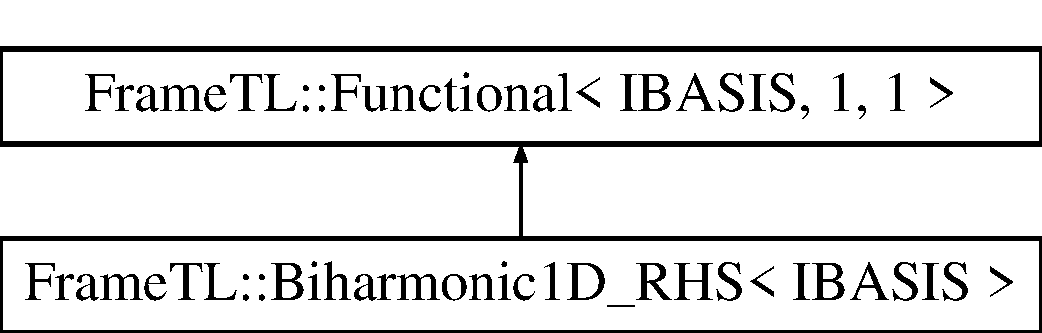
\includegraphics[height=2cm]{classFrameTL_1_1Biharmonic1D__RHS}
\end{center}
\end{figure}
\subsection*{Public Member Functions}
\begin{CompactItemize}
\item 
\hyperlink{classFrameTL_1_1Biharmonic1D__RHS_c9600ba95f7c01ef6080a4372e0d3031}{Biharmonic1D\_\-RHS} (const \hyperlink{classFrameTL_1_1AggregatedFrame}{AggregatedFrame}$<$ IBASIS, 1 $>$ $\ast$frame)
\item 
virtual \hyperlink{classFrameTL_1_1Biharmonic1D__RHS_4b3957bc2e77d88486b21916c7a74030}{$\sim$Biharmonic1D\_\-RHS} ()
\item 
virtual double \hyperlink{classFrameTL_1_1Biharmonic1D__RHS_81cf28300f5a4991eea662f403b5ae88}{evaluate} (const typename \hyperlink{classFrameTL_1_1AggregatedFrame}{AggregatedFrame}$<$ IBASIS, 1 $>$::Index \&lambda) const 
\end{CompactItemize}


\subsection{Detailed Description}
\subsubsection*{template$<$class IBASIS$>$ class FrameTL::Biharmonic1D\_\-RHS$<$ IBASIS $>$}

\hyperlink{classFrameTL_1_1Functional}{Functional} for the righthand side of the 1D test case for the biharmonic equation $ v \mapsto 4v'(1/2) - 384v(1/2) - 16 \int_0^1 (\cos(2\pi x)\pi^4-72) * v(x) dx$. 

\subsection{Constructor \& Destructor Documentation}
\hypertarget{classFrameTL_1_1Biharmonic1D__RHS_c9600ba95f7c01ef6080a4372e0d3031}{
\index{FrameTL::Biharmonic1D\_\-RHS@{FrameTL::Biharmonic1D\_\-RHS}!Biharmonic1D\_\-RHS@{Biharmonic1D\_\-RHS}}
\index{Biharmonic1D\_\-RHS@{Biharmonic1D\_\-RHS}!FrameTL::Biharmonic1D_RHS@{FrameTL::Biharmonic1D\_\-RHS}}
\subsubsection[{Biharmonic1D\_\-RHS}]{\setlength{\rightskip}{0pt plus 5cm}template$<$class IBASIS $>$ {\bf FrameTL::Biharmonic1D\_\-RHS}$<$ IBASIS $>$::{\bf Biharmonic1D\_\-RHS} (const {\bf AggregatedFrame}$<$ IBASIS, 1 $>$ $\ast$ {\em frame})\hspace{0.3cm}{\tt  \mbox{[}inline\mbox{]}}}}
\label{classFrameTL_1_1Biharmonic1D__RHS_c9600ba95f7c01ef6080a4372e0d3031}


Constructor with an instance of a frame. \hypertarget{classFrameTL_1_1Biharmonic1D__RHS_4b3957bc2e77d88486b21916c7a74030}{
\index{FrameTL::Biharmonic1D\_\-RHS@{FrameTL::Biharmonic1D\_\-RHS}!$\sim$Biharmonic1D\_\-RHS@{$\sim$Biharmonic1D\_\-RHS}}
\index{$\sim$Biharmonic1D\_\-RHS@{$\sim$Biharmonic1D\_\-RHS}!FrameTL::Biharmonic1D_RHS@{FrameTL::Biharmonic1D\_\-RHS}}
\subsubsection[{$\sim$Biharmonic1D\_\-RHS}]{\setlength{\rightskip}{0pt plus 5cm}template$<$class IBASIS $>$ virtual {\bf FrameTL::Biharmonic1D\_\-RHS}$<$ IBASIS $>$::$\sim${\bf Biharmonic1D\_\-RHS} ()\hspace{0.3cm}{\tt  \mbox{[}inline, virtual\mbox{]}}}}
\label{classFrameTL_1_1Biharmonic1D__RHS_4b3957bc2e77d88486b21916c7a74030}


Virtual destructor. 

\subsection{Member Function Documentation}
\hypertarget{classFrameTL_1_1Biharmonic1D__RHS_81cf28300f5a4991eea662f403b5ae88}{
\index{FrameTL::Biharmonic1D\_\-RHS@{FrameTL::Biharmonic1D\_\-RHS}!evaluate@{evaluate}}
\index{evaluate@{evaluate}!FrameTL::Biharmonic1D_RHS@{FrameTL::Biharmonic1D\_\-RHS}}
\subsubsection[{evaluate}]{\setlength{\rightskip}{0pt plus 5cm}template$<$class IBASIS $>$ double {\bf FrameTL::Biharmonic1D\_\-RHS}$<$ IBASIS $>$::evaluate (const typename {\bf AggregatedFrame}$<$ IBASIS, 1 $>$::Index \& {\em lambda}) const\hspace{0.3cm}{\tt  \mbox{[}inline, virtual\mbox{]}}}}
\label{classFrameTL_1_1Biharmonic1D__RHS_81cf28300f5a4991eea662f403b5ae88}


Evaluate the functional with the wavelet with given index lambda. 

The documentation for this class was generated from the following files:\begin{CompactItemize}
\item 
/home/werner/PROMOTION/source/FrameTL/biharmonic\_\-1d\_\-testcase.h\item 
/home/werner/PROMOTION/source/FrameTL/biharmonic\_\-1d\_\-testcase.cpp\end{CompactItemize}

\hypertarget{classFrameTL_1_1Biharmonic1D__RHS__Integrand}{
\section{FrameTL::Biharmonic1D\_\-RHS\_\-Integrand Class Reference}
\label{classFrameTL_1_1Biharmonic1D__RHS__Integrand}\index{FrameTL::Biharmonic1D\_\-RHS\_\-Integrand@{FrameTL::Biharmonic1D\_\-RHS\_\-Integrand}}
}
{\tt \#include $<$biharmonic\_\-1d\_\-testcase.h$>$}

Inherits MathTL::Function$<$1$>$.

\subsection*{Public Member Functions}
\begin{CompactItemize}
\item 
\hypertarget{classFrameTL_1_1Biharmonic1D__RHS__Integrand_174357ca2c524475a0d66b98375a7ccb}{
double \hyperlink{classFrameTL_1_1Biharmonic1D__RHS__Integrand_174357ca2c524475a0d66b98375a7ccb}{value} (const Point$<$ 1 $>$ \&p, const unsigned int component=0) const }
\label{classFrameTL_1_1Biharmonic1D__RHS__Integrand_174357ca2c524475a0d66b98375a7ccb}

\begin{CompactList}\small\item\em Point evaluation. \item\end{CompactList}\item 
\hypertarget{classFrameTL_1_1Biharmonic1D__RHS__Integrand_6de019d91743507faf5f828c39e0327b}{
void \hyperlink{classFrameTL_1_1Biharmonic1D__RHS__Integrand_6de019d91743507faf5f828c39e0327b}{vector\_\-value} (const Point$<$ 1 $>$ \&p, Vector$<$ double $>$ \&values) const }
\label{classFrameTL_1_1Biharmonic1D__RHS__Integrand_6de019d91743507faf5f828c39e0327b}

\begin{CompactList}\small\item\em Dummy concretisation for the compiler. \item\end{CompactList}\end{CompactItemize}


\subsection{Detailed Description}
A class inheriting from Function$<$1$>$, modeling the function f of the integrand in $\int v(x) f(x) dx$. 

The documentation for this class was generated from the following files:\begin{CompactItemize}
\item 
/home/werner/PROMOTION/source/FrameTL/biharmonic\_\-1d\_\-testcase.h\item 
/home/werner/PROMOTION/source/FrameTL/biharmonic\_\-1d\_\-testcase.cpp\end{CompactItemize}

\hypertarget{classFrameTL_1_1Biharmonic1D__Solution}{
\section{FrameTL::Biharmonic1D\_\-Solution Class Reference}
\label{classFrameTL_1_1Biharmonic1D__Solution}\index{FrameTL::Biharmonic1D\_\-Solution@{FrameTL::Biharmonic1D\_\-Solution}}
}
{\tt \#include $<$biharmonic\_\-1d\_\-testcase.h$>$}

Inherits MathTL::Function$<$ 1 $>$.

\subsection*{Public Member Functions}
\begin{CompactItemize}
\item 
\hypertarget{classFrameTL_1_1Biharmonic1D__Solution_0ac47ada14854cf3055e551c24c15d23}{
\hyperlink{classFrameTL_1_1Biharmonic1D__Solution_0ac47ada14854cf3055e551c24c15d23}{Biharmonic1D\_\-Solution} ()}
\label{classFrameTL_1_1Biharmonic1D__Solution_0ac47ada14854cf3055e551c24c15d23}

\begin{CompactList}\small\item\em Default constructor. \item\end{CompactList}\item 
\hypertarget{classFrameTL_1_1Biharmonic1D__Solution_24f451d77510c4e288e0bdf7fb7b5034}{
double \hyperlink{classFrameTL_1_1Biharmonic1D__Solution_24f451d77510c4e288e0bdf7fb7b5034}{value} (const Point$<$ 1 $>$ \&p, const unsigned int component=0) const }
\label{classFrameTL_1_1Biharmonic1D__Solution_24f451d77510c4e288e0bdf7fb7b5034}

\begin{CompactList}\small\item\em Point evaluation. \item\end{CompactList}\item 
\hypertarget{classFrameTL_1_1Biharmonic1D__Solution_06eca619ffab0ade6671bcdd9bdd15ae}{
void \hyperlink{classFrameTL_1_1Biharmonic1D__Solution_06eca619ffab0ade6671bcdd9bdd15ae}{vector\_\-value} (const Point$<$ 1 $>$ \&p, Vector$<$ double $>$ \&values) const }
\label{classFrameTL_1_1Biharmonic1D__Solution_06eca619ffab0ade6671bcdd9bdd15ae}

\begin{CompactList}\small\item\em Dummy concretisation for the compiler. \item\end{CompactList}\end{CompactItemize}


\subsection{Detailed Description}
Exact solution for the test case for the one-dimensional biharmonic equation, $u(x) = -\cos(2\pi x)+1 + p(x)$ with $p(x) = 48x^4-63x^3+47/2x^2$, for $0 \leq x < 1/2$, $p(x) = 48x^4-127x^3+235/2x^2-46x+15/2$, for $1/2 \leq x \leq 1$ 

The documentation for this class was generated from the following files:\begin{CompactItemize}
\item 
/home/werner/PROMOTION/source/FrameTL/biharmonic\_\-1d\_\-testcase.h\item 
/home/werner/PROMOTION/source/FrameTL/biharmonic\_\-1d\_\-testcase.cpp\end{CompactItemize}

\hypertarget{classFrameTL_1_1BiharmonicEquation}{
\section{FrameTL::BiharmonicEquation$<$ IBASIS, DIM $>$ Class Template Reference}
\label{classFrameTL_1_1BiharmonicEquation}\index{FrameTL::BiharmonicEquation@{FrameTL::BiharmonicEquation}}
}
{\tt \#include $<$biharmonic\_\-equation.h$>$}

Inherits WaveletTL::FullyDiagonalEnergyNormPreconditioner$<$AggregatedFrame$<$IBASIS,DIM$>$::Index$>$.

\subsection*{Public Types}
\begin{CompactItemize}
\item 
\hyperlink{structtypedef}{typedef} \hyperlink{classFrameTL_1_1AggregatedFrame}{AggregatedFrame}$<$ IBASIS, DIM $>$ \hyperlink{classFrameTL_1_1BiharmonicEquation_a6589dcf7cfc46ba411c3f35146e1a5d}{Frame}
\item 
\hyperlink{structtypedef}{typedef} \hyperlink{classFrameTL_1_1AggregatedFrame}{AggregatedFrame}$<$ IBASIS, DIM $>$ \hyperlink{classFrameTL_1_1BiharmonicEquation_2c96ea759f7da9b09717e9a68eb49a6f}{WaveletBasis}
\item 
\hyperlink{structtypedef}{typedef} \hyperlink{classFrameTL_1_1FrameIndex}{Frame::Index} \hyperlink{classFrameTL_1_1BiharmonicEquation_3092eb11291bea911cf17d1de560bc1e}{Index}
\end{CompactItemize}
\subsection*{Public Member Functions}
\begin{CompactItemize}
\item 
\hyperlink{classFrameTL_1_1BiharmonicEquation_92657a3e07a5df0a73cb50563212a081}{BiharmonicEquation} (const BiharmonicBVP$<$ DIM $>$ $\ast$bih\_\-bvp, const \hyperlink{classFrameTL_1_1AggregatedFrame}{AggregatedFrame}$<$ IBASIS, DIM $>$ $\ast$frame, const int jmax)
\item 
const \hyperlink{classFrameTL_1_1AggregatedFrame}{AggregatedFrame}$<$ IBASIS, DIM $>$ \& \hyperlink{classFrameTL_1_1BiharmonicEquation_4c9be93d423d6e61f61fa31b998d559d}{frame} () const 
\item 
const BiharmonicBVP$<$ DIM $>$ \& \hyperlink{classFrameTL_1_1BiharmonicEquation_b688202abfc6f7d72a04dbf365ba6809}{get\_\-bvp} () const 
\item 
const \hyperlink{classFrameTL_1_1AggregatedFrame}{AggregatedFrame}$<$ IBASIS, DIM $>$ \& \hyperlink{classFrameTL_1_1BiharmonicEquation_f197bfb03a8f123739a3311d803a1803}{basis} () const 
\item 
double \hyperlink{classFrameTL_1_1BiharmonicEquation_d16c3e0cfbdc25d321fece0ce1e7069e}{D} (const typename \hyperlink{classFrameTL_1_1AggregatedFrame}{AggregatedFrame}$<$ IBASIS, DIM $>$::\hyperlink{classFrameTL_1_1FrameIndex}{Index} \&lambda) const 
\item 
double \hyperlink{classFrameTL_1_1BiharmonicEquation_7e489f4287862dad10b3334316bf786a}{a} (const typename \hyperlink{classFrameTL_1_1AggregatedFrame}{AggregatedFrame}$<$ IBASIS, DIM $>$::\hyperlink{classFrameTL_1_1FrameIndex}{Index} \&lambda, const typename \hyperlink{classFrameTL_1_1AggregatedFrame}{AggregatedFrame}$<$ IBASIS, DIM $>$::\hyperlink{classFrameTL_1_1FrameIndex}{Index} \&nu) const 
\item 
double \hyperlink{classFrameTL_1_1BiharmonicEquation_14e15fda0b1f3cc901cb3a3026ceb536}{norm\_\-A} () const 
\item 
void \hyperlink{classFrameTL_1_1BiharmonicEquation_731c3491306a23684256fe4dede66b53}{set\_\-norm\_\-A} (const double \_\-normA)
\item 
void \hyperlink{classFrameTL_1_1BiharmonicEquation_390c7b64b0183610aede9842c805804e}{set\_\-Ainv} (const double nAinv)
\item 
double \hyperlink{classFrameTL_1_1BiharmonicEquation_c619e416f851afd5a307014a69cc6d35}{s\_\-star} () const 
\item 
double \hyperlink{classFrameTL_1_1BiharmonicEquation_9f424ae1bc3dbcc5490e6bd77240c71c}{alphak} (const unsigned int k) const 
\item 
double \hyperlink{classFrameTL_1_1BiharmonicEquation_0b477b96020f82cbccb11d904acbaf3e}{f} (const typename \hyperlink{classFrameTL_1_1AggregatedFrame}{AggregatedFrame}$<$ IBASIS, DIM $>$::\hyperlink{classFrameTL_1_1FrameIndex}{Index} \&lambda) const 
\item 
void \hyperlink{classFrameTL_1_1BiharmonicEquation_032b924e5b4f43048535d3f2544eb27d}{RHS} (const double eta, InfiniteVector$<$ double, typename \hyperlink{classFrameTL_1_1AggregatedFrame}{AggregatedFrame}$<$ IBASIS, DIM $>$::\hyperlink{classFrameTL_1_1FrameIndex}{Index} $>$ \&coeffs) const 
\item 
double \hyperlink{classFrameTL_1_1BiharmonicEquation_8a83415dd882a4f51ceeaa46c988462f}{F\_\-norm} () const 
\item 
void \hyperlink{classFrameTL_1_1BiharmonicEquation_cf2416d4c035dbe3edf426d8ca032c0f}{set\_\-bvp} (const BiharmonicBVP$<$ DIM $>$ $\ast$)
\end{CompactItemize}
\subsection*{Static Public Member Functions}
\begin{CompactItemize}
\item 
static bool \hyperlink{classFrameTL_1_1BiharmonicEquation_9d20dc4a94ba5719b1a25c92e8faba10}{local\_\-operator} ()
\item 
static double \hyperlink{classFrameTL_1_1BiharmonicEquation_89f12c9466f7e91a5dc94c45525ee17f}{operator\_\-order} ()
\end{CompactItemize}
\subsection*{Static Public Attributes}
\begin{CompactItemize}
\item 
static const int \hyperlink{classFrameTL_1_1BiharmonicEquation_8c79fee355dd2f68f56cd70a94e55511}{space\_\-dimension} = DIM
\end{CompactItemize}
\subsection*{Protected Types}
\begin{CompactItemize}
\item 
\hypertarget{classFrameTL_1_1BiharmonicEquation_357fd07037f8d50a367adbeec07a8e99}{
\hyperlink{structtypedef}{typedef} std::map$<$ \hyperlink{classFrameTL_1_1Index1D}{Index1D}$<$ IBASIS $>$, double $>$ \textbf{Column1D}}
\label{classFrameTL_1_1BiharmonicEquation_357fd07037f8d50a367adbeec07a8e99}

\item 
\hypertarget{classFrameTL_1_1BiharmonicEquation_5f4aca4d0f0e006e73fa4c1dfa9641bb}{
\hyperlink{structtypedef}{typedef} std::map$<$ \hyperlink{classFrameTL_1_1Index1D}{Index1D}$<$ IBASIS $>$, Column1D $>$ \textbf{One\_\-D\_\-IntegralCache}}
\label{classFrameTL_1_1BiharmonicEquation_5f4aca4d0f0e006e73fa4c1dfa9641bb}

\end{CompactItemize}
\subsection*{Protected Attributes}
\begin{CompactItemize}
\item 
const BiharmonicBVP$<$ DIM $>$ $\ast$ \hyperlink{classFrameTL_1_1BiharmonicEquation_31755efe61c40e44592198e134e4e2d0}{bih\_\-bvp\_\-}
\item 
\hypertarget{classFrameTL_1_1BiharmonicEquation_66b6d2b9b300fd8c2dab7f633cb938aa}{
const \hyperlink{classFrameTL_1_1AggregatedFrame}{AggregatedFrame}$<$ IBASIS, DIM $>$ $\ast$ \textbf{frame\_\-}}
\label{classFrameTL_1_1BiharmonicEquation_66b6d2b9b300fd8c2dab7f633cb938aa}

\item 
\hypertarget{classFrameTL_1_1BiharmonicEquation_70038960d2611b86152148d29c7e416d}{
const int \textbf{jmax\_\-}}
\label{classFrameTL_1_1BiharmonicEquation_70038960d2611b86152148d29c7e416d}

\item 
One\_\-D\_\-IntegralCache \hyperlink{classFrameTL_1_1BiharmonicEquation_86bca5b3462307b9a3f20cd6f84c0e0f}{one\_\-d\_\-integrals}
\end{CompactItemize}


\subsection{Detailed Description}
\subsubsection*{template$<$class IBASIS, unsigned int DIM$>$ class FrameTL::BiharmonicEquation$<$ IBASIS, DIM $>$}

This class models the (preconditioned) infinite-dimensional matrix problem

Au = D$^\wedge$\{-1\}LD$^\wedge$\{-1\}u = D$^\wedge$\{-1\}F

when reformulating a symmetric, forth-order elliptic boundary value problem in divergence form over some domain Omega in R$^\wedge$d with boundary Gamma=dOmega, with homogeneous Dirichlet/Neumann/Robin boundary conditions

-Delta$^\wedge$2 u(x) = f(x) in Omega u(x) = 0 on Gamma\_\-D du/dn(x) = 0 on Gamma.

The corresponding bilinear form in

L = (a(,))\_\-\{,\}

is

a(u,v) =  $<$Delta u(x), Delta v(x)$>$ dx

and the right-hand side is

f(v) =  f(x)$\ast$v(x) dx.

The evaluation of a(.,.) and f is possible for arguments  which stem from an aggregated wavelet frame =$\backslash$\} of the corresponding function space over Omega. 

\subsection{Member Typedef Documentation}
\hypertarget{classFrameTL_1_1BiharmonicEquation_a6589dcf7cfc46ba411c3f35146e1a5d}{
\index{FrameTL::BiharmonicEquation@{FrameTL::BiharmonicEquation}!Frame@{Frame}}
\index{Frame@{Frame}!FrameTL::BiharmonicEquation@{FrameTL::BiharmonicEquation}}
\subsubsection[{Frame}]{\setlength{\rightskip}{0pt plus 5cm}template$<$class IBASIS , unsigned int DIM$>$ {\bf typedef} {\bf AggregatedFrame}$<$IBASIS,DIM$>$ {\bf FrameTL::BiharmonicEquation}$<$ IBASIS, DIM $>$::{\bf Frame}}}
\label{classFrameTL_1_1BiharmonicEquation_a6589dcf7cfc46ba411c3f35146e1a5d}


make template argument accessible \hypertarget{classFrameTL_1_1BiharmonicEquation_3092eb11291bea911cf17d1de560bc1e}{
\index{FrameTL::BiharmonicEquation@{FrameTL::BiharmonicEquation}!Index@{Index}}
\index{Index@{Index}!FrameTL::BiharmonicEquation@{FrameTL::BiharmonicEquation}}
\subsubsection[{Index}]{\setlength{\rightskip}{0pt plus 5cm}template$<$class IBASIS , unsigned int DIM$>$ {\bf typedef} {\bf Frame::Index} {\bf FrameTL::BiharmonicEquation}$<$ IBASIS, DIM $>$::{\bf Index}}}
\label{classFrameTL_1_1BiharmonicEquation_3092eb11291bea911cf17d1de560bc1e}


make template argument accessible \hypertarget{classFrameTL_1_1BiharmonicEquation_2c96ea759f7da9b09717e9a68eb49a6f}{
\index{FrameTL::BiharmonicEquation@{FrameTL::BiharmonicEquation}!WaveletBasis@{WaveletBasis}}
\index{WaveletBasis@{WaveletBasis}!FrameTL::BiharmonicEquation@{FrameTL::BiharmonicEquation}}
\subsubsection[{WaveletBasis}]{\setlength{\rightskip}{0pt plus 5cm}template$<$class IBASIS , unsigned int DIM$>$ {\bf typedef} {\bf AggregatedFrame}$<$IBASIS,DIM$>$ {\bf FrameTL::BiharmonicEquation}$<$ IBASIS, DIM $>$::{\bf WaveletBasis}}}
\label{classFrameTL_1_1BiharmonicEquation_2c96ea759f7da9b09717e9a68eb49a6f}


dummy \hyperlink{structtypedef}{typedef} to be compatible with WaveletTL routines 

\subsection{Constructor \& Destructor Documentation}
\hypertarget{classFrameTL_1_1BiharmonicEquation_92657a3e07a5df0a73cb50563212a081}{
\index{FrameTL::BiharmonicEquation@{FrameTL::BiharmonicEquation}!BiharmonicEquation@{BiharmonicEquation}}
\index{BiharmonicEquation@{BiharmonicEquation}!FrameTL::BiharmonicEquation@{FrameTL::BiharmonicEquation}}
\subsubsection[{BiharmonicEquation}]{\setlength{\rightskip}{0pt plus 5cm}template$<$class IBASIS , unsigned int DIM$>$ {\bf FrameTL::BiharmonicEquation}$<$ IBASIS, DIM $>$::{\bf BiharmonicEquation} (const BiharmonicBVP$<$ DIM $>$ $\ast$ {\em bih\_\-bvp}, \/  const {\bf AggregatedFrame}$<$ IBASIS, DIM $>$ $\ast$ {\em frame}, \/  const int {\em jmax})\hspace{0.3cm}{\tt  \mbox{[}inline\mbox{]}}}}
\label{classFrameTL_1_1BiharmonicEquation_92657a3e07a5df0a73cb50563212a081}


constructor 

\subsection{Member Function Documentation}
\hypertarget{classFrameTL_1_1BiharmonicEquation_7e489f4287862dad10b3334316bf786a}{
\index{FrameTL::BiharmonicEquation@{FrameTL::BiharmonicEquation}!a@{a}}
\index{a@{a}!FrameTL::BiharmonicEquation@{FrameTL::BiharmonicEquation}}
\subsubsection[{a}]{\setlength{\rightskip}{0pt plus 5cm}template$<$class IBASIS , unsigned int DIM$>$ double {\bf FrameTL::BiharmonicEquation}$<$ IBASIS, DIM $>$::a (const typename {\bf AggregatedFrame}$<$ IBASIS, DIM $>$::{\bf Index} \& {\em lambda}, \/  const typename {\bf AggregatedFrame}$<$ IBASIS, DIM $>$::{\bf Index} \& {\em nu}) const\hspace{0.3cm}{\tt  \mbox{[}inline\mbox{]}}}}
\label{classFrameTL_1_1BiharmonicEquation_7e489f4287862dad10b3334316bf786a}


evaluate the (unpreconditioned) bilinear form a; \hypertarget{classFrameTL_1_1BiharmonicEquation_9f424ae1bc3dbcc5490e6bd77240c71c}{
\index{FrameTL::BiharmonicEquation@{FrameTL::BiharmonicEquation}!alphak@{alphak}}
\index{alphak@{alphak}!FrameTL::BiharmonicEquation@{FrameTL::BiharmonicEquation}}
\subsubsection[{alphak}]{\setlength{\rightskip}{0pt plus 5cm}template$<$class IBASIS , unsigned int DIM$>$ double {\bf FrameTL::BiharmonicEquation}$<$ IBASIS, DIM $>$::alphak (const unsigned int {\em k}) const\hspace{0.3cm}{\tt  \mbox{[}inline\mbox{]}}}}
\label{classFrameTL_1_1BiharmonicEquation_9f424ae1bc3dbcc5490e6bd77240c71c}


estimate the compression constants alpha\_\-k in $|$$|$A-A\_\-k$|$$|$ $<$= alpha\_\-k $\ast$ 2$^\wedge$\{-s$\ast$k\} \hypertarget{classFrameTL_1_1BiharmonicEquation_f197bfb03a8f123739a3311d803a1803}{
\index{FrameTL::BiharmonicEquation@{FrameTL::BiharmonicEquation}!basis@{basis}}
\index{basis@{basis}!FrameTL::BiharmonicEquation@{FrameTL::BiharmonicEquation}}
\subsubsection[{basis}]{\setlength{\rightskip}{0pt plus 5cm}template$<$class IBASIS , unsigned int DIM$>$ const {\bf AggregatedFrame}$<$IBASIS,DIM$>$\& {\bf FrameTL::BiharmonicEquation}$<$ IBASIS, DIM $>$::basis () const\hspace{0.3cm}{\tt  \mbox{[}inline\mbox{]}}}}
\label{classFrameTL_1_1BiharmonicEquation_f197bfb03a8f123739a3311d803a1803}


read access to the frame but with a somewhat weird function name. this is just a first hack to be able to use routines in WaveletTL's compression.h \hypertarget{classFrameTL_1_1BiharmonicEquation_d16c3e0cfbdc25d321fece0ce1e7069e}{
\index{FrameTL::BiharmonicEquation@{FrameTL::BiharmonicEquation}!D@{D}}
\index{D@{D}!FrameTL::BiharmonicEquation@{FrameTL::BiharmonicEquation}}
\subsubsection[{D}]{\setlength{\rightskip}{0pt plus 5cm}template$<$class IBASIS , unsigned int DIM$>$ double {\bf FrameTL::BiharmonicEquation}$<$ IBASIS, DIM $>$::D (const typename {\bf AggregatedFrame}$<$ IBASIS, DIM $>$::{\bf Index} \& {\em lambda}) const\hspace{0.3cm}{\tt  \mbox{[}inline\mbox{]}}}}
\label{classFrameTL_1_1BiharmonicEquation_d16c3e0cfbdc25d321fece0ce1e7069e}


evaluate the diagonal preconditioner D \hypertarget{classFrameTL_1_1BiharmonicEquation_0b477b96020f82cbccb11d904acbaf3e}{
\index{FrameTL::BiharmonicEquation@{FrameTL::BiharmonicEquation}!f@{f}}
\index{f@{f}!FrameTL::BiharmonicEquation@{FrameTL::BiharmonicEquation}}
\subsubsection[{f}]{\setlength{\rightskip}{0pt plus 5cm}template$<$class IBASIS , unsigned int DIM$>$ double {\bf FrameTL::BiharmonicEquation}$<$ IBASIS, DIM $>$::f (const typename {\bf AggregatedFrame}$<$ IBASIS, DIM $>$::{\bf Index} \& {\em lambda}) const\hspace{0.3cm}{\tt  \mbox{[}inline\mbox{]}}}}
\label{classFrameTL_1_1BiharmonicEquation_0b477b96020f82cbccb11d904acbaf3e}


evaluate the (unpreconditioned) right-hand side f \hypertarget{classFrameTL_1_1BiharmonicEquation_8a83415dd882a4f51ceeaa46c988462f}{
\index{FrameTL::BiharmonicEquation@{FrameTL::BiharmonicEquation}!F\_\-norm@{F\_\-norm}}
\index{F\_\-norm@{F\_\-norm}!FrameTL::BiharmonicEquation@{FrameTL::BiharmonicEquation}}
\subsubsection[{F\_\-norm}]{\setlength{\rightskip}{0pt plus 5cm}template$<$class IBASIS , unsigned int DIM$>$ double {\bf FrameTL::BiharmonicEquation}$<$ IBASIS, DIM $>$::F\_\-norm () const\hspace{0.3cm}{\tt  \mbox{[}inline\mbox{]}}}}
\label{classFrameTL_1_1BiharmonicEquation_8a83415dd882a4f51ceeaa46c988462f}


compute (or estimate) $|$$|$F$|$$|$\_\-2 \hypertarget{classFrameTL_1_1BiharmonicEquation_4c9be93d423d6e61f61fa31b998d559d}{
\index{FrameTL::BiharmonicEquation@{FrameTL::BiharmonicEquation}!frame@{frame}}
\index{frame@{frame}!FrameTL::BiharmonicEquation@{FrameTL::BiharmonicEquation}}
\subsubsection[{frame}]{\setlength{\rightskip}{0pt plus 5cm}template$<$class IBASIS , unsigned int DIM$>$ const {\bf AggregatedFrame}$<$IBASIS,DIM$>$\& {\bf FrameTL::BiharmonicEquation}$<$ IBASIS, DIM $>$::frame () const\hspace{0.3cm}{\tt  \mbox{[}inline\mbox{]}}}}
\label{classFrameTL_1_1BiharmonicEquation_4c9be93d423d6e61f61fa31b998d559d}


read access to the frame \hypertarget{classFrameTL_1_1BiharmonicEquation_b688202abfc6f7d72a04dbf365ba6809}{
\index{FrameTL::BiharmonicEquation@{FrameTL::BiharmonicEquation}!get\_\-bvp@{get\_\-bvp}}
\index{get\_\-bvp@{get\_\-bvp}!FrameTL::BiharmonicEquation@{FrameTL::BiharmonicEquation}}
\subsubsection[{get\_\-bvp}]{\setlength{\rightskip}{0pt plus 5cm}template$<$class IBASIS , unsigned int DIM$>$ const BiharmonicBVP$<$DIM$>$\& {\bf FrameTL::BiharmonicEquation}$<$ IBASIS, DIM $>$::get\_\-bvp () const\hspace{0.3cm}{\tt  \mbox{[}inline\mbox{]}}}}
\label{classFrameTL_1_1BiharmonicEquation_b688202abfc6f7d72a04dbf365ba6809}


get the boundary value problem \hypertarget{classFrameTL_1_1BiharmonicEquation_9d20dc4a94ba5719b1a25c92e8faba10}{
\index{FrameTL::BiharmonicEquation@{FrameTL::BiharmonicEquation}!local\_\-operator@{local\_\-operator}}
\index{local\_\-operator@{local\_\-operator}!FrameTL::BiharmonicEquation@{FrameTL::BiharmonicEquation}}
\subsubsection[{local\_\-operator}]{\setlength{\rightskip}{0pt plus 5cm}template$<$class IBASIS , unsigned int DIM$>$ static bool {\bf FrameTL::BiharmonicEquation}$<$ IBASIS, DIM $>$::local\_\-operator ()\hspace{0.3cm}{\tt  \mbox{[}inline, static\mbox{]}}}}
\label{classFrameTL_1_1BiharmonicEquation_9d20dc4a94ba5719b1a25c92e8faba10}


differential operators are local \hypertarget{classFrameTL_1_1BiharmonicEquation_14e15fda0b1f3cc901cb3a3026ceb536}{
\index{FrameTL::BiharmonicEquation@{FrameTL::BiharmonicEquation}!norm\_\-A@{norm\_\-A}}
\index{norm\_\-A@{norm\_\-A}!FrameTL::BiharmonicEquation@{FrameTL::BiharmonicEquation}}
\subsubsection[{norm\_\-A}]{\setlength{\rightskip}{0pt plus 5cm}template$<$class IBASIS , unsigned int DIM$>$ double {\bf FrameTL::BiharmonicEquation}$<$ IBASIS, DIM $>$::norm\_\-A () const\hspace{0.3cm}{\tt  \mbox{[}inline\mbox{]}}}}
\label{classFrameTL_1_1BiharmonicEquation_14e15fda0b1f3cc901cb3a3026ceb536}


estimate the spectral norm $|$$|$A$|$$|$ \hypertarget{classFrameTL_1_1BiharmonicEquation_89f12c9466f7e91a5dc94c45525ee17f}{
\index{FrameTL::BiharmonicEquation@{FrameTL::BiharmonicEquation}!operator\_\-order@{operator\_\-order}}
\index{operator\_\-order@{operator\_\-order}!FrameTL::BiharmonicEquation@{FrameTL::BiharmonicEquation}}
\subsubsection[{operator\_\-order}]{\setlength{\rightskip}{0pt plus 5cm}template$<$class IBASIS , unsigned int DIM$>$ static double {\bf FrameTL::BiharmonicEquation}$<$ IBASIS, DIM $>$::operator\_\-order ()\hspace{0.3cm}{\tt  \mbox{[}inline, static\mbox{]}}}}
\label{classFrameTL_1_1BiharmonicEquation_89f12c9466f7e91a5dc94c45525ee17f}


order of the operator \hypertarget{classFrameTL_1_1BiharmonicEquation_032b924e5b4f43048535d3f2544eb27d}{
\index{FrameTL::BiharmonicEquation@{FrameTL::BiharmonicEquation}!RHS@{RHS}}
\index{RHS@{RHS}!FrameTL::BiharmonicEquation@{FrameTL::BiharmonicEquation}}
\subsubsection[{RHS}]{\setlength{\rightskip}{0pt plus 5cm}template$<$class IBASIS , unsigned int DIM$>$ void {\bf FrameTL::BiharmonicEquation}$<$ IBASIS, DIM $>$::RHS (const double {\em eta}, \/  InfiniteVector$<$ double, typename {\bf AggregatedFrame}$<$ IBASIS, DIM $>$::{\bf Index} $>$ \& {\em coeffs}) const\hspace{0.3cm}{\tt  \mbox{[}inline\mbox{]}}}}
\label{classFrameTL_1_1BiharmonicEquation_032b924e5b4f43048535d3f2544eb27d}


approximate the wavelet coefficient set of the preconditioned right-hand side F within a prescribed  error tolerance \hypertarget{classFrameTL_1_1BiharmonicEquation_c619e416f851afd5a307014a69cc6d35}{
\index{FrameTL::BiharmonicEquation@{FrameTL::BiharmonicEquation}!s\_\-star@{s\_\-star}}
\index{s\_\-star@{s\_\-star}!FrameTL::BiharmonicEquation@{FrameTL::BiharmonicEquation}}
\subsubsection[{s\_\-star}]{\setlength{\rightskip}{0pt plus 5cm}template$<$class IBASIS , unsigned int DIM$>$ double {\bf FrameTL::BiharmonicEquation}$<$ IBASIS, DIM $>$::s\_\-star () const\hspace{0.3cm}{\tt  \mbox{[}inline\mbox{]}}}}
\label{classFrameTL_1_1BiharmonicEquation_c619e416f851afd5a307014a69cc6d35}


estimate compressibility exponent s$^\wedge$$\ast$ \hypertarget{classFrameTL_1_1BiharmonicEquation_390c7b64b0183610aede9842c805804e}{
\index{FrameTL::BiharmonicEquation@{FrameTL::BiharmonicEquation}!set\_\-Ainv@{set\_\-Ainv}}
\index{set\_\-Ainv@{set\_\-Ainv}!FrameTL::BiharmonicEquation@{FrameTL::BiharmonicEquation}}
\subsubsection[{set\_\-Ainv}]{\setlength{\rightskip}{0pt plus 5cm}template$<$class IBASIS , unsigned int DIM$>$ void {\bf FrameTL::BiharmonicEquation}$<$ IBASIS, DIM $>$::set\_\-Ainv (const double {\em nAinv})\hspace{0.3cm}{\tt  \mbox{[}inline\mbox{]}}}}
\label{classFrameTL_1_1BiharmonicEquation_390c7b64b0183610aede9842c805804e}


sets estimate for $|$$|$A$^\wedge$\{-1\}$|$$|$ \hypertarget{classFrameTL_1_1BiharmonicEquation_cf2416d4c035dbe3edf426d8ca032c0f}{
\index{FrameTL::BiharmonicEquation@{FrameTL::BiharmonicEquation}!set\_\-bvp@{set\_\-bvp}}
\index{set\_\-bvp@{set\_\-bvp}!FrameTL::BiharmonicEquation@{FrameTL::BiharmonicEquation}}
\subsubsection[{set\_\-bvp}]{\setlength{\rightskip}{0pt plus 5cm}template$<$class IBASIS , unsigned int DIM$>$ void {\bf FrameTL::BiharmonicEquation}$<$ IBASIS, DIM $>$::set\_\-bvp (const BiharmonicBVP$<$ DIM $>$ $\ast$)}}
\label{classFrameTL_1_1BiharmonicEquation_cf2416d4c035dbe3edf426d8ca032c0f}


set the boundary value problem \hypertarget{classFrameTL_1_1BiharmonicEquation_731c3491306a23684256fe4dede66b53}{
\index{FrameTL::BiharmonicEquation@{FrameTL::BiharmonicEquation}!set\_\-norm\_\-A@{set\_\-norm\_\-A}}
\index{set\_\-norm\_\-A@{set\_\-norm\_\-A}!FrameTL::BiharmonicEquation@{FrameTL::BiharmonicEquation}}
\subsubsection[{set\_\-norm\_\-A}]{\setlength{\rightskip}{0pt plus 5cm}template$<$class IBASIS , unsigned int DIM$>$ void {\bf FrameTL::BiharmonicEquation}$<$ IBASIS, DIM $>$::set\_\-norm\_\-A (const double {\em \_\-normA})\hspace{0.3cm}{\tt  \mbox{[}inline\mbox{]}}}}
\label{classFrameTL_1_1BiharmonicEquation_731c3491306a23684256fe4dede66b53}


sets estimate for $|$$|$A$|$$|$ 

\subsection{Member Data Documentation}
\hypertarget{classFrameTL_1_1BiharmonicEquation_31755efe61c40e44592198e134e4e2d0}{
\index{FrameTL::BiharmonicEquation@{FrameTL::BiharmonicEquation}!bih\_\-bvp\_\-@{bih\_\-bvp\_\-}}
\index{bih\_\-bvp\_\-@{bih\_\-bvp\_\-}!FrameTL::BiharmonicEquation@{FrameTL::BiharmonicEquation}}
\subsubsection[{bih\_\-bvp\_\-}]{\setlength{\rightskip}{0pt plus 5cm}template$<$class IBASIS , unsigned int DIM$>$ const BiharmonicBVP$<$DIM$>$$\ast$ {\bf FrameTL::BiharmonicEquation}$<$ IBASIS, DIM $>$::{\bf bih\_\-bvp\_\-}\hspace{0.3cm}{\tt  \mbox{[}protected\mbox{]}}}}
\label{classFrameTL_1_1BiharmonicEquation_31755efe61c40e44592198e134e4e2d0}


corresponding elliptic boundary value problem \hypertarget{classFrameTL_1_1BiharmonicEquation_86bca5b3462307b9a3f20cd6f84c0e0f}{
\index{FrameTL::BiharmonicEquation@{FrameTL::BiharmonicEquation}!one\_\-d\_\-integrals@{one\_\-d\_\-integrals}}
\index{one\_\-d\_\-integrals@{one\_\-d\_\-integrals}!FrameTL::BiharmonicEquation@{FrameTL::BiharmonicEquation}}
\subsubsection[{one\_\-d\_\-integrals}]{\setlength{\rightskip}{0pt plus 5cm}template$<$class IBASIS , unsigned int DIM$>$ One\_\-D\_\-IntegralCache {\bf FrameTL::BiharmonicEquation}$<$ IBASIS, DIM $>$::{\bf one\_\-d\_\-integrals}\hspace{0.3cm}{\tt  \mbox{[}mutable, protected\mbox{]}}}}
\label{classFrameTL_1_1BiharmonicEquation_86bca5b3462307b9a3f20cd6f84c0e0f}


cache for one dimensional integrals ONLY USED TOGETHER WITH TrivialAffine QUADRATURE RULE OPTION \hypertarget{classFrameTL_1_1BiharmonicEquation_8c79fee355dd2f68f56cd70a94e55511}{
\index{FrameTL::BiharmonicEquation@{FrameTL::BiharmonicEquation}!space\_\-dimension@{space\_\-dimension}}
\index{space\_\-dimension@{space\_\-dimension}!FrameTL::BiharmonicEquation@{FrameTL::BiharmonicEquation}}
\subsubsection[{space\_\-dimension}]{\setlength{\rightskip}{0pt plus 5cm}template$<$class IBASIS , unsigned int DIM$>$ const int {\bf FrameTL::BiharmonicEquation}$<$ IBASIS, DIM $>$::{\bf space\_\-dimension} = DIM\hspace{0.3cm}{\tt  \mbox{[}static\mbox{]}}}}
\label{classFrameTL_1_1BiharmonicEquation_8c79fee355dd2f68f56cd70a94e55511}


space dimension of the problem 

The documentation for this class was generated from the following files:\begin{CompactItemize}
\item 
/home/werner/PROMOTION/source/FrameTL/biharmonic\_\-equation.h\item 
/home/werner/PROMOTION/source/FrameTL/biharmonic\_\-equation.cpp\end{CompactItemize}

\hypertarget{structFrameTL_1_1Coefficient}{
\section{FrameTL::Coefficient Struct Reference}
\label{structFrameTL_1_1Coefficient}\index{FrameTL::Coefficient@{FrameTL::Coefficient}}
}
{\tt \#include $<$frame\_\-index.h$>$}

\subsection*{Public Attributes}
\begin{CompactItemize}
\item 
\hypertarget{structFrameTL_1_1Coefficient_cffca2b027806c7b010ece103a1e63b2}{
int \hyperlink{structFrameTL_1_1Coefficient_cffca2b027806c7b010ece103a1e63b2}{num}}
\label{structFrameTL_1_1Coefficient_cffca2b027806c7b010ece103a1e63b2}

\begin{CompactList}\small\item\em Will be used to represent the number of a frame index. \item\end{CompactList}\item 
\hypertarget{structFrameTL_1_1Coefficient_a0e2160c3b1f0593a875a109bca1444a}{
double \hyperlink{structFrameTL_1_1Coefficient_a0e2160c3b1f0593a875a109bca1444a}{val}}
\label{structFrameTL_1_1Coefficient_a0e2160c3b1f0593a875a109bca1444a}

\begin{CompactList}\small\item\em One coefficient of a frame expansion corresponding to the frame index given by 'num'. \item\end{CompactList}\end{CompactItemize}


\subsection{Detailed Description}
A simple type representing pairs of a frame index, given by its number, and a double valued coefficient in a frame expansion. It shall be used as replacement for a pair of frame\_\-index and coeffient value. 

The documentation for this struct was generated from the following file:\begin{CompactItemize}
\item 
/home/werner/PROMOTION/source/FrameTL/frame\_\-index.h\end{CompactItemize}

\hypertarget{classFrameTL_1_1EllipticEquation}{
\section{FrameTL::EllipticEquation$<$ IBASIS, DIM $>$ Class Template Reference}
\label{classFrameTL_1_1EllipticEquation}\index{FrameTL::EllipticEquation@{FrameTL::EllipticEquation}}
}
{\tt \#include $<$elliptic\_\-equation.h$>$}

Inherits WaveletTL::FullyDiagonalEnergyNormPreconditioner$<$AggregatedFrame$<$IBASIS,DIM$>$::Index$>$.

\subsection*{Public Types}
\begin{CompactItemize}
\item 
\hyperlink{structtypedef}{typedef} \hyperlink{classFrameTL_1_1AggregatedFrame}{AggregatedFrame}$<$ IBASIS, DIM $>$ \hyperlink{classFrameTL_1_1EllipticEquation_65fa5216492c8a03f841cf910182a00c}{Frame}
\item 
\hyperlink{structtypedef}{typedef} \hyperlink{classFrameTL_1_1AggregatedFrame}{AggregatedFrame}$<$ IBASIS, DIM $>$ \hyperlink{classFrameTL_1_1EllipticEquation_44b9abebf9c101271d3ddec1ce3ffd3a}{WaveletBasis}
\item 
\hyperlink{structtypedef}{typedef} \hyperlink{classFrameTL_1_1FrameIndex}{Frame::Index} \hyperlink{classFrameTL_1_1EllipticEquation_598c5b4d850e49947abc0a253298e94c}{Index}
\end{CompactItemize}
\subsection*{Public Member Functions}
\begin{CompactItemize}
\item 
\hyperlink{classFrameTL_1_1EllipticEquation_44b302a82e544d16d49cf6b4dab933b0}{EllipticEquation} (const EllipticBVP$<$ DIM $>$ $\ast$ell\_\-bvp, const \hyperlink{classFrameTL_1_1AggregatedFrame}{AggregatedFrame}$<$ IBASIS, DIM $>$ $\ast$frame, const int jmax)
\item 
const \hyperlink{classFrameTL_1_1AggregatedFrame}{AggregatedFrame}$<$ IBASIS, DIM $>$ \& \hyperlink{classFrameTL_1_1EllipticEquation_49f035460f9c0a08ed1a292bf6d3e7f9}{frame} () const 
\item 
const EllipticBVP$<$ DIM $>$ \& \hyperlink{classFrameTL_1_1EllipticEquation_7574a07220674516f1be1fd38b3fb4cc}{get\_\-bvp} () const 
\item 
const \hyperlink{classFrameTL_1_1AggregatedFrame}{AggregatedFrame}$<$ IBASIS, DIM $>$ \& \hyperlink{classFrameTL_1_1EllipticEquation_f3c3552134fe3d41c4d4d00b13130381}{basis} () const 
\item 
double \hyperlink{classFrameTL_1_1EllipticEquation_a5b30bbacf5d024873268eb979e65748}{operator\_\-order} () const 
\item 
double \hyperlink{classFrameTL_1_1EllipticEquation_f7c320c54b0fb68c152af4cad0ef1848}{D} (const typename \hyperlink{classFrameTL_1_1AggregatedFrame}{AggregatedFrame}$<$ IBASIS, DIM $>$::\hyperlink{classFrameTL_1_1FrameIndex}{Index} \&lambda) const 
\item 
void \hyperlink{classFrameTL_1_1EllipticEquation_ce9d2d6b07a48454f4f2ca76908a665a}{rescale} (InfiniteVector$<$ double, typename \hyperlink{classFrameTL_1_1AggregatedFrame}{AggregatedFrame}$<$ IBASIS, DIM $>$::\hyperlink{classFrameTL_1_1FrameIndex}{Index} $>$ \&coeffs, const int n) const 
\item 
double \hyperlink{classFrameTL_1_1EllipticEquation_b0b18bd3a6a0f43c5ed302a2fc80c235}{a} (const typename \hyperlink{classFrameTL_1_1AggregatedFrame}{AggregatedFrame}$<$ IBASIS, DIM $>$::\hyperlink{classFrameTL_1_1FrameIndex}{Index} \&lambda, const typename \hyperlink{classFrameTL_1_1AggregatedFrame}{AggregatedFrame}$<$ IBASIS, DIM $>$::\hyperlink{classFrameTL_1_1FrameIndex}{Index} \&nu) const 
\item 
double \hyperlink{classFrameTL_1_1EllipticEquation_49469f7106fa3e7a70791e2da6146df8}{norm\_\-A} () const 
\item 
double \hyperlink{classFrameTL_1_1EllipticEquation_dac74894c3281ab4384e9333792726fc}{norm\_\-Ainv} () const 
\item 
void \hyperlink{classFrameTL_1_1EllipticEquation_324bc7e2d2cc5a9e51fa6da305dae04b}{set\_\-norm\_\-A} (const double \_\-normA)
\item 
void \hyperlink{classFrameTL_1_1EllipticEquation_556d174fe601791cb7b33264c7e7c4ec}{set\_\-Ainv} (const double nAinv)
\item 
double \hyperlink{classFrameTL_1_1EllipticEquation_49aa28d722e5828e9ddf9d1bd57bff78}{s\_\-star} () const 
\item 
double \hyperlink{classFrameTL_1_1EllipticEquation_0ec35809bbfccc2dfff23d6efbee6a92}{alphak} (const unsigned int k) const 
\item 
double \hyperlink{classFrameTL_1_1EllipticEquation_cf749ff770cf529266c1272bca4bc184}{f} (const typename \hyperlink{classFrameTL_1_1AggregatedFrame}{AggregatedFrame}$<$ IBASIS, DIM $>$::\hyperlink{classFrameTL_1_1FrameIndex}{Index} \&lambda) const 
\item 
void \hyperlink{classFrameTL_1_1EllipticEquation_b0efc4d40ed2a12db9c8af7d195b210b}{RHS} (const double eta, InfiniteVector$<$ double, typename \hyperlink{classFrameTL_1_1AggregatedFrame}{AggregatedFrame}$<$ IBASIS, DIM $>$::\hyperlink{classFrameTL_1_1FrameIndex}{Index} $>$ \&coeffs) const 
\item 
double \hyperlink{classFrameTL_1_1EllipticEquation_1c6e0bd3bc27368aca7ea68c7baee8a1}{F\_\-norm} () const 
\item 
void \hyperlink{classFrameTL_1_1EllipticEquation_c7183c7aeb7e3c34cddf3c3e9a79b96c}{set\_\-bvp} (const EllipticBVP$<$ DIM $>$ $\ast$)
\item 
void \hyperlink{classFrameTL_1_1EllipticEquation_79b1544139e7bb5672f1af5c84a238bc}{add\_\-level} (const \hyperlink{classFrameTL_1_1FrameIndex}{Index} \&lambda, InfiniteVector$<$ double, \hyperlink{classFrameTL_1_1FrameIndex}{Index} $>$ \&w, const int j, const double factor, const int J, const CompressionStrategy strategy) const 
\end{CompactItemize}
\subsection*{Static Public Member Functions}
\begin{CompactItemize}
\item 
static bool \hyperlink{classFrameTL_1_1EllipticEquation_ca8c08093d2faeac98f8cfae67468f36}{local\_\-operator} ()
\end{CompactItemize}
\subsection*{Static Public Attributes}
\begin{CompactItemize}
\item 
static const int \hyperlink{classFrameTL_1_1EllipticEquation_db618d3531a93bc69d8181064705e6a9}{space\_\-dimension} = DIM
\end{CompactItemize}
\subsection*{Protected Attributes}
\begin{CompactItemize}
\item 
const EllipticBVP$<$ DIM $>$ $\ast$ \hyperlink{classFrameTL_1_1EllipticEquation_998a091c1b338f3af2ca837a5f92cdc6}{ell\_\-bvp\_\-}
\item 
const \hyperlink{classFrameTL_1_1AggregatedFrame}{AggregatedFrame}$<$ IBASIS, DIM $>$ $\ast$ \hyperlink{classFrameTL_1_1EllipticEquation_c6cfc9f98e124563a81a3e1da08de95e}{frame\_\-}
\end{CompactItemize}


\subsection{Detailed Description}
\subsubsection*{template$<$class IBASIS, unsigned int DIM$>$ class FrameTL::EllipticEquation$<$ IBASIS, DIM $>$}

This class models the (preconditioned) infinite-dimensional matrix problem

$Au = D^{-1}LD^{-1}u = D^{-1}F$

when reformulating a symmetric, second-order elliptic boundary value problem in divergence form over some domain Omega in $R^d$ with boundary $\Gamma=\partial \Omega$, with homogeneous Dirichlet boundary conditions

$-\mbox{div}(a(x)\nabla u(x)) + q(x)u(x) = f(x)$ in $\Omega$\par
 $u(x) = 0$ on $\Gamma$\par


The corresponding bilinear form in

$L = (a(\psi_\nu,\psi_\lambda))_{\lambda,\nu}$

is

$a(u,v) = \int_\Omega \langle a(x) \nabla u(x), \nabla v(x)\rangle dx + \int_\Omega q(x) u(x) v(x) dx$

and the right-hand side is

$f(v) = \int_\Omega f(x) v(x) dx$.

The evaluation of $a(.,.)$ and $f$ is possible for arguments $\psi_\lambda$ which stem from an aggregated wavelet frame $\Psi=\{\psi_\lambda\}$ of the corresponding function space over $\Omega$.

\begin{Desc}
\item[Template Parameters:]
\begin{description}
\item[{\em IBASIS}]The type of interval basis underlying the construction of the aggregated frame. \item[{\em DIM}]The dimension of the underlying domain. \end{description}
\end{Desc}


\subsection{Member Typedef Documentation}
\hypertarget{classFrameTL_1_1EllipticEquation_65fa5216492c8a03f841cf910182a00c}{
\index{FrameTL::EllipticEquation@{FrameTL::EllipticEquation}!Frame@{Frame}}
\index{Frame@{Frame}!FrameTL::EllipticEquation@{FrameTL::EllipticEquation}}
\subsubsection[{Frame}]{\setlength{\rightskip}{0pt plus 5cm}template$<$class IBASIS , unsigned int DIM$>$ {\bf typedef} {\bf AggregatedFrame}$<$IBASIS,DIM$>$ {\bf FrameTL::EllipticEquation}$<$ IBASIS, DIM $>$::{\bf Frame}}}
\label{classFrameTL_1_1EllipticEquation_65fa5216492c8a03f841cf910182a00c}


The frame type. \hypertarget{classFrameTL_1_1EllipticEquation_598c5b4d850e49947abc0a253298e94c}{
\index{FrameTL::EllipticEquation@{FrameTL::EllipticEquation}!Index@{Index}}
\index{Index@{Index}!FrameTL::EllipticEquation@{FrameTL::EllipticEquation}}
\subsubsection[{Index}]{\setlength{\rightskip}{0pt plus 5cm}template$<$class IBASIS , unsigned int DIM$>$ {\bf typedef} {\bf Frame::Index} {\bf FrameTL::EllipticEquation}$<$ IBASIS, DIM $>$::{\bf Index}}}
\label{classFrameTL_1_1EllipticEquation_598c5b4d850e49947abc0a253298e94c}


The index type. \hypertarget{classFrameTL_1_1EllipticEquation_44b9abebf9c101271d3ddec1ce3ffd3a}{
\index{FrameTL::EllipticEquation@{FrameTL::EllipticEquation}!WaveletBasis@{WaveletBasis}}
\index{WaveletBasis@{WaveletBasis}!FrameTL::EllipticEquation@{FrameTL::EllipticEquation}}
\subsubsection[{WaveletBasis}]{\setlength{\rightskip}{0pt plus 5cm}template$<$class IBASIS , unsigned int DIM$>$ {\bf typedef} {\bf AggregatedFrame}$<$IBASIS,DIM$>$ {\bf FrameTL::EllipticEquation}$<$ IBASIS, DIM $>$::{\bf WaveletBasis}}}
\label{classFrameTL_1_1EllipticEquation_44b9abebf9c101271d3ddec1ce3ffd3a}


Dummy \hyperlink{structtypedef}{typedef} to be compatible with WaveletTL routines. 

\subsection{Constructor \& Destructor Documentation}
\hypertarget{classFrameTL_1_1EllipticEquation_44b302a82e544d16d49cf6b4dab933b0}{
\index{FrameTL::EllipticEquation@{FrameTL::EllipticEquation}!EllipticEquation@{EllipticEquation}}
\index{EllipticEquation@{EllipticEquation}!FrameTL::EllipticEquation@{FrameTL::EllipticEquation}}
\subsubsection[{EllipticEquation}]{\setlength{\rightskip}{0pt plus 5cm}template$<$class IBASIS , unsigned int DIM$>$ {\bf FrameTL::EllipticEquation}$<$ IBASIS, DIM $>$::{\bf EllipticEquation} (const EllipticBVP$<$ DIM $>$ $\ast$ {\em ell\_\-bvp}, \/  const {\bf AggregatedFrame}$<$ IBASIS, DIM $>$ $\ast$ {\em frame}, \/  const int {\em jmax})\hspace{0.3cm}{\tt  \mbox{[}inline\mbox{]}}}}
\label{classFrameTL_1_1EllipticEquation_44b302a82e544d16d49cf6b4dab933b0}


Constructor. The diagonal of the stiffness matrix and the coefficients of the right-hand side are precomputed between minimal and maximal level.

\begin{Desc}
\item[Parameters:]
\begin{description}
\item[{\em ell\_\-bvp}]The elliptic boundary value problem that is modeled. \item[{\em frame}]Pointer to the aggragated frame that is used for discretization. \item[{\em jmax}]The maximal level of resolution that is considered. \end{description}
\end{Desc}


\subsection{Member Function Documentation}
\hypertarget{classFrameTL_1_1EllipticEquation_b0b18bd3a6a0f43c5ed302a2fc80c235}{
\index{FrameTL::EllipticEquation@{FrameTL::EllipticEquation}!a@{a}}
\index{a@{a}!FrameTL::EllipticEquation@{FrameTL::EllipticEquation}}
\subsubsection[{a}]{\setlength{\rightskip}{0pt plus 5cm}template$<$class IBASIS , unsigned int DIM$>$ double {\bf FrameTL::EllipticEquation}$<$ IBASIS, DIM $>$::a (const typename {\bf AggregatedFrame}$<$ IBASIS, DIM $>$::{\bf Index} \& {\em lambda}, \/  const typename {\bf AggregatedFrame}$<$ IBASIS, DIM $>$::{\bf Index} \& {\em nu}) const\hspace{0.3cm}{\tt  \mbox{[}inline\mbox{]}}}}
\label{classFrameTL_1_1EllipticEquation_b0b18bd3a6a0f43c5ed302a2fc80c235}


Evaluate the (unpreconditioned) bilinear form a. \hypertarget{classFrameTL_1_1EllipticEquation_79b1544139e7bb5672f1af5c84a238bc}{
\index{FrameTL::EllipticEquation@{FrameTL::EllipticEquation}!add\_\-level@{add\_\-level}}
\index{add\_\-level@{add\_\-level}!FrameTL::EllipticEquation@{FrameTL::EllipticEquation}}
\subsubsection[{add\_\-level}]{\setlength{\rightskip}{0pt plus 5cm}template$<$class IBASIS , unsigned int DIM$>$ void {\bf FrameTL::EllipticEquation}$<$ IBASIS, DIM $>$::add\_\-level (const {\bf Index} \& {\em lambda}, \/  InfiniteVector$<$ double, {\bf Index} $>$ \& {\em w}, \/  const int {\em j}, \/  const double {\em factor}, \/  const int {\em J}, \/  const CompressionStrategy {\em strategy}) const\hspace{0.3cm}{\tt  \mbox{[}inline\mbox{]}}}}
\label{classFrameTL_1_1EllipticEquation_79b1544139e7bb5672f1af5c84a238bc}


Multiplies the stiffness matrix entries of column lambda on level j of the compressed martrix A\_\-J by factor and adds the result to w. \hypertarget{classFrameTL_1_1EllipticEquation_0ec35809bbfccc2dfff23d6efbee6a92}{
\index{FrameTL::EllipticEquation@{FrameTL::EllipticEquation}!alphak@{alphak}}
\index{alphak@{alphak}!FrameTL::EllipticEquation@{FrameTL::EllipticEquation}}
\subsubsection[{alphak}]{\setlength{\rightskip}{0pt plus 5cm}template$<$class IBASIS , unsigned int DIM$>$ double {\bf FrameTL::EllipticEquation}$<$ IBASIS, DIM $>$::alphak (const unsigned int {\em k}) const\hspace{0.3cm}{\tt  \mbox{[}inline\mbox{]}}}}
\label{classFrameTL_1_1EllipticEquation_0ec35809bbfccc2dfff23d6efbee6a92}


Estimate the compression constants alpha\_\-k in $\|A-A_k\| \leq \alpha_k 2^{-sk}$ \hypertarget{classFrameTL_1_1EllipticEquation_f3c3552134fe3d41c4d4d00b13130381}{
\index{FrameTL::EllipticEquation@{FrameTL::EllipticEquation}!basis@{basis}}
\index{basis@{basis}!FrameTL::EllipticEquation@{FrameTL::EllipticEquation}}
\subsubsection[{basis}]{\setlength{\rightskip}{0pt plus 5cm}template$<$class IBASIS , unsigned int DIM$>$ const {\bf AggregatedFrame}$<$IBASIS,DIM$>$\& {\bf FrameTL::EllipticEquation}$<$ IBASIS, DIM $>$::basis () const\hspace{0.3cm}{\tt  \mbox{[}inline\mbox{]}}}}
\label{classFrameTL_1_1EllipticEquation_f3c3552134fe3d41c4d4d00b13130381}


Read access to the frame. The routine is called \hyperlink{classFrameTL_1_1EllipticEquation_f3c3552134fe3d41c4d4d00b13130381}{basis()} to be compatible with the routines in WaveletTL's compression.h. \hypertarget{classFrameTL_1_1EllipticEquation_f7c320c54b0fb68c152af4cad0ef1848}{
\index{FrameTL::EllipticEquation@{FrameTL::EllipticEquation}!D@{D}}
\index{D@{D}!FrameTL::EllipticEquation@{FrameTL::EllipticEquation}}
\subsubsection[{D}]{\setlength{\rightskip}{0pt plus 5cm}template$<$class IBASIS , unsigned int DIM$>$ double {\bf FrameTL::EllipticEquation}$<$ IBASIS, DIM $>$::D (const typename {\bf AggregatedFrame}$<$ IBASIS, DIM $>$::{\bf Index} \& {\em lambda}) const\hspace{0.3cm}{\tt  \mbox{[}inline\mbox{]}}}}
\label{classFrameTL_1_1EllipticEquation_f7c320c54b0fb68c152af4cad0ef1848}


Evaluate the diagonal preconditioner D. \hypertarget{classFrameTL_1_1EllipticEquation_cf749ff770cf529266c1272bca4bc184}{
\index{FrameTL::EllipticEquation@{FrameTL::EllipticEquation}!f@{f}}
\index{f@{f}!FrameTL::EllipticEquation@{FrameTL::EllipticEquation}}
\subsubsection[{f}]{\setlength{\rightskip}{0pt plus 5cm}template$<$class IBASIS , unsigned int DIM$>$ double {\bf FrameTL::EllipticEquation}$<$ IBASIS, DIM $>$::f (const typename {\bf AggregatedFrame}$<$ IBASIS, DIM $>$::{\bf Index} \& {\em lambda}) const\hspace{0.3cm}{\tt  \mbox{[}inline\mbox{]}}}}
\label{classFrameTL_1_1EllipticEquation_cf749ff770cf529266c1272bca4bc184}


Evaluate the (unpreconditioned) right-hand side f. \hypertarget{classFrameTL_1_1EllipticEquation_1c6e0bd3bc27368aca7ea68c7baee8a1}{
\index{FrameTL::EllipticEquation@{FrameTL::EllipticEquation}!F\_\-norm@{F\_\-norm}}
\index{F\_\-norm@{F\_\-norm}!FrameTL::EllipticEquation@{FrameTL::EllipticEquation}}
\subsubsection[{F\_\-norm}]{\setlength{\rightskip}{0pt plus 5cm}template$<$class IBASIS , unsigned int DIM$>$ double {\bf FrameTL::EllipticEquation}$<$ IBASIS, DIM $>$::F\_\-norm () const\hspace{0.3cm}{\tt  \mbox{[}inline\mbox{]}}}}
\label{classFrameTL_1_1EllipticEquation_1c6e0bd3bc27368aca7ea68c7baee8a1}


Compute (or estimate) the $\ell_2$ norm of the right-hand side. \hypertarget{classFrameTL_1_1EllipticEquation_49f035460f9c0a08ed1a292bf6d3e7f9}{
\index{FrameTL::EllipticEquation@{FrameTL::EllipticEquation}!frame@{frame}}
\index{frame@{frame}!FrameTL::EllipticEquation@{FrameTL::EllipticEquation}}
\subsubsection[{frame}]{\setlength{\rightskip}{0pt plus 5cm}template$<$class IBASIS , unsigned int DIM$>$ const {\bf AggregatedFrame}$<$IBASIS,DIM$>$\& {\bf FrameTL::EllipticEquation}$<$ IBASIS, DIM $>$::frame () const\hspace{0.3cm}{\tt  \mbox{[}inline\mbox{]}}}}
\label{classFrameTL_1_1EllipticEquation_49f035460f9c0a08ed1a292bf6d3e7f9}


Read access to the frame. \hypertarget{classFrameTL_1_1EllipticEquation_7574a07220674516f1be1fd38b3fb4cc}{
\index{FrameTL::EllipticEquation@{FrameTL::EllipticEquation}!get\_\-bvp@{get\_\-bvp}}
\index{get\_\-bvp@{get\_\-bvp}!FrameTL::EllipticEquation@{FrameTL::EllipticEquation}}
\subsubsection[{get\_\-bvp}]{\setlength{\rightskip}{0pt plus 5cm}template$<$class IBASIS , unsigned int DIM$>$ const EllipticBVP$<$DIM$>$\& {\bf FrameTL::EllipticEquation}$<$ IBASIS, DIM $>$::get\_\-bvp () const\hspace{0.3cm}{\tt  \mbox{[}inline\mbox{]}}}}
\label{classFrameTL_1_1EllipticEquation_7574a07220674516f1be1fd38b3fb4cc}


Read access to the boundary value problem. \hypertarget{classFrameTL_1_1EllipticEquation_ca8c08093d2faeac98f8cfae67468f36}{
\index{FrameTL::EllipticEquation@{FrameTL::EllipticEquation}!local\_\-operator@{local\_\-operator}}
\index{local\_\-operator@{local\_\-operator}!FrameTL::EllipticEquation@{FrameTL::EllipticEquation}}
\subsubsection[{local\_\-operator}]{\setlength{\rightskip}{0pt plus 5cm}template$<$class IBASIS , unsigned int DIM$>$ static bool {\bf FrameTL::EllipticEquation}$<$ IBASIS, DIM $>$::local\_\-operator ()\hspace{0.3cm}{\tt  \mbox{[}inline, static\mbox{]}}}}
\label{classFrameTL_1_1EllipticEquation_ca8c08093d2faeac98f8cfae67468f36}


Differential operators are local. \hypertarget{classFrameTL_1_1EllipticEquation_49469f7106fa3e7a70791e2da6146df8}{
\index{FrameTL::EllipticEquation@{FrameTL::EllipticEquation}!norm\_\-A@{norm\_\-A}}
\index{norm\_\-A@{norm\_\-A}!FrameTL::EllipticEquation@{FrameTL::EllipticEquation}}
\subsubsection[{norm\_\-A}]{\setlength{\rightskip}{0pt plus 5cm}template$<$class IBASIS , unsigned int DIM$>$ double {\bf FrameTL::EllipticEquation}$<$ IBASIS, DIM $>$::norm\_\-A () const\hspace{0.3cm}{\tt  \mbox{[}inline\mbox{]}}}}
\label{classFrameTL_1_1EllipticEquation_49469f7106fa3e7a70791e2da6146df8}


Estimate the spectral norm $\|A\|$. \hypertarget{classFrameTL_1_1EllipticEquation_dac74894c3281ab4384e9333792726fc}{
\index{FrameTL::EllipticEquation@{FrameTL::EllipticEquation}!norm\_\-Ainv@{norm\_\-Ainv}}
\index{norm\_\-Ainv@{norm\_\-Ainv}!FrameTL::EllipticEquation@{FrameTL::EllipticEquation}}
\subsubsection[{norm\_\-Ainv}]{\setlength{\rightskip}{0pt plus 5cm}template$<$class IBASIS , unsigned int DIM$>$ double {\bf FrameTL::EllipticEquation}$<$ IBASIS, DIM $>$::norm\_\-Ainv () const\hspace{0.3cm}{\tt  \mbox{[}inline\mbox{]}}}}
\label{classFrameTL_1_1EllipticEquation_dac74894c3281ab4384e9333792726fc}


Returns spectral norm $\|A^{-1}\|$. An estimate for $\|A^{-1}\|$ has to be externally computed and to be set during initialization of the program. \hypertarget{classFrameTL_1_1EllipticEquation_a5b30bbacf5d024873268eb979e65748}{
\index{FrameTL::EllipticEquation@{FrameTL::EllipticEquation}!operator\_\-order@{operator\_\-order}}
\index{operator\_\-order@{operator\_\-order}!FrameTL::EllipticEquation@{FrameTL::EllipticEquation}}
\subsubsection[{operator\_\-order}]{\setlength{\rightskip}{0pt plus 5cm}template$<$class IBASIS , unsigned int DIM$>$ double {\bf FrameTL::EllipticEquation}$<$ IBASIS, DIM $>$::operator\_\-order () const\hspace{0.3cm}{\tt  \mbox{[}inline\mbox{]}}}}
\label{classFrameTL_1_1EllipticEquation_a5b30bbacf5d024873268eb979e65748}


Order of the operator. \hypertarget{classFrameTL_1_1EllipticEquation_ce9d2d6b07a48454f4f2ca76908a665a}{
\index{FrameTL::EllipticEquation@{FrameTL::EllipticEquation}!rescale@{rescale}}
\index{rescale@{rescale}!FrameTL::EllipticEquation@{FrameTL::EllipticEquation}}
\subsubsection[{rescale}]{\setlength{\rightskip}{0pt plus 5cm}template$<$class IBASIS , unsigned int DIM$>$ void {\bf FrameTL::EllipticEquation}$<$ IBASIS, DIM $>$::rescale (InfiniteVector$<$ double, typename {\bf AggregatedFrame}$<$ IBASIS, DIM $>$::{\bf Index} $>$ \& {\em coeffs}, \/  const int {\em n}) const\hspace{0.3cm}{\tt  \mbox{[}inline\mbox{]}}}}
\label{classFrameTL_1_1EllipticEquation_ce9d2d6b07a48454f4f2ca76908a665a}


Rescale a coefficient vector by an integer power of D, $c \mapsto D^{n}c$. \hypertarget{classFrameTL_1_1EllipticEquation_b0efc4d40ed2a12db9c8af7d195b210b}{
\index{FrameTL::EllipticEquation@{FrameTL::EllipticEquation}!RHS@{RHS}}
\index{RHS@{RHS}!FrameTL::EllipticEquation@{FrameTL::EllipticEquation}}
\subsubsection[{RHS}]{\setlength{\rightskip}{0pt plus 5cm}template$<$class IBASIS , unsigned int DIM$>$ void {\bf FrameTL::EllipticEquation}$<$ IBASIS, DIM $>$::RHS (const double {\em eta}, \/  InfiniteVector$<$ double, typename {\bf AggregatedFrame}$<$ IBASIS, DIM $>$::{\bf Index} $>$ \& {\em coeffs}) const\hspace{0.3cm}{\tt  \mbox{[}inline\mbox{]}}}}
\label{classFrameTL_1_1EllipticEquation_b0efc4d40ed2a12db9c8af7d195b210b}


Approximate the wavelet coefficient set of the preconditioned right-hand side within a prescribed $\ell_2$ error tolerance. \hypertarget{classFrameTL_1_1EllipticEquation_49aa28d722e5828e9ddf9d1bd57bff78}{
\index{FrameTL::EllipticEquation@{FrameTL::EllipticEquation}!s\_\-star@{s\_\-star}}
\index{s\_\-star@{s\_\-star}!FrameTL::EllipticEquation@{FrameTL::EllipticEquation}}
\subsubsection[{s\_\-star}]{\setlength{\rightskip}{0pt plus 5cm}template$<$class IBASIS , unsigned int DIM$>$ double {\bf FrameTL::EllipticEquation}$<$ IBASIS, DIM $>$::s\_\-star () const\hspace{0.3cm}{\tt  \mbox{[}inline\mbox{]}}}}
\label{classFrameTL_1_1EllipticEquation_49aa28d722e5828e9ddf9d1bd57bff78}


Estimate compressibility exponent $s^\ast$. \hypertarget{classFrameTL_1_1EllipticEquation_556d174fe601791cb7b33264c7e7c4ec}{
\index{FrameTL::EllipticEquation@{FrameTL::EllipticEquation}!set\_\-Ainv@{set\_\-Ainv}}
\index{set\_\-Ainv@{set\_\-Ainv}!FrameTL::EllipticEquation@{FrameTL::EllipticEquation}}
\subsubsection[{set\_\-Ainv}]{\setlength{\rightskip}{0pt plus 5cm}template$<$class IBASIS , unsigned int DIM$>$ void {\bf FrameTL::EllipticEquation}$<$ IBASIS, DIM $>$::set\_\-Ainv (const double {\em nAinv})\hspace{0.3cm}{\tt  \mbox{[}inline\mbox{]}}}}
\label{classFrameTL_1_1EllipticEquation_556d174fe601791cb7b33264c7e7c4ec}


Sets estimate for $\|A^{-1}\|$. \hypertarget{classFrameTL_1_1EllipticEquation_c7183c7aeb7e3c34cddf3c3e9a79b96c}{
\index{FrameTL::EllipticEquation@{FrameTL::EllipticEquation}!set\_\-bvp@{set\_\-bvp}}
\index{set\_\-bvp@{set\_\-bvp}!FrameTL::EllipticEquation@{FrameTL::EllipticEquation}}
\subsubsection[{set\_\-bvp}]{\setlength{\rightskip}{0pt plus 5cm}template$<$class IBASIS , unsigned int DIM$>$ void {\bf FrameTL::EllipticEquation}$<$ IBASIS, DIM $>$::set\_\-bvp (const EllipticBVP$<$ DIM $>$ $\ast$ {\em bvp})\hspace{0.3cm}{\tt  \mbox{[}inline\mbox{]}}}}
\label{classFrameTL_1_1EllipticEquation_c7183c7aeb7e3c34cddf3c3e9a79b96c}


Set the boundary value problem. \hypertarget{classFrameTL_1_1EllipticEquation_324bc7e2d2cc5a9e51fa6da305dae04b}{
\index{FrameTL::EllipticEquation@{FrameTL::EllipticEquation}!set\_\-norm\_\-A@{set\_\-norm\_\-A}}
\index{set\_\-norm\_\-A@{set\_\-norm\_\-A}!FrameTL::EllipticEquation@{FrameTL::EllipticEquation}}
\subsubsection[{set\_\-norm\_\-A}]{\setlength{\rightskip}{0pt plus 5cm}template$<$class IBASIS , unsigned int DIM$>$ void {\bf FrameTL::EllipticEquation}$<$ IBASIS, DIM $>$::set\_\-norm\_\-A (const double {\em \_\-normA})\hspace{0.3cm}{\tt  \mbox{[}inline\mbox{]}}}}
\label{classFrameTL_1_1EllipticEquation_324bc7e2d2cc5a9e51fa6da305dae04b}


Sets estimate for $\|A\|$. 

\subsection{Member Data Documentation}
\hypertarget{classFrameTL_1_1EllipticEquation_998a091c1b338f3af2ca837a5f92cdc6}{
\index{FrameTL::EllipticEquation@{FrameTL::EllipticEquation}!ell\_\-bvp\_\-@{ell\_\-bvp\_\-}}
\index{ell\_\-bvp\_\-@{ell\_\-bvp\_\-}!FrameTL::EllipticEquation@{FrameTL::EllipticEquation}}
\subsubsection[{ell\_\-bvp\_\-}]{\setlength{\rightskip}{0pt plus 5cm}template$<$class IBASIS , unsigned int DIM$>$ const EllipticBVP$<$DIM$>$$\ast$ {\bf FrameTL::EllipticEquation}$<$ IBASIS, DIM $>$::{\bf ell\_\-bvp\_\-}\hspace{0.3cm}{\tt  \mbox{[}protected\mbox{]}}}}
\label{classFrameTL_1_1EllipticEquation_998a091c1b338f3af2ca837a5f92cdc6}


The elliptic boundary value problem. \hypertarget{classFrameTL_1_1EllipticEquation_c6cfc9f98e124563a81a3e1da08de95e}{
\index{FrameTL::EllipticEquation@{FrameTL::EllipticEquation}!frame\_\-@{frame\_\-}}
\index{frame\_\-@{frame\_\-}!FrameTL::EllipticEquation@{FrameTL::EllipticEquation}}
\subsubsection[{frame\_\-}]{\setlength{\rightskip}{0pt plus 5cm}template$<$class IBASIS , unsigned int DIM$>$ const {\bf AggregatedFrame}$<$IBASIS,DIM$>$$\ast$ {\bf FrameTL::EllipticEquation}$<$ IBASIS, DIM $>$::{\bf frame\_\-}\hspace{0.3cm}{\tt  \mbox{[}protected\mbox{]}}}}
\label{classFrameTL_1_1EllipticEquation_c6cfc9f98e124563a81a3e1da08de95e}


The underlying aggregated frame. \hypertarget{classFrameTL_1_1EllipticEquation_db618d3531a93bc69d8181064705e6a9}{
\index{FrameTL::EllipticEquation@{FrameTL::EllipticEquation}!space\_\-dimension@{space\_\-dimension}}
\index{space\_\-dimension@{space\_\-dimension}!FrameTL::EllipticEquation@{FrameTL::EllipticEquation}}
\subsubsection[{space\_\-dimension}]{\setlength{\rightskip}{0pt plus 5cm}template$<$class IBASIS , unsigned int DIM$>$ const int {\bf FrameTL::EllipticEquation}$<$ IBASIS, DIM $>$::{\bf space\_\-dimension} = DIM\hspace{0.3cm}{\tt  \mbox{[}static\mbox{]}}}}
\label{classFrameTL_1_1EllipticEquation_db618d3531a93bc69d8181064705e6a9}


Space dimension of the problem. 

The documentation for this class was generated from the following files:\begin{CompactItemize}
\item 
/home/werner/PROMOTION/source/FrameTL/elliptic\_\-equation.h\item 
/home/werner/PROMOTION/source/FrameTL/elliptic\_\-equation.cpp\end{CompactItemize}

\hypertarget{classFrameTL_1_1EvaluateFrame}{
\section{FrameTL::EvaluateFrame$<$ IBASIS, DIM\_\-d, DIM\_\-m $>$ Class Template Reference}
\label{classFrameTL_1_1EvaluateFrame}\index{FrameTL::EvaluateFrame@{FrameTL::EvaluateFrame}}
}
{\tt \#include $<$frame\_\-evaluate.h$>$}

\subsection*{Public Member Functions}
\begin{CompactItemize}
\item 
virtual SampledMapping$<$ DIM\_\-d $>$ \hyperlink{classFrameTL_1_1EvaluateFrame_974094ff59dc684362f5237ea8813014}{evaluate} (const \hyperlink{classFrameTL_1_1AggregatedFrame}{AggregatedFrame}$<$ IBASIS, DIM\_\-d, DIM\_\-m $>$ \&frame, const typename \hyperlink{classFrameTL_1_1AggregatedFrame}{AggregatedFrame}$<$ IBASIS, DIM\_\-d, DIM\_\-m $>$::Index \&lambda, const unsigned int patch, const bool primal, const int resolution) const =0
\item 
virtual SampledMapping$<$ DIM\_\-d $>$ \hyperlink{classFrameTL_1_1EvaluateFrame_3315369302b4dfb8e73a7dae1658fc20}{evaluate} (const \hyperlink{classFrameTL_1_1AggregatedFrame}{AggregatedFrame}$<$ IBASIS, DIM\_\-d, DIM\_\-m $>$ \&frame, const typename \hyperlink{classFrameTL_1_1AggregatedFrame}{AggregatedFrame}$<$ IBASIS, DIM\_\-d, DIM\_\-m $>$::Index \&lambda, const bool primal, const int resolution) const =0
\item 
virtual Array1D$<$ SampledMapping$<$ DIM\_\-d $>$ $>$ \hyperlink{classFrameTL_1_1EvaluateFrame_e7bdc20b6e85b3c4a81511a234040467}{evaluate} (const \hyperlink{classFrameTL_1_1AggregatedFrame}{AggregatedFrame}$<$ IBASIS, DIM\_\-d, DIM\_\-m $>$ \&frame, const InfiniteVector$<$ double, typename \hyperlink{classFrameTL_1_1AggregatedFrame}{AggregatedFrame}$<$ IBASIS, DIM\_\-d, DIM\_\-m $>$::Index $>$ \&coeffs, const bool primal, const int resolution) const =0
\item 
virtual Array1D$<$ SampledMapping$<$ DIM\_\-d $>$ $>$ \hyperlink{classFrameTL_1_1EvaluateFrame_c61439dafa2ec4fa0793589ee3a84751}{evaluate\_\-difference} (const \hyperlink{classFrameTL_1_1AggregatedFrame}{AggregatedFrame}$<$ IBASIS, DIM\_\-d, DIM\_\-m $>$ \&frame, const InfiniteVector$<$ double, typename \hyperlink{classFrameTL_1_1AggregatedFrame}{AggregatedFrame}$<$ IBASIS, DIM\_\-d, DIM\_\-m $>$::Index $>$ \&coeffs, const Function$<$ DIM\_\-m $>$ \&f, const int resolution) const =0
\item 
\hypertarget{classFrameTL_1_1EvaluateFrame_4fc34092132a9f27407e50eb016071a3}{
virtual double \textbf{L\_\-2\_\-error} (const \hyperlink{classFrameTL_1_1AggregatedFrame}{AggregatedFrame}$<$ IBASIS, 1, 1 $>$ \&frame, const InfiniteVector$<$ double, typename \hyperlink{classFrameTL_1_1AggregatedFrame}{AggregatedFrame}$<$ IBASIS, 1, 1 $>$::Index $>$ \&coeffs, const Function$<$ 1 $>$ \&f, const int resolution, const double a, const double b) const }
\label{classFrameTL_1_1EvaluateFrame_4fc34092132a9f27407e50eb016071a3}

\end{CompactItemize}


\subsection{Detailed Description}
\subsubsection*{template$<$class IBASIS, unsigned int DIM\_\-d, unsigned int DIM\_\-m$>$ class FrameTL::EvaluateFrame$<$ IBASIS, DIM\_\-d, DIM\_\-m $>$}

Abstract base class for classes providing functions for the point evaluation of single frame elements or linear combinations of frame elements. 

\subsection{Member Function Documentation}
\hypertarget{classFrameTL_1_1EvaluateFrame_974094ff59dc684362f5237ea8813014}{
\index{FrameTL::EvaluateFrame@{FrameTL::EvaluateFrame}!evaluate@{evaluate}}
\index{evaluate@{evaluate}!FrameTL::EvaluateFrame@{FrameTL::EvaluateFrame}}
\subsubsection[evaluate]{\setlength{\rightskip}{0pt plus 5cm}template$<$class IBASIS, unsigned int DIM\_\-d, unsigned int DIM\_\-m$>$ virtual SampledMapping$<$DIM\_\-d$>$ {\bf FrameTL::EvaluateFrame}$<$ IBASIS, DIM\_\-d, DIM\_\-m $>$::evaluate (const {\bf AggregatedFrame}$<$ IBASIS, DIM\_\-d, DIM\_\-m $>$ \& {\em frame}, \/  const typename {\bf AggregatedFrame}$<$ IBASIS, DIM\_\-d, DIM\_\-m $>$::Index \& {\em lambda}, \/  const unsigned int {\em patch}, \/  const bool {\em primal}, \/  const int {\em resolution}) const\hspace{0.3cm}{\tt  \mbox{[}pure virtual\mbox{]}}}}
\label{classFrameTL_1_1EvaluateFrame_974094ff59dc684362f5237ea8813014}


Evaluate a single primal/dual generator or wavelet $\psi_\lambda$ on a dyadic grid of the patch given by 'patch'. \hypertarget{classFrameTL_1_1EvaluateFrame_3315369302b4dfb8e73a7dae1658fc20}{
\index{FrameTL::EvaluateFrame@{FrameTL::EvaluateFrame}!evaluate@{evaluate}}
\index{evaluate@{evaluate}!FrameTL::EvaluateFrame@{FrameTL::EvaluateFrame}}
\subsubsection[evaluate]{\setlength{\rightskip}{0pt plus 5cm}template$<$class IBASIS, unsigned int DIM\_\-d, unsigned int DIM\_\-m$>$ virtual SampledMapping$<$DIM\_\-d$>$ {\bf FrameTL::EvaluateFrame}$<$ IBASIS, DIM\_\-d, DIM\_\-m $>$::evaluate (const {\bf AggregatedFrame}$<$ IBASIS, DIM\_\-d, DIM\_\-m $>$ \& {\em frame}, \/  const typename {\bf AggregatedFrame}$<$ IBASIS, DIM\_\-d, DIM\_\-m $>$::Index \& {\em lambda}, \/  const bool {\em primal}, \/  const int {\em resolution}) const\hspace{0.3cm}{\tt  \mbox{[}pure virtual\mbox{]}}}}
\label{classFrameTL_1_1EvaluateFrame_3315369302b4dfb8e73a7dae1658fc20}


Evaluate a single primal/dual generator or wavelet $\psi_\lambda$ on a dyadic subgrid of its corresponding patch. \hypertarget{classFrameTL_1_1EvaluateFrame_e7bdc20b6e85b3c4a81511a234040467}{
\index{FrameTL::EvaluateFrame@{FrameTL::EvaluateFrame}!evaluate@{evaluate}}
\index{evaluate@{evaluate}!FrameTL::EvaluateFrame@{FrameTL::EvaluateFrame}}
\subsubsection[evaluate]{\setlength{\rightskip}{0pt plus 5cm}template$<$class IBASIS, unsigned int DIM\_\-d, unsigned int DIM\_\-m$>$ virtual Array1D$<$SampledMapping$<$DIM\_\-d$>$ $>$ {\bf FrameTL::EvaluateFrame}$<$ IBASIS, DIM\_\-d, DIM\_\-m $>$::evaluate (const {\bf AggregatedFrame}$<$ IBASIS, DIM\_\-d, DIM\_\-m $>$ \& {\em frame}, \/  const InfiniteVector$<$ double, typename {\bf AggregatedFrame}$<$ IBASIS, DIM\_\-d, DIM\_\-m $>$::Index $>$ \& {\em coeffs}, \/  const bool {\em primal}, \/  const int {\em resolution}) const\hspace{0.3cm}{\tt  \mbox{[}pure virtual\mbox{]}}}}
\label{classFrameTL_1_1EvaluateFrame_e7bdc20b6e85b3c4a81511a234040467}


Evaluate an arbitrary linear combination of primal/dual wavelets on a dyadic subgrid of each patch. \hypertarget{classFrameTL_1_1EvaluateFrame_c61439dafa2ec4fa0793589ee3a84751}{
\index{FrameTL::EvaluateFrame@{FrameTL::EvaluateFrame}!evaluate\_\-difference@{evaluate\_\-difference}}
\index{evaluate\_\-difference@{evaluate\_\-difference}!FrameTL::EvaluateFrame@{FrameTL::EvaluateFrame}}
\subsubsection[evaluate\_\-difference]{\setlength{\rightskip}{0pt plus 5cm}template$<$class IBASIS, unsigned int DIM\_\-d, unsigned int DIM\_\-m$>$ virtual Array1D$<$SampledMapping$<$DIM\_\-d$>$ $>$ {\bf FrameTL::EvaluateFrame}$<$ IBASIS, DIM\_\-d, DIM\_\-m $>$::evaluate\_\-difference (const {\bf AggregatedFrame}$<$ IBASIS, DIM\_\-d, DIM\_\-m $>$ \& {\em frame}, \/  const InfiniteVector$<$ double, typename {\bf AggregatedFrame}$<$ IBASIS, DIM\_\-d, DIM\_\-m $>$::Index $>$ \& {\em coeffs}, \/  const Function$<$ DIM\_\-m $>$ \& {\em f}, \/  const int {\em resolution}) const\hspace{0.3cm}{\tt  \mbox{[}pure virtual\mbox{]}}}}
\label{classFrameTL_1_1EvaluateFrame_c61439dafa2ec4fa0793589ee3a84751}


Evaluates the difference between the function given by the expansion coefficients 'coeffs' and the function f 

The documentation for this class was generated from the following file:\begin{CompactItemize}
\item 
/home/werner/PROMOTION/source/FrameTL/frame\_\-evaluate.h\end{CompactItemize}

\hypertarget{classFrameTL_1_1FrameIndex}{
\section{FrameTL::FrameIndex$<$ IBASIS, DIM\_\-d, DIM\_\-m $>$ Class Template Reference}
\label{classFrameTL_1_1FrameIndex}\index{FrameTL::FrameIndex@{FrameTL::FrameIndex}}
}
{\tt \#include $<$frame\_\-index.h$>$}

\subsection*{Public Types}
\begin{CompactItemize}
\item 
\hypertarget{classFrameTL_1_1FrameIndex_e92c4f89e747a61eb2f7275d0bd01e25}{
\hyperlink{structtypedef}{typedef} MultiIndex$<$ int, DIM\_\-d $>$ \hyperlink{classFrameTL_1_1FrameIndex_e92c4f89e747a61eb2f7275d0bd01e25}{type\_\-type}}
\label{classFrameTL_1_1FrameIndex_e92c4f89e747a61eb2f7275d0bd01e25}

\begin{CompactList}\small\item\em The index type. \item\end{CompactList}\item 
\hypertarget{classFrameTL_1_1FrameIndex_222e44072cf0330c11cd157d4a1ff6a1}{
\hyperlink{structtypedef}{typedef} MultiIndex$<$ int, DIM\_\-d $>$ \hyperlink{classFrameTL_1_1FrameIndex_222e44072cf0330c11cd157d4a1ff6a1}{translation\_\-type}}
\label{classFrameTL_1_1FrameIndex_222e44072cf0330c11cd157d4a1ff6a1}

\begin{CompactList}\small\item\em The translation index type. \item\end{CompactList}\end{CompactItemize}
\subsection*{Public Member Functions}
\begin{CompactItemize}
\item 
\hyperlink{classFrameTL_1_1FrameIndex_3a0967cbcfddd03202189f8610f890c2}{FrameIndex} (const \hyperlink{classFrameTL_1_1AggregatedFrame}{AggregatedFrame}$<$ IBASIS, DIM\_\-d, DIM\_\-m $>$ $\ast$frame=0)
\item 
\hyperlink{classFrameTL_1_1FrameIndex_d4115fc6eafd1487e0ee6c38f21f7cdc}{FrameIndex} (const \hyperlink{classFrameTL_1_1FrameIndex}{FrameIndex} \&)
\item 
\hyperlink{classFrameTL_1_1FrameIndex_2300543ef2fc0fa938f2d8bb53902092}{FrameIndex} (const \hyperlink{classFrameTL_1_1FrameIndex}{FrameIndex} $\ast$)
\item 
\hyperlink{classFrameTL_1_1FrameIndex_38bc47d11409b690b23e93d616e1ca02}{FrameIndex} (const \hyperlink{classFrameTL_1_1AggregatedFrame}{AggregatedFrame}$<$ IBASIS, DIM\_\-d, DIM\_\-m $>$ $\ast$frame, const CubeIndex$<$ IBASIS, DIM\_\-d $>$ \&, const int patch)
\item 
\hyperlink{classFrameTL_1_1FrameIndex_f911f080552f2b21b77625929003b514}{FrameIndex} (const \hyperlink{classFrameTL_1_1AggregatedFrame}{AggregatedFrame}$<$ IBASIS, DIM\_\-d, DIM\_\-m $>$ $\ast$frame, const int j, const \hyperlink{classFrameTL_1_1FrameIndex_e92c4f89e747a61eb2f7275d0bd01e25}{type\_\-type} \&e, const unsigned int patch, const \hyperlink{classFrameTL_1_1FrameIndex_222e44072cf0330c11cd157d4a1ff6a1}{translation\_\-type} \&k)
\item 
\hyperlink{classFrameTL_1_1FrameIndex_a56610938bd08f42df14e503770a89d7}{FrameIndex} (const int num, const \hyperlink{classFrameTL_1_1AggregatedFrame}{AggregatedFrame}$<$ IBASIS, DIM\_\-d, DIM\_\-m $>$ $\ast$frame)
\item 
\hypertarget{classFrameTL_1_1FrameIndex_a56bb8d9bd1015c933ea642842544666}{
bool \hyperlink{classFrameTL_1_1FrameIndex_a56bb8d9bd1015c933ea642842544666}{operator==} (const \hyperlink{classFrameTL_1_1FrameIndex}{FrameIndex} \&lambda) const }
\label{classFrameTL_1_1FrameIndex_a56bb8d9bd1015c933ea642842544666}

\begin{CompactList}\small\item\em Check for equality. \item\end{CompactList}\item 
\hypertarget{classFrameTL_1_1FrameIndex_1ed62dac179cd56eaf20ae5b4b229741}{
bool \hyperlink{classFrameTL_1_1FrameIndex_1ed62dac179cd56eaf20ae5b4b229741}{operator!=} (const \hyperlink{classFrameTL_1_1FrameIndex}{FrameIndex} \&lambda) const }
\label{classFrameTL_1_1FrameIndex_1ed62dac179cd56eaf20ae5b4b229741}

\begin{CompactList}\small\item\em Check for non-equality. \item\end{CompactList}\item 
\hypertarget{classFrameTL_1_1FrameIndex_0c3a9a8031aba79b026358cad134bba4}{
\hyperlink{classFrameTL_1_1FrameIndex}{FrameIndex} \& \hyperlink{classFrameTL_1_1FrameIndex_0c3a9a8031aba79b026358cad134bba4}{operator++} ()}
\label{classFrameTL_1_1FrameIndex_0c3a9a8031aba79b026358cad134bba4}

\begin{CompactList}\small\item\em Preincrement. \item\end{CompactList}\item 
\hypertarget{classFrameTL_1_1FrameIndex_e1baf15f509eb26fbe749cf540fae97e}{
\hyperlink{classFrameTL_1_1FrameIndex}{FrameIndex} \& \hyperlink{classFrameTL_1_1FrameIndex_e1baf15f509eb26fbe749cf540fae97e}{operator=} (const \hyperlink{classFrameTL_1_1FrameIndex}{FrameIndex} \&)}
\label{classFrameTL_1_1FrameIndex_e1baf15f509eb26fbe749cf540fae97e}

\begin{CompactList}\small\item\em Assignment. \item\end{CompactList}\item 
\hypertarget{classFrameTL_1_1FrameIndex_0648b98586dfd6bd47bbde81066b7041}{
bool \hyperlink{classFrameTL_1_1FrameIndex_0648b98586dfd6bd47bbde81066b7041}{operator$<$} (const \hyperlink{classFrameTL_1_1FrameIndex}{FrameIndex} \&lambda) const }
\label{classFrameTL_1_1FrameIndex_0648b98586dfd6bd47bbde81066b7041}

\begin{CompactList}\small\item\em Lexicographic order $<$ . \item\end{CompactList}\item 
\hypertarget{classFrameTL_1_1FrameIndex_f23c073b37fffd66e1cbc235ef37e8bb}{
bool \hyperlink{classFrameTL_1_1FrameIndex_f23c073b37fffd66e1cbc235ef37e8bb}{operator$<$=} (const \hyperlink{classFrameTL_1_1FrameIndex}{FrameIndex} \&lambda) const }
\label{classFrameTL_1_1FrameIndex_f23c073b37fffd66e1cbc235ef37e8bb}

\begin{CompactList}\small\item\em Lexicographic order $<$= . \item\end{CompactList}\item 
\hypertarget{classFrameTL_1_1FrameIndex_464efdf0807754c1899b10a142039998}{
const int \hyperlink{classFrameTL_1_1FrameIndex_464efdf0807754c1899b10a142039998}{j} () const }
\label{classFrameTL_1_1FrameIndex_464efdf0807754c1899b10a142039998}

\begin{CompactList}\small\item\em Scale j. \item\end{CompactList}\item 
\hypertarget{classFrameTL_1_1FrameIndex_21c1b8da042b7cd8334c0305dc3cb6ae}{
const \hyperlink{classFrameTL_1_1FrameIndex_e92c4f89e747a61eb2f7275d0bd01e25}{type\_\-type} \& \hyperlink{classFrameTL_1_1FrameIndex_21c1b8da042b7cd8334c0305dc3cb6ae}{e} () const }
\label{classFrameTL_1_1FrameIndex_21c1b8da042b7cd8334c0305dc3cb6ae}

\begin{CompactList}\small\item\em Type e. \item\end{CompactList}\item 
\hypertarget{classFrameTL_1_1FrameIndex_4b985d503a14b4216e99894cf3dd6d27}{
const \hyperlink{classFrameTL_1_1FrameIndex_222e44072cf0330c11cd157d4a1ff6a1}{translation\_\-type} \& \hyperlink{classFrameTL_1_1FrameIndex_4b985d503a14b4216e99894cf3dd6d27}{k} () const }
\label{classFrameTL_1_1FrameIndex_4b985d503a14b4216e99894cf3dd6d27}

\begin{CompactList}\small\item\em Translation index k. \item\end{CompactList}\item 
\hypertarget{classFrameTL_1_1FrameIndex_f3d52f4721497864a84ea422d218501d}{
const int \hyperlink{classFrameTL_1_1FrameIndex_f3d52f4721497864a84ea422d218501d}{p} () const }
\label{classFrameTL_1_1FrameIndex_f3d52f4721497864a84ea422d218501d}

\begin{CompactList}\small\item\em Access to patchnumber. \item\end{CompactList}\item 
\hypertarget{classFrameTL_1_1FrameIndex_f286dcbaa43d16e76a742abeee34f254}{
const int \textbf{number} () const }
\label{classFrameTL_1_1FrameIndex_f286dcbaa43d16e76a742abeee34f254}

\item 
\hypertarget{classFrameTL_1_1FrameIndex_04b51dc7a09ded0da87b421fad421c19}{
const \hyperlink{classFrameTL_1_1AggregatedFrame}{AggregatedFrame}$<$ IBASIS, DIM\_\-d, DIM\_\-m $>$ $\ast$ \hyperlink{classFrameTL_1_1FrameIndex_04b51dc7a09ded0da87b421fad421c19}{frame} () const }
\label{classFrameTL_1_1FrameIndex_04b51dc7a09ded0da87b421fad421c19}

\begin{CompactList}\small\item\em Access to underlying frame. \item\end{CompactList}\item 
void \hyperlink{classFrameTL_1_1FrameIndex_e616e586eab66c5b4109f73dd5e11017}{set\_\-number} ()
\end{CompactItemize}
\subsection*{Protected Attributes}
\begin{CompactItemize}
\item 
const \hyperlink{classFrameTL_1_1AggregatedFrame}{AggregatedFrame}$<$ IBASIS, DIM\_\-d, DIM\_\-m $>$ $\ast$ \hyperlink{classFrameTL_1_1FrameIndex_93c3120c2ff5468dcfb8af0dfe53efd3}{frame\_\-}
\item 
\hypertarget{classFrameTL_1_1FrameIndex_6683a6572d3331a01cf8ef137953901c}{
int \hyperlink{classFrameTL_1_1FrameIndex_6683a6572d3331a01cf8ef137953901c}{j\_\-}}
\label{classFrameTL_1_1FrameIndex_6683a6572d3331a01cf8ef137953901c}

\begin{CompactList}\small\item\em Scale. \item\end{CompactList}\item 
\hypertarget{classFrameTL_1_1FrameIndex_36434326be4b99ca17309d5f5c09f15b}{
\hyperlink{classFrameTL_1_1FrameIndex_e92c4f89e747a61eb2f7275d0bd01e25}{type\_\-type} \hyperlink{classFrameTL_1_1FrameIndex_36434326be4b99ca17309d5f5c09f15b}{e\_\-}}
\label{classFrameTL_1_1FrameIndex_36434326be4b99ca17309d5f5c09f15b}

\begin{CompactList}\small\item\em Type. \item\end{CompactList}\item 
int \hyperlink{classFrameTL_1_1FrameIndex_570736897b9ce68ba01a9feccbc5ffc9}{p\_\-}
\item 
\hypertarget{classFrameTL_1_1FrameIndex_664f72dc92e69b08504ce3cced10732b}{
\hyperlink{classFrameTL_1_1FrameIndex_222e44072cf0330c11cd157d4a1ff6a1}{translation\_\-type} \hyperlink{classFrameTL_1_1FrameIndex_664f72dc92e69b08504ce3cced10732b}{k\_\-}}
\label{classFrameTL_1_1FrameIndex_664f72dc92e69b08504ce3cced10732b}

\begin{CompactList}\small\item\em Translation index. \item\end{CompactList}\item 
\hypertarget{classFrameTL_1_1FrameIndex_d7451c14abbd73b8d80ba9e2ab779a3b}{
int \hyperlink{classFrameTL_1_1FrameIndex_d7451c14abbd73b8d80ba9e2ab779a3b}{num\_\-}}
\label{classFrameTL_1_1FrameIndex_d7451c14abbd73b8d80ba9e2ab779a3b}

\begin{CompactList}\small\item\em Number of this index. \item\end{CompactList}\end{CompactItemize}


\subsection{Detailed Description}
\subsubsection*{template$<$class IBASIS, unsigned int DIM\_\-d, unsigned int DIM\_\-m = DIM\_\-d$>$ class FrameTL::FrameIndex$<$ IBASIS, DIM\_\-d, DIM\_\-m $>$}

This class represents tensor product multilevel aggregated wavelet frame indices. A \hyperlink{classFrameTL_1_1FrameIndex}{FrameIndex} mainly encodes level, type, patchnumber and shift parameter of an aggregated wavelet frame element. 

\subsection{Constructor \& Destructor Documentation}
\hypertarget{classFrameTL_1_1FrameIndex_3a0967cbcfddd03202189f8610f890c2}{
\index{FrameTL::FrameIndex@{FrameTL::FrameIndex}!FrameIndex@{FrameIndex}}
\index{FrameIndex@{FrameIndex}!FrameTL::FrameIndex@{FrameTL::FrameIndex}}
\subsubsection[FrameIndex]{\setlength{\rightskip}{0pt plus 5cm}template$<$class IBASIS, unsigned int DIM\_\-d, unsigned int DIM\_\-m$>$ {\bf FrameTL::FrameIndex}$<$ IBASIS, DIM\_\-d, DIM\_\-m $>$::{\bf FrameIndex} (const {\bf AggregatedFrame}$<$ IBASIS, DIM\_\-d, DIM\_\-m $>$ $\ast$ {\em frame} = {\tt 0})\hspace{0.3cm}{\tt  \mbox{[}inline\mbox{]}}}}
\label{classFrameTL_1_1FrameIndex_3a0967cbcfddd03202189f8610f890c2}


Default constructor. \hypertarget{classFrameTL_1_1FrameIndex_d4115fc6eafd1487e0ee6c38f21f7cdc}{
\index{FrameTL::FrameIndex@{FrameTL::FrameIndex}!FrameIndex@{FrameIndex}}
\index{FrameIndex@{FrameIndex}!FrameTL::FrameIndex@{FrameTL::FrameIndex}}
\subsubsection[FrameIndex]{\setlength{\rightskip}{0pt plus 5cm}template$<$class IBASIS, unsigned int DIM\_\-d, unsigned int DIM\_\-m$>$ {\bf FrameTL::FrameIndex}$<$ IBASIS, DIM\_\-d, DIM\_\-m $>$::{\bf FrameIndex} (const {\bf FrameIndex}$<$ IBASIS, DIM\_\-d, DIM\_\-m $>$ \& {\em ind})\hspace{0.3cm}{\tt  \mbox{[}inline\mbox{]}}}}
\label{classFrameTL_1_1FrameIndex_d4115fc6eafd1487e0ee6c38f21f7cdc}


Copy constructor. \hypertarget{classFrameTL_1_1FrameIndex_2300543ef2fc0fa938f2d8bb53902092}{
\index{FrameTL::FrameIndex@{FrameTL::FrameIndex}!FrameIndex@{FrameIndex}}
\index{FrameIndex@{FrameIndex}!FrameTL::FrameIndex@{FrameTL::FrameIndex}}
\subsubsection[FrameIndex]{\setlength{\rightskip}{0pt plus 5cm}template$<$class IBASIS, unsigned int DIM\_\-d, unsigned int DIM\_\-m$>$ {\bf FrameTL::FrameIndex}$<$ IBASIS, DIM\_\-d, DIM\_\-m $>$::{\bf FrameIndex} (const {\bf FrameIndex}$<$ IBASIS, DIM\_\-d, DIM\_\-m $>$ $\ast$ {\em ind})\hspace{0.3cm}{\tt  \mbox{[}inline\mbox{]}}}}
\label{classFrameTL_1_1FrameIndex_2300543ef2fc0fa938f2d8bb53902092}


Constructor. Clone index from a given const pointer to another \hyperlink{classFrameTL_1_1FrameIndex}{FrameIndex}. \hypertarget{classFrameTL_1_1FrameIndex_38bc47d11409b690b23e93d616e1ca02}{
\index{FrameTL::FrameIndex@{FrameTL::FrameIndex}!FrameIndex@{FrameIndex}}
\index{FrameIndex@{FrameIndex}!FrameTL::FrameIndex@{FrameTL::FrameIndex}}
\subsubsection[FrameIndex]{\setlength{\rightskip}{0pt plus 5cm}template$<$class IBASIS, unsigned int DIM\_\-d, unsigned int DIM\_\-m$>$ {\bf FrameTL::FrameIndex}$<$ IBASIS, DIM\_\-d, DIM\_\-m $>$::{\bf FrameIndex} (const {\bf AggregatedFrame}$<$ IBASIS, DIM\_\-d, DIM\_\-m $>$ $\ast$ {\em frame}, \/  const CubeIndex$<$ IBASIS, DIM\_\-d $>$ \& {\em c}, \/  const int {\em patch})\hspace{0.3cm}{\tt  \mbox{[}inline\mbox{]}}}}
\label{classFrameTL_1_1FrameIndex_38bc47d11409b690b23e93d616e1ca02}


Constructor. Creates the \hyperlink{classFrameTL_1_1FrameIndex}{FrameIndex} from a given wavelet index of a wavelet on the unit cube. Also the integer number (according to the canonical lexicographical ordering \char`\"{}level, type, patch, shift parameter\char`\"{}) of this \hyperlink{classFrameTL_1_1FrameIndex}{FrameIndex} is calculated. \hypertarget{classFrameTL_1_1FrameIndex_f911f080552f2b21b77625929003b514}{
\index{FrameTL::FrameIndex@{FrameTL::FrameIndex}!FrameIndex@{FrameIndex}}
\index{FrameIndex@{FrameIndex}!FrameTL::FrameIndex@{FrameTL::FrameIndex}}
\subsubsection[FrameIndex]{\setlength{\rightskip}{0pt plus 5cm}template$<$class IBASIS, unsigned int DIM\_\-d, unsigned int DIM\_\-m$>$ {\bf FrameTL::FrameIndex}$<$ IBASIS, DIM\_\-d, DIM\_\-m $>$::{\bf FrameIndex} (const {\bf AggregatedFrame}$<$ IBASIS, DIM\_\-d, DIM\_\-m $>$ $\ast$ {\em frame}, \/  const int {\em j}, \/  const {\bf type\_\-type} \& {\em e}, \/  const unsigned int {\em patch}, \/  const {\bf translation\_\-type} \& {\em k})\hspace{0.3cm}{\tt  \mbox{[}inline\mbox{]}}}}
\label{classFrameTL_1_1FrameIndex_f911f080552f2b21b77625929003b514}


Constructor. Create a \hyperlink{classFrameTL_1_1FrameIndex}{FrameIndex} from the given level, type patchnumber and shift parameter. Also the integer number (according to the canonical lexicographical ordering \char`\"{}level, type, patch, shift parameter\char`\"{}) of this \hyperlink{classFrameTL_1_1FrameIndex}{FrameIndex} is calculated. \hypertarget{classFrameTL_1_1FrameIndex_a56610938bd08f42df14e503770a89d7}{
\index{FrameTL::FrameIndex@{FrameTL::FrameIndex}!FrameIndex@{FrameIndex}}
\index{FrameIndex@{FrameIndex}!FrameTL::FrameIndex@{FrameTL::FrameIndex}}
\subsubsection[FrameIndex]{\setlength{\rightskip}{0pt plus 5cm}template$<$class IBASIS, unsigned int DIM\_\-d, unsigned int DIM\_\-m$>$ {\bf FrameTL::FrameIndex}$<$ IBASIS, DIM\_\-d, DIM\_\-m $>$::{\bf FrameIndex} (const int {\em num}, \/  const {\bf AggregatedFrame}$<$ IBASIS, DIM\_\-d, DIM\_\-m $>$ $\ast$ {\em frame})\hspace{0.3cm}{\tt  \mbox{[}inline\mbox{]}}}}
\label{classFrameTL_1_1FrameIndex_a56610938bd08f42df14e503770a89d7}


Constructor. From the given integer number (according to the canonical lexicographical ordering \char`\"{}level, type, patch, shift parameter\char`\"{}) the a \hyperlink{classFrameTL_1_1FrameIndex}{FrameIndex} is reconstructed, i.e., level, type, patchnumber, and shift parameter are determined. 

\subsection{Member Function Documentation}
\hypertarget{classFrameTL_1_1FrameIndex_e616e586eab66c5b4109f73dd5e11017}{
\index{FrameTL::FrameIndex@{FrameTL::FrameIndex}!set\_\-number@{set\_\-number}}
\index{set\_\-number@{set\_\-number}!FrameTL::FrameIndex@{FrameTL::FrameIndex}}
\subsubsection[set\_\-number]{\setlength{\rightskip}{0pt plus 5cm}template$<$class IBASIS, unsigned int DIM\_\-d, unsigned int DIM\_\-m$>$ void {\bf FrameTL::FrameIndex}$<$ IBASIS, DIM\_\-d, DIM\_\-m $>$::set\_\-number ()\hspace{0.3cm}{\tt  \mbox{[}inline\mbox{]}}}}
\label{classFrameTL_1_1FrameIndex_e616e586eab66c5b4109f73dd5e11017}


The integer number (according to the canonical lexicographical ordering \char`\"{}level, type, patch, shift parameter\char`\"{}) of this \hyperlink{classFrameTL_1_1FrameIndex}{FrameIndex} is calculated and set. 

\subsection{Member Data Documentation}
\hypertarget{classFrameTL_1_1FrameIndex_93c3120c2ff5468dcfb8af0dfe53efd3}{
\index{FrameTL::FrameIndex@{FrameTL::FrameIndex}!frame\_\-@{frame\_\-}}
\index{frame\_\-@{frame\_\-}!FrameTL::FrameIndex@{FrameTL::FrameIndex}}
\subsubsection[frame\_\-]{\setlength{\rightskip}{0pt plus 5cm}template$<$class IBASIS, unsigned int DIM\_\-d, unsigned int DIM\_\-m = DIM\_\-d$>$ const {\bf AggregatedFrame}$<$IBASIS,DIM\_\-d,DIM\_\-m$>$$\ast$ {\bf FrameTL::FrameIndex}$<$ IBASIS, DIM\_\-d, DIM\_\-m $>$::{\bf frame\_\-}\hspace{0.3cm}{\tt  \mbox{[}protected\mbox{]}}}}
\label{classFrameTL_1_1FrameIndex_93c3120c2ff5468dcfb8af0dfe53efd3}


Pointer to corresponding frame. \hypertarget{classFrameTL_1_1FrameIndex_570736897b9ce68ba01a9feccbc5ffc9}{
\index{FrameTL::FrameIndex@{FrameTL::FrameIndex}!p\_\-@{p\_\-}}
\index{p\_\-@{p\_\-}!FrameTL::FrameIndex@{FrameTL::FrameIndex}}
\subsubsection[p\_\-]{\setlength{\rightskip}{0pt plus 5cm}template$<$class IBASIS, unsigned int DIM\_\-d, unsigned int DIM\_\-m = DIM\_\-d$>$ int {\bf FrameTL::FrameIndex}$<$ IBASIS, DIM\_\-d, DIM\_\-m $>$::{\bf p\_\-}\hspace{0.3cm}{\tt  \mbox{[}protected\mbox{]}}}}
\label{classFrameTL_1_1FrameIndex_570736897b9ce68ba01a9feccbc5ffc9}


Patchnumber. 

The documentation for this class was generated from the following files:\begin{CompactItemize}
\item 
/home/werner/PROMOTION/source/FrameTL/frame\_\-index.h\item 
/home/werner/PROMOTION/source/FrameTL/frame\_\-index.cpp\end{CompactItemize}

\hypertarget{classFrameTL_1_1Functional}{
\section{FrameTL::Functional$<$ IBASIS, DIM\_\-d, DIM\_\-m $>$ Class Template Reference}
\label{classFrameTL_1_1Functional}\index{FrameTL::Functional@{FrameTL::Functional}}
}
{\tt \#include $<$functional.h$>$}

\subsection*{Public Member Functions}
\begin{CompactItemize}
\item 
\hyperlink{classFrameTL_1_1Functional_83bf7391168b379d55c45f09f9e18dfb}{Functional} (const Function$<$ DIM\_\-d $>$ $\ast$g, const \hyperlink{classFrameTL_1_1AggregatedFrame}{AggregatedFrame}$<$ IBASIS, DIM\_\-d, DIM\_\-m $>$ $\ast$frame)
\item 
virtual double \hyperlink{classFrameTL_1_1Functional_e1cb262dd592892e2fbc616dbf370605}{evaluate} (const typename \hyperlink{classFrameTL_1_1AggregatedFrame}{AggregatedFrame}$<$ IBASIS, DIM\_\-d, DIM\_\-m $>$::Index \&lambda) const 
\item 
\hypertarget{classFrameTL_1_1Functional_09c20d5bbaad34e8e32175ea3fa8cc1a}{
const \hyperlink{classFrameTL_1_1AggregatedFrame}{AggregatedFrame}$<$ IBASIS, DIM\_\-d, DIM\_\-m $>$ $\ast$ \hyperlink{classFrameTL_1_1Functional_09c20d5bbaad34e8e32175ea3fa8cc1a}{frame} () const }
\label{classFrameTL_1_1Functional_09c20d5bbaad34e8e32175ea3fa8cc1a}

\begin{CompactList}\small\item\em Reading access to the frame. \item\end{CompactList}\item 
\hypertarget{classFrameTL_1_1Functional_a76df42e5c570d16affb516359f023cb}{
const Function$<$ DIM\_\-d $>$ $\ast$ \hyperlink{classFrameTL_1_1Functional_a76df42e5c570d16affb516359f023cb}{g} () const }
\label{classFrameTL_1_1Functional_a76df42e5c570d16affb516359f023cb}

\begin{CompactList}\small\item\em Reading access to the function g. \item\end{CompactList}\end{CompactItemize}
\subsection*{Protected Attributes}
\begin{CompactItemize}
\item 
\hypertarget{classFrameTL_1_1Functional_1946477dbb2a1fa65a48d842476d0407}{
const Function$<$ DIM\_\-d $>$ $\ast$ \hyperlink{classFrameTL_1_1Functional_1946477dbb2a1fa65a48d842476d0407}{g\_\-}}
\label{classFrameTL_1_1Functional_1946477dbb2a1fa65a48d842476d0407}

\begin{CompactList}\small\item\em The function representing the simple functional. \item\end{CompactList}\item 
\hypertarget{classFrameTL_1_1Functional_bdbd552c7595fb48eebf7b858f7eb3fb}{
const \hyperlink{classFrameTL_1_1AggregatedFrame}{AggregatedFrame}$<$ IBASIS, DIM\_\-d, DIM\_\-m $>$ $\ast$ \hyperlink{classFrameTL_1_1Functional_bdbd552c7595fb48eebf7b858f7eb3fb}{frame\_\-}}
\label{classFrameTL_1_1Functional_bdbd552c7595fb48eebf7b858f7eb3fb}

\begin{CompactList}\small\item\em An instance of the wavelet basis. \item\end{CompactList}\end{CompactItemize}


\subsection{Detailed Description}
\subsubsection*{template$<$class IBASIS, unsigned int DIM\_\-d, unsigned int DIM\_\-m = DIM\_\-d$>$ class FrameTL::Functional$<$ IBASIS, DIM\_\-d, DIM\_\-m $>$}

Base class for representation of a functional with respect to a given wavelet (frame) basis. The function to which the functional is to be applied is given as a (frame) index. This class models functionals of the form $v \mapsto \int g(x) v(x) dx$. Other (more complicated) functionals need to be implemented in an inherited class. 

\subsection{Constructor \& Destructor Documentation}
\hypertarget{classFrameTL_1_1Functional_83bf7391168b379d55c45f09f9e18dfb}{
\index{FrameTL::Functional@{FrameTL::Functional}!Functional@{Functional}}
\index{Functional@{Functional}!FrameTL::Functional@{FrameTL::Functional}}
\subsubsection[{Functional}]{\setlength{\rightskip}{0pt plus 5cm}template$<$class IBASIS, unsigned int DIM\_\-d, unsigned int DIM\_\-m = DIM\_\-d$>$ {\bf FrameTL::Functional}$<$ IBASIS, DIM\_\-d, DIM\_\-m $>$::{\bf Functional} (const Function$<$ DIM\_\-d $>$ $\ast$ {\em g}, \/  const {\bf AggregatedFrame}$<$ IBASIS, DIM\_\-d, DIM\_\-m $>$ $\ast$ {\em frame})\hspace{0.3cm}{\tt  \mbox{[}inline\mbox{]}}}}
\label{classFrameTL_1_1Functional_83bf7391168b379d55c45f09f9e18dfb}


Constructor with a given function f and an instance of a frame. 

\subsection{Member Function Documentation}
\hypertarget{classFrameTL_1_1Functional_e1cb262dd592892e2fbc616dbf370605}{
\index{FrameTL::Functional@{FrameTL::Functional}!evaluate@{evaluate}}
\index{evaluate@{evaluate}!FrameTL::Functional@{FrameTL::Functional}}
\subsubsection[{evaluate}]{\setlength{\rightskip}{0pt plus 5cm}template$<$class IBASIS, unsigned int DIM\_\-d, unsigned int DIM\_\-m$>$ double {\bf FrameTL::Functional}$<$ IBASIS, DIM\_\-d, DIM\_\-m $>$::evaluate (const typename {\bf AggregatedFrame}$<$ IBASIS, DIM\_\-d, DIM\_\-m $>$::Index \& {\em lambda}) const\hspace{0.3cm}{\tt  \mbox{[}inline, virtual\mbox{]}}}}
\label{classFrameTL_1_1Functional_e1cb262dd592892e2fbc616dbf370605}


Evaluate the functional with the wavelet with given index lambda Here, the functional $\psi_\lambda \mapsto \int f(x) \psi_\lambda(x) dx$ is evaluated. 

The documentation for this class was generated from the following files:\begin{CompactItemize}
\item 
/home/werner/PROMOTION/source/FrameTL/functional.h\item 
/home/werner/PROMOTION/source/FrameTL/functional.cpp\end{CompactItemize}

\hypertarget{classFrameTL_1_1Index1D}{
\section{FrameTL::Index1D$<$ IBASIS $>$ Class Template Reference}
\label{classFrameTL_1_1Index1D}\index{FrameTL::Index1D@{FrameTL::Index1D}}
}
{\tt \#include $<$index1D.h$>$}

\subsection*{Public Member Functions}
\begin{CompactItemize}
\item 
\hyperlink{classFrameTL_1_1Index1D_009f4a2f3382426f8c0560c7e764e7a8}{Index1D} (const typename IBASIS::Index \&ind, const unsigned int p, const unsigned int dir, const unsigned int der)
\item 
bool \hyperlink{classFrameTL_1_1Index1D_276b4f8c960e7bce5cac8d63c5c07bad}{operator$<$} (const \hyperlink{classFrameTL_1_1Index1D}{Index1D}$<$ IBASIS $>$ \&lambda) const 
\item 
bool \hyperlink{classFrameTL_1_1Index1D_ae4f859de8325a33501146ddc6794473}{operator==} (const \hyperlink{classFrameTL_1_1Index1D}{Index1D}$<$ IBASIS $>$ \&lambda) const 
\item 
bool \hyperlink{classFrameTL_1_1Index1D_a966fed809d2871b7cec4eadeffb6814}{operator!=} (const \hyperlink{classFrameTL_1_1Index1D}{Index1D}$<$ IBASIS $>$ \&lambda) const 
\item 
bool \hyperlink{classFrameTL_1_1Index1D_3509b3f4c7673c40da1485b3b4b77274}{operator$<$=} (const \hyperlink{classFrameTL_1_1Index1D}{Index1D}$<$ IBASIS $>$ \&lambda) const 
\item 
IBASIS::Index \hyperlink{classFrameTL_1_1Index1D_c7730cfbad3d3f89e1a22f7f6b8ee6b9}{index} () const 
\item 
unsigned int \hyperlink{classFrameTL_1_1Index1D_46d0d42aec593b2e95c9b5c9d52c8996}{derivative} () const 
\item 
unsigned int \hyperlink{classFrameTL_1_1Index1D_81891e5fbcc38d52ac67b79f31fbe4e9}{p} () const 
\item 
unsigned int \hyperlink{classFrameTL_1_1Index1D_6b15c805cffc08a4c241b6343573fe0a}{direction} () const 
\end{CompactItemize}
\subsection*{Protected Attributes}
\begin{CompactItemize}
\item 
IBASIS::Index \hyperlink{classFrameTL_1_1Index1D_b6de25bfbba40ba29cb649ee96c8e3dd}{ind\_\-}
\item 
unsigned int \hyperlink{classFrameTL_1_1Index1D_76b815344076e70d88f55782813d380e}{p\_\-}
\item 
unsigned int \hyperlink{classFrameTL_1_1Index1D_6415d2263117ba0f0b88acfb6b25558b}{dir\_\-}
\item 
unsigned int \hyperlink{classFrameTL_1_1Index1D_edcb84781a4ebd4dde1a85197fd270f6}{der\_\-}
\end{CompactItemize}


\subsection{Detailed Description}
\subsubsection*{template$<$class IBASIS$>$ class FrameTL::Index1D$<$ IBASIS $>$}

This class is just used to attach to an IntervalIndex$<$IBASIS$>$ from interval/i\_\-index.h a patchnumber, a spatial direction and a derivative order. This class is only used, e.g., in simple\_\-elliptic\_\-equation.cpp (routine integrate) for the caching of one dimensional integrals (in a certain spatial direction) arising when the tensor product structure is used to evaluate the bilinear form associated to an elliptic operator. 

\subsection{Constructor \& Destructor Documentation}
\hypertarget{classFrameTL_1_1Index1D_009f4a2f3382426f8c0560c7e764e7a8}{
\index{FrameTL::Index1D@{FrameTL::Index1D}!Index1D@{Index1D}}
\index{Index1D@{Index1D}!FrameTL::Index1D@{FrameTL::Index1D}}
\subsubsection[Index1D]{\setlength{\rightskip}{0pt plus 5cm}template$<$class IBASIS$>$ {\bf FrameTL::Index1D}$<$ IBASIS $>$::{\bf Index1D} (const typename IBASIS::Index \& {\em ind}, \/  const unsigned int {\em p}, \/  const unsigned int {\em dir}, \/  const unsigned int {\em der})\hspace{0.3cm}{\tt  \mbox{[}inline\mbox{]}}}}
\label{classFrameTL_1_1Index1D_009f4a2f3382426f8c0560c7e764e7a8}


Constructor. 

\subsection{Member Function Documentation}
\hypertarget{classFrameTL_1_1Index1D_276b4f8c960e7bce5cac8d63c5c07bad}{
\index{FrameTL::Index1D@{FrameTL::Index1D}!operator$<$@{operator$<$}}
\index{operator$<$@{operator$<$}!FrameTL::Index1D@{FrameTL::Index1D}}
\subsubsection[operator$<$]{\setlength{\rightskip}{0pt plus 5cm}template$<$class IBASIS$>$ bool {\bf FrameTL::Index1D}$<$ IBASIS $>$::operator$<$ (const {\bf Index1D}$<$ IBASIS $>$ \& {\em lambda}) const\hspace{0.3cm}{\tt  \mbox{[}inline\mbox{]}}}}
\label{classFrameTL_1_1Index1D_276b4f8c960e7bce5cac8d63c5c07bad}


Relation \char`\"{}less than\char`\"{} according to the hierarchy \char`\"{}IntervalIndex, patch, direction, derivative\char`\"{}. \hypertarget{classFrameTL_1_1Index1D_ae4f859de8325a33501146ddc6794473}{
\index{FrameTL::Index1D@{FrameTL::Index1D}!operator==@{operator==}}
\index{operator==@{operator==}!FrameTL::Index1D@{FrameTL::Index1D}}
\subsubsection[operator==]{\setlength{\rightskip}{0pt plus 5cm}template$<$class IBASIS$>$ bool {\bf FrameTL::Index1D}$<$ IBASIS $>$::operator== (const {\bf Index1D}$<$ IBASIS $>$ \& {\em lambda}) const\hspace{0.3cm}{\tt  \mbox{[}inline\mbox{]}}}}
\label{classFrameTL_1_1Index1D_ae4f859de8325a33501146ddc6794473}


Check for equality. \hypertarget{classFrameTL_1_1Index1D_a966fed809d2871b7cec4eadeffb6814}{
\index{FrameTL::Index1D@{FrameTL::Index1D}!operator"!=@{operator"!=}}
\index{operator"!=@{operator"!=}!FrameTL::Index1D@{FrameTL::Index1D}}
\subsubsection[operator"!=]{\setlength{\rightskip}{0pt plus 5cm}template$<$class IBASIS$>$ bool {\bf FrameTL::Index1D}$<$ IBASIS $>$::operator!= (const {\bf Index1D}$<$ IBASIS $>$ \& {\em lambda}) const\hspace{0.3cm}{\tt  \mbox{[}inline\mbox{]}}}}
\label{classFrameTL_1_1Index1D_a966fed809d2871b7cec4eadeffb6814}


Check for inequality. \hypertarget{classFrameTL_1_1Index1D_3509b3f4c7673c40da1485b3b4b77274}{
\index{FrameTL::Index1D@{FrameTL::Index1D}!operator$<$=@{operator$<$=}}
\index{operator$<$=@{operator$<$=}!FrameTL::Index1D@{FrameTL::Index1D}}
\subsubsection[operator$<$=]{\setlength{\rightskip}{0pt plus 5cm}template$<$class IBASIS$>$ bool {\bf FrameTL::Index1D}$<$ IBASIS $>$::operator$<$= (const {\bf Index1D}$<$ IBASIS $>$ \& {\em lambda}) const\hspace{0.3cm}{\tt  \mbox{[}inline\mbox{]}}}}
\label{classFrameTL_1_1Index1D_3509b3f4c7673c40da1485b3b4b77274}


Relation \char`\"{}less than or equal\char`\"{} according to the hierarchy \char`\"{}IntervalIndex, patch, direction, derivative\char`\"{}. \hypertarget{classFrameTL_1_1Index1D_c7730cfbad3d3f89e1a22f7f6b8ee6b9}{
\index{FrameTL::Index1D@{FrameTL::Index1D}!index@{index}}
\index{index@{index}!FrameTL::Index1D@{FrameTL::Index1D}}
\subsubsection[index]{\setlength{\rightskip}{0pt plus 5cm}template$<$class IBASIS$>$ IBASIS::Index {\bf FrameTL::Index1D}$<$ IBASIS $>$::index () const\hspace{0.3cm}{\tt  \mbox{[}inline\mbox{]}}}}
\label{classFrameTL_1_1Index1D_c7730cfbad3d3f89e1a22f7f6b8ee6b9}


Read access to the encapsulated 1D wavelet index. \hypertarget{classFrameTL_1_1Index1D_46d0d42aec593b2e95c9b5c9d52c8996}{
\index{FrameTL::Index1D@{FrameTL::Index1D}!derivative@{derivative}}
\index{derivative@{derivative}!FrameTL::Index1D@{FrameTL::Index1D}}
\subsubsection[derivative]{\setlength{\rightskip}{0pt plus 5cm}template$<$class IBASIS$>$ unsigned int {\bf FrameTL::Index1D}$<$ IBASIS $>$::derivative () const\hspace{0.3cm}{\tt  \mbox{[}inline\mbox{]}}}}
\label{classFrameTL_1_1Index1D_46d0d42aec593b2e95c9b5c9d52c8996}


The order of derivative of the encoded wavelet or generator. \hypertarget{classFrameTL_1_1Index1D_81891e5fbcc38d52ac67b79f31fbe4e9}{
\index{FrameTL::Index1D@{FrameTL::Index1D}!p@{p}}
\index{p@{p}!FrameTL::Index1D@{FrameTL::Index1D}}
\subsubsection[p]{\setlength{\rightskip}{0pt plus 5cm}template$<$class IBASIS$>$ unsigned int {\bf FrameTL::Index1D}$<$ IBASIS $>$::p () const\hspace{0.3cm}{\tt  \mbox{[}inline\mbox{]}}}}
\label{classFrameTL_1_1Index1D_81891e5fbcc38d52ac67b79f31fbe4e9}


The patchnumber of the encoded wavelet or generator. \hypertarget{classFrameTL_1_1Index1D_6b15c805cffc08a4c241b6343573fe0a}{
\index{FrameTL::Index1D@{FrameTL::Index1D}!direction@{direction}}
\index{direction@{direction}!FrameTL::Index1D@{FrameTL::Index1D}}
\subsubsection[direction]{\setlength{\rightskip}{0pt plus 5cm}template$<$class IBASIS$>$ unsigned int {\bf FrameTL::Index1D}$<$ IBASIS $>$::direction () const\hspace{0.3cm}{\tt  \mbox{[}inline\mbox{]}}}}
\label{classFrameTL_1_1Index1D_6b15c805cffc08a4c241b6343573fe0a}


The spatial direction the 1D wavelet or generator belongs to. 

\subsection{Member Data Documentation}
\hypertarget{classFrameTL_1_1Index1D_b6de25bfbba40ba29cb649ee96c8e3dd}{
\index{FrameTL::Index1D@{FrameTL::Index1D}!ind\_\-@{ind\_\-}}
\index{ind\_\-@{ind\_\-}!FrameTL::Index1D@{FrameTL::Index1D}}
\subsubsection[ind\_\-]{\setlength{\rightskip}{0pt plus 5cm}template$<$class IBASIS$>$ IBASIS::Index {\bf FrameTL::Index1D}$<$ IBASIS $>$::{\bf ind\_\-}\hspace{0.3cm}{\tt  \mbox{[}protected\mbox{]}}}}
\label{classFrameTL_1_1Index1D_b6de25bfbba40ba29cb649ee96c8e3dd}


The 1D wavelet or generator index. \hypertarget{classFrameTL_1_1Index1D_76b815344076e70d88f55782813d380e}{
\index{FrameTL::Index1D@{FrameTL::Index1D}!p\_\-@{p\_\-}}
\index{p\_\-@{p\_\-}!FrameTL::Index1D@{FrameTL::Index1D}}
\subsubsection[p\_\-]{\setlength{\rightskip}{0pt plus 5cm}template$<$class IBASIS$>$ unsigned int {\bf FrameTL::Index1D}$<$ IBASIS $>$::{\bf p\_\-}\hspace{0.3cm}{\tt  \mbox{[}protected\mbox{]}}}}
\label{classFrameTL_1_1Index1D_76b815344076e70d88f55782813d380e}


The patchnumber. \hypertarget{classFrameTL_1_1Index1D_6415d2263117ba0f0b88acfb6b25558b}{
\index{FrameTL::Index1D@{FrameTL::Index1D}!dir\_\-@{dir\_\-}}
\index{dir\_\-@{dir\_\-}!FrameTL::Index1D@{FrameTL::Index1D}}
\subsubsection[dir\_\-]{\setlength{\rightskip}{0pt plus 5cm}template$<$class IBASIS$>$ unsigned int {\bf FrameTL::Index1D}$<$ IBASIS $>$::{\bf dir\_\-}\hspace{0.3cm}{\tt  \mbox{[}protected\mbox{]}}}}
\label{classFrameTL_1_1Index1D_6415d2263117ba0f0b88acfb6b25558b}


The spatial direction. \hypertarget{classFrameTL_1_1Index1D_edcb84781a4ebd4dde1a85197fd270f6}{
\index{FrameTL::Index1D@{FrameTL::Index1D}!der\_\-@{der\_\-}}
\index{der\_\-@{der\_\-}!FrameTL::Index1D@{FrameTL::Index1D}}
\subsubsection[der\_\-]{\setlength{\rightskip}{0pt plus 5cm}template$<$class IBASIS$>$ unsigned int {\bf FrameTL::Index1D}$<$ IBASIS $>$::{\bf der\_\-}\hspace{0.3cm}{\tt  \mbox{[}protected\mbox{]}}}}
\label{classFrameTL_1_1Index1D_edcb84781a4ebd4dde1a85197fd270f6}


The derivative order. 

The documentation for this class was generated from the following files:\begin{CompactItemize}
\item 
/home/werner/PROMOTION/source/FrameTL/index1D.h\item 
/home/werner/PROMOTION/source/FrameTL/index1D.cpp\end{CompactItemize}

\hypertarget{classFrameTL_1_1Poisson__RHS__Ring}{
\section{FrameTL::Poisson\_\-RHS\_\-Ring Class Reference}
\label{classFrameTL_1_1Poisson__RHS__Ring}\index{FrameTL::Poisson\_\-RHS\_\-Ring@{FrameTL::Poisson\_\-RHS\_\-Ring}}
}
{\tt \#include $<$poisson\_\-2d\_\-ring\_\-testcase.h$>$}

Inherits MathTL::Function$<$2$>$.

\subsection*{Public Member Functions}
\begin{CompactItemize}
\item 
\hypertarget{classFrameTL_1_1Poisson__RHS__Ring_ec87045bea1e955b26fef5deb5f3e1cd}{
\hyperlink{classFrameTL_1_1Poisson__RHS__Ring_ec87045bea1e955b26fef5deb5f3e1cd}{Poisson\_\-RHS\_\-Ring} ()}
\label{classFrameTL_1_1Poisson__RHS__Ring_ec87045bea1e955b26fef5deb5f3e1cd}

\begin{CompactList}\small\item\em Default constructor. \item\end{CompactList}\item 
\hypertarget{classFrameTL_1_1Poisson__RHS__Ring_eb52be0ea13b42de24b00c46de0009eb}{
double \hyperlink{classFrameTL_1_1Poisson__RHS__Ring_eb52be0ea13b42de24b00c46de0009eb}{value} (const Point$<$ 2 $>$ \&p, const unsigned int component=0) const }
\label{classFrameTL_1_1Poisson__RHS__Ring_eb52be0ea13b42de24b00c46de0009eb}

\begin{CompactList}\small\item\em Point evaluation. \item\end{CompactList}\item 
\hypertarget{classFrameTL_1_1Poisson__RHS__Ring_b10dc4b7421c873161adc2f3c3505193}{
void \hyperlink{classFrameTL_1_1Poisson__RHS__Ring_b10dc4b7421c873161adc2f3c3505193}{vector\_\-value} (const Point$<$ 2 $>$ \&p, Vector$<$ double $>$ \&values) const }
\label{classFrameTL_1_1Poisson__RHS__Ring_b10dc4b7421c873161adc2f3c3505193}

\begin{CompactList}\small\item\em Dummy concretization for the compiler. \item\end{CompactList}\end{CompactItemize}


\subsection{Detailed Description}
This class models the right-hand side of a test problem for the Poisson equation in the two-dimensional ring-shaped domain $(-1,2)^2\setminus [0,1]^2$; cf. Sect. 7.2.3 in Manuel's PhD thesis. The whole funtion is plotted in Fig.7.22 (right). 

The documentation for this class was generated from the following files:\begin{CompactItemize}
\item 
/home/werner/PROMOTION/source/FrameTL/poisson\_\-2d\_\-ring\_\-testcase.h\item 
/home/werner/PROMOTION/source/FrameTL/poisson\_\-2d\_\-ring\_\-testcase.cpp\end{CompactItemize}

\hypertarget{classFrameTL_1_1Poisson__Solution__Ring}{
\section{FrameTL::Poisson\_\-Solution\_\-Ring Class Reference}
\label{classFrameTL_1_1Poisson__Solution__Ring}\index{FrameTL::Poisson\_\-Solution\_\-Ring@{FrameTL::Poisson\_\-Solution\_\-Ring}}
}
{\tt \#include $<$poisson\_\-2d\_\-ring\_\-testcase.h$>$}

Inherits MathTL::Function$<$2$>$.

\subsection*{Public Member Functions}
\begin{CompactItemize}
\item 
\hypertarget{classFrameTL_1_1Poisson__Solution__Ring_9340b045bf0587df6fdc00d7178da302}{
\hyperlink{classFrameTL_1_1Poisson__Solution__Ring_9340b045bf0587df6fdc00d7178da302}{Poisson\_\-Solution\_\-Ring} ()}
\label{classFrameTL_1_1Poisson__Solution__Ring_9340b045bf0587df6fdc00d7178da302}

\begin{CompactList}\small\item\em Default constructor. \item\end{CompactList}\item 
\hypertarget{classFrameTL_1_1Poisson__Solution__Ring_e3fe20619f5529f16fb8d87fe69a860a}{
double \hyperlink{classFrameTL_1_1Poisson__Solution__Ring_e3fe20619f5529f16fb8d87fe69a860a}{value} (const Point$<$ 2 $>$ \&p, const unsigned int component=0) const }
\label{classFrameTL_1_1Poisson__Solution__Ring_e3fe20619f5529f16fb8d87fe69a860a}

\begin{CompactList}\small\item\em Point evaluation. \item\end{CompactList}\item 
\hypertarget{classFrameTL_1_1Poisson__Solution__Ring_2812e1050226b015a28b32b9ef37e0e3}{
void \hyperlink{classFrameTL_1_1Poisson__Solution__Ring_2812e1050226b015a28b32b9ef37e0e3}{vector\_\-value} (const Point$<$ 2 $>$ \&p, Vector$<$ double $>$ \&values) const }
\label{classFrameTL_1_1Poisson__Solution__Ring_2812e1050226b015a28b32b9ef37e0e3}

\begin{CompactList}\small\item\em Dummy concretization for the compiler. \item\end{CompactList}\end{CompactItemize}


\subsection{Detailed Description}
This class models the exact solution of a test problem for the Poisson equation in the two-dimensional ring-shaped domain $(-1,2)^2\setminus [0,1]^2$; cf. Sect. 7.2.3 in Manuel's PhD thesis. The solution consists of four singularity functions (as in eq. (4.4.4) in Manuel's PhD thesis) situated around the re-entrant corners. The whole funtion is plotted in Fig.7.22 (left). 

The documentation for this class was generated from the following files:\begin{CompactItemize}
\item 
/home/werner/PROMOTION/source/FrameTL/poisson\_\-2d\_\-ring\_\-testcase.h\item 
/home/werner/PROMOTION/source/FrameTL/poisson\_\-2d\_\-ring\_\-testcase.cpp\end{CompactItemize}

\hypertarget{classFrameTL_1_1Poisson__SolutionGradient__Ring}{
\section{FrameTL::Poisson\_\-SolutionGradient\_\-Ring Class Reference}
\label{classFrameTL_1_1Poisson__SolutionGradient__Ring}\index{FrameTL::Poisson\_\-SolutionGradient\_\-Ring@{FrameTL::Poisson\_\-SolutionGradient\_\-Ring}}
}
{\tt \#include $<$poisson\_\-2d\_\-ring\_\-testcase.h$>$}

Inherits MathTL::Function$<$2$>$.

\subsection*{Public Member Functions}
\begin{CompactItemize}
\item 
\hypertarget{classFrameTL_1_1Poisson__SolutionGradient__Ring_fb73f6d089a77501101f71d4fd3f4f3e}{
\hyperlink{classFrameTL_1_1Poisson__SolutionGradient__Ring_fb73f6d089a77501101f71d4fd3f4f3e}{Poisson\_\-SolutionGradient\_\-Ring} ()}
\label{classFrameTL_1_1Poisson__SolutionGradient__Ring_fb73f6d089a77501101f71d4fd3f4f3e}

\begin{CompactList}\small\item\em Default constructor. \item\end{CompactList}\item 
\hypertarget{classFrameTL_1_1Poisson__SolutionGradient__Ring_61766e593c955c0cbe82853b333be951}{
void \hyperlink{classFrameTL_1_1Poisson__SolutionGradient__Ring_61766e593c955c0cbe82853b333be951}{vector\_\-value} (const Point$<$ 2 $>$ \&p, Vector$<$ double $>$ \&values) const }
\label{classFrameTL_1_1Poisson__SolutionGradient__Ring_61766e593c955c0cbe82853b333be951}

\begin{CompactList}\small\item\em Point evaluation. \item\end{CompactList}\item 
\hypertarget{classFrameTL_1_1Poisson__SolutionGradient__Ring_7dec31ebbc9bf605c9a2c6d35dee014a}{
double \hyperlink{classFrameTL_1_1Poisson__SolutionGradient__Ring_7dec31ebbc9bf605c9a2c6d35dee014a}{value} (const Point$<$ 2 $>$ \&p, const unsigned int component=0) const }
\label{classFrameTL_1_1Poisson__SolutionGradient__Ring_7dec31ebbc9bf605c9a2c6d35dee014a}

\begin{CompactList}\small\item\em Dummy concretization for the compiler. \item\end{CompactList}\end{CompactItemize}


\subsection{Detailed Description}
This class models the gradient of the exact solution of a test problem for the Poisson equation in the two-dimensional ring-shaped domain $(-1,2)^2\setminus [0,1]^2$; cf. Sect. 7.2.3 in Manuel's PhD thesis. 

The documentation for this class was generated from the following files:\begin{CompactItemize}
\item 
/home/werner/PROMOTION/source/FrameTL/poisson\_\-2d\_\-ring\_\-testcase.h\item 
/home/werner/PROMOTION/source/FrameTL/poisson\_\-2d\_\-ring\_\-testcase.cpp\end{CompactItemize}

\hypertarget{classFrameTL_1_1SimpleBiharmonicEquation}{
\section{FrameTL::SimpleBiharmonicEquation$<$ IBASIS, DIM $>$ Class Template Reference}
\label{classFrameTL_1_1SimpleBiharmonicEquation}\index{FrameTL::SimpleBiharmonicEquation@{FrameTL::SimpleBiharmonicEquation}}
}
{\tt \#include $<$simple\_\-biharmonic\_\-equation.h$>$}

Inherits WaveletTL::FullyDiagonalEnergyNormPreconditioner$<$AggregatedFrame$<$IBASIS,DIM$>$::Index$>$.

\subsection*{Public Types}
\begin{CompactItemize}
\item 
\hyperlink{structtypedef}{typedef} \hyperlink{classFrameTL_1_1AggregatedFrame}{AggregatedFrame}$<$ IBASIS, DIM $>$ \hyperlink{classFrameTL_1_1SimpleBiharmonicEquation_b92f00909f0e7a185bcdede446570546}{Frame}
\item 
\hyperlink{structtypedef}{typedef} \hyperlink{classFrameTL_1_1AggregatedFrame}{AggregatedFrame}$<$ IBASIS, DIM $>$ \hyperlink{classFrameTL_1_1SimpleBiharmonicEquation_feee9bcf85adb1115a5487773a5d8d32}{WaveletBasis}
\item 
\hyperlink{structtypedef}{typedef} \hyperlink{classFrameTL_1_1FrameIndex}{Frame::Index} \hyperlink{classFrameTL_1_1SimpleBiharmonicEquation_35f42b79db1b8e156c3cdb3c22122e74}{Index}
\end{CompactItemize}
\subsection*{Public Member Functions}
\begin{CompactItemize}
\item 
\hyperlink{classFrameTL_1_1SimpleBiharmonicEquation_ef39e6a2ad2a5ba99862edf485ea0466}{SimpleBiharmonicEquation} (const \hyperlink{classFrameTL_1_1Functional}{Functional}$<$ IBASIS, DIM $>$ $\ast$rhs, const \hyperlink{classFrameTL_1_1AggregatedFrame}{AggregatedFrame}$<$ IBASIS, DIM $>$ $\ast$frame, const int jmax)
\item 
const \hyperlink{classFrameTL_1_1AggregatedFrame}{AggregatedFrame}$<$ IBASIS, DIM $>$ \& \hyperlink{classFrameTL_1_1SimpleBiharmonicEquation_bc2645843910a5f7021eba52f5f6c017}{frame} () const 
\item 
const \hyperlink{classFrameTL_1_1Functional}{Functional}$<$ IBASIS, DIM $>$ \& \hyperlink{classFrameTL_1_1SimpleBiharmonicEquation_37ff3b226a0d77e00319bab67159632b}{get\_\-rhs} () const 
\item 
const \hyperlink{classFrameTL_1_1AggregatedFrame}{AggregatedFrame}$<$ IBASIS, DIM $>$ \& \hyperlink{classFrameTL_1_1SimpleBiharmonicEquation_27aa32bf09583eaccb85c02a83ace799}{basis} () const 
\item 
double \hyperlink{classFrameTL_1_1SimpleBiharmonicEquation_0b1b68d78e17e9686b8feb3b899b572f}{D} (const typename \hyperlink{classFrameTL_1_1AggregatedFrame}{AggregatedFrame}$<$ IBASIS, DIM $>$::\hyperlink{classFrameTL_1_1FrameIndex}{Index} \&lambda) const 
\item 
double \hyperlink{classFrameTL_1_1SimpleBiharmonicEquation_736592304b02f99e4a44068508072d89}{a} (const typename \hyperlink{classFrameTL_1_1AggregatedFrame}{AggregatedFrame}$<$ IBASIS, DIM $>$::\hyperlink{classFrameTL_1_1FrameIndex}{Index} \&lambda, const typename \hyperlink{classFrameTL_1_1AggregatedFrame}{AggregatedFrame}$<$ IBASIS, DIM $>$::\hyperlink{classFrameTL_1_1FrameIndex}{Index} \&nu) const 
\item 
double \hyperlink{classFrameTL_1_1SimpleBiharmonicEquation_af3683e5652a266466d453da0f35f259}{norm\_\-A} () const 
\item 
void \hyperlink{classFrameTL_1_1SimpleBiharmonicEquation_23b65b1275ee7a30d046306fe45cf565}{set\_\-norm\_\-A} (const double \_\-normA)
\item 
void \hyperlink{classFrameTL_1_1SimpleBiharmonicEquation_5b4d7267cb0773deeef602164671aec8}{set\_\-Ainv} (const double nAinv)
\item 
double \hyperlink{classFrameTL_1_1SimpleBiharmonicEquation_1948f60a5da7ba5f9d1737817741ca6a}{s\_\-star} () const 
\item 
double \hyperlink{classFrameTL_1_1SimpleBiharmonicEquation_d7aedcf83a6ee9d35ec8086eb9d7a528}{alphak} (const unsigned int k) const 
\item 
double \hyperlink{classFrameTL_1_1SimpleBiharmonicEquation_cea8f8210b9b4717080f54b9aafa7e28}{f} (const typename \hyperlink{classFrameTL_1_1AggregatedFrame}{AggregatedFrame}$<$ IBASIS, DIM $>$::\hyperlink{classFrameTL_1_1FrameIndex}{Index} \&lambda) const 
\item 
void \hyperlink{classFrameTL_1_1SimpleBiharmonicEquation_1933d37148f59cd1eb3c4b2dcbee396f}{RHS} (const double eta, InfiniteVector$<$ double, typename \hyperlink{classFrameTL_1_1AggregatedFrame}{AggregatedFrame}$<$ IBASIS, DIM $>$::\hyperlink{classFrameTL_1_1FrameIndex}{Index} $>$ \&coeffs) const 
\item 
void \hyperlink{classFrameTL_1_1SimpleBiharmonicEquation_c3e82086527e9d3306dcabb21ccdda3a}{RHS} (const double eta, const int p, InfiniteVector$<$ double, typename \hyperlink{classFrameTL_1_1AggregatedFrame}{AggregatedFrame}$<$ IBASIS, DIM $>$::\hyperlink{classFrameTL_1_1FrameIndex}{Index} $>$ \&coeffs) const 
\item 
double \hyperlink{classFrameTL_1_1SimpleBiharmonicEquation_45b992d91338680827a645647e11c95d}{F\_\-norm} () const 
\end{CompactItemize}
\subsection*{Static Public Member Functions}
\begin{CompactItemize}
\item 
static bool \hyperlink{classFrameTL_1_1SimpleBiharmonicEquation_24c6d03c5657afb6a6758c55278a33d3}{local\_\-operator} ()
\item 
static double \hyperlink{classFrameTL_1_1SimpleBiharmonicEquation_f0bb15f82dc56ef8739a37af36d52cb0}{operator\_\-order} ()
\end{CompactItemize}
\subsection*{Static Public Attributes}
\begin{CompactItemize}
\item 
static const int \hyperlink{classFrameTL_1_1SimpleBiharmonicEquation_286b0e4560f9b71e48db27f7a1f80a37}{space\_\-dimension} = DIM
\end{CompactItemize}
\subsection*{Protected Types}
\begin{CompactItemize}
\item 
\hypertarget{classFrameTL_1_1SimpleBiharmonicEquation_63df9144382053366de24f606466d2b7}{
\hyperlink{structtypedef}{typedef} std::map$<$ \hyperlink{classFrameTL_1_1Index1D}{Index1D}$<$ IBASIS $>$, double $>$ \textbf{Column1D}}
\label{classFrameTL_1_1SimpleBiharmonicEquation_63df9144382053366de24f606466d2b7}

\item 
\hypertarget{classFrameTL_1_1SimpleBiharmonicEquation_f8ba2d12b7eebf2bfe7d5a51f026e08a}{
\hyperlink{structtypedef}{typedef} std::map$<$ \hyperlink{classFrameTL_1_1Index1D}{Index1D}$<$ IBASIS $>$, Column1D $>$ \textbf{One\_\-D\_\-IntegralCache}}
\label{classFrameTL_1_1SimpleBiharmonicEquation_f8ba2d12b7eebf2bfe7d5a51f026e08a}

\end{CompactItemize}
\subsection*{Protected Attributes}
\begin{CompactItemize}
\item 
\hypertarget{classFrameTL_1_1SimpleBiharmonicEquation_605145fcb9d6800e6f72a9b75f5dfc00}{
const \hyperlink{classFrameTL_1_1Functional}{Functional}$<$ IBASIS, DIM $>$ $\ast$ \hyperlink{classFrameTL_1_1SimpleBiharmonicEquation_605145fcb9d6800e6f72a9b75f5dfc00}{rhs\_\-}}
\label{classFrameTL_1_1SimpleBiharmonicEquation_605145fcb9d6800e6f72a9b75f5dfc00}

\begin{CompactList}\small\item\em Corresponding righthand side. \item\end{CompactList}\item 
\hypertarget{classFrameTL_1_1SimpleBiharmonicEquation_ee4484b0c857d66111e2453923f44cf6}{
const \hyperlink{classFrameTL_1_1AggregatedFrame}{AggregatedFrame}$<$ IBASIS, DIM $>$ $\ast$ \hyperlink{classFrameTL_1_1SimpleBiharmonicEquation_ee4484b0c857d66111e2453923f44cf6}{frame\_\-}}
\label{classFrameTL_1_1SimpleBiharmonicEquation_ee4484b0c857d66111e2453923f44cf6}

\begin{CompactList}\small\item\em Corresponding frame. \item\end{CompactList}\item 
\hypertarget{classFrameTL_1_1SimpleBiharmonicEquation_687ebf034df016d1d1ac67cf6cfc72ac}{
const int \hyperlink{classFrameTL_1_1SimpleBiharmonicEquation_687ebf034df016d1d1ac67cf6cfc72ac}{jmax\_\-}}
\label{classFrameTL_1_1SimpleBiharmonicEquation_687ebf034df016d1d1ac67cf6cfc72ac}

\begin{CompactList}\small\item\em Maximal level to be used. \item\end{CompactList}\item 
\hypertarget{classFrameTL_1_1SimpleBiharmonicEquation_0a9667f71ee07926f08e396684ed61a7}{
One\_\-D\_\-IntegralCache \textbf{one\_\-d\_\-integrals}}
\label{classFrameTL_1_1SimpleBiharmonicEquation_0a9667f71ee07926f08e396684ed61a7}

\end{CompactItemize}


\subsection{Detailed Description}
\subsubsection*{template$<$class IBASIS, unsigned int DIM$>$ class FrameTL::SimpleBiharmonicEquation$<$ IBASIS, DIM $>$}

This class models the (preconditioned) infinite-dimensional matrix problem

$Au = D^{-1}LD^{-1}u = D^{-1}F$

when reformulating the fourth-order biharmonic elliptic boundary value problem over some domain $\Omega$ in $R^d$ with boundary $\Gamma$, with homogeneous Dirichlet boundary conditions:

$-\Delta^2 u(x) = f(x)$ in $\Omega$\par
 $u(x) = 0 $ on $\Gamma$.

The corresponding bilinear form in

$L = (a(\psi_\nu,\psi_\lambda))_{\lambda,\nu}$

is

$a(u,v) = \int_\Omega \Delta u(x) \Delta v(x) dx$,

and the right-hand side is a functional

$v \mapsto f(v)$.

The evaluation of a(.,.) and f is possible for arguments $\psi_\lambda$ which stem from an aggregated wavelet frame $\Psi=\{\psi_\lambda\}$ of the corresponding function space over $\Omega$.

WE ASSUME THAT THE COEFFICIENTS OF THE ELLIPTIC PDE ARE SEPERABLE AND SMOOTH AND THAT THE PATCHES OF THE UNDERLYING DOMAIN DECOMPOSITION ARE RECATANGULAR AND ALIGNED WITH THE CARTESIAN COORDINATES. FOR THIS SPECIAL CASE, a(.,.) CAN BE EXACTLY COMPUTED AT UNIT COST AND TENSOR PRODUCT STRUCTURE CAN BE EXPLOITED.

\begin{Desc}
\item[Template Parameters:]
\begin{description}
\item[{\em IBASIS}]The type of interval basis underlying the construction of the aggregated frame. \item[{\em DIM}]The dimension of the underlying domain. \end{description}
\end{Desc}


\subsection{Member Typedef Documentation}
\hypertarget{classFrameTL_1_1SimpleBiharmonicEquation_b92f00909f0e7a185bcdede446570546}{
\index{FrameTL::SimpleBiharmonicEquation@{FrameTL::SimpleBiharmonicEquation}!Frame@{Frame}}
\index{Frame@{Frame}!FrameTL::SimpleBiharmonicEquation@{FrameTL::SimpleBiharmonicEquation}}
\subsubsection[{Frame}]{\setlength{\rightskip}{0pt plus 5cm}template$<$class IBASIS , unsigned int DIM$>$ {\bf typedef} {\bf AggregatedFrame}$<$IBASIS,DIM$>$ {\bf FrameTL::SimpleBiharmonicEquation}$<$ IBASIS, DIM $>$::{\bf Frame}}}
\label{classFrameTL_1_1SimpleBiharmonicEquation_b92f00909f0e7a185bcdede446570546}


The frame type. \hypertarget{classFrameTL_1_1SimpleBiharmonicEquation_35f42b79db1b8e156c3cdb3c22122e74}{
\index{FrameTL::SimpleBiharmonicEquation@{FrameTL::SimpleBiharmonicEquation}!Index@{Index}}
\index{Index@{Index}!FrameTL::SimpleBiharmonicEquation@{FrameTL::SimpleBiharmonicEquation}}
\subsubsection[{Index}]{\setlength{\rightskip}{0pt plus 5cm}template$<$class IBASIS , unsigned int DIM$>$ {\bf typedef} {\bf Frame::Index} {\bf FrameTL::SimpleBiharmonicEquation}$<$ IBASIS, DIM $>$::{\bf Index}}}
\label{classFrameTL_1_1SimpleBiharmonicEquation_35f42b79db1b8e156c3cdb3c22122e74}


The index type. \hypertarget{classFrameTL_1_1SimpleBiharmonicEquation_feee9bcf85adb1115a5487773a5d8d32}{
\index{FrameTL::SimpleBiharmonicEquation@{FrameTL::SimpleBiharmonicEquation}!WaveletBasis@{WaveletBasis}}
\index{WaveletBasis@{WaveletBasis}!FrameTL::SimpleBiharmonicEquation@{FrameTL::SimpleBiharmonicEquation}}
\subsubsection[{WaveletBasis}]{\setlength{\rightskip}{0pt plus 5cm}template$<$class IBASIS , unsigned int DIM$>$ {\bf typedef} {\bf AggregatedFrame}$<$IBASIS,DIM$>$ {\bf FrameTL::SimpleBiharmonicEquation}$<$ IBASIS, DIM $>$::{\bf WaveletBasis}}}
\label{classFrameTL_1_1SimpleBiharmonicEquation_feee9bcf85adb1115a5487773a5d8d32}


Dummy \hyperlink{structtypedef}{typedef} to be compatible with WaveletTL routines. 

\subsection{Constructor \& Destructor Documentation}
\hypertarget{classFrameTL_1_1SimpleBiharmonicEquation_ef39e6a2ad2a5ba99862edf485ea0466}{
\index{FrameTL::SimpleBiharmonicEquation@{FrameTL::SimpleBiharmonicEquation}!SimpleBiharmonicEquation@{SimpleBiharmonicEquation}}
\index{SimpleBiharmonicEquation@{SimpleBiharmonicEquation}!FrameTL::SimpleBiharmonicEquation@{FrameTL::SimpleBiharmonicEquation}}
\subsubsection[{SimpleBiharmonicEquation}]{\setlength{\rightskip}{0pt plus 5cm}template$<$class IBASIS , unsigned int DIM$>$ {\bf FrameTL::SimpleBiharmonicEquation}$<$ IBASIS, DIM $>$::{\bf SimpleBiharmonicEquation} (const {\bf Functional}$<$ IBASIS, DIM $>$ $\ast$ {\em rhs}, \/  const {\bf AggregatedFrame}$<$ IBASIS, DIM $>$ $\ast$ {\em frame}, \/  const int {\em jmax})\hspace{0.3cm}{\tt  \mbox{[}inline\mbox{]}}}}
\label{classFrameTL_1_1SimpleBiharmonicEquation_ef39e6a2ad2a5ba99862edf485ea0466}


Constructor. The coefficients of the right-hand side are precomputed between minimal and maximal level.

\begin{Desc}
\item[Parameters:]
\begin{description}
\item[{\em rhs}]The right-hand side functional. \item[{\em frame}]Pointer to the aggragated frame that is used for discretization. \item[{\em jmax}]The maximal level of resolution that is considered. \end{description}
\end{Desc}


\subsection{Member Function Documentation}
\hypertarget{classFrameTL_1_1SimpleBiharmonicEquation_736592304b02f99e4a44068508072d89}{
\index{FrameTL::SimpleBiharmonicEquation@{FrameTL::SimpleBiharmonicEquation}!a@{a}}
\index{a@{a}!FrameTL::SimpleBiharmonicEquation@{FrameTL::SimpleBiharmonicEquation}}
\subsubsection[{a}]{\setlength{\rightskip}{0pt plus 5cm}template$<$class IBASIS , unsigned int DIM$>$ double {\bf FrameTL::SimpleBiharmonicEquation}$<$ IBASIS, DIM $>$::a (const typename {\bf AggregatedFrame}$<$ IBASIS, DIM $>$::{\bf Index} \& {\em lambda}, \/  const typename {\bf AggregatedFrame}$<$ IBASIS, DIM $>$::{\bf Index} \& {\em nu}) const\hspace{0.3cm}{\tt  \mbox{[}inline\mbox{]}}}}
\label{classFrameTL_1_1SimpleBiharmonicEquation_736592304b02f99e4a44068508072d89}


Evaluate the (unpreconditioned) bilinear form a. \hypertarget{classFrameTL_1_1SimpleBiharmonicEquation_d7aedcf83a6ee9d35ec8086eb9d7a528}{
\index{FrameTL::SimpleBiharmonicEquation@{FrameTL::SimpleBiharmonicEquation}!alphak@{alphak}}
\index{alphak@{alphak}!FrameTL::SimpleBiharmonicEquation@{FrameTL::SimpleBiharmonicEquation}}
\subsubsection[{alphak}]{\setlength{\rightskip}{0pt plus 5cm}template$<$class IBASIS , unsigned int DIM$>$ double {\bf FrameTL::SimpleBiharmonicEquation}$<$ IBASIS, DIM $>$::alphak (const unsigned int {\em k}) const\hspace{0.3cm}{\tt  \mbox{[}inline\mbox{]}}}}
\label{classFrameTL_1_1SimpleBiharmonicEquation_d7aedcf83a6ee9d35ec8086eb9d7a528}


Estimate the compression constants alpha\_\-k in $\|A-A_k\| \leq \alpha_k 2^{-sk}$ \hypertarget{classFrameTL_1_1SimpleBiharmonicEquation_27aa32bf09583eaccb85c02a83ace799}{
\index{FrameTL::SimpleBiharmonicEquation@{FrameTL::SimpleBiharmonicEquation}!basis@{basis}}
\index{basis@{basis}!FrameTL::SimpleBiharmonicEquation@{FrameTL::SimpleBiharmonicEquation}}
\subsubsection[{basis}]{\setlength{\rightskip}{0pt plus 5cm}template$<$class IBASIS , unsigned int DIM$>$ const {\bf AggregatedFrame}$<$IBASIS,DIM$>$\& {\bf FrameTL::SimpleBiharmonicEquation}$<$ IBASIS, DIM $>$::basis () const\hspace{0.3cm}{\tt  \mbox{[}inline\mbox{]}}}}
\label{classFrameTL_1_1SimpleBiharmonicEquation_27aa32bf09583eaccb85c02a83ace799}


Read access to the frame. The routine is called \hyperlink{classFrameTL_1_1SimpleBiharmonicEquation_27aa32bf09583eaccb85c02a83ace799}{basis()} to be compatible with the routines in WaveletTL's compression.h. \hypertarget{classFrameTL_1_1SimpleBiharmonicEquation_0b1b68d78e17e9686b8feb3b899b572f}{
\index{FrameTL::SimpleBiharmonicEquation@{FrameTL::SimpleBiharmonicEquation}!D@{D}}
\index{D@{D}!FrameTL::SimpleBiharmonicEquation@{FrameTL::SimpleBiharmonicEquation}}
\subsubsection[{D}]{\setlength{\rightskip}{0pt plus 5cm}template$<$class IBASIS , unsigned int DIM$>$ double {\bf FrameTL::SimpleBiharmonicEquation}$<$ IBASIS, DIM $>$::D (const typename {\bf AggregatedFrame}$<$ IBASIS, DIM $>$::{\bf Index} \& {\em lambda}) const\hspace{0.3cm}{\tt  \mbox{[}inline\mbox{]}}}}
\label{classFrameTL_1_1SimpleBiharmonicEquation_0b1b68d78e17e9686b8feb3b899b572f}


Evaluate the diagonal preconditioner D. \hypertarget{classFrameTL_1_1SimpleBiharmonicEquation_cea8f8210b9b4717080f54b9aafa7e28}{
\index{FrameTL::SimpleBiharmonicEquation@{FrameTL::SimpleBiharmonicEquation}!f@{f}}
\index{f@{f}!FrameTL::SimpleBiharmonicEquation@{FrameTL::SimpleBiharmonicEquation}}
\subsubsection[{f}]{\setlength{\rightskip}{0pt plus 5cm}template$<$class IBASIS , unsigned int DIM$>$ double {\bf FrameTL::SimpleBiharmonicEquation}$<$ IBASIS, DIM $>$::f (const typename {\bf AggregatedFrame}$<$ IBASIS, DIM $>$::{\bf Index} \& {\em lambda}) const\hspace{0.3cm}{\tt  \mbox{[}inline\mbox{]}}}}
\label{classFrameTL_1_1SimpleBiharmonicEquation_cea8f8210b9b4717080f54b9aafa7e28}


Evaluate the (unpreconditioned) right-hand side f. \hypertarget{classFrameTL_1_1SimpleBiharmonicEquation_45b992d91338680827a645647e11c95d}{
\index{FrameTL::SimpleBiharmonicEquation@{FrameTL::SimpleBiharmonicEquation}!F\_\-norm@{F\_\-norm}}
\index{F\_\-norm@{F\_\-norm}!FrameTL::SimpleBiharmonicEquation@{FrameTL::SimpleBiharmonicEquation}}
\subsubsection[{F\_\-norm}]{\setlength{\rightskip}{0pt plus 5cm}template$<$class IBASIS , unsigned int DIM$>$ double {\bf FrameTL::SimpleBiharmonicEquation}$<$ IBASIS, DIM $>$::F\_\-norm () const\hspace{0.3cm}{\tt  \mbox{[}inline\mbox{]}}}}
\label{classFrameTL_1_1SimpleBiharmonicEquation_45b992d91338680827a645647e11c95d}


Compute (or estimate) the $\ell_2$ norm of the right-hand side. \hypertarget{classFrameTL_1_1SimpleBiharmonicEquation_bc2645843910a5f7021eba52f5f6c017}{
\index{FrameTL::SimpleBiharmonicEquation@{FrameTL::SimpleBiharmonicEquation}!frame@{frame}}
\index{frame@{frame}!FrameTL::SimpleBiharmonicEquation@{FrameTL::SimpleBiharmonicEquation}}
\subsubsection[{frame}]{\setlength{\rightskip}{0pt plus 5cm}template$<$class IBASIS , unsigned int DIM$>$ const {\bf AggregatedFrame}$<$IBASIS,DIM$>$\& {\bf FrameTL::SimpleBiharmonicEquation}$<$ IBASIS, DIM $>$::frame () const\hspace{0.3cm}{\tt  \mbox{[}inline\mbox{]}}}}
\label{classFrameTL_1_1SimpleBiharmonicEquation_bc2645843910a5f7021eba52f5f6c017}


Read access to the frame. \hypertarget{classFrameTL_1_1SimpleBiharmonicEquation_37ff3b226a0d77e00319bab67159632b}{
\index{FrameTL::SimpleBiharmonicEquation@{FrameTL::SimpleBiharmonicEquation}!get\_\-rhs@{get\_\-rhs}}
\index{get\_\-rhs@{get\_\-rhs}!FrameTL::SimpleBiharmonicEquation@{FrameTL::SimpleBiharmonicEquation}}
\subsubsection[{get\_\-rhs}]{\setlength{\rightskip}{0pt plus 5cm}template$<$class IBASIS , unsigned int DIM$>$ const {\bf Functional}$<$IBASIS,DIM$>$\& {\bf FrameTL::SimpleBiharmonicEquation}$<$ IBASIS, DIM $>$::get\_\-rhs () const\hspace{0.3cm}{\tt  \mbox{[}inline\mbox{]}}}}
\label{classFrameTL_1_1SimpleBiharmonicEquation_37ff3b226a0d77e00319bab67159632b}


Read access to the right-hand side. \hypertarget{classFrameTL_1_1SimpleBiharmonicEquation_24c6d03c5657afb6a6758c55278a33d3}{
\index{FrameTL::SimpleBiharmonicEquation@{FrameTL::SimpleBiharmonicEquation}!local\_\-operator@{local\_\-operator}}
\index{local\_\-operator@{local\_\-operator}!FrameTL::SimpleBiharmonicEquation@{FrameTL::SimpleBiharmonicEquation}}
\subsubsection[{local\_\-operator}]{\setlength{\rightskip}{0pt plus 5cm}template$<$class IBASIS , unsigned int DIM$>$ static bool {\bf FrameTL::SimpleBiharmonicEquation}$<$ IBASIS, DIM $>$::local\_\-operator ()\hspace{0.3cm}{\tt  \mbox{[}inline, static\mbox{]}}}}
\label{classFrameTL_1_1SimpleBiharmonicEquation_24c6d03c5657afb6a6758c55278a33d3}


Differential operators are local. \hypertarget{classFrameTL_1_1SimpleBiharmonicEquation_af3683e5652a266466d453da0f35f259}{
\index{FrameTL::SimpleBiharmonicEquation@{FrameTL::SimpleBiharmonicEquation}!norm\_\-A@{norm\_\-A}}
\index{norm\_\-A@{norm\_\-A}!FrameTL::SimpleBiharmonicEquation@{FrameTL::SimpleBiharmonicEquation}}
\subsubsection[{norm\_\-A}]{\setlength{\rightskip}{0pt plus 5cm}template$<$class IBASIS , unsigned int DIM$>$ double {\bf FrameTL::SimpleBiharmonicEquation}$<$ IBASIS, DIM $>$::norm\_\-A () const\hspace{0.3cm}{\tt  \mbox{[}inline\mbox{]}}}}
\label{classFrameTL_1_1SimpleBiharmonicEquation_af3683e5652a266466d453da0f35f259}


Estimate the spectral norm $\|A\|$. \hypertarget{classFrameTL_1_1SimpleBiharmonicEquation_f0bb15f82dc56ef8739a37af36d52cb0}{
\index{FrameTL::SimpleBiharmonicEquation@{FrameTL::SimpleBiharmonicEquation}!operator\_\-order@{operator\_\-order}}
\index{operator\_\-order@{operator\_\-order}!FrameTL::SimpleBiharmonicEquation@{FrameTL::SimpleBiharmonicEquation}}
\subsubsection[{operator\_\-order}]{\setlength{\rightskip}{0pt plus 5cm}template$<$class IBASIS , unsigned int DIM$>$ static double {\bf FrameTL::SimpleBiharmonicEquation}$<$ IBASIS, DIM $>$::operator\_\-order ()\hspace{0.3cm}{\tt  \mbox{[}inline, static\mbox{]}}}}
\label{classFrameTL_1_1SimpleBiharmonicEquation_f0bb15f82dc56ef8739a37af36d52cb0}


Order of the operator. \hypertarget{classFrameTL_1_1SimpleBiharmonicEquation_c3e82086527e9d3306dcabb21ccdda3a}{
\index{FrameTL::SimpleBiharmonicEquation@{FrameTL::SimpleBiharmonicEquation}!RHS@{RHS}}
\index{RHS@{RHS}!FrameTL::SimpleBiharmonicEquation@{FrameTL::SimpleBiharmonicEquation}}
\subsubsection[{RHS}]{\setlength{\rightskip}{0pt plus 5cm}template$<$class IBASIS , unsigned int DIM$>$ void {\bf FrameTL::SimpleBiharmonicEquation}$<$ IBASIS, DIM $>$::RHS (const double {\em eta}, \/  const int {\em p}, \/  InfiniteVector$<$ double, typename {\bf AggregatedFrame}$<$ IBASIS, DIM $>$::{\bf Index} $>$ \& {\em coeffs}) const\hspace{0.3cm}{\tt  \mbox{[}inline\mbox{]}}}}
\label{classFrameTL_1_1SimpleBiharmonicEquation_c3e82086527e9d3306dcabb21ccdda3a}


Approximate the wavelet coefficient set of the preconditioned right-hand side restricted to patch p within a prescribed $\ell_2$ error tolerance. \hypertarget{classFrameTL_1_1SimpleBiharmonicEquation_1933d37148f59cd1eb3c4b2dcbee396f}{
\index{FrameTL::SimpleBiharmonicEquation@{FrameTL::SimpleBiharmonicEquation}!RHS@{RHS}}
\index{RHS@{RHS}!FrameTL::SimpleBiharmonicEquation@{FrameTL::SimpleBiharmonicEquation}}
\subsubsection[{RHS}]{\setlength{\rightskip}{0pt plus 5cm}template$<$class IBASIS , unsigned int DIM$>$ void {\bf FrameTL::SimpleBiharmonicEquation}$<$ IBASIS, DIM $>$::RHS (const double {\em eta}, \/  InfiniteVector$<$ double, typename {\bf AggregatedFrame}$<$ IBASIS, DIM $>$::{\bf Index} $>$ \& {\em coeffs}) const\hspace{0.3cm}{\tt  \mbox{[}inline\mbox{]}}}}
\label{classFrameTL_1_1SimpleBiharmonicEquation_1933d37148f59cd1eb3c4b2dcbee396f}


Approximate the wavelet coefficient set of the preconditioned right-hand side within a prescribed $\ell_2$ error tolerance. \hypertarget{classFrameTL_1_1SimpleBiharmonicEquation_1948f60a5da7ba5f9d1737817741ca6a}{
\index{FrameTL::SimpleBiharmonicEquation@{FrameTL::SimpleBiharmonicEquation}!s\_\-star@{s\_\-star}}
\index{s\_\-star@{s\_\-star}!FrameTL::SimpleBiharmonicEquation@{FrameTL::SimpleBiharmonicEquation}}
\subsubsection[{s\_\-star}]{\setlength{\rightskip}{0pt plus 5cm}template$<$class IBASIS , unsigned int DIM$>$ double {\bf FrameTL::SimpleBiharmonicEquation}$<$ IBASIS, DIM $>$::s\_\-star () const\hspace{0.3cm}{\tt  \mbox{[}inline\mbox{]}}}}
\label{classFrameTL_1_1SimpleBiharmonicEquation_1948f60a5da7ba5f9d1737817741ca6a}


Estimate compressibility exponent $s^\ast$. \hypertarget{classFrameTL_1_1SimpleBiharmonicEquation_5b4d7267cb0773deeef602164671aec8}{
\index{FrameTL::SimpleBiharmonicEquation@{FrameTL::SimpleBiharmonicEquation}!set\_\-Ainv@{set\_\-Ainv}}
\index{set\_\-Ainv@{set\_\-Ainv}!FrameTL::SimpleBiharmonicEquation@{FrameTL::SimpleBiharmonicEquation}}
\subsubsection[{set\_\-Ainv}]{\setlength{\rightskip}{0pt plus 5cm}template$<$class IBASIS , unsigned int DIM$>$ void {\bf FrameTL::SimpleBiharmonicEquation}$<$ IBASIS, DIM $>$::set\_\-Ainv (const double {\em nAinv})\hspace{0.3cm}{\tt  \mbox{[}inline\mbox{]}}}}
\label{classFrameTL_1_1SimpleBiharmonicEquation_5b4d7267cb0773deeef602164671aec8}


Returns spectral norm $\|A^{-1}\|$. An estimate for $\|A^{-1}\|$ has to be externally computed and to be set during initialization of the program. \hypertarget{classFrameTL_1_1SimpleBiharmonicEquation_23b65b1275ee7a30d046306fe45cf565}{
\index{FrameTL::SimpleBiharmonicEquation@{FrameTL::SimpleBiharmonicEquation}!set\_\-norm\_\-A@{set\_\-norm\_\-A}}
\index{set\_\-norm\_\-A@{set\_\-norm\_\-A}!FrameTL::SimpleBiharmonicEquation@{FrameTL::SimpleBiharmonicEquation}}
\subsubsection[{set\_\-norm\_\-A}]{\setlength{\rightskip}{0pt plus 5cm}template$<$class IBASIS , unsigned int DIM$>$ void {\bf FrameTL::SimpleBiharmonicEquation}$<$ IBASIS, DIM $>$::set\_\-norm\_\-A (const double {\em \_\-normA})\hspace{0.3cm}{\tt  \mbox{[}inline\mbox{]}}}}
\label{classFrameTL_1_1SimpleBiharmonicEquation_23b65b1275ee7a30d046306fe45cf565}


Sets estimate for $\|A\|$. 

\subsection{Member Data Documentation}
\hypertarget{classFrameTL_1_1SimpleBiharmonicEquation_286b0e4560f9b71e48db27f7a1f80a37}{
\index{FrameTL::SimpleBiharmonicEquation@{FrameTL::SimpleBiharmonicEquation}!space\_\-dimension@{space\_\-dimension}}
\index{space\_\-dimension@{space\_\-dimension}!FrameTL::SimpleBiharmonicEquation@{FrameTL::SimpleBiharmonicEquation}}
\subsubsection[{space\_\-dimension}]{\setlength{\rightskip}{0pt plus 5cm}template$<$class IBASIS , unsigned int DIM$>$ const int {\bf FrameTL::SimpleBiharmonicEquation}$<$ IBASIS, DIM $>$::{\bf space\_\-dimension} = DIM\hspace{0.3cm}{\tt  \mbox{[}static\mbox{]}}}}
\label{classFrameTL_1_1SimpleBiharmonicEquation_286b0e4560f9b71e48db27f7a1f80a37}


Space dimension of the problem. 

The documentation for this class was generated from the following files:\begin{CompactItemize}
\item 
/home/werner/PROMOTION/source/FrameTL/simple\_\-biharmonic\_\-equation.h\item 
/home/werner/PROMOTION/source/FrameTL/simple\_\-biharmonic\_\-equation.cpp\end{CompactItemize}

\hypertarget{classFrameTL_1_1SimpleEllipticEquation}{
\section{FrameTL::SimpleEllipticEquation$<$ IBASIS, DIM $>$ Class Template Reference}
\label{classFrameTL_1_1SimpleEllipticEquation}\index{FrameTL::SimpleEllipticEquation@{FrameTL::SimpleEllipticEquation}}
}
{\tt \#include $<$simple\_\-elliptic\_\-equation.h$>$}

Inherits WaveletTL::FullyDiagonalEnergyNormPreconditioner$<$AggregatedFrame$<$IBASIS,DIM$>$::Index$>$, and WaveletTL::FullyDiagonalEnergyNormPreconditioner$<$AggregatedFrame$<$IBASIS,DIM$>$::Index$>$.

\subsection*{Public Types}
\begin{CompactItemize}
\item 
\hyperlink{structtypedef}{typedef} \hyperlink{classFrameTL_1_1AggregatedFrame}{AggregatedFrame}$<$ IBASIS, DIM $>$ \hyperlink{classFrameTL_1_1SimpleEllipticEquation_b048afa8f64d6e76d33b1ae60686010a}{Frame}
\item 
\hyperlink{structtypedef}{typedef} \hyperlink{classFrameTL_1_1AggregatedFrame}{AggregatedFrame}$<$ IBASIS, DIM $>$ \hyperlink{classFrameTL_1_1SimpleEllipticEquation_59ee36b9fe6e6aab5b0947de8487c95e}{WaveletBasis}
\item 
\hyperlink{structtypedef}{typedef} \hyperlink{classFrameTL_1_1FrameIndex}{Frame::Index} \hyperlink{classFrameTL_1_1SimpleEllipticEquation_763214b72b98926356eebe8b7f6da678}{Index}
\item 
\hyperlink{structtypedef}{typedef} \hyperlink{classFrameTL_1_1AggregatedFrame}{AggregatedFrame}$<$ IBASIS, DIM $>$ \hyperlink{classFrameTL_1_1SimpleEllipticEquation_b048afa8f64d6e76d33b1ae60686010a}{Frame}
\item 
\hyperlink{structtypedef}{typedef} \hyperlink{classFrameTL_1_1AggregatedFrame}{AggregatedFrame}$<$ IBASIS, DIM $>$ \hyperlink{classFrameTL_1_1SimpleEllipticEquation_59ee36b9fe6e6aab5b0947de8487c95e}{WaveletBasis}
\item 
\hyperlink{structtypedef}{typedef} \hyperlink{classFrameTL_1_1FrameIndex}{Frame::Index} \hyperlink{classFrameTL_1_1SimpleEllipticEquation_763214b72b98926356eebe8b7f6da678}{Index}
\end{CompactItemize}
\subsection*{Public Member Functions}
\begin{CompactItemize}
\item 
\hyperlink{classFrameTL_1_1SimpleEllipticEquation_d043ab2f1d2d62e13a2241ec148a10a2}{SimpleEllipticEquation} (const EllipticBVP$<$ DIM $>$ $\ast$ell\_\-bvp, const \hyperlink{classFrameTL_1_1AggregatedFrame}{AggregatedFrame}$<$ IBASIS, DIM $>$ $\ast$frame, const int jmax)
\item 
const \hyperlink{classFrameTL_1_1AggregatedFrame}{AggregatedFrame}$<$ IBASIS, DIM $>$ \& \hyperlink{classFrameTL_1_1SimpleEllipticEquation_21d88cf95981a8f5c3187c7339491b41}{frame} () const 
\item 
const EllipticBVP$<$ DIM $>$ \& \hyperlink{classFrameTL_1_1SimpleEllipticEquation_d1559772cff60c00487587b4a160a60f}{get\_\-bvp} () const 
\item 
const \hyperlink{classFrameTL_1_1AggregatedFrame}{AggregatedFrame}$<$ IBASIS, DIM $>$ \& \hyperlink{classFrameTL_1_1SimpleEllipticEquation_b0d14a3117004cec09cca7b665c962d0}{basis} () const 
\item 
double \hyperlink{classFrameTL_1_1SimpleEllipticEquation_b630525bc26c31fd7fd241c2d31fd4c8}{operator\_\-order} () const 
\item 
double \hyperlink{classFrameTL_1_1SimpleEllipticEquation_7fa64961d69cccd58143f6908eccb8b4}{D} (const typename \hyperlink{classFrameTL_1_1AggregatedFrame}{AggregatedFrame}$<$ IBASIS, DIM $>$::\hyperlink{classFrameTL_1_1FrameIndex}{Index} \&lambda) const 
\item 
void \hyperlink{classFrameTL_1_1SimpleEllipticEquation_df7e344f9567c74f5c6e34c3b6942937}{rescale} (InfiniteVector$<$ double, typename \hyperlink{classFrameTL_1_1AggregatedFrame}{AggregatedFrame}$<$ IBASIS, DIM $>$::\hyperlink{classFrameTL_1_1FrameIndex}{Index} $>$ \&coeffs, const int n) const 
\item 
double \hyperlink{classFrameTL_1_1SimpleEllipticEquation_472d73dad42588a253df3c51a8ed08c4}{a} (const typename \hyperlink{classFrameTL_1_1AggregatedFrame}{AggregatedFrame}$<$ IBASIS, DIM $>$::\hyperlink{classFrameTL_1_1FrameIndex}{Index} \&lambda, const typename \hyperlink{classFrameTL_1_1AggregatedFrame}{AggregatedFrame}$<$ IBASIS, DIM $>$::\hyperlink{classFrameTL_1_1FrameIndex}{Index} \&nu) const 
\item 
double \hyperlink{classFrameTL_1_1SimpleEllipticEquation_6d728f871244c8cb079e58eaca8c2402}{norm\_\-A} () const 
\item 
double \hyperlink{classFrameTL_1_1SimpleEllipticEquation_4c74106d2957712ae44948082f2a92d5}{norm\_\-Ainv} () const 
\item 
void \hyperlink{classFrameTL_1_1SimpleEllipticEquation_2c56b637a942bd4543e7cbf6cd885244}{set\_\-norm\_\-A} (const double \_\-normA)
\item 
void \hyperlink{classFrameTL_1_1SimpleEllipticEquation_dace879d1d00d7e327a108c68451c714}{set\_\-Ainv} (const double nAinv)
\item 
double \hyperlink{classFrameTL_1_1SimpleEllipticEquation_26ed425b0ab5dc516bd626730d08c4af}{s\_\-star} () const 
\item 
double \hyperlink{classFrameTL_1_1SimpleEllipticEquation_aa99066841e723261103f2e7354eff92}{alphak} (const unsigned int k) const 
\item 
double \hyperlink{classFrameTL_1_1SimpleEllipticEquation_20fd2926333555fbd8c4ecf6d062c2e5}{f} (const typename \hyperlink{classFrameTL_1_1AggregatedFrame}{AggregatedFrame}$<$ IBASIS, DIM $>$::\hyperlink{classFrameTL_1_1FrameIndex}{Index} \&lambda) const 
\item 
void \hyperlink{classFrameTL_1_1SimpleEllipticEquation_2062b30008f73db23fa8b7415016ca00}{RHS} (const double eta, InfiniteVector$<$ double, typename \hyperlink{classFrameTL_1_1AggregatedFrame}{AggregatedFrame}$<$ IBASIS, DIM $>$::\hyperlink{classFrameTL_1_1FrameIndex}{Index} $>$ \&coeffs) const 
\item 
void \hyperlink{classFrameTL_1_1SimpleEllipticEquation_df01a8cf6b82866368e5c584a1fbbfa5}{RHS} (const double eta, const int p, InfiniteVector$<$ double, typename \hyperlink{classFrameTL_1_1AggregatedFrame}{AggregatedFrame}$<$ IBASIS, DIM $>$::\hyperlink{classFrameTL_1_1FrameIndex}{Index} $>$ \&coeffs) const 
\item 
double \hyperlink{classFrameTL_1_1SimpleEllipticEquation_ed4364c2a7db00b6c9076290b69147ad}{F\_\-norm} () const 
\item 
double \hyperlink{classFrameTL_1_1SimpleEllipticEquation_dc2e6668d1d7f143d1ce1a88e18eddc8}{F\_\-norm\_\-local} (const int patch) const 
\item 
void \hyperlink{classFrameTL_1_1SimpleEllipticEquation_56298192b4c795a3e2923d3c9175116e}{set\_\-bvp} (const EllipticBVP$<$ DIM $>$ $\ast$)
\item 
void \hyperlink{classFrameTL_1_1SimpleEllipticEquation_c21526eb37390ef77b7130e20c6ae000}{add\_\-level} (const \hyperlink{classFrameTL_1_1FrameIndex}{Index} \&lambda, InfiniteVector$<$ double, \hyperlink{classFrameTL_1_1FrameIndex}{Index} $>$ \&w, const int j, const double factor, const int J, const CompressionStrategy strategy) const 
\item 
\hyperlink{classFrameTL_1_1SimpleEllipticEquation_d043ab2f1d2d62e13a2241ec148a10a2}{SimpleEllipticEquation} (const EllipticBVP$<$ DIM $>$ $\ast$ell\_\-bvp, const \hyperlink{classFrameTL_1_1AggregatedFrame}{AggregatedFrame}$<$ IBASIS, DIM $>$ $\ast$frame, const int jmax)
\item 
const \hyperlink{classFrameTL_1_1AggregatedFrame}{AggregatedFrame}$<$ IBASIS, DIM $>$ \& \hyperlink{classFrameTL_1_1SimpleEllipticEquation_21d88cf95981a8f5c3187c7339491b41}{frame} () const 
\item 
const EllipticBVP$<$ DIM $>$ \& \hyperlink{classFrameTL_1_1SimpleEllipticEquation_d1559772cff60c00487587b4a160a60f}{get\_\-bvp} () const 
\item 
const \hyperlink{classFrameTL_1_1AggregatedFrame}{AggregatedFrame}$<$ IBASIS, DIM $>$ \& \hyperlink{classFrameTL_1_1SimpleEllipticEquation_b0d14a3117004cec09cca7b665c962d0}{basis} () const 
\item 
double \hyperlink{classFrameTL_1_1SimpleEllipticEquation_b630525bc26c31fd7fd241c2d31fd4c8}{operator\_\-order} () const 
\item 
double \hyperlink{classFrameTL_1_1SimpleEllipticEquation_7fa64961d69cccd58143f6908eccb8b4}{D} (const typename \hyperlink{classFrameTL_1_1AggregatedFrame}{AggregatedFrame}$<$ IBASIS, DIM $>$::\hyperlink{classFrameTL_1_1FrameIndex}{Index} \&lambda) const 
\item 
void \hyperlink{classFrameTL_1_1SimpleEllipticEquation_df7e344f9567c74f5c6e34c3b6942937}{rescale} (InfiniteVector$<$ double, typename \hyperlink{classFrameTL_1_1AggregatedFrame}{AggregatedFrame}$<$ IBASIS, DIM $>$::\hyperlink{classFrameTL_1_1FrameIndex}{Index} $>$ \&coeffs, const int n) const 
\item 
double \hyperlink{classFrameTL_1_1SimpleEllipticEquation_472d73dad42588a253df3c51a8ed08c4}{a} (const typename \hyperlink{classFrameTL_1_1AggregatedFrame}{AggregatedFrame}$<$ IBASIS, DIM $>$::\hyperlink{classFrameTL_1_1FrameIndex}{Index} \&lambda, const typename \hyperlink{classFrameTL_1_1AggregatedFrame}{AggregatedFrame}$<$ IBASIS, DIM $>$::\hyperlink{classFrameTL_1_1FrameIndex}{Index} \&nu) const 
\item 
double \hyperlink{classFrameTL_1_1SimpleEllipticEquation_6d728f871244c8cb079e58eaca8c2402}{norm\_\-A} () const 
\item 
double \hyperlink{classFrameTL_1_1SimpleEllipticEquation_4c74106d2957712ae44948082f2a92d5}{norm\_\-Ainv} () const 
\item 
void \hyperlink{classFrameTL_1_1SimpleEllipticEquation_2c56b637a942bd4543e7cbf6cd885244}{set\_\-norm\_\-A} (const double \_\-normA)
\item 
void \hyperlink{classFrameTL_1_1SimpleEllipticEquation_dace879d1d00d7e327a108c68451c714}{set\_\-Ainv} (const double nAinv)
\item 
double \hyperlink{classFrameTL_1_1SimpleEllipticEquation_26ed425b0ab5dc516bd626730d08c4af}{s\_\-star} () const 
\item 
double \hyperlink{classFrameTL_1_1SimpleEllipticEquation_aa99066841e723261103f2e7354eff92}{alphak} (const unsigned int k) const 
\item 
double \hyperlink{classFrameTL_1_1SimpleEllipticEquation_20fd2926333555fbd8c4ecf6d062c2e5}{f} (const typename \hyperlink{classFrameTL_1_1AggregatedFrame}{AggregatedFrame}$<$ IBASIS, DIM $>$::\hyperlink{classFrameTL_1_1FrameIndex}{Index} \&lambda) const 
\item 
void \hyperlink{classFrameTL_1_1SimpleEllipticEquation_2062b30008f73db23fa8b7415016ca00}{RHS} (const double eta, InfiniteVector$<$ double, typename \hyperlink{classFrameTL_1_1AggregatedFrame}{AggregatedFrame}$<$ IBASIS, DIM $>$::\hyperlink{classFrameTL_1_1FrameIndex}{Index} $>$ \&coeffs) const 
\item 
void \hyperlink{classFrameTL_1_1SimpleEllipticEquation_df01a8cf6b82866368e5c584a1fbbfa5}{RHS} (const double eta, const int p, InfiniteVector$<$ double, typename \hyperlink{classFrameTL_1_1AggregatedFrame}{AggregatedFrame}$<$ IBASIS, DIM $>$::\hyperlink{classFrameTL_1_1FrameIndex}{Index} $>$ \&coeffs) const 
\item 
double \hyperlink{classFrameTL_1_1SimpleEllipticEquation_dc2e6668d1d7f143d1ce1a88e18eddc8}{F\_\-norm\_\-local} (const int patch) const 
\item 
void \hyperlink{classFrameTL_1_1SimpleEllipticEquation_56298192b4c795a3e2923d3c9175116e}{set\_\-bvp} (const EllipticBVP$<$ DIM $>$ $\ast$)
\item 
void \hyperlink{classFrameTL_1_1SimpleEllipticEquation_c21526eb37390ef77b7130e20c6ae000}{add\_\-level} (const \hyperlink{classFrameTL_1_1FrameIndex}{Index} \&lambda, InfiniteVector$<$ double, \hyperlink{classFrameTL_1_1FrameIndex}{Index} $>$ \&w, const int j, const double factor, const int J, const CompressionStrategy strategy) const 
\end{CompactItemize}
\subsection*{Static Public Member Functions}
\begin{CompactItemize}
\item 
static bool \hyperlink{classFrameTL_1_1SimpleEllipticEquation_cd41f35521f8ac7af05fd0294cbf76ef}{local\_\-operator} ()
\item 
static bool \hyperlink{classFrameTL_1_1SimpleEllipticEquation_cd41f35521f8ac7af05fd0294cbf76ef}{local\_\-operator} ()
\end{CompactItemize}
\subsection*{Static Public Attributes}
\begin{CompactItemize}
\item 
static const int \hyperlink{classFrameTL_1_1SimpleEllipticEquation_b3b9b916f42e8cf03bda2a6230141e79}{space\_\-dimension} = DIM
\end{CompactItemize}
\subsection*{Protected Types}
\begin{CompactItemize}
\item 
\hypertarget{classFrameTL_1_1SimpleEllipticEquation_c80a42f3986988eb09024ba27b6c175a}{
\hyperlink{structtypedef}{typedef} std::map$<$ \hyperlink{classFrameTL_1_1Index1D}{Index1D}$<$ IBASIS $>$, double $>$ \textbf{Column1D}}
\label{classFrameTL_1_1SimpleEllipticEquation_c80a42f3986988eb09024ba27b6c175a}

\item 
\hypertarget{classFrameTL_1_1SimpleEllipticEquation_9862b593a2b920a535d288fffeffb6b0}{
\hyperlink{structtypedef}{typedef} std::map$<$ \hyperlink{classFrameTL_1_1Index1D}{Index1D}$<$ IBASIS $>$, Column1D $>$ \textbf{One\_\-D\_\-IntegralCache}}
\label{classFrameTL_1_1SimpleEllipticEquation_9862b593a2b920a535d288fffeffb6b0}

\item 
\hypertarget{classFrameTL_1_1SimpleEllipticEquation_c80a42f3986988eb09024ba27b6c175a}{
\hyperlink{structtypedef}{typedef} std::map$<$ \hyperlink{classFrameTL_1_1Index1D}{Index1D}$<$ IBASIS $>$, double $>$ \textbf{Column1D}}
\label{classFrameTL_1_1SimpleEllipticEquation_c80a42f3986988eb09024ba27b6c175a}

\item 
\hypertarget{classFrameTL_1_1SimpleEllipticEquation_9862b593a2b920a535d288fffeffb6b0}{
\hyperlink{structtypedef}{typedef} std::map$<$ \hyperlink{classFrameTL_1_1Index1D}{Index1D}$<$ IBASIS $>$, Column1D $>$ \textbf{One\_\-D\_\-IntegralCache}}
\label{classFrameTL_1_1SimpleEllipticEquation_9862b593a2b920a535d288fffeffb6b0}

\end{CompactItemize}
\subsection*{Protected Attributes}
\begin{CompactItemize}
\item 
const EllipticBVP$<$ DIM $>$ $\ast$ \hyperlink{classFrameTL_1_1SimpleEllipticEquation_8070f6b619aac2cb61020481df7b09a8}{ell\_\-bvp\_\-}
\item 
const \hyperlink{classFrameTL_1_1AggregatedFrame}{AggregatedFrame}$<$ IBASIS, DIM $>$ $\ast$ \hyperlink{classFrameTL_1_1SimpleEllipticEquation_8cd2f036aa5557d584d8be5acf80e958}{frame\_\-}
\item 
\hypertarget{classFrameTL_1_1SimpleEllipticEquation_8aa50bb9639ba9bf29f10a067eeb97ca}{
One\_\-D\_\-IntegralCache \textbf{one\_\-d\_\-integrals}}
\label{classFrameTL_1_1SimpleEllipticEquation_8aa50bb9639ba9bf29f10a067eeb97ca}

\end{CompactItemize}


\subsection{Detailed Description}
\subsubsection*{template$<$class IBASIS, unsigned int DIM$>$ class FrameTL::SimpleEllipticEquation$<$ IBASIS, DIM $>$}

This class models the (preconditioned) infinite-dimensional matrix problem

$Au = D^{-1}LD^{-1}u = D^{-1}F$

when reformulating a symmetric, second-order elliptic boundary value problem in divergence form over some domain Omega in $R^d$ with boundary $\Gamma=\partial \Omega$, with homogeneous Dirichlet boundary conditions

$-\mbox{div}(a(x)\nabla u(x)) + q(x)u(x) = f(x)$ in $\Omega$\par
 $u(x) = 0$ on $\Gamma$\par


The corresponding bilinear form in

$L = (a(\psi_\nu,\psi_\lambda))_{\lambda,\nu}$

is

$a(u,v) = \int_\Omega \langle a(x) \nabla u(x), \nabla v(x)\rangle dx + \int_\Omega q(x) u(x) v(x) dx$

and the right-hand side is

$f(v) = \int_\Omega f(x) v(x) dx$.

The evaluation of $a(.,.)$ and $f$ is possible for arguments $\psi_\lambda$ which stem from an aggregated wavelet frame $\Psi=\{\psi_\lambda\}$ of the corresponding function space over $\Omega$.

WE ASSUME THAT THE COEFFICIENTS OF THE ELLIPTIC PDE ARE SEPERABLE AND SMOOTH AND THAT THE PATCHES OF THE UNDERLYING DOMAIN DECOMPOSITION ARE RECATANGULAR AND ALIGNED WITH THE CARTESIAN COORDINATES. FOR THIS SPECIAL CASE, a(.,.) CAN BE EXACTLY COMPUTED AT UNIT COST AND TENSOR PRODUCT STRUCTURE CAN BE EXPLOITED.

\begin{Desc}
\item[Template Parameters:]
\begin{description}
\item[{\em IBASIS}]The type of interval basis underlying the construction of the aggregated frame. \item[{\em DIM}]The dimension of the underlying domain. \end{description}
\end{Desc}


\subsection{Member Typedef Documentation}
\hypertarget{classFrameTL_1_1SimpleEllipticEquation_b048afa8f64d6e76d33b1ae60686010a}{
\index{FrameTL::SimpleEllipticEquation@{FrameTL::SimpleEllipticEquation}!Frame@{Frame}}
\index{Frame@{Frame}!FrameTL::SimpleEllipticEquation@{FrameTL::SimpleEllipticEquation}}
\subsubsection[{Frame}]{\setlength{\rightskip}{0pt plus 5cm}template$<$class IBASIS , unsigned int DIM$>$ {\bf typedef} {\bf AggregatedFrame}$<$IBASIS,DIM$>$ {\bf FrameTL::SimpleEllipticEquation}$<$ IBASIS, DIM $>$::{\bf Frame}}}
\label{classFrameTL_1_1SimpleEllipticEquation_b048afa8f64d6e76d33b1ae60686010a}


The frame type. \hypertarget{classFrameTL_1_1SimpleEllipticEquation_b048afa8f64d6e76d33b1ae60686010a}{
\index{FrameTL::SimpleEllipticEquation@{FrameTL::SimpleEllipticEquation}!Frame@{Frame}}
\index{Frame@{Frame}!FrameTL::SimpleEllipticEquation@{FrameTL::SimpleEllipticEquation}}
\subsubsection[{Frame}]{\setlength{\rightskip}{0pt plus 5cm}template$<$class IBASIS , unsigned int DIM$>$ {\bf typedef} {\bf AggregatedFrame}$<$IBASIS,DIM$>$ {\bf FrameTL::SimpleEllipticEquation}$<$ IBASIS, DIM $>$::{\bf Frame}}}
\label{classFrameTL_1_1SimpleEllipticEquation_b048afa8f64d6e76d33b1ae60686010a}


The frame type. \hypertarget{classFrameTL_1_1SimpleEllipticEquation_763214b72b98926356eebe8b7f6da678}{
\index{FrameTL::SimpleEllipticEquation@{FrameTL::SimpleEllipticEquation}!Index@{Index}}
\index{Index@{Index}!FrameTL::SimpleEllipticEquation@{FrameTL::SimpleEllipticEquation}}
\subsubsection[{Index}]{\setlength{\rightskip}{0pt plus 5cm}template$<$class IBASIS , unsigned int DIM$>$ {\bf typedef} {\bf Frame::Index} {\bf FrameTL::SimpleEllipticEquation}$<$ IBASIS, DIM $>$::{\bf Index}}}
\label{classFrameTL_1_1SimpleEllipticEquation_763214b72b98926356eebe8b7f6da678}


The index type. \hypertarget{classFrameTL_1_1SimpleEllipticEquation_763214b72b98926356eebe8b7f6da678}{
\index{FrameTL::SimpleEllipticEquation@{FrameTL::SimpleEllipticEquation}!Index@{Index}}
\index{Index@{Index}!FrameTL::SimpleEllipticEquation@{FrameTL::SimpleEllipticEquation}}
\subsubsection[{Index}]{\setlength{\rightskip}{0pt plus 5cm}template$<$class IBASIS , unsigned int DIM$>$ {\bf typedef} {\bf Frame::Index} {\bf FrameTL::SimpleEllipticEquation}$<$ IBASIS, DIM $>$::{\bf Index}}}
\label{classFrameTL_1_1SimpleEllipticEquation_763214b72b98926356eebe8b7f6da678}


The index type. \hypertarget{classFrameTL_1_1SimpleEllipticEquation_59ee36b9fe6e6aab5b0947de8487c95e}{
\index{FrameTL::SimpleEllipticEquation@{FrameTL::SimpleEllipticEquation}!WaveletBasis@{WaveletBasis}}
\index{WaveletBasis@{WaveletBasis}!FrameTL::SimpleEllipticEquation@{FrameTL::SimpleEllipticEquation}}
\subsubsection[{WaveletBasis}]{\setlength{\rightskip}{0pt plus 5cm}template$<$class IBASIS , unsigned int DIM$>$ {\bf typedef} {\bf AggregatedFrame}$<$IBASIS,DIM$>$ {\bf FrameTL::SimpleEllipticEquation}$<$ IBASIS, DIM $>$::{\bf WaveletBasis}}}
\label{classFrameTL_1_1SimpleEllipticEquation_59ee36b9fe6e6aab5b0947de8487c95e}


Dummy \hyperlink{structtypedef}{typedef} to be compatible with WaveletTL routines. \hypertarget{classFrameTL_1_1SimpleEllipticEquation_59ee36b9fe6e6aab5b0947de8487c95e}{
\index{FrameTL::SimpleEllipticEquation@{FrameTL::SimpleEllipticEquation}!WaveletBasis@{WaveletBasis}}
\index{WaveletBasis@{WaveletBasis}!FrameTL::SimpleEllipticEquation@{FrameTL::SimpleEllipticEquation}}
\subsubsection[{WaveletBasis}]{\setlength{\rightskip}{0pt plus 5cm}template$<$class IBASIS , unsigned int DIM$>$ {\bf typedef} {\bf AggregatedFrame}$<$IBASIS,DIM$>$ {\bf FrameTL::SimpleEllipticEquation}$<$ IBASIS, DIM $>$::{\bf WaveletBasis}}}
\label{classFrameTL_1_1SimpleEllipticEquation_59ee36b9fe6e6aab5b0947de8487c95e}


Dummy \hyperlink{structtypedef}{typedef} to be compatible with WaveletTL routines. 

\subsection{Constructor \& Destructor Documentation}
\hypertarget{classFrameTL_1_1SimpleEllipticEquation_d043ab2f1d2d62e13a2241ec148a10a2}{
\index{FrameTL::SimpleEllipticEquation@{FrameTL::SimpleEllipticEquation}!SimpleEllipticEquation@{SimpleEllipticEquation}}
\index{SimpleEllipticEquation@{SimpleEllipticEquation}!FrameTL::SimpleEllipticEquation@{FrameTL::SimpleEllipticEquation}}
\subsubsection[{SimpleEllipticEquation}]{\setlength{\rightskip}{0pt plus 5cm}template$<$class IBASIS , unsigned int DIM$>$ {\bf FrameTL::SimpleEllipticEquation}$<$ IBASIS, DIM $>$::{\bf SimpleEllipticEquation} (const EllipticBVP$<$ DIM $>$ $\ast$ {\em ell\_\-bvp}, \/  const {\bf AggregatedFrame}$<$ IBASIS, DIM $>$ $\ast$ {\em frame}, \/  const int {\em jmax})\hspace{0.3cm}{\tt  \mbox{[}inline\mbox{]}}}}
\label{classFrameTL_1_1SimpleEllipticEquation_d043ab2f1d2d62e13a2241ec148a10a2}


Constructor. The diagonal of the stiffness matrix and the coefficients of the right-hand side are precomputed between minimal and maximal level.

\begin{Desc}
\item[Parameters:]
\begin{description}
\item[{\em ell\_\-bvp}]The elliptic boundary value problem that is modeled. \item[{\em frame}]Pointer to the aggregated frame that is used for discretization. \item[{\em jmax}]The maximal level of resolution that is considered. \end{description}
\end{Desc}
\hypertarget{classFrameTL_1_1SimpleEllipticEquation_d043ab2f1d2d62e13a2241ec148a10a2}{
\index{FrameTL::SimpleEllipticEquation@{FrameTL::SimpleEllipticEquation}!SimpleEllipticEquation@{SimpleEllipticEquation}}
\index{SimpleEllipticEquation@{SimpleEllipticEquation}!FrameTL::SimpleEllipticEquation@{FrameTL::SimpleEllipticEquation}}
\subsubsection[{SimpleEllipticEquation}]{\setlength{\rightskip}{0pt plus 5cm}template$<$class IBASIS , unsigned int DIM$>$ {\bf FrameTL::SimpleEllipticEquation}$<$ IBASIS, DIM $>$::{\bf SimpleEllipticEquation} (const EllipticBVP$<$ DIM $>$ $\ast$ {\em ell\_\-bvp}, \/  const {\bf AggregatedFrame}$<$ IBASIS, DIM $>$ $\ast$ {\em frame}, \/  const int {\em jmax})}}
\label{classFrameTL_1_1SimpleEllipticEquation_d043ab2f1d2d62e13a2241ec148a10a2}


Constructor. The diagonal of the stiffness matrix and the coefficients of the right-hand side are precomputed between minimal and maximal level.

\begin{Desc}
\item[Parameters:]
\begin{description}
\item[{\em ell\_\-bvp}]The elliptic boundary value problem that is modeled. \item[{\em frame}]Pointer to the aggragated frame that is used for discretization. \item[{\em jmax}]The maximal level of resolution that is considered. \end{description}
\end{Desc}


\subsection{Member Function Documentation}
\hypertarget{classFrameTL_1_1SimpleEllipticEquation_472d73dad42588a253df3c51a8ed08c4}{
\index{FrameTL::SimpleEllipticEquation@{FrameTL::SimpleEllipticEquation}!a@{a}}
\index{a@{a}!FrameTL::SimpleEllipticEquation@{FrameTL::SimpleEllipticEquation}}
\subsubsection[{a}]{\setlength{\rightskip}{0pt plus 5cm}template$<$class IBASIS , unsigned int DIM$>$ double {\bf FrameTL::SimpleEllipticEquation}$<$ IBASIS, DIM $>$::a (const typename {\bf AggregatedFrame}$<$ IBASIS, DIM $>$::{\bf Index} \& {\em lambda}, \/  const typename {\bf AggregatedFrame}$<$ IBASIS, DIM $>$::{\bf Index} \& {\em nu}) const}}
\label{classFrameTL_1_1SimpleEllipticEquation_472d73dad42588a253df3c51a8ed08c4}


Evaluate the (unpreconditioned) bilinear form a. \hypertarget{classFrameTL_1_1SimpleEllipticEquation_472d73dad42588a253df3c51a8ed08c4}{
\index{FrameTL::SimpleEllipticEquation@{FrameTL::SimpleEllipticEquation}!a@{a}}
\index{a@{a}!FrameTL::SimpleEllipticEquation@{FrameTL::SimpleEllipticEquation}}
\subsubsection[{a}]{\setlength{\rightskip}{0pt plus 5cm}template$<$class IBASIS , unsigned int DIM$>$ double {\bf FrameTL::SimpleEllipticEquation}$<$ IBASIS, DIM $>$::a (const typename {\bf AggregatedFrame}$<$ IBASIS, DIM $>$::{\bf Index} \& {\em lambda}, \/  const typename {\bf AggregatedFrame}$<$ IBASIS, DIM $>$::{\bf Index} \& {\em nu}) const\hspace{0.3cm}{\tt  \mbox{[}inline\mbox{]}}}}
\label{classFrameTL_1_1SimpleEllipticEquation_472d73dad42588a253df3c51a8ed08c4}


Evaluate the (unpreconditioned) bilinear form a. \hypertarget{classFrameTL_1_1SimpleEllipticEquation_c21526eb37390ef77b7130e20c6ae000}{
\index{FrameTL::SimpleEllipticEquation@{FrameTL::SimpleEllipticEquation}!add\_\-level@{add\_\-level}}
\index{add\_\-level@{add\_\-level}!FrameTL::SimpleEllipticEquation@{FrameTL::SimpleEllipticEquation}}
\subsubsection[{add\_\-level}]{\setlength{\rightskip}{0pt plus 5cm}template$<$class IBASIS , unsigned int DIM$>$ void {\bf FrameTL::SimpleEllipticEquation}$<$ IBASIS, DIM $>$::add\_\-level (const {\bf Index} \& {\em lambda}, \/  InfiniteVector$<$ double, {\bf Index} $>$ \& {\em w}, \/  const int {\em j}, \/  const double {\em factor}, \/  const int {\em J}, \/  const CompressionStrategy {\em strategy}) const}}
\label{classFrameTL_1_1SimpleEllipticEquation_c21526eb37390ef77b7130e20c6ae000}


Multiplies the stiffness matrix entries of column lambda on level j of the compressed martrix A\_\-J by factor and adds the result to w. \hypertarget{classFrameTL_1_1SimpleEllipticEquation_c21526eb37390ef77b7130e20c6ae000}{
\index{FrameTL::SimpleEllipticEquation@{FrameTL::SimpleEllipticEquation}!add\_\-level@{add\_\-level}}
\index{add\_\-level@{add\_\-level}!FrameTL::SimpleEllipticEquation@{FrameTL::SimpleEllipticEquation}}
\subsubsection[{add\_\-level}]{\setlength{\rightskip}{0pt plus 5cm}template$<$class IBASIS , unsigned int DIM$>$ void {\bf FrameTL::SimpleEllipticEquation}$<$ IBASIS, DIM $>$::add\_\-level (const {\bf Index} \& {\em lambda}, \/  InfiniteVector$<$ double, {\bf Index} $>$ \& {\em w}, \/  const int {\em j}, \/  const double {\em factor}, \/  const int {\em J}, \/  const CompressionStrategy {\em strategy}) const\hspace{0.3cm}{\tt  \mbox{[}inline\mbox{]}}}}
\label{classFrameTL_1_1SimpleEllipticEquation_c21526eb37390ef77b7130e20c6ae000}


Multiplies the stiffness matrix entries of column lambda on level j of the compressed martrix A\_\-J by factor and adds the result to w. \hypertarget{classFrameTL_1_1SimpleEllipticEquation_aa99066841e723261103f2e7354eff92}{
\index{FrameTL::SimpleEllipticEquation@{FrameTL::SimpleEllipticEquation}!alphak@{alphak}}
\index{alphak@{alphak}!FrameTL::SimpleEllipticEquation@{FrameTL::SimpleEllipticEquation}}
\subsubsection[{alphak}]{\setlength{\rightskip}{0pt plus 5cm}template$<$class IBASIS , unsigned int DIM$>$ double {\bf FrameTL::SimpleEllipticEquation}$<$ IBASIS, DIM $>$::alphak (const unsigned int {\em k}) const\hspace{0.3cm}{\tt  \mbox{[}inline\mbox{]}}}}
\label{classFrameTL_1_1SimpleEllipticEquation_aa99066841e723261103f2e7354eff92}


Estimate the compression constants alpha\_\-k in $\|A-A_k\| \leq \alpha_k 2^{-sk}$ \hypertarget{classFrameTL_1_1SimpleEllipticEquation_aa99066841e723261103f2e7354eff92}{
\index{FrameTL::SimpleEllipticEquation@{FrameTL::SimpleEllipticEquation}!alphak@{alphak}}
\index{alphak@{alphak}!FrameTL::SimpleEllipticEquation@{FrameTL::SimpleEllipticEquation}}
\subsubsection[{alphak}]{\setlength{\rightskip}{0pt plus 5cm}template$<$class IBASIS , unsigned int DIM$>$ double {\bf FrameTL::SimpleEllipticEquation}$<$ IBASIS, DIM $>$::alphak (const unsigned int {\em k}) const\hspace{0.3cm}{\tt  \mbox{[}inline\mbox{]}}}}
\label{classFrameTL_1_1SimpleEllipticEquation_aa99066841e723261103f2e7354eff92}


Estimate the compression constants alpha\_\-k in $\|A-A_k\| \leq \alpha_k 2^{-sk}$ \hypertarget{classFrameTL_1_1SimpleEllipticEquation_b0d14a3117004cec09cca7b665c962d0}{
\index{FrameTL::SimpleEllipticEquation@{FrameTL::SimpleEllipticEquation}!basis@{basis}}
\index{basis@{basis}!FrameTL::SimpleEllipticEquation@{FrameTL::SimpleEllipticEquation}}
\subsubsection[{basis}]{\setlength{\rightskip}{0pt plus 5cm}template$<$class IBASIS , unsigned int DIM$>$ const {\bf AggregatedFrame}$<$IBASIS,DIM$>$\& {\bf FrameTL::SimpleEllipticEquation}$<$ IBASIS, DIM $>$::basis () const\hspace{0.3cm}{\tt  \mbox{[}inline\mbox{]}}}}
\label{classFrameTL_1_1SimpleEllipticEquation_b0d14a3117004cec09cca7b665c962d0}


Read access to the frame. The routine is called \hyperlink{classFrameTL_1_1SimpleEllipticEquation_b0d14a3117004cec09cca7b665c962d0}{basis()} to be compatible with the routines in WaveletTL's compression.h. \hypertarget{classFrameTL_1_1SimpleEllipticEquation_b0d14a3117004cec09cca7b665c962d0}{
\index{FrameTL::SimpleEllipticEquation@{FrameTL::SimpleEllipticEquation}!basis@{basis}}
\index{basis@{basis}!FrameTL::SimpleEllipticEquation@{FrameTL::SimpleEllipticEquation}}
\subsubsection[{basis}]{\setlength{\rightskip}{0pt plus 5cm}template$<$class IBASIS , unsigned int DIM$>$ const {\bf AggregatedFrame}$<$IBASIS,DIM$>$\& {\bf FrameTL::SimpleEllipticEquation}$<$ IBASIS, DIM $>$::basis () const\hspace{0.3cm}{\tt  \mbox{[}inline\mbox{]}}}}
\label{classFrameTL_1_1SimpleEllipticEquation_b0d14a3117004cec09cca7b665c962d0}


Read access to the frame. The routine is called \hyperlink{classFrameTL_1_1SimpleEllipticEquation_b0d14a3117004cec09cca7b665c962d0}{basis()} to be compatible with the routines in WaveletTL's compression.h. \hypertarget{classFrameTL_1_1SimpleEllipticEquation_7fa64961d69cccd58143f6908eccb8b4}{
\index{FrameTL::SimpleEllipticEquation@{FrameTL::SimpleEllipticEquation}!D@{D}}
\index{D@{D}!FrameTL::SimpleEllipticEquation@{FrameTL::SimpleEllipticEquation}}
\subsubsection[{D}]{\setlength{\rightskip}{0pt plus 5cm}template$<$class IBASIS , unsigned int DIM$>$ double {\bf FrameTL::SimpleEllipticEquation}$<$ IBASIS, DIM $>$::D (const typename {\bf AggregatedFrame}$<$ IBASIS, DIM $>$::{\bf Index} \& {\em lambda}) const}}
\label{classFrameTL_1_1SimpleEllipticEquation_7fa64961d69cccd58143f6908eccb8b4}


Evaluate the diagonal preconditioner D. \hypertarget{classFrameTL_1_1SimpleEllipticEquation_7fa64961d69cccd58143f6908eccb8b4}{
\index{FrameTL::SimpleEllipticEquation@{FrameTL::SimpleEllipticEquation}!D@{D}}
\index{D@{D}!FrameTL::SimpleEllipticEquation@{FrameTL::SimpleEllipticEquation}}
\subsubsection[{D}]{\setlength{\rightskip}{0pt plus 5cm}template$<$class IBASIS , unsigned int DIM$>$ double {\bf FrameTL::SimpleEllipticEquation}$<$ IBASIS, DIM $>$::D (const typename {\bf AggregatedFrame}$<$ IBASIS, DIM $>$::{\bf Index} \& {\em lambda}) const\hspace{0.3cm}{\tt  \mbox{[}inline\mbox{]}}}}
\label{classFrameTL_1_1SimpleEllipticEquation_7fa64961d69cccd58143f6908eccb8b4}


Evaluate the diagonal preconditioner D. \hypertarget{classFrameTL_1_1SimpleEllipticEquation_20fd2926333555fbd8c4ecf6d062c2e5}{
\index{FrameTL::SimpleEllipticEquation@{FrameTL::SimpleEllipticEquation}!f@{f}}
\index{f@{f}!FrameTL::SimpleEllipticEquation@{FrameTL::SimpleEllipticEquation}}
\subsubsection[{f}]{\setlength{\rightskip}{0pt plus 5cm}template$<$class IBASIS , unsigned int DIM$>$ double {\bf FrameTL::SimpleEllipticEquation}$<$ IBASIS, DIM $>$::f (const typename {\bf AggregatedFrame}$<$ IBASIS, DIM $>$::{\bf Index} \& {\em lambda}) const}}
\label{classFrameTL_1_1SimpleEllipticEquation_20fd2926333555fbd8c4ecf6d062c2e5}


Evaluate the (unpreconditioned) right-hand side f. \hypertarget{classFrameTL_1_1SimpleEllipticEquation_20fd2926333555fbd8c4ecf6d062c2e5}{
\index{FrameTL::SimpleEllipticEquation@{FrameTL::SimpleEllipticEquation}!f@{f}}
\index{f@{f}!FrameTL::SimpleEllipticEquation@{FrameTL::SimpleEllipticEquation}}
\subsubsection[{f}]{\setlength{\rightskip}{0pt plus 5cm}template$<$class IBASIS , unsigned int DIM$>$ double {\bf FrameTL::SimpleEllipticEquation}$<$ IBASIS, DIM $>$::f (const typename {\bf AggregatedFrame}$<$ IBASIS, DIM $>$::{\bf Index} \& {\em lambda}) const\hspace{0.3cm}{\tt  \mbox{[}inline\mbox{]}}}}
\label{classFrameTL_1_1SimpleEllipticEquation_20fd2926333555fbd8c4ecf6d062c2e5}


Evaluate the (unpreconditioned) right-hand side f. \hypertarget{classFrameTL_1_1SimpleEllipticEquation_ed4364c2a7db00b6c9076290b69147ad}{
\index{FrameTL::SimpleEllipticEquation@{FrameTL::SimpleEllipticEquation}!F\_\-norm@{F\_\-norm}}
\index{F\_\-norm@{F\_\-norm}!FrameTL::SimpleEllipticEquation@{FrameTL::SimpleEllipticEquation}}
\subsubsection[{F\_\-norm}]{\setlength{\rightskip}{0pt plus 5cm}template$<$class IBASIS , unsigned int DIM$>$ double {\bf FrameTL::SimpleEllipticEquation}$<$ IBASIS, DIM $>$::F\_\-norm () const\hspace{0.3cm}{\tt  \mbox{[}inline\mbox{]}}}}
\label{classFrameTL_1_1SimpleEllipticEquation_ed4364c2a7db00b6c9076290b69147ad}


Compute (or estimate) the $\ell_2$ norm of the right-hand side. \hypertarget{classFrameTL_1_1SimpleEllipticEquation_dc2e6668d1d7f143d1ce1a88e18eddc8}{
\index{FrameTL::SimpleEllipticEquation@{FrameTL::SimpleEllipticEquation}!F\_\-norm\_\-local@{F\_\-norm\_\-local}}
\index{F\_\-norm\_\-local@{F\_\-norm\_\-local}!FrameTL::SimpleEllipticEquation@{FrameTL::SimpleEllipticEquation}}
\subsubsection[{F\_\-norm\_\-local}]{\setlength{\rightskip}{0pt plus 5cm}template$<$class IBASIS , unsigned int DIM$>$ double {\bf FrameTL::SimpleEllipticEquation}$<$ IBASIS, DIM $>$::F\_\-norm\_\-local (const int {\em patch}) const\hspace{0.3cm}{\tt  \mbox{[}inline\mbox{]}}}}
\label{classFrameTL_1_1SimpleEllipticEquation_dc2e6668d1d7f143d1ce1a88e18eddc8}


Compute the $\ell_2$ norm of the right-hand side coefficients on corresponding to a fixed patch. \hypertarget{classFrameTL_1_1SimpleEllipticEquation_dc2e6668d1d7f143d1ce1a88e18eddc8}{
\index{FrameTL::SimpleEllipticEquation@{FrameTL::SimpleEllipticEquation}!F\_\-norm\_\-local@{F\_\-norm\_\-local}}
\index{F\_\-norm\_\-local@{F\_\-norm\_\-local}!FrameTL::SimpleEllipticEquation@{FrameTL::SimpleEllipticEquation}}
\subsubsection[{F\_\-norm\_\-local}]{\setlength{\rightskip}{0pt plus 5cm}template$<$class IBASIS , unsigned int DIM$>$ double {\bf FrameTL::SimpleEllipticEquation}$<$ IBASIS, DIM $>$::F\_\-norm\_\-local (const int {\em patch}) const\hspace{0.3cm}{\tt  \mbox{[}inline\mbox{]}}}}
\label{classFrameTL_1_1SimpleEllipticEquation_dc2e6668d1d7f143d1ce1a88e18eddc8}


Compute the $\ell_2$ norm of the right-hand side coefficients on corresponding to a fixed patch. \hypertarget{classFrameTL_1_1SimpleEllipticEquation_21d88cf95981a8f5c3187c7339491b41}{
\index{FrameTL::SimpleEllipticEquation@{FrameTL::SimpleEllipticEquation}!frame@{frame}}
\index{frame@{frame}!FrameTL::SimpleEllipticEquation@{FrameTL::SimpleEllipticEquation}}
\subsubsection[{frame}]{\setlength{\rightskip}{0pt plus 5cm}template$<$class IBASIS , unsigned int DIM$>$ const {\bf AggregatedFrame}$<$IBASIS,DIM$>$\& {\bf FrameTL::SimpleEllipticEquation}$<$ IBASIS, DIM $>$::frame () const\hspace{0.3cm}{\tt  \mbox{[}inline\mbox{]}}}}
\label{classFrameTL_1_1SimpleEllipticEquation_21d88cf95981a8f5c3187c7339491b41}


Read access to the frame. \hypertarget{classFrameTL_1_1SimpleEllipticEquation_21d88cf95981a8f5c3187c7339491b41}{
\index{FrameTL::SimpleEllipticEquation@{FrameTL::SimpleEllipticEquation}!frame@{frame}}
\index{frame@{frame}!FrameTL::SimpleEllipticEquation@{FrameTL::SimpleEllipticEquation}}
\subsubsection[{frame}]{\setlength{\rightskip}{0pt plus 5cm}template$<$class IBASIS , unsigned int DIM$>$ const {\bf AggregatedFrame}$<$IBASIS,DIM$>$\& {\bf FrameTL::SimpleEllipticEquation}$<$ IBASIS, DIM $>$::frame () const\hspace{0.3cm}{\tt  \mbox{[}inline\mbox{]}}}}
\label{classFrameTL_1_1SimpleEllipticEquation_21d88cf95981a8f5c3187c7339491b41}


Read access to the frame. \hypertarget{classFrameTL_1_1SimpleEllipticEquation_d1559772cff60c00487587b4a160a60f}{
\index{FrameTL::SimpleEllipticEquation@{FrameTL::SimpleEllipticEquation}!get\_\-bvp@{get\_\-bvp}}
\index{get\_\-bvp@{get\_\-bvp}!FrameTL::SimpleEllipticEquation@{FrameTL::SimpleEllipticEquation}}
\subsubsection[{get\_\-bvp}]{\setlength{\rightskip}{0pt plus 5cm}template$<$class IBASIS , unsigned int DIM$>$ const EllipticBVP$<$DIM$>$\& {\bf FrameTL::SimpleEllipticEquation}$<$ IBASIS, DIM $>$::get\_\-bvp () const\hspace{0.3cm}{\tt  \mbox{[}inline\mbox{]}}}}
\label{classFrameTL_1_1SimpleEllipticEquation_d1559772cff60c00487587b4a160a60f}


Read access to the boundary value problem. \hypertarget{classFrameTL_1_1SimpleEllipticEquation_d1559772cff60c00487587b4a160a60f}{
\index{FrameTL::SimpleEllipticEquation@{FrameTL::SimpleEllipticEquation}!get\_\-bvp@{get\_\-bvp}}
\index{get\_\-bvp@{get\_\-bvp}!FrameTL::SimpleEllipticEquation@{FrameTL::SimpleEllipticEquation}}
\subsubsection[{get\_\-bvp}]{\setlength{\rightskip}{0pt plus 5cm}template$<$class IBASIS , unsigned int DIM$>$ const EllipticBVP$<$DIM$>$\& {\bf FrameTL::SimpleEllipticEquation}$<$ IBASIS, DIM $>$::get\_\-bvp () const\hspace{0.3cm}{\tt  \mbox{[}inline\mbox{]}}}}
\label{classFrameTL_1_1SimpleEllipticEquation_d1559772cff60c00487587b4a160a60f}


Read access to the boundary value problem. \hypertarget{classFrameTL_1_1SimpleEllipticEquation_cd41f35521f8ac7af05fd0294cbf76ef}{
\index{FrameTL::SimpleEllipticEquation@{FrameTL::SimpleEllipticEquation}!local\_\-operator@{local\_\-operator}}
\index{local\_\-operator@{local\_\-operator}!FrameTL::SimpleEllipticEquation@{FrameTL::SimpleEllipticEquation}}
\subsubsection[{local\_\-operator}]{\setlength{\rightskip}{0pt plus 5cm}template$<$class IBASIS , unsigned int DIM$>$ static bool {\bf FrameTL::SimpleEllipticEquation}$<$ IBASIS, DIM $>$::local\_\-operator ()\hspace{0.3cm}{\tt  \mbox{[}inline, static\mbox{]}}}}
\label{classFrameTL_1_1SimpleEllipticEquation_cd41f35521f8ac7af05fd0294cbf76ef}


Differential operators are local. \hypertarget{classFrameTL_1_1SimpleEllipticEquation_cd41f35521f8ac7af05fd0294cbf76ef}{
\index{FrameTL::SimpleEllipticEquation@{FrameTL::SimpleEllipticEquation}!local\_\-operator@{local\_\-operator}}
\index{local\_\-operator@{local\_\-operator}!FrameTL::SimpleEllipticEquation@{FrameTL::SimpleEllipticEquation}}
\subsubsection[{local\_\-operator}]{\setlength{\rightskip}{0pt plus 5cm}template$<$class IBASIS , unsigned int DIM$>$ static bool {\bf FrameTL::SimpleEllipticEquation}$<$ IBASIS, DIM $>$::local\_\-operator ()\hspace{0.3cm}{\tt  \mbox{[}inline, static\mbox{]}}}}
\label{classFrameTL_1_1SimpleEllipticEquation_cd41f35521f8ac7af05fd0294cbf76ef}


Differential operators are local. \hypertarget{classFrameTL_1_1SimpleEllipticEquation_6d728f871244c8cb079e58eaca8c2402}{
\index{FrameTL::SimpleEllipticEquation@{FrameTL::SimpleEllipticEquation}!norm\_\-A@{norm\_\-A}}
\index{norm\_\-A@{norm\_\-A}!FrameTL::SimpleEllipticEquation@{FrameTL::SimpleEllipticEquation}}
\subsubsection[{norm\_\-A}]{\setlength{\rightskip}{0pt plus 5cm}template$<$class IBASIS , unsigned int DIM$>$ double {\bf FrameTL::SimpleEllipticEquation}$<$ IBASIS, DIM $>$::norm\_\-A () const}}
\label{classFrameTL_1_1SimpleEllipticEquation_6d728f871244c8cb079e58eaca8c2402}


Estimate the spectral norm $\|A\|$. \hypertarget{classFrameTL_1_1SimpleEllipticEquation_6d728f871244c8cb079e58eaca8c2402}{
\index{FrameTL::SimpleEllipticEquation@{FrameTL::SimpleEllipticEquation}!norm\_\-A@{norm\_\-A}}
\index{norm\_\-A@{norm\_\-A}!FrameTL::SimpleEllipticEquation@{FrameTL::SimpleEllipticEquation}}
\subsubsection[{norm\_\-A}]{\setlength{\rightskip}{0pt plus 5cm}template$<$class IBASIS , unsigned int DIM$>$ double {\bf FrameTL::SimpleEllipticEquation}$<$ IBASIS, DIM $>$::norm\_\-A () const\hspace{0.3cm}{\tt  \mbox{[}inline\mbox{]}}}}
\label{classFrameTL_1_1SimpleEllipticEquation_6d728f871244c8cb079e58eaca8c2402}


Estimate the spectral norm $\|A\|$. \hypertarget{classFrameTL_1_1SimpleEllipticEquation_4c74106d2957712ae44948082f2a92d5}{
\index{FrameTL::SimpleEllipticEquation@{FrameTL::SimpleEllipticEquation}!norm\_\-Ainv@{norm\_\-Ainv}}
\index{norm\_\-Ainv@{norm\_\-Ainv}!FrameTL::SimpleEllipticEquation@{FrameTL::SimpleEllipticEquation}}
\subsubsection[{norm\_\-Ainv}]{\setlength{\rightskip}{0pt plus 5cm}template$<$class IBASIS , unsigned int DIM$>$ double {\bf FrameTL::SimpleEllipticEquation}$<$ IBASIS, DIM $>$::norm\_\-Ainv () const\hspace{0.3cm}{\tt  \mbox{[}inline\mbox{]}}}}
\label{classFrameTL_1_1SimpleEllipticEquation_4c74106d2957712ae44948082f2a92d5}


Returns spectral norm $\|A^{-1}\|$. An estimate for $\|A^{-1}\|$ has to be externally computed and to be set during initialization of the program. \hypertarget{classFrameTL_1_1SimpleEllipticEquation_4c74106d2957712ae44948082f2a92d5}{
\index{FrameTL::SimpleEllipticEquation@{FrameTL::SimpleEllipticEquation}!norm\_\-Ainv@{norm\_\-Ainv}}
\index{norm\_\-Ainv@{norm\_\-Ainv}!FrameTL::SimpleEllipticEquation@{FrameTL::SimpleEllipticEquation}}
\subsubsection[{norm\_\-Ainv}]{\setlength{\rightskip}{0pt plus 5cm}template$<$class IBASIS , unsigned int DIM$>$ double {\bf FrameTL::SimpleEllipticEquation}$<$ IBASIS, DIM $>$::norm\_\-Ainv () const\hspace{0.3cm}{\tt  \mbox{[}inline\mbox{]}}}}
\label{classFrameTL_1_1SimpleEllipticEquation_4c74106d2957712ae44948082f2a92d5}


Returns spectral norm $\|A^{-1}\|$. An estimate for $\|A^{-1}\|$ has to be externally computed and to be set during initialization of the program. \hypertarget{classFrameTL_1_1SimpleEllipticEquation_b630525bc26c31fd7fd241c2d31fd4c8}{
\index{FrameTL::SimpleEllipticEquation@{FrameTL::SimpleEllipticEquation}!operator\_\-order@{operator\_\-order}}
\index{operator\_\-order@{operator\_\-order}!FrameTL::SimpleEllipticEquation@{FrameTL::SimpleEllipticEquation}}
\subsubsection[{operator\_\-order}]{\setlength{\rightskip}{0pt plus 5cm}template$<$class IBASIS , unsigned int DIM$>$ double {\bf FrameTL::SimpleEllipticEquation}$<$ IBASIS, DIM $>$::operator\_\-order () const\hspace{0.3cm}{\tt  \mbox{[}inline\mbox{]}}}}
\label{classFrameTL_1_1SimpleEllipticEquation_b630525bc26c31fd7fd241c2d31fd4c8}


Order of the operator. \hypertarget{classFrameTL_1_1SimpleEllipticEquation_b630525bc26c31fd7fd241c2d31fd4c8}{
\index{FrameTL::SimpleEllipticEquation@{FrameTL::SimpleEllipticEquation}!operator\_\-order@{operator\_\-order}}
\index{operator\_\-order@{operator\_\-order}!FrameTL::SimpleEllipticEquation@{FrameTL::SimpleEllipticEquation}}
\subsubsection[{operator\_\-order}]{\setlength{\rightskip}{0pt plus 5cm}template$<$class IBASIS , unsigned int DIM$>$ double {\bf FrameTL::SimpleEllipticEquation}$<$ IBASIS, DIM $>$::operator\_\-order () const\hspace{0.3cm}{\tt  \mbox{[}inline\mbox{]}}}}
\label{classFrameTL_1_1SimpleEllipticEquation_b630525bc26c31fd7fd241c2d31fd4c8}


Order of the operator. \hypertarget{classFrameTL_1_1SimpleEllipticEquation_df7e344f9567c74f5c6e34c3b6942937}{
\index{FrameTL::SimpleEllipticEquation@{FrameTL::SimpleEllipticEquation}!rescale@{rescale}}
\index{rescale@{rescale}!FrameTL::SimpleEllipticEquation@{FrameTL::SimpleEllipticEquation}}
\subsubsection[{rescale}]{\setlength{\rightskip}{0pt plus 5cm}template$<$class IBASIS , unsigned int DIM$>$ void {\bf FrameTL::SimpleEllipticEquation}$<$ IBASIS, DIM $>$::rescale (InfiniteVector$<$ double, typename {\bf AggregatedFrame}$<$ IBASIS, DIM $>$::{\bf Index} $>$ \& {\em coeffs}, \/  const int {\em n}) const}}
\label{classFrameTL_1_1SimpleEllipticEquation_df7e344f9567c74f5c6e34c3b6942937}


Rescale a coefficient vector by an integer power of D, $c \mapsto D^{n}c$. \hypertarget{classFrameTL_1_1SimpleEllipticEquation_df7e344f9567c74f5c6e34c3b6942937}{
\index{FrameTL::SimpleEllipticEquation@{FrameTL::SimpleEllipticEquation}!rescale@{rescale}}
\index{rescale@{rescale}!FrameTL::SimpleEllipticEquation@{FrameTL::SimpleEllipticEquation}}
\subsubsection[{rescale}]{\setlength{\rightskip}{0pt plus 5cm}template$<$class IBASIS , unsigned int DIM$>$ void {\bf FrameTL::SimpleEllipticEquation}$<$ IBASIS, DIM $>$::rescale (InfiniteVector$<$ double, typename {\bf AggregatedFrame}$<$ IBASIS, DIM $>$::{\bf Index} $>$ \& {\em coeffs}, \/  const int {\em n}) const\hspace{0.3cm}{\tt  \mbox{[}inline\mbox{]}}}}
\label{classFrameTL_1_1SimpleEllipticEquation_df7e344f9567c74f5c6e34c3b6942937}


Rescale a coefficient vector by an integer power of D, $c \mapsto D^{n}c$. \hypertarget{classFrameTL_1_1SimpleEllipticEquation_df01a8cf6b82866368e5c584a1fbbfa5}{
\index{FrameTL::SimpleEllipticEquation@{FrameTL::SimpleEllipticEquation}!RHS@{RHS}}
\index{RHS@{RHS}!FrameTL::SimpleEllipticEquation@{FrameTL::SimpleEllipticEquation}}
\subsubsection[{RHS}]{\setlength{\rightskip}{0pt plus 5cm}template$<$class IBASIS , unsigned int DIM$>$ void {\bf FrameTL::SimpleEllipticEquation}$<$ IBASIS, DIM $>$::RHS (const double {\em eta}, \/  const int {\em p}, \/  InfiniteVector$<$ double, typename {\bf AggregatedFrame}$<$ IBASIS, DIM $>$::{\bf Index} $>$ \& {\em coeffs}) const}}
\label{classFrameTL_1_1SimpleEllipticEquation_df01a8cf6b82866368e5c584a1fbbfa5}


Approximate the wavelet coefficient set of the preconditioned right-hand side restricted to patch p within a prescribed $\ell_2$ error tolerance. \hypertarget{classFrameTL_1_1SimpleEllipticEquation_2062b30008f73db23fa8b7415016ca00}{
\index{FrameTL::SimpleEllipticEquation@{FrameTL::SimpleEllipticEquation}!RHS@{RHS}}
\index{RHS@{RHS}!FrameTL::SimpleEllipticEquation@{FrameTL::SimpleEllipticEquation}}
\subsubsection[{RHS}]{\setlength{\rightskip}{0pt plus 5cm}template$<$class IBASIS , unsigned int DIM$>$ void {\bf FrameTL::SimpleEllipticEquation}$<$ IBASIS, DIM $>$::RHS (const double {\em eta}, \/  InfiniteVector$<$ double, typename {\bf AggregatedFrame}$<$ IBASIS, DIM $>$::{\bf Index} $>$ \& {\em coeffs}) const}}
\label{classFrameTL_1_1SimpleEllipticEquation_2062b30008f73db23fa8b7415016ca00}


Approximate the wavelet coefficient set of the preconditioned right-hand side within a prescribed $\ell_2$ error tolerance. \hypertarget{classFrameTL_1_1SimpleEllipticEquation_df01a8cf6b82866368e5c584a1fbbfa5}{
\index{FrameTL::SimpleEllipticEquation@{FrameTL::SimpleEllipticEquation}!RHS@{RHS}}
\index{RHS@{RHS}!FrameTL::SimpleEllipticEquation@{FrameTL::SimpleEllipticEquation}}
\subsubsection[{RHS}]{\setlength{\rightskip}{0pt plus 5cm}template$<$class IBASIS , unsigned int DIM$>$ void {\bf FrameTL::SimpleEllipticEquation}$<$ IBASIS, DIM $>$::RHS (const double {\em eta}, \/  const int {\em p}, \/  InfiniteVector$<$ double, typename {\bf AggregatedFrame}$<$ IBASIS, DIM $>$::{\bf Index} $>$ \& {\em coeffs}) const\hspace{0.3cm}{\tt  \mbox{[}inline\mbox{]}}}}
\label{classFrameTL_1_1SimpleEllipticEquation_df01a8cf6b82866368e5c584a1fbbfa5}


Approximate the wavelet coefficient set of the preconditioned right-hand side restricted to patch p within a prescribed $\ell_2$ error tolerance. \hypertarget{classFrameTL_1_1SimpleEllipticEquation_2062b30008f73db23fa8b7415016ca00}{
\index{FrameTL::SimpleEllipticEquation@{FrameTL::SimpleEllipticEquation}!RHS@{RHS}}
\index{RHS@{RHS}!FrameTL::SimpleEllipticEquation@{FrameTL::SimpleEllipticEquation}}
\subsubsection[{RHS}]{\setlength{\rightskip}{0pt plus 5cm}template$<$class IBASIS , unsigned int DIM$>$ void {\bf FrameTL::SimpleEllipticEquation}$<$ IBASIS, DIM $>$::RHS (const double {\em eta}, \/  InfiniteVector$<$ double, typename {\bf AggregatedFrame}$<$ IBASIS, DIM $>$::{\bf Index} $>$ \& {\em coeffs}) const\hspace{0.3cm}{\tt  \mbox{[}inline\mbox{]}}}}
\label{classFrameTL_1_1SimpleEllipticEquation_2062b30008f73db23fa8b7415016ca00}


Approximate the wavelet coefficient set of the preconditioned right-hand side within a prescribed $\ell_2$ error tolerance. \hypertarget{classFrameTL_1_1SimpleEllipticEquation_26ed425b0ab5dc516bd626730d08c4af}{
\index{FrameTL::SimpleEllipticEquation@{FrameTL::SimpleEllipticEquation}!s\_\-star@{s\_\-star}}
\index{s\_\-star@{s\_\-star}!FrameTL::SimpleEllipticEquation@{FrameTL::SimpleEllipticEquation}}
\subsubsection[{s\_\-star}]{\setlength{\rightskip}{0pt plus 5cm}template$<$class IBASIS , unsigned int DIM$>$ double {\bf FrameTL::SimpleEllipticEquation}$<$ IBASIS, DIM $>$::s\_\-star () const}}
\label{classFrameTL_1_1SimpleEllipticEquation_26ed425b0ab5dc516bd626730d08c4af}


Estimate compressibility exponent $s^\ast$. \hypertarget{classFrameTL_1_1SimpleEllipticEquation_26ed425b0ab5dc516bd626730d08c4af}{
\index{FrameTL::SimpleEllipticEquation@{FrameTL::SimpleEllipticEquation}!s\_\-star@{s\_\-star}}
\index{s\_\-star@{s\_\-star}!FrameTL::SimpleEllipticEquation@{FrameTL::SimpleEllipticEquation}}
\subsubsection[{s\_\-star}]{\setlength{\rightskip}{0pt plus 5cm}template$<$class IBASIS , unsigned int DIM$>$ double {\bf FrameTL::SimpleEllipticEquation}$<$ IBASIS, DIM $>$::s\_\-star () const\hspace{0.3cm}{\tt  \mbox{[}inline\mbox{]}}}}
\label{classFrameTL_1_1SimpleEllipticEquation_26ed425b0ab5dc516bd626730d08c4af}


Estimate compressibility exponent $s^\ast$. \hypertarget{classFrameTL_1_1SimpleEllipticEquation_dace879d1d00d7e327a108c68451c714}{
\index{FrameTL::SimpleEllipticEquation@{FrameTL::SimpleEllipticEquation}!set\_\-Ainv@{set\_\-Ainv}}
\index{set\_\-Ainv@{set\_\-Ainv}!FrameTL::SimpleEllipticEquation@{FrameTL::SimpleEllipticEquation}}
\subsubsection[{set\_\-Ainv}]{\setlength{\rightskip}{0pt plus 5cm}template$<$class IBASIS , unsigned int DIM$>$ void {\bf FrameTL::SimpleEllipticEquation}$<$ IBASIS, DIM $>$::set\_\-Ainv (const double {\em nAinv})\hspace{0.3cm}{\tt  \mbox{[}inline\mbox{]}}}}
\label{classFrameTL_1_1SimpleEllipticEquation_dace879d1d00d7e327a108c68451c714}


Sets estimate for $\|A^{-1}\|$. \hypertarget{classFrameTL_1_1SimpleEllipticEquation_dace879d1d00d7e327a108c68451c714}{
\index{FrameTL::SimpleEllipticEquation@{FrameTL::SimpleEllipticEquation}!set\_\-Ainv@{set\_\-Ainv}}
\index{set\_\-Ainv@{set\_\-Ainv}!FrameTL::SimpleEllipticEquation@{FrameTL::SimpleEllipticEquation}}
\subsubsection[{set\_\-Ainv}]{\setlength{\rightskip}{0pt plus 5cm}template$<$class IBASIS , unsigned int DIM$>$ void {\bf FrameTL::SimpleEllipticEquation}$<$ IBASIS, DIM $>$::set\_\-Ainv (const double {\em nAinv})\hspace{0.3cm}{\tt  \mbox{[}inline\mbox{]}}}}
\label{classFrameTL_1_1SimpleEllipticEquation_dace879d1d00d7e327a108c68451c714}


Sets estimate for $\|A^{-1}\|$. \hypertarget{classFrameTL_1_1SimpleEllipticEquation_56298192b4c795a3e2923d3c9175116e}{
\index{FrameTL::SimpleEllipticEquation@{FrameTL::SimpleEllipticEquation}!set\_\-bvp@{set\_\-bvp}}
\index{set\_\-bvp@{set\_\-bvp}!FrameTL::SimpleEllipticEquation@{FrameTL::SimpleEllipticEquation}}
\subsubsection[{set\_\-bvp}]{\setlength{\rightskip}{0pt plus 5cm}template$<$class IBASIS , unsigned int DIM$>$ void {\bf FrameTL::SimpleEllipticEquation}$<$ IBASIS, DIM $>$::set\_\-bvp (const EllipticBVP$<$ DIM $>$ $\ast$)}}
\label{classFrameTL_1_1SimpleEllipticEquation_56298192b4c795a3e2923d3c9175116e}


Set the boundary value problem. \hypertarget{classFrameTL_1_1SimpleEllipticEquation_56298192b4c795a3e2923d3c9175116e}{
\index{FrameTL::SimpleEllipticEquation@{FrameTL::SimpleEllipticEquation}!set\_\-bvp@{set\_\-bvp}}
\index{set\_\-bvp@{set\_\-bvp}!FrameTL::SimpleEllipticEquation@{FrameTL::SimpleEllipticEquation}}
\subsubsection[{set\_\-bvp}]{\setlength{\rightskip}{0pt plus 5cm}template$<$class IBASIS , unsigned int DIM$>$ void {\bf FrameTL::SimpleEllipticEquation}$<$ IBASIS, DIM $>$::set\_\-bvp (const EllipticBVP$<$ DIM $>$ $\ast$ {\em bvp})\hspace{0.3cm}{\tt  \mbox{[}inline\mbox{]}}}}
\label{classFrameTL_1_1SimpleEllipticEquation_56298192b4c795a3e2923d3c9175116e}


Set the boundary value problem. \hypertarget{classFrameTL_1_1SimpleEllipticEquation_2c56b637a942bd4543e7cbf6cd885244}{
\index{FrameTL::SimpleEllipticEquation@{FrameTL::SimpleEllipticEquation}!set\_\-norm\_\-A@{set\_\-norm\_\-A}}
\index{set\_\-norm\_\-A@{set\_\-norm\_\-A}!FrameTL::SimpleEllipticEquation@{FrameTL::SimpleEllipticEquation}}
\subsubsection[{set\_\-norm\_\-A}]{\setlength{\rightskip}{0pt plus 5cm}template$<$class IBASIS , unsigned int DIM$>$ void {\bf FrameTL::SimpleEllipticEquation}$<$ IBASIS, DIM $>$::set\_\-norm\_\-A (const double {\em \_\-normA})\hspace{0.3cm}{\tt  \mbox{[}inline\mbox{]}}}}
\label{classFrameTL_1_1SimpleEllipticEquation_2c56b637a942bd4543e7cbf6cd885244}


Sets estimate for $\|A\|$. \hypertarget{classFrameTL_1_1SimpleEllipticEquation_2c56b637a942bd4543e7cbf6cd885244}{
\index{FrameTL::SimpleEllipticEquation@{FrameTL::SimpleEllipticEquation}!set\_\-norm\_\-A@{set\_\-norm\_\-A}}
\index{set\_\-norm\_\-A@{set\_\-norm\_\-A}!FrameTL::SimpleEllipticEquation@{FrameTL::SimpleEllipticEquation}}
\subsubsection[{set\_\-norm\_\-A}]{\setlength{\rightskip}{0pt plus 5cm}template$<$class IBASIS , unsigned int DIM$>$ void {\bf FrameTL::SimpleEllipticEquation}$<$ IBASIS, DIM $>$::set\_\-norm\_\-A (const double {\em \_\-normA})\hspace{0.3cm}{\tt  \mbox{[}inline\mbox{]}}}}
\label{classFrameTL_1_1SimpleEllipticEquation_2c56b637a942bd4543e7cbf6cd885244}


Sets estimate for $\|A\|$. 

\subsection{Member Data Documentation}
\hypertarget{classFrameTL_1_1SimpleEllipticEquation_8070f6b619aac2cb61020481df7b09a8}{
\index{FrameTL::SimpleEllipticEquation@{FrameTL::SimpleEllipticEquation}!ell\_\-bvp\_\-@{ell\_\-bvp\_\-}}
\index{ell\_\-bvp\_\-@{ell\_\-bvp\_\-}!FrameTL::SimpleEllipticEquation@{FrameTL::SimpleEllipticEquation}}
\subsubsection[{ell\_\-bvp\_\-}]{\setlength{\rightskip}{0pt plus 5cm}template$<$class IBASIS , unsigned int DIM$>$ const EllipticBVP$<$ DIM $>$ $\ast$ {\bf FrameTL::SimpleEllipticEquation}$<$ IBASIS, DIM $>$::{\bf ell\_\-bvp\_\-}\hspace{0.3cm}{\tt  \mbox{[}protected\mbox{]}}}}
\label{classFrameTL_1_1SimpleEllipticEquation_8070f6b619aac2cb61020481df7b09a8}


The elliptic boundary value problem. \hypertarget{classFrameTL_1_1SimpleEllipticEquation_8cd2f036aa5557d584d8be5acf80e958}{
\index{FrameTL::SimpleEllipticEquation@{FrameTL::SimpleEllipticEquation}!frame\_\-@{frame\_\-}}
\index{frame\_\-@{frame\_\-}!FrameTL::SimpleEllipticEquation@{FrameTL::SimpleEllipticEquation}}
\subsubsection[{frame\_\-}]{\setlength{\rightskip}{0pt plus 5cm}template$<$class IBASIS , unsigned int DIM$>$ const {\bf AggregatedFrame}$<$ IBASIS, DIM $>$ $\ast$ {\bf FrameTL::SimpleEllipticEquation}$<$ IBASIS, DIM $>$::{\bf frame\_\-}\hspace{0.3cm}{\tt  \mbox{[}protected\mbox{]}}}}
\label{classFrameTL_1_1SimpleEllipticEquation_8cd2f036aa5557d584d8be5acf80e958}


The underlying aggregated frame. \hypertarget{classFrameTL_1_1SimpleEllipticEquation_b3b9b916f42e8cf03bda2a6230141e79}{
\index{FrameTL::SimpleEllipticEquation@{FrameTL::SimpleEllipticEquation}!space\_\-dimension@{space\_\-dimension}}
\index{space\_\-dimension@{space\_\-dimension}!FrameTL::SimpleEllipticEquation@{FrameTL::SimpleEllipticEquation}}
\subsubsection[{space\_\-dimension}]{\setlength{\rightskip}{0pt plus 5cm}template$<$class IBASIS , unsigned int DIM$>$ static const int {\bf FrameTL::SimpleEllipticEquation}$<$ IBASIS, DIM $>$::{\bf space\_\-dimension} = DIM\hspace{0.3cm}{\tt  \mbox{[}static\mbox{]}}}}
\label{classFrameTL_1_1SimpleEllipticEquation_b3b9b916f42e8cf03bda2a6230141e79}


Space dimension of the problem. 

The documentation for this class was generated from the following files:\begin{CompactItemize}
\item 
/home/werner/PROMOTION/source/FrameTL/simple\_\-elliptic\_\-equation.h\item 
/home/werner/PROMOTION/source/FrameTL/simple\_\-elliptic\_\-equation\_\-parallel.h\item 
/home/werner/PROMOTION/source/FrameTL/simple\_\-elliptic\_\-equation.cpp\item 
/home/werner/PROMOTION/source/FrameTL/simple\_\-elliptic\_\-equation\_\-parallel.cpp\end{CompactItemize}

\hypertarget{classFrameTL_1_1Singularity1D__2}{
\section{FrameTL::Singularity1D\_\-2$<$ VALUE $>$ Class Template Reference}
\label{classFrameTL_1_1Singularity1D__2}\index{FrameTL::Singularity1D\_\-2@{FrameTL::Singularity1D\_\-2}}
}
{\tt \#include $<$poisson\_\-1d\_\-testcase.h$>$}

Inherits MathTL::Function$<$ 1, VALUE $>$, and MathTL::Function$<$ 1, VALUE $>$.

\subsection*{Public Member Functions}
\begin{CompactItemize}
\item 
\hypertarget{classFrameTL_1_1Singularity1D__2_237ffe6850861b676d201535dcc188a9}{
VALUE \textbf{value} (const Point$<$ 1 $>$ \&p, const unsigned int component=0) const }
\label{classFrameTL_1_1Singularity1D__2_237ffe6850861b676d201535dcc188a9}

\item 
\hypertarget{classFrameTL_1_1Singularity1D__2_b3b29b6a43794f818d2765a68e32e79e}{
void \textbf{vector\_\-value} (const Point$<$ 1 $>$ \&p, Vector$<$ VALUE $>$ \&values) const }
\label{classFrameTL_1_1Singularity1D__2_b3b29b6a43794f818d2765a68e32e79e}

\item 
\hypertarget{classFrameTL_1_1Singularity1D__2_237ffe6850861b676d201535dcc188a9}{
VALUE \textbf{value} (const Point$<$ 1 $>$ \&p, const unsigned int component=0) const }
\label{classFrameTL_1_1Singularity1D__2_237ffe6850861b676d201535dcc188a9}

\item 
\hypertarget{classFrameTL_1_1Singularity1D__2_b3b29b6a43794f818d2765a68e32e79e}{
void \textbf{vector\_\-value} (const Point$<$ 1 $>$ \&p, Vector$<$ VALUE $>$ \&values) const }
\label{classFrameTL_1_1Singularity1D__2_b3b29b6a43794f818d2765a68e32e79e}

\end{CompactItemize}


\subsection{Detailed Description}
\subsubsection*{template$<$class VALUE = double$>$ class FrameTL::Singularity1D\_\-2$<$ VALUE $>$}

special function with steep gradients near the right end of the interval

Exact solution for the one-dimensional Poisson equation in the unit interval. 

The documentation for this class was generated from the following files:\begin{CompactItemize}
\item 
/home/werner/PROMOTION/source/FrameTL/cg.cpp\item 
/home/werner/PROMOTION/source/FrameTL/poisson\_\-1d\_\-testcase.h\end{CompactItemize}

\hypertarget{classFrameTL_1_1Singularity1D__2__prime}{
\section{FrameTL::Singularity1D\_\-2\_\-prime$<$ VALUE $>$ Class Template Reference}
\label{classFrameTL_1_1Singularity1D__2__prime}\index{FrameTL::Singularity1D\_\-2\_\-prime@{FrameTL::Singularity1D\_\-2\_\-prime}}
}
{\tt \#include $<$poisson\_\-1d\_\-testcase.h$>$}

Inherits MathTL::Function$<$1, VALUE$>$.

\subsection*{Public Member Functions}
\begin{CompactItemize}
\item 
\hypertarget{classFrameTL_1_1Singularity1D__2__prime_d8365aa295f2a9048f1b109abc070922}{
VALUE \textbf{value} (const Point$<$ 1 $>$ \&p, const unsigned int component=0) const }
\label{classFrameTL_1_1Singularity1D__2__prime_d8365aa295f2a9048f1b109abc070922}

\item 
\hypertarget{classFrameTL_1_1Singularity1D__2__prime_3c07f533d6ce2558d92c10e07470b2ab}{
void \textbf{vector\_\-value} (const Point$<$ 1 $>$ \&p, Vector$<$ VALUE $>$ \&values) const }
\label{classFrameTL_1_1Singularity1D__2__prime_3c07f533d6ce2558d92c10e07470b2ab}

\end{CompactItemize}


\subsection{Detailed Description}
\subsubsection*{template$<$class VALUE = double$>$ class FrameTL::Singularity1D\_\-2\_\-prime$<$ VALUE $>$}

First order derivative of the exact solution for the one-dimensional Poisson equation in the unit interval. 

The documentation for this class was generated from the following file:\begin{CompactItemize}
\item 
/home/werner/PROMOTION/source/FrameTL/poisson\_\-1d\_\-testcase.h\end{CompactItemize}

\hypertarget{classFrameTL_1_1Singularity1D__RHS__2}{
\section{FrameTL::Singularity1D\_\-RHS\_\-2$<$ VALUE $>$ Class Template Reference}
\label{classFrameTL_1_1Singularity1D__RHS__2}\index{FrameTL::Singularity1D\_\-RHS\_\-2@{FrameTL::Singularity1D\_\-RHS\_\-2}}
}
{\tt \#include $<$poisson\_\-1d\_\-testcase.h$>$}

Inherits MathTL::Function$<$ 1, VALUE $>$, and MathTL::Function$<$ 1, VALUE $>$.

\subsection*{Public Member Functions}
\begin{CompactItemize}
\item 
\hypertarget{classFrameTL_1_1Singularity1D__RHS__2_b8c94d2a33b4ffbe479954a700bf1d45}{
VALUE \textbf{value} (const Point$<$ 1 $>$ \&p, const unsigned int component=0) const }
\label{classFrameTL_1_1Singularity1D__RHS__2_b8c94d2a33b4ffbe479954a700bf1d45}

\item 
\hypertarget{classFrameTL_1_1Singularity1D__RHS__2_7b90a4cedf2e15d9c5c36895dc4aa56f}{
void \textbf{vector\_\-value} (const Point$<$ 1 $>$ \&p, Vector$<$ VALUE $>$ \&values) const }
\label{classFrameTL_1_1Singularity1D__RHS__2_7b90a4cedf2e15d9c5c36895dc4aa56f}

\item 
\hypertarget{classFrameTL_1_1Singularity1D__RHS__2_b8c94d2a33b4ffbe479954a700bf1d45}{
VALUE \textbf{value} (const Point$<$ 1 $>$ \&p, const unsigned int component=0) const }
\label{classFrameTL_1_1Singularity1D__RHS__2_b8c94d2a33b4ffbe479954a700bf1d45}

\item 
\hypertarget{classFrameTL_1_1Singularity1D__RHS__2_7b90a4cedf2e15d9c5c36895dc4aa56f}{
void \textbf{vector\_\-value} (const Point$<$ 1 $>$ \&p, Vector$<$ VALUE $>$ \&values) const }
\label{classFrameTL_1_1Singularity1D__RHS__2_7b90a4cedf2e15d9c5c36895dc4aa56f}

\end{CompactItemize}


\subsection{Detailed Description}
\subsubsection*{template$<$class VALUE = double$>$ class FrameTL::Singularity1D\_\-RHS\_\-2$<$ VALUE $>$}

Right-hand side for the one-dimensional Poisson equation in the unit interval. 

The documentation for this class was generated from the following files:\begin{CompactItemize}
\item 
/home/werner/PROMOTION/source/FrameTL/cg.cpp\item 
/home/werner/PROMOTION/source/FrameTL/poisson\_\-1d\_\-testcase.h\end{CompactItemize}

\hypertarget{structtypedef}{
\section{typedef Struct Reference}
\label{structtypedef}\index{typedef@{typedef}}
}
The parameters chosen or computed in the INIT phase of ALGORITHMc.  




\subsection{Detailed Description}
The parameters chosen or computed in the INIT phase of ALGORITHMc. 

The documentation for this struct was generated from the following file:\begin{CompactItemize}
\item 
/home/werner/PROMOTION/source/FrameTL/\hyperlink{cdd1__local_8h}{cdd1\_\-local.h}\end{CompactItemize}

\chapter{File Documentation}
\hypertarget{adaptive__additive__Schwarz_8h}{
\section{/home/werner/PROMOTION/source/FrameTL/adaptive\_\-additive\_\-Schwarz.h File Reference}
\label{adaptive__additive__Schwarz_8h}\index{/home/werner/PROMOTION/source/FrameTL/adaptive\_\-additive\_\-Schwarz.h@{/home/werner/PROMOTION/source/FrameTL/adaptive\_\-additive\_\-Schwarz.h}}
}
{\tt \#include $<$algebra/infinite\_\-vector.h$>$}\par
{\tt \#include $<$adaptive\_\-additive\_\-Schwarz.cpp$>$}\par
\subsection*{Namespaces}
\begin{CompactItemize}
\item 
namespace \hyperlink{namespaceFrameTL}{FrameTL}
\end{CompactItemize}
\subsection*{Functions}
\begin{CompactItemize}
\item 
{\footnotesize template$<$class PROBLEM$>$ }\\void \hyperlink{namespaceFrameTL_fae0f5be715e2324d15ca01a18665855}{FrameTL::AddSchw} (const PROBLEM \&P, const double epsilon, Array1D$<$ InfiniteVector$<$ double, typename PROBLEM::Index $>$ $>$ \&approximations)
\begin{CompactList}\small\item\em Adaptive additive Schwarz wavelet frame algorithm from PhD thesis Werner 2009. \item\end{CompactList}\end{CompactItemize}


\subsection{Detailed Description}
The adaptive additive Schwarz solver. 
\hypertarget{adaptive__additive__Schwarz__parallel_8h}{
\section{/home/werner/PROMOTION/source/FrameTL/adaptive\_\-additive\_\-Schwarz\_\-parallel.h File Reference}
\label{adaptive__additive__Schwarz__parallel_8h}\index{/home/werner/PROMOTION/source/FrameTL/adaptive\_\-additive\_\-Schwarz\_\-parallel.h@{/home/werner/PROMOTION/source/FrameTL/adaptive\_\-additive\_\-Schwarz\_\-parallel.h}}
}
{\tt \#include $<$algebra/infinite\_\-vector.h$>$}\par
{\tt \#include $<$adaptive\_\-additive\_\-Schwarz\_\-parallel.cpp$>$}\par
\subsection*{Namespaces}
\begin{CompactItemize}
\item 
namespace \hyperlink{namespaceFrameTL}{FrameTL}
\end{CompactItemize}


\subsection{Detailed Description}
Parallel implementation of the adaptive additive Schwarz frame method. 
\hypertarget{adaptive__multiplicative__Schwarz_8h}{
\section{/home/werner/PROMOTION/source/FrameTL/adaptive\_\-multiplicative\_\-Schwarz.h File Reference}
\label{adaptive__multiplicative__Schwarz_8h}\index{/home/werner/PROMOTION/source/FrameTL/adaptive\_\-multiplicative\_\-Schwarz.h@{/home/werner/PROMOTION/source/FrameTL/adaptive\_\-multiplicative\_\-Schwarz.h}}
}
{\tt \#include $<$algebra/infinite\_\-vector.h$>$}\par
{\tt \#include $<$adaptive\_\-multiplicative\_\-Schwarz.cpp$>$}\par
\subsection*{Namespaces}
\begin{CompactItemize}
\item 
namespace \hyperlink{namespaceFrameTL}{FrameTL}
\end{CompactItemize}
\subsection*{Functions}
\begin{CompactItemize}
\item 
{\footnotesize template$<$class PROBLEM $>$ }\\void \hyperlink{namespaceFrameTL_a6fc7f7f5f218c3dc3e34081b4e7464d}{FrameTL::MultSchw} (const PROBLEM \&P, const double epsilon, Array1D$<$ InfiniteVector$<$ double, typename PROBLEM::Index $>$ $>$ \&approximations)
\begin{CompactList}\small\item\em Adaptive multiplicative Schwarz wavelet frame algorithm from Stevenson, Werner 2009. \item\end{CompactList}\end{CompactItemize}


\subsection{Detailed Description}
The adaptive multiplicative Schwarz solver. 
\hypertarget{cdd1__local_8h}{
\section{/home/werner/PROMOTION/source/FrameTL/cdd1\_\-local.h File Reference}
\label{cdd1__local_8h}\index{/home/werner/PROMOTION/source/FrameTL/cdd1\_\-local.h@{/home/werner/PROMOTION/source/FrameTL/cdd1\_\-local.h}}
}
(The routines are taken from WaveletTL/adaptive/cdd1.\{cpp,h\}. They are here adapted in order to be able to use them as a local solver for a frame domain decomposition method.) 

{\tt \#include $<$set$>$}\par
{\tt \#include $<$algebra/infinite\_\-vector.h$>$}\par
{\tt \#include $<$adaptive/compression.h$>$}\par
{\tt \#include $<$cdd1\_\-local.cpp$>$}\par
\subsection*{Namespaces}
\begin{CompactItemize}
\item 
namespace \hyperlink{namespaceFrameTL}{FrameTL}
\end{CompactItemize}
\subsection*{Classes}
\begin{CompactItemize}
\item 
struct \textbf{FrameTL::CDD1Parameters}
\end{CompactItemize}
\subsection*{Functions}
\begin{CompactItemize}
\item 
{\footnotesize template$<$class PROBLEM$>$ }\\void \hyperlink{namespaceFrameTL_8a92efb82d1634c8cf05737d5164b731}{FrameTL::CDD1\_\-LOCAL\_\-SOLVE} (const PROBLEM \&P, const int patch, const double epsilon, const InfiniteVector$<$ double, typename PROBLEM::WaveletBasis::Index $>$ \&guess, InfiniteVector$<$ double, typename PROBLEM::WaveletBasis::Index $>$ \&u\_\-epsilon, const InfiniteVector$<$ double, typename PROBLEM::WaveletBasis::Index $>$ \&v\_\-k, const int jmax, const CompressionStrategy strategy)
\begin{CompactList}\small\item\em The routine ALGORITHMc from \mbox{[}BB+\mbox{]}, with a given initial guess for u\_\-epsilon. \item\end{CompactList}\item 
\hypertarget{namespaceFrameTL_f1d8dd5608d705fbf2563b8a266d14a9}{
{\footnotesize template$<$class PROBLEM$>$ }\\void \hyperlink{namespaceFrameTL_f1d8dd5608d705fbf2563b8a266d14a9}{FrameTL::CDD1\_\-LOCAL\_\-SOLVE} (const PROBLEM \&P, const int patch, const double epsilon, const InfiniteVector$<$ double, typename PROBLEM::WaveletBasis::Index $>$ \&guess, InfiniteVector$<$ double, typename PROBLEM::WaveletBasis::Index $>$ \&u\_\-epsilon, const InfiniteVector$<$ double, typename PROBLEM::WaveletBasis::Index $>$ \&v\_\-k, const double c1, const double c2, const int jmax, const CompressionStrategy strategy)}
\label{namespaceFrameTL_f1d8dd5608d705fbf2563b8a266d14a9}

\begin{CompactList}\small\item\em The routine ALGORITHMc from \mbox{[}BB+\mbox{]}, with a given initial guess for u\_\-epsilon and for the parameters c1,c2. \item\end{CompactList}\item 
{\footnotesize template$<$class PROBLEM$>$ }\\void \hyperlink{namespaceFrameTL_d25b2eb9873b17224cdc0ddc9b0d04b1}{FrameTL::NPROG} (const PROBLEM \&P, const int patch, const CDD1Parameters \&params, const InfiniteVector$<$ double, typename PROBLEM::WaveletBasis::Index $>$ \&F, const set$<$ typename PROBLEM::WaveletBasis::Index $>$ \&Lambda, const InfiniteVector$<$ double, typename PROBLEM::WaveletBasis::Index $>$ \&v, const double delta, InfiniteVector$<$ double, typename PROBLEM::WaveletBasis::Index $>$ \&v\_\-hat, set$<$ typename PROBLEM::WaveletBasis::Index $>$ \&Lambda\_\-hat, InfiniteVector$<$ double, typename PROBLEM::WaveletBasis::Index $>$ \&r\_\-hat, InfiniteVector$<$ double, typename PROBLEM::WaveletBasis::Index $>$ \&u\_\-Lambda\_\-k, const int jmax, const CompressionStrategy strategy)
\begin{CompactList}\small\item\em NPROG. \item\end{CompactList}\item 
{\footnotesize template$<$class PROBLEM$>$ }\\void \hyperlink{namespaceFrameTL_5338ae7f2ce93a8449560cc020fa212a}{FrameTL::GALERKIN} (const PROBLEM \&P, const int patch, const CDD1Parameters \&params, const InfiniteVector$<$ double, typename PROBLEM::WaveletBasis::Index $>$ \&F, const set$<$ typename PROBLEM::WaveletBasis::Index $>$ \&Lambda, const InfiniteVector$<$ double, typename PROBLEM::WaveletBasis::Index $>$ \&v, const double delta, const double eta, InfiniteVector$<$ double, typename PROBLEM::WaveletBasis::Index $>$ \&u\_\-bar, const int jmax, const CompressionStrategy strategy)
\begin{CompactList}\small\item\em GALERKIN. \item\end{CompactList}\item 
{\footnotesize template$<$class PROBLEM$>$ }\\void \hyperlink{namespaceFrameTL_f3d9112d64f468a664317686725617bd}{FrameTL::NGROW} (const PROBLEM \&P, const int patch, const CDD1Parameters \&params, const InfiniteVector$<$ double, typename PROBLEM::WaveletBasis::Index $>$ \&F, const set$<$ typename PROBLEM::WaveletBasis::Index $>$ \&Lambda, const InfiniteVector$<$ double, typename PROBLEM::WaveletBasis::Index $>$ \&u\_\-bar, const double xi1, const double xi2, set$<$ typename PROBLEM::WaveletBasis::Index $>$ \&Lambda\_\-tilde, InfiniteVector$<$ double, typename PROBLEM::WaveletBasis::Index $>$ \&r, const int jmax, const CompressionStrategy strategy)
\begin{CompactList}\small\item\em NGROW. \item\end{CompactList}\item 
{\footnotesize template$<$class PROBLEM$>$ }\\void \hyperlink{namespaceFrameTL_cd7462527bff134a7c142ee0471d6ab2}{FrameTL::INRESIDUAL} (const PROBLEM \&P, const int patch, const CDD1Parameters \&params, const InfiniteVector$<$ double, typename PROBLEM::WaveletBasis::Index $>$ \&F, const set$<$ typename PROBLEM::WaveletBasis::Index $>$ \&Lambda, const InfiniteVector$<$ double, typename PROBLEM::WaveletBasis::Index $>$ \&v, const double eta1, const double eta2, InfiniteVector$<$ double, typename PROBLEM::WaveletBasis::Index $>$ \&r, const int jmax, const CompressionStrategy strategy)
\begin{CompactList}\small\item\em INRESIDUAL. \item\end{CompactList}\item 
{\footnotesize template$<$class PROBLEM$>$ }\\void \hyperlink{namespaceFrameTL_e86daf5e125e66504844e002ba3dc4b5}{FrameTL::NRESIDUAL} (const PROBLEM \&P, const int patch, const CDD1Parameters \&params, const InfiniteVector$<$ double, typename PROBLEM::WaveletBasis::Index $>$ \&F, const set$<$ typename PROBLEM::WaveletBasis::Index $>$ \&Lambda, const InfiniteVector$<$ double, typename PROBLEM::WaveletBasis::Index $>$ \&v, const double eta1, const double eta2, InfiniteVector$<$ double, typename PROBLEM::WaveletBasis::Index $>$ \&r, set$<$ typename PROBLEM::WaveletBasis::Index $>$ \&Lambda\_\-tilde, const int jmax, const CompressionStrategy strategy)
\begin{CompactList}\small\item\em NRESIDUAL. \item\end{CompactList}\end{CompactItemize}


\subsection{Detailed Description}
(The routines are taken from WaveletTL/adaptive/cdd1.\{cpp,h\}. They are here adapted in order to be able to use them as a local solver for a frame domain decomposition method.) 

An adaptive, residual-based solver for the infinite-dimensional problem

$Au = F$,

as developed in \mbox{[}CDD1\mbox{]} and \mbox{[}BB+\mbox{]}, where A is assumed to be s.p.d. Given the problem and a target accuracy epsilon, the algorithm constructs a coefficient vector u\_\-epsilon, such that

$||u-u_\epsilon|| \leq \epsilon$.

You can specify a maximal level jmax for the internal APPLY calls.

References: \mbox{[}BB+\mbox{]} Barinka/Barsch/Charton/Cohen/Dahlke/Dahmen/Urban: Adaptive Wavelet Schemes For Elliptic Problems: Implementation and Numerical Experiments \mbox{[}CDD1\mbox{]} Cohen/Dahmen/DeVore: Adaptive Wavelet Methods II - Beyond the Elliptic Case. 
\hypertarget{error__H__scale_8h}{
\section{/home/werner/PROMOTION/source/FrameTL/error\_\-H\_\-scale.h File Reference}
\label{error__H__scale_8h}\index{/home/werner/PROMOTION/source/FrameTL/error\_\-H\_\-scale.h@{/home/werner/PROMOTION/source/FrameTL/error\_\-H\_\-scale.h}}
}
{\tt \#include $<$error\_\-H\_\-scale.cpp$>$}\par
\subsection*{Namespaces}
\begin{CompactItemize}
\item 
namespace \hyperlink{namespaceFrameTL}{FrameTL}
\end{CompactItemize}
\subsection*{Functions}
\begin{CompactItemize}
\item 
{\footnotesize template$<$class IBASIS $>$ }\\double \hyperlink{namespaceFrameTL_addaaee53d308a6093a25ed95f86cc85}{FrameTL::error\_\-H\_\-scale\_\-interval} (const int order, const AggregatedFrame$<$ IBASIS, 1, 1 $>$ \&frame, const InfiniteVector$<$ double, typename AggregatedFrame$<$ IBASIS, 1, 1 $>$::Index $>$ \&coeffs, const Function$<$ 1 $>$ \&f)
\begin{CompactList}\small\item\em This function computes the $L_2$-norm or $H^1$-seminorm of the difference between the frame expansion given by the coefficients in coeffs and a given function in the unit interval. \item\end{CompactList}\item 
{\footnotesize template$<$class IBASIS $>$ }\\double \hyperlink{namespaceFrameTL_54aa679fc30456b9ca268846c1926992}{FrameTL::error\_\-H\_\-scale\_\-Lshaped} (const int order, const AggregatedFrame$<$ IBASIS, 2, 2 $>$ \&frame, const InfiniteVector$<$ double, typename AggregatedFrame$<$ IBASIS, 2, 2 $>$::Index $>$ \&coeffs, const Function$<$ 2 $>$ \&f)
\begin{CompactList}\small\item\em This function computes the $L_2$-norm or $H^1$-seminorm of the difference between the frame expansion given by the coefficients in coeffs and a given function in the L-shaped domain $[-1,1]^2 \ [0,1)^2$. \item\end{CompactList}\item 
double \hyperlink{namespaceFrameTL_3ce808a3f26fc1938139488a730e994d}{FrameTL::H\_\-1\_\-semi\_\-norm\_\-Lshaped} (const Function$<$ 2 $>$ \&gradient)
\begin{CompactList}\small\item\em Computes an approximation to the $H^1$-norm of a function in the L-shaped domain $[-1,1]^2 \ [0,1)^2$. \item\end{CompactList}\end{CompactItemize}


\subsection{Detailed Description}
Routines for the computation of the $L_2$- and $H^1$ errors of approximate solutions of the Poisson equation on the interval and in the L-shaped domain. 
\hypertarget{frame__support_8h}{
\section{/home/werner/PROMOTION/source/FrameTL/frame\_\-support.h File Reference}
\label{frame__support_8h}\index{/home/werner/PROMOTION/source/FrameTL/frame\_\-support.h@{/home/werner/PROMOTION/source/FrameTL/frame\_\-support.h}}
}
{\tt \#include $<$list$>$}\par
{\tt \#include $<$set$>$}\par
{\tt \#include $<$geometry/chart.h$>$}\par
{\tt \#include $<$geometry/point.h$>$}\par
{\tt \#include $<$cube/cube\_\-basis.h$>$}\par
{\tt \#include $<$galerkin/infinite\_\-preconditioner.h$>$}\par
{\tt \#include $<$index1D.h$>$}\par
{\tt \#include $<$aggregated\_\-frame.h$>$}\par
{\tt \#include $<$frame\_\-support.cpp$>$}\par
\subsection*{Namespaces}
\begin{CompactItemize}
\item 
namespace \hyperlink{namespaceFrameTL}{FrameTL}
\end{CompactItemize}
\subsection*{Functions}
\begin{CompactItemize}
\item 
{\footnotesize template$<$class IBASIS , unsigned int DIM\_\-d, unsigned int DIM\_\-m$>$ }\\bool \hyperlink{namespaceFrameTL_0699f5e7931ab40bf346b17e6c3bde01}{FrameTL::in\_\-support} (const AggregatedFrame$<$ IBASIS, DIM\_\-d, DIM\_\-m $>$ \&frame, const typename AggregatedFrame$<$ IBASIS, DIM\_\-d, DIM\_\-m $>$::Index \&lambda, const Point$<$ DIM\_\-m $>$ \&p)
\item 
{\footnotesize template$<$class IBASIS , unsigned int DIM\_\-d, unsigned int DIM\_\-m$>$ }\\bool \hyperlink{namespaceFrameTL_6d6670ec9613c9cf6ac3511a4b623429}{FrameTL::intersect\_\-supports} (const AggregatedFrame$<$ IBASIS, DIM\_\-d, DIM\_\-m $>$ \&frame, const typename AggregatedFrame$<$ IBASIS, DIM\_\-d, DIM\_\-m $>$::Index \&lambda, const typename AggregatedFrame$<$ IBASIS, DIM\_\-d, DIM\_\-m $>$::Index \&mu, const typename CubeBasis$<$ IBASIS, DIM\_\-d $>$::Support $\ast$supp\_\-lambda, const typename CubeBasis$<$ IBASIS, DIM\_\-d $>$::Support $\ast$supp\_\-mu)
\item 
{\footnotesize template$<$class IBASIS , unsigned int DIM\_\-d, unsigned int DIM\_\-m$>$ }\\void \hyperlink{namespaceFrameTL_d92777b6b7c3d1dc873761d9280ec994}{FrameTL::precompute\_\-supports\_\-simple} (const AggregatedFrame$<$ IBASIS, DIM\_\-d, DIM\_\-m $>$ $\ast$frame, Array1D$<$ typename AggregatedFrame$<$ IBASIS, DIM\_\-d, DIM\_\-m $>$::Support $>$ \&all\_\-patch\_\-supports)
\item 
{\footnotesize template$<$class IBASIS , unsigned int DIM\_\-d, unsigned int DIM\_\-m$>$ }\\bool \hyperlink{namespaceFrameTL_8008f4b3d0a7bb7acab2b74a29d60222}{FrameTL::intersect\_\-supports\_\-simple} (const AggregatedFrame$<$ IBASIS, DIM\_\-d, DIM\_\-m $>$ \&frame, const typename AggregatedFrame$<$ IBASIS, DIM\_\-d, DIM\_\-m $>$::Index \&lambda, const typename AggregatedFrame$<$ IBASIS, DIM\_\-d, DIM\_\-m $>$::Index \&mu)
\item 
{\footnotesize template$<$class IBASIS , unsigned int DIM\_\-d, unsigned int DIM\_\-m$>$ }\\bool \hyperlink{namespaceFrameTL_0b6d3a80be9f0dd032527c3c17ce3f62}{FrameTL::intersect\_\-supports} (const AggregatedFrame$<$ IBASIS, DIM\_\-d, DIM\_\-m $>$ \&frame, const typename AggregatedFrame$<$ IBASIS, DIM\_\-d, DIM\_\-m $>$::Index \&lambda, const typename AggregatedFrame$<$ IBASIS, DIM\_\-d, DIM\_\-m $>$::Index \&mu, const typename CubeBasis$<$ IBASIS, DIM\_\-d $>$::Support $\ast$supp\_\-lambda)
\item 
{\footnotesize template$<$class IBASIS , unsigned int DIM\_\-d, unsigned int DIM\_\-m$>$ }\\bool \hyperlink{namespaceFrameTL_02c30f3ec04242a2445af8e588bae6b2}{FrameTL::intersect\_\-supports\_\-1D} (const AggregatedFrame$<$ IBASIS, DIM\_\-d, DIM\_\-m $>$ \&frame, const Index1D$<$ IBASIS $>$ \&lambda, const Index1D$<$ IBASIS $>$ \&mu, const typename CubeBasis$<$ IBASIS, DIM\_\-d $>$::Support $\ast$supp\_\-lambda, const typename CubeBasis$<$ IBASIS, DIM\_\-d $>$::Support $\ast$supp\_\-mu, const int dir, Array1D$<$ double $>$ \&supp\_\-intersect)
\item 
{\footnotesize template$<$class IBASIS , unsigned int DIM\_\-d, unsigned int DIM\_\-m$>$ }\\bool \hyperlink{namespaceFrameTL_5aeecded043a910b0dae7228883304b3}{FrameTL::intersect\_\-supports} (const AggregatedFrame$<$ IBASIS, DIM\_\-d, DIM\_\-m $>$ \&frame, const typename AggregatedFrame$<$ IBASIS, DIM\_\-d, DIM\_\-m $>$::Index \&lambda, const typename AggregatedFrame$<$ IBASIS, DIM\_\-d, DIM\_\-m $>$::Index \&mu, const typename CubeBasis$<$ IBASIS, DIM\_\-d $>$::Support $\ast$supp\_\-lambda, const typename CubeBasis$<$ IBASIS, DIM\_\-d $>$::Support $\ast$supp\_\-mu, FixedArray1D$<$ Array1D$<$ double $>$, DIM\_\-d $>$ \&supp\_\-intersect)
\item 
{\footnotesize template$<$class IBASIS , unsigned int DIM\_\-d, unsigned int DIM\_\-m$>$ }\\void \hyperlink{namespaceFrameTL_1823fb7effb657b388e652efbef319b3}{FrameTL::intersecting\_\-wavelets} (const AggregatedFrame$<$ IBASIS, DIM\_\-d, DIM\_\-m $>$ \&frame, const typename AggregatedFrame$<$ IBASIS, DIM\_\-d, DIM\_\-m $>$::Index \&lambda, const int j, const bool generators, std::list$<$ typename AggregatedFrame$<$ IBASIS, DIM\_\-d, DIM\_\-m $>$::Index $>$ \&intersecting)
\item 
{\footnotesize template$<$class IBASIS , unsigned int DIM\_\-d, unsigned int DIM\_\-m$>$ }\\void \hyperlink{namespaceFrameTL_e57f8b33a1d5167ca7a23c7762e9ad1a}{FrameTL::intersecting\_\-wavelets\_\-on\_\-patch} (const AggregatedFrame$<$ IBASIS, DIM\_\-d, DIM\_\-m $>$ \&frame, const typename AggregatedFrame$<$ IBASIS, DIM\_\-d, DIM\_\-m $>$::Index \&lambda, const int p, const int j, const bool generators, std::list$<$ typename AggregatedFrame$<$ IBASIS, DIM\_\-d, DIM\_\-m $>$::Index $>$ \&intersecting)
\item 
{\footnotesize template$<$class IBASIS , unsigned int DIM\_\-d, unsigned int DIM\_\-m$>$ }\\void \hyperlink{namespaceFrameTL_0005c53dfff8661290582ea77b5ebcff}{FrameTL::intersecting\_\-wavelets} (const AggregatedFrame$<$ IBASIS, DIM\_\-d, DIM\_\-m $>$ \&frame, const typename AggregatedFrame$<$ IBASIS, DIM\_\-d, DIM\_\-m $>$::Index \&lambda, const int p, const std::set$<$ typename AggregatedFrame$<$ IBASIS, DIM\_\-d, DIM\_\-m $>$::Index $>$ \&Lambda, std::list$<$ typename AggregatedFrame$<$ IBASIS, DIM\_\-d, DIM\_\-m $>$::Index $>$ \&intersecting)
\item 
{\footnotesize template$<$class IBASIS , unsigned int DIM\_\-d, unsigned int DIM\_\-m$>$ }\\bool \hyperlink{namespaceFrameTL_27f6cca23b933ff76a0597a62f5dd870}{FrameTL::intersect\_\-singular\_\-support} (const AggregatedFrame$<$ IBASIS, DIM\_\-d, DIM\_\-m $>$ \&frame, const typename AggregatedFrame$<$ IBASIS, DIM\_\-d, DIM\_\-m $>$::Index \&lambda, const typename AggregatedFrame$<$ IBASIS, DIM\_\-d, DIM\_\-m $>$::Index \&mu)
\item 
{\footnotesize template$<$unsigned int DIM$>$ }\\int \hyperlink{namespaceFrameTL_179a53ae796b31d73b591456b7e8240e}{FrameTL::edgesIntersect} (const Point$<$ DIM $>$ \&A, const Point$<$ DIM $>$ \&B, const Point$<$ DIM $>$ \&C, const Point$<$ DIM $>$ \&D)
\item 
{\footnotesize template$<$unsigned int DIM$>$ }\\unsigned short int \hyperlink{namespaceFrameTL_d4045e5ba1e89e5fbdd9084024f16ae0}{FrameTL::pos\_\-wrt\_\-line} (const Point$<$ DIM $>$ \&p, const Point$<$ DIM $>$ \&p1, const Point$<$ DIM $>$ \&p2)
\item 
{\footnotesize template$<$unsigned int DIM$>$ }\\bool \hyperlink{namespaceFrameTL_0f4762cff5b194a929e2eadddbfd0d71}{FrameTL::quadrangles\_\-intersect} (FixedArray1D$<$ Point$<$ DIM $>$, 4 $>$ poly1, FixedArray1D$<$ Point$<$ DIM $>$, 4 $>$ poly2)
\end{CompactItemize}


\subsection{Detailed Description}
Routines for handling the supports of aggregated wavelet frame elements. 
\hypertarget{parallel_8h}{
\section{/home/werner/PROMOTION/source/FrameTL/parallel.h File Reference}
\label{parallel_8h}\index{/home/werner/PROMOTION/source/FrameTL/parallel.h@{/home/werner/PROMOTION/source/FrameTL/parallel.h}}
}
{\tt \#include $<$parallel.cpp$>$}\par
\subsection*{Namespaces}
\begin{CompactItemize}
\item 
namespace \hyperlink{namespaceFrameTL}{FrameTL}
\end{CompactItemize}
\subsection*{Defines}
\begin{CompactItemize}
\item 
\hypertarget{parallel_8h_9b48d6bfa3d7790c546a05cea212f543}{
\#define \textbf{NBLOCKS}~2}
\label{parallel_8h_9b48d6bfa3d7790c546a05cea212f543}

\item 
\hypertarget{parallel_8h_3fa2d3bf1901157f734a584d47b25d8b}{
\#define \textbf{MASTER}~0}
\label{parallel_8h_3fa2d3bf1901157f734a584d47b25d8b}

\end{CompactItemize}
\subsection*{Functions}
\begin{CompactItemize}
\item 
void \hyperlink{namespaceFrameTL_010a7b97f26561b6923f285c1cbb8d02}{FrameTL::setup\_\-coefficient\_\-datatype} ()
\item 
{\footnotesize template$<$class PROBLEM$>$ }\\void \hyperlink{namespaceFrameTL_868f995657a7f68345fe24340658282e}{FrameTL::send\_\-to\_\-Master} (const InfiniteVector$<$ double, typename PROBLEM::Index $>$ \&v)
\item 
{\footnotesize template$<$class PROBLEM$>$ }\\void \hyperlink{namespaceFrameTL_3ea47092508598512ecc54955117a16f}{FrameTL::receive\_\-all\_\-parts} (const PROBLEM \&P, InfiniteVector$<$ double, typename PROBLEM::Index $>$ \&v)
\item 
{\footnotesize template$<$class PROBLEM$>$ }\\void \hyperlink{namespaceFrameTL_99afa22a98a5b20d8326b2983bb19088}{FrameTL::broadcast\_\-vec\_\-from\_\-Master} (const PROBLEM \&P, InfiniteVector$<$ double, typename PROBLEM::Index $>$ \&v)
\item 
void \hyperlink{namespaceFrameTL_5b01ba18f76ca06fb77d8cbca90492e8}{FrameTL::broadcast\_\-double\_\-from\_\-Master} (double \&d)
\end{CompactItemize}
\subsection*{Variables}
\begin{CompactItemize}
\item 
\hypertarget{namespaceFrameTL_ed8caef1981377375248b70b9df6b085}{
MPI\_\-Datatype \textbf{FrameTL::coefficient\_\-datatype}}
\label{namespaceFrameTL_ed8caef1981377375248b70b9df6b085}

\end{CompactItemize}


\subsection{Detailed Description}
Routines for the parallelization of adaptive frame domain decomposition methods. 
\hypertarget{steepest__descent_8h}{
\section{/home/werner/PROMOTION/source/FrameTL/steepest\_\-descent.h File Reference}
\label{steepest__descent_8h}\index{/home/werner/PROMOTION/source/FrameTL/steepest\_\-descent.h@{/home/werner/PROMOTION/source/FrameTL/steepest\_\-descent.h}}
}
{\tt \#include $<$algebra/infinite\_\-vector.h$>$}\par
{\tt \#include $<$steepest\_\-descent.cpp$>$}\par
\subsection*{Namespaces}
\begin{CompactItemize}
\item 
namespace \hyperlink{namespaceFrameTL}{FrameTL}
\end{CompactItemize}
\subsection*{Functions}
\begin{CompactItemize}
\item 
{\footnotesize template$<$class PROBLEM$>$ }\\void \hyperlink{namespaceFrameTL_b98b858d0561768f9494ac7f962a6857}{FrameTL::steepest\_\-descent\_\-SOLVE} (const PROBLEM \&P, const double epsilon, Array1D$<$ InfiniteVector$<$ double, typename PROBLEM::Index $>$ $>$ \&approximations)
\begin{CompactList}\small\item\em Adaptive steepest descent wavelet frame algorithm from Dahlke, Fornasier, Raasch, Stevenson, Werner 2007. \item\end{CompactList}\end{CompactItemize}


\subsection{Detailed Description}
The adaptive steepeste descent wavelet frame algorithm from Dahlke, Fornasier, Raasch, Stevenson, Werner 2007 
\printindex
\end{document}
